%%%%%%%%%%%%%%%%%%%%%%%%%%%%%%%%%%%%%%%%%
% Beamer Presentation
% LaTeX Template
% Version 2.0 (March 8, 2022)
%
% This template originates from:
% https://www.LaTeXTemplates.com
%
% Author:
% Vel (vel@latextemplates.com)
%
% License:
% CC BY-NC-SA 4.0 (https://creativecommons.org/licenses/by-nc-sa/4.0/)
%
%%%%%%%%%%%%%%%%%%%%%%%%%%%%%%%%%%%%%%%%%

%----------------------------------------------------------------------------------------
%	PACKAGES AND OTHER DOCUMENT CONFIGURATIONS
%----------------------------------------------------------------------------------------

\documentclass[
11pt, % Set the default font size, options include: 8pt, 9pt, 10pt, 11pt, 12pt, 14pt, 17pt, 20pt
%t, % Uncomment to vertically align all slide content to the top of the slide, rather than the default centered
%aspectratio=169, % Uncomment to set the aspect ratio to a 16:9 ratio which matches the aspect ratio of 1080p and 4K screens and projectors
]{beamer}
\usepackage[english, russian]{babel} % выбор языка

\newcommand\rozhasize{0.17\textwidth}
\newcommand\namesize{0.18\textwidth}
\newcommand\fourpicsize{0.49\textwidth}
\usepackage{makecell}
\usepackage{tabularx}
\renewcommand{\cellalign}{vh}
\renewcommand{\theadalign}{vh}
\newcommand{\specialcell}[2][c]{%
	\begin{tabular}[#1]{@{}c@{}}#2\end{tabular}}
\graphicspath{{Images/}{./}} % Specifies where to look for included images (trailing slash required)
\definecolor{darkred}{HTML}{8b0000}
\definecolor{darkblue}{HTML}{00008B}
\usepackage{booktabs} % Allows the use of \toprule, \midrule and \bottomrule for better rules in tables
\usepackage{rotating}
\usepackage{wasysym}
\usepackage{textgreek}
\usepackage{textcomp}
%----------------------------------------------------------------------------------------
%	SELECT LAYOUT THEME
%----------------------------------------------------------------------------------------

% Beamer comes with a number of default layout themes which change the colors and layouts of slides. Below is a list of all themes available, uncomment each in turn to see what they look like.

%\usetheme{default}
%\usetheme{AnnArbor}
%\usetheme{Antibes}
%\usetheme{Bergen}
%\usetheme{Berkeley}
%\usetheme{Berlin}
%\usetheme{Boadilla}
%\usetheme{CambridgeUS}
%\usetheme{Copenhagen}
%\usetheme{Darmstadt}
%\usetheme{Dresden}
%\usetheme{Frankfurt}
%\usetheme{Goettingen}
%\usetheme{Hannover}
%\usetheme{Ilmenau}
%\usetheme{JuanLesPins}
%\usetheme{Luebeck}
%\usetheme{Madrid}
%\usetheme{Malmoe}
%\usetheme{Marburg}
%\usetheme{Montpellier}
%\usetheme{PaloAlto}
%\usetheme{Pittsburgh}
\usetheme{Rochester}
%\usetheme{Singapore}
%\usetheme{Szeged}
%\usetheme{Warsaw}

%----------------------------------------------------------------------------------------
%	SELECT COLOR THEME
%----------------------------------------------------------------------------------------

% Beamer comes with a number of color themes that can be applied to any layout theme to change its colors. Uncomment each of these in turn to see how they change the colors of your selected layout theme.

%\usecolortheme{albatross}
%\usecolortheme{beaver}
%\usecolortheme{beetle}
%\usecolortheme{crane}
%\usecolortheme{dolphin}
%\usecolortheme{dove}
%\usecolortheme{fly}
%\usecolortheme{lily}
%\usecolortheme{monarca}
%\usecolortheme{seagull}
%\usecolortheme{seahorse}
%\usecolortheme{spruce}
%\usecolortheme{whale}
%\usecolortheme{wolverine}

%----------------------------------------------------------------------------------------
%	SELECT FONT THEME & FONTS
%----------------------------------------------------------------------------------------

% Beamer comes with several font themes to easily change the fonts used in various parts of the presentation. Review the comments beside each one to decide if you would like to use it. Note that additional options can be specified for several of these font themes, consult the beamer documentation for more information.

\usefonttheme{default} % Typeset using the default sans serif font
%\usefonttheme{serif} % Typeset using the default serif font (make sure a sans font isn't being set as the default font if you use this option!)
%\usefonttheme{structurebold} % Typeset important structure text (titles, headlines, footlines, sidebar, etc) in bold
%\usefonttheme{structureitalicserif} % Typeset important structure text (titles, headlines, footlines, sidebar, etc) in italic serif
%\usefonttheme{structuresmallcapsserif} % Typeset important structure text (titles, headlines, footlines, sidebar, etc) in small caps serif

%------------------------------------------------

%\usepackage{mathptmx} % Use the Times font for serif text
\usepackage{palatino} % Use the Palatino font for serif text

%\usepackage{helvet} % Use the Helvetica font for sans serif text
\usepackage[default]{opensans} % Use the Open Sans font for sans serif text
%\usepackage[default]{FiraSans} % Use the Fira Sans font for sans serif text
%\usepackage[default]{lato} % Use the Lato font for sans serif text

%----------------------------------------------------------------------------------------
%	SELECT INNER THEME
%----------------------------------------------------------------------------------------

% Inner themes change the styling of internal slide elements, for example: bullet points, blocks, bibliography entries, title pages, theorems, etc. Uncomment each theme in turn to see what changes it makes to your presentation.

%\useinnertheme{default}
\useinnertheme{circles}
%\useinnertheme{rectangles}
%\useinnertheme{rounded}
%\useinnertheme{inmargin}

%----------------------------------------------------------------------------------------
%	SELECT OUTER THEME
%----------------------------------------------------------------------------------------

% Outer themes change the overall layout of slides, such as: header and footer lines, sidebars and slide titles. Uncomment each theme in turn to see what changes it makes to your presentation.

%\useoutertheme{default}
%\useoutertheme{infolines}
%\useoutertheme{miniframes}
%\useoutertheme{smoothbars}
%\useoutertheme{sidebar}
%\useoutertheme{split}
%\useoutertheme{shadow}
%\useoutertheme{tree}
%\useoutertheme{smoothtree}

%\setbeamertemplate{footline} % Uncomment this line to remove the footer line in all slides
%\setbeamertemplate{footline}[page number] % Uncomment this line to replace the footer line in all slides with a simple slide count

%\setbeamertemplate{navigation symbols}{} % Uncomment this line to remove the navigation symbols from the bottom of all slides

%----------------------------------------------------------------------------------------
%	PRESENTATION INFORMATION
%----------------------------------------------------------------------------------------

\title[1 к.с. Гвандра 2024]{Рассказ о горном спортивном походе 1~к.с. по Западному Кавказу (Гвандра)} % The short title in the optional parameter appears at the bottom of every slide, the full title in the main parameter is only on the title page

\subtitle{<<Делаем выводы. Или ноги>>} % Presentation subtitle, remove this command if a subtitle isn't required

\author[Снеговская Даша]{Снеговская Даша} % Presenter name(s), the optional parameter can contain a shortened version to appear on the bottom of every slide, while the main parameter will appear on the title slide

\institute[ГС МФТИ]{Горная секция МФТИ} % Your institution, the optional parameter can be used for the institution shorthand and will appear on the bottom of every slide after author names, while the required parameter is used on the title slide and can include your email address or additional information on separate lines

\date[\today]{\today} % Presentation date or conference/meeting name, the optional parameter can contain a shortened version to appear on the bottom of every slide, while the required parameter value is output to the title slide

%----------------------------------------------------------------------------------------

\begin{document}
	
	%----------------------------------------------------------------------------------------
	%	TITLE SLIDE
	%----------------------------------------------------------------------------------------
	
	\begin{frame}
		\titlepage % Output the title slide, automatically created using the text entered in the PRESENTATION INFORMATION block above
	\end{frame}
	
	%----------------------------------------------------------------------------------------
	%	TABLE OF CONTENTS SLIDE
	%----------------------------------------------------------------------------------------
	
	% The table of contents outputs the sections and subsections that appear in your presentation, specified with the standard \section and \subsection commands. You may either display all sections and subsections on one slide with \tableofcontents, or display each section at a time on subsequent slides with \tableofcontents[pausesections]. The latter is useful if you want to step through each section and mention what you will discuss.
	
	\begin{frame}
		\frametitle{Оглавление} % Slide title, remove this command for no title
		
		\tableofcontents % Output the table of contents (all sections on one slide)
		%\tableofcontents[pausesections] % Output the table of contents (break sections up across separate slides)
	\end{frame}
	
	%----------------------------------------------------------------------------------------
	%	PRESENTATION BODY SLIDES
	%----------------------------------------------------------------------------------------
	
	\section{Общая информация} % Sections are added in order to organize your presentation into discrete blocks, all sections and subsections are automatically output to the table of contents as an overview of the talk but NOT output in the presentation as separate slides
	
	%------------------------------------------------
	\subsection{Состав группы}

\begin{frame}
	\frametitle{Состав группы}
	\begin{tabular}{ccccc}
	\begin{minipage}{\rozhasize}
		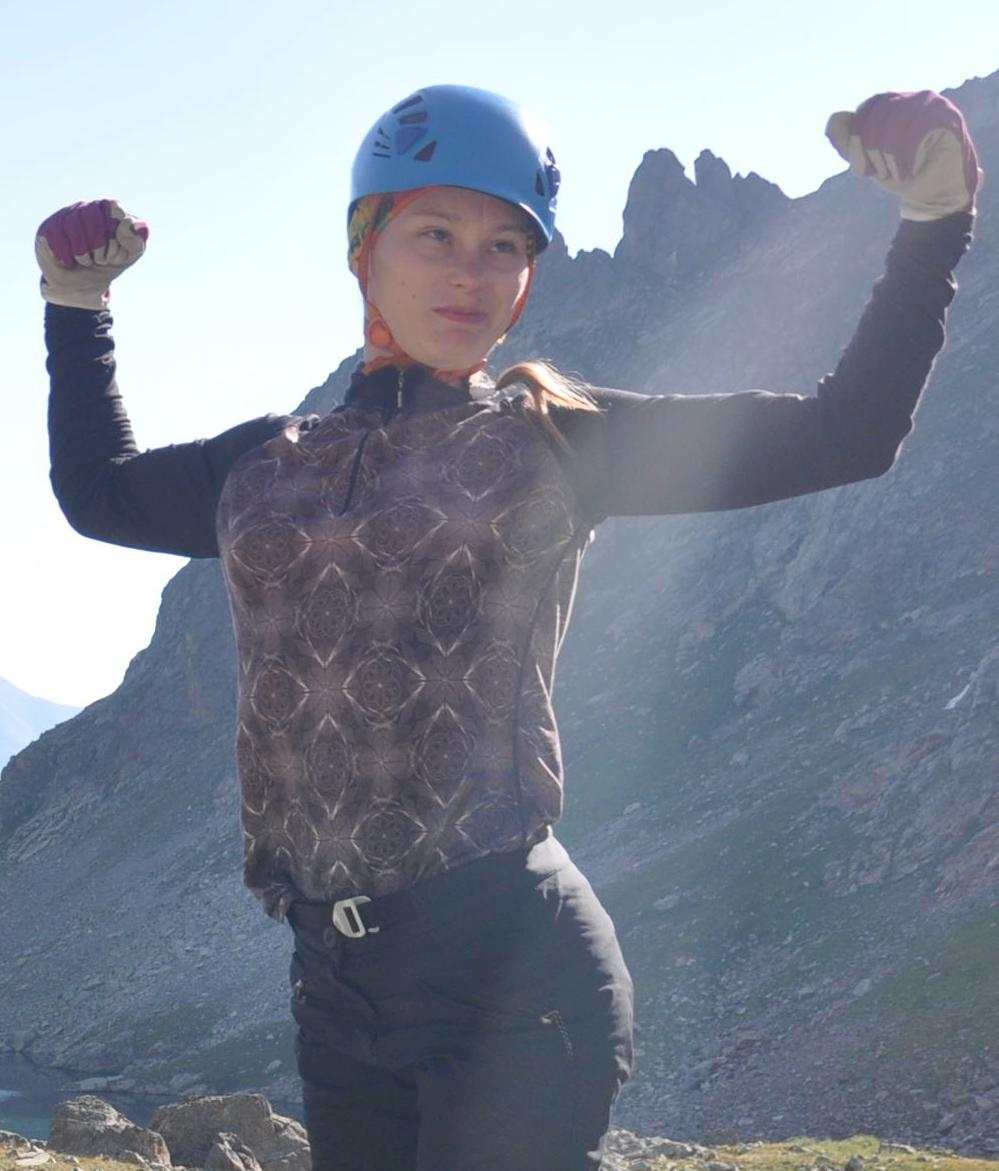
\includegraphics[width=\textwidth]{../pics/portraits/dasha_s}
	\end{minipage} &
	\begin{minipage}{\rozhasize}
		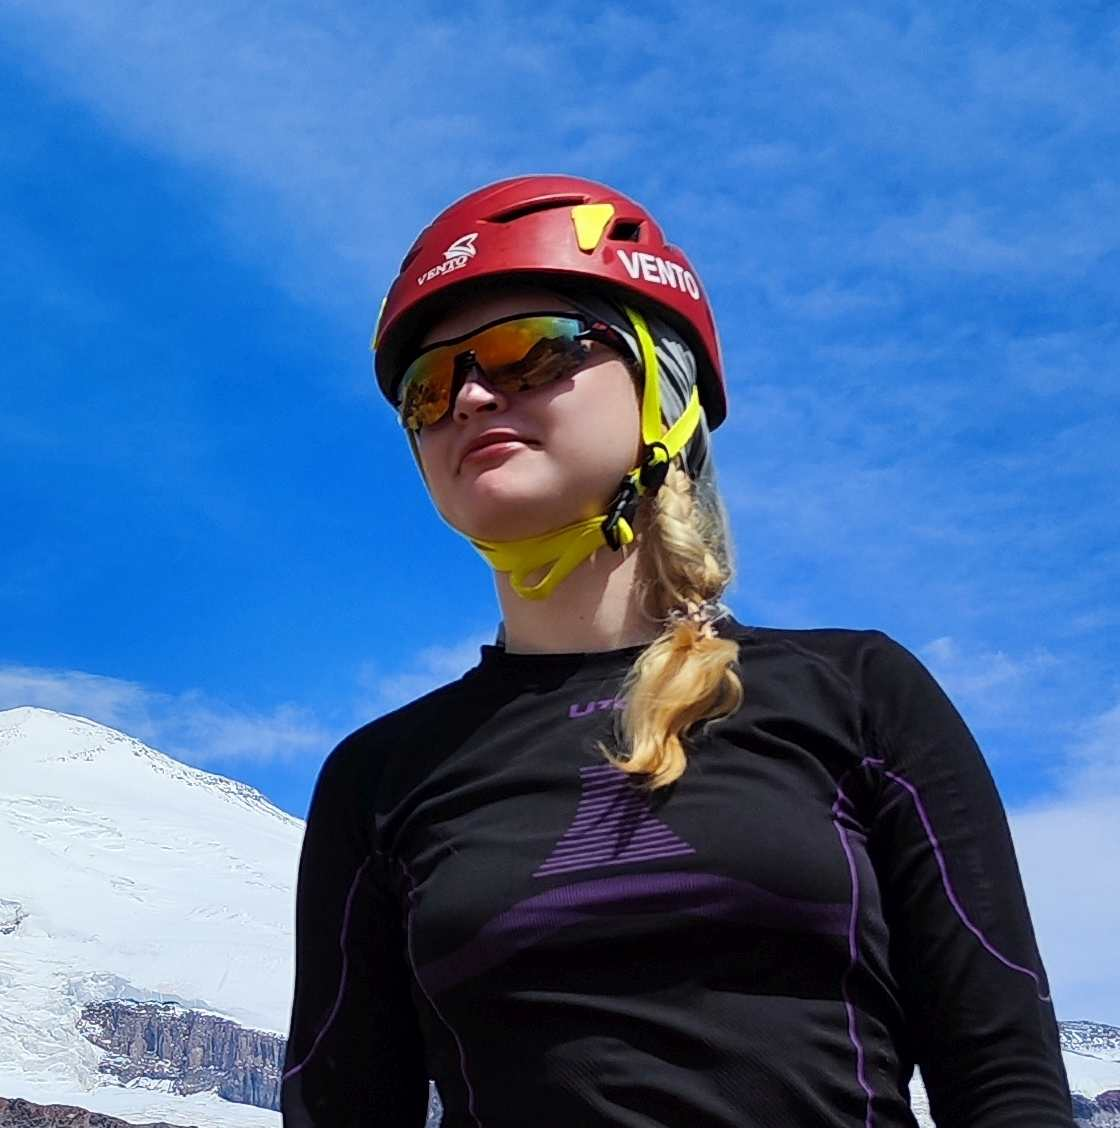
\includegraphics[width=\textwidth]{../pics/portraits/dasha_k}
	\end{minipage} &
	\begin{minipage}{\rozhasize}
		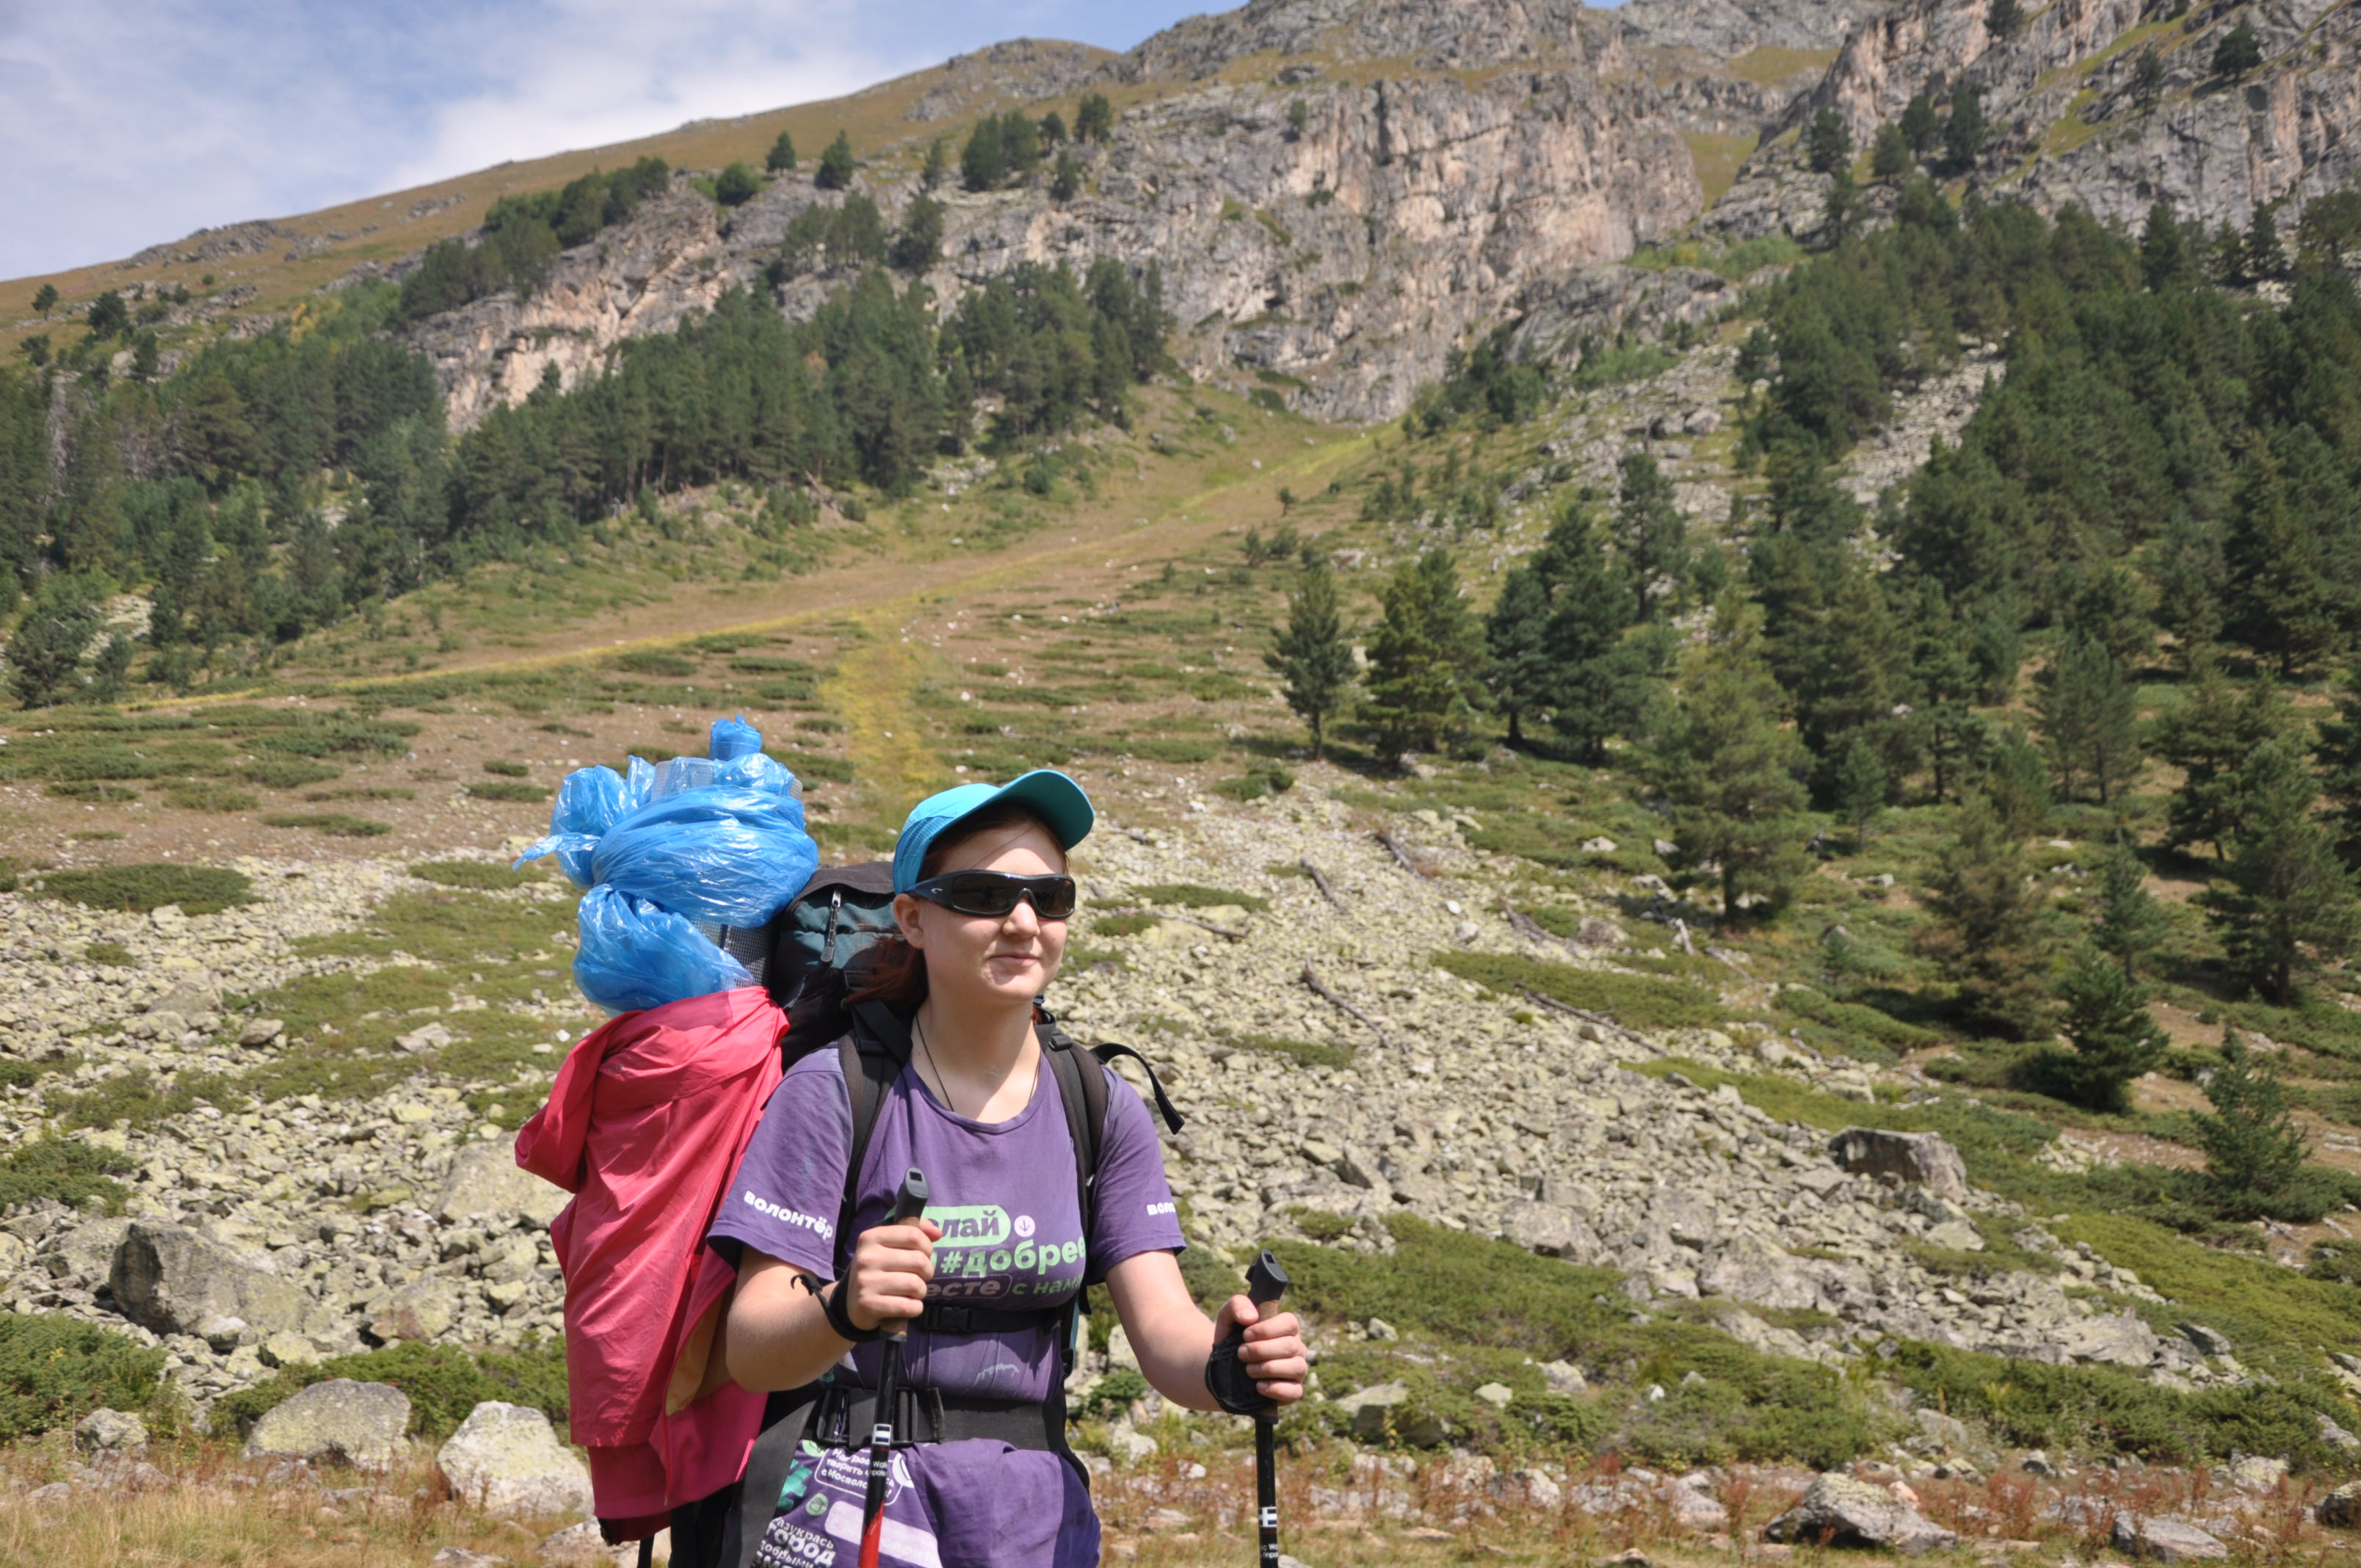
\includegraphics[width=\textwidth]{../pics/portraits/masha2}
	\end{minipage} &
	\begin{minipage}{\rozhasize}
		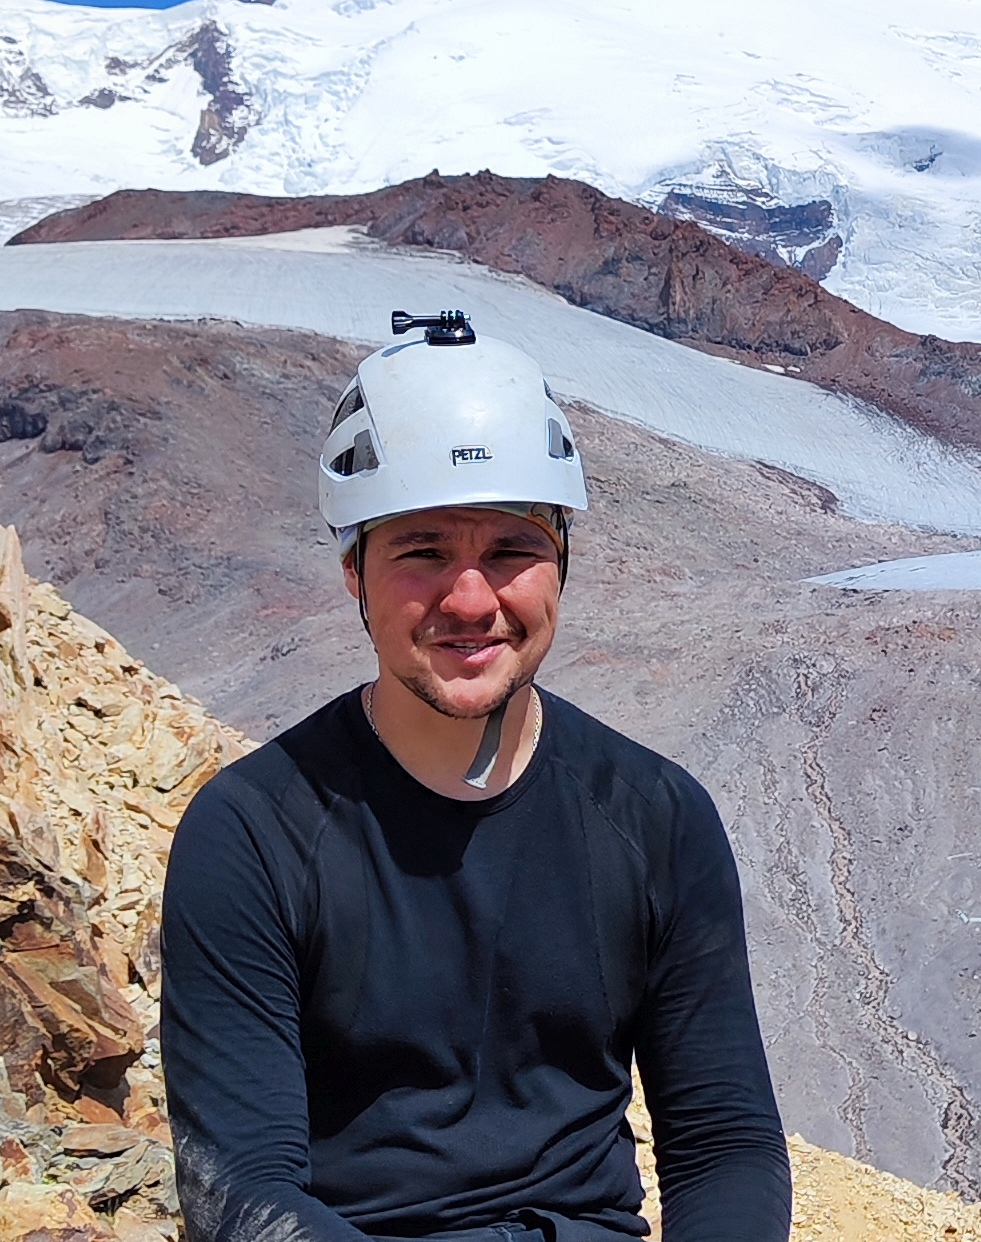
\includegraphics[width=\textwidth]{../pics/portraits/lesha_o1}
	\end{minipage} & 
	\begin{minipage}{\namesize}
		{\tiny
		Даша Снеговская\\
		Даша Казаринова\\
		Маша Семено\\
		Лёша Остапив}
		\end{minipage} \\
	
	\hline
	\begin{minipage}{\rozhasize}
	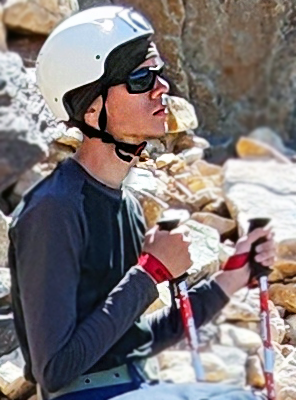
\includegraphics[width=\textwidth]{../pics/portraits/dima_d}
	\end{minipage} &
	\begin{minipage}{\rozhasize}
		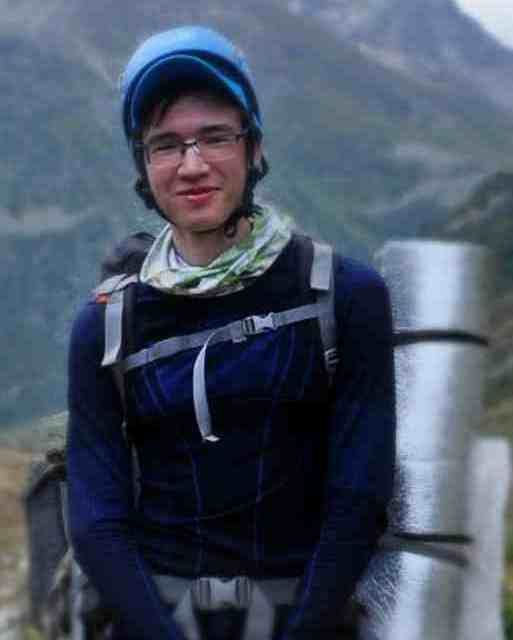
\includegraphics[width=\textwidth]{../pics/portraits/dima_s2}
	\end{minipage} &
	\begin{minipage}{\rozhasize}
		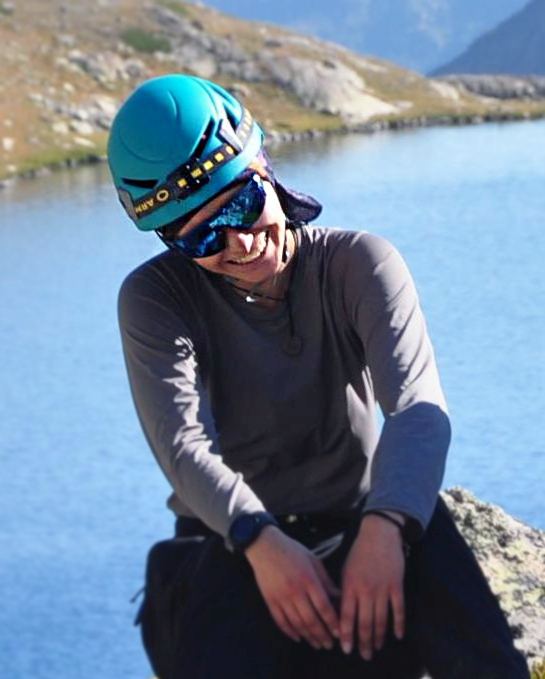
\includegraphics[width=\textwidth]{../pics/portraits/katya}
	\end{minipage} &
	\begin{minipage}{\rozhasize}
		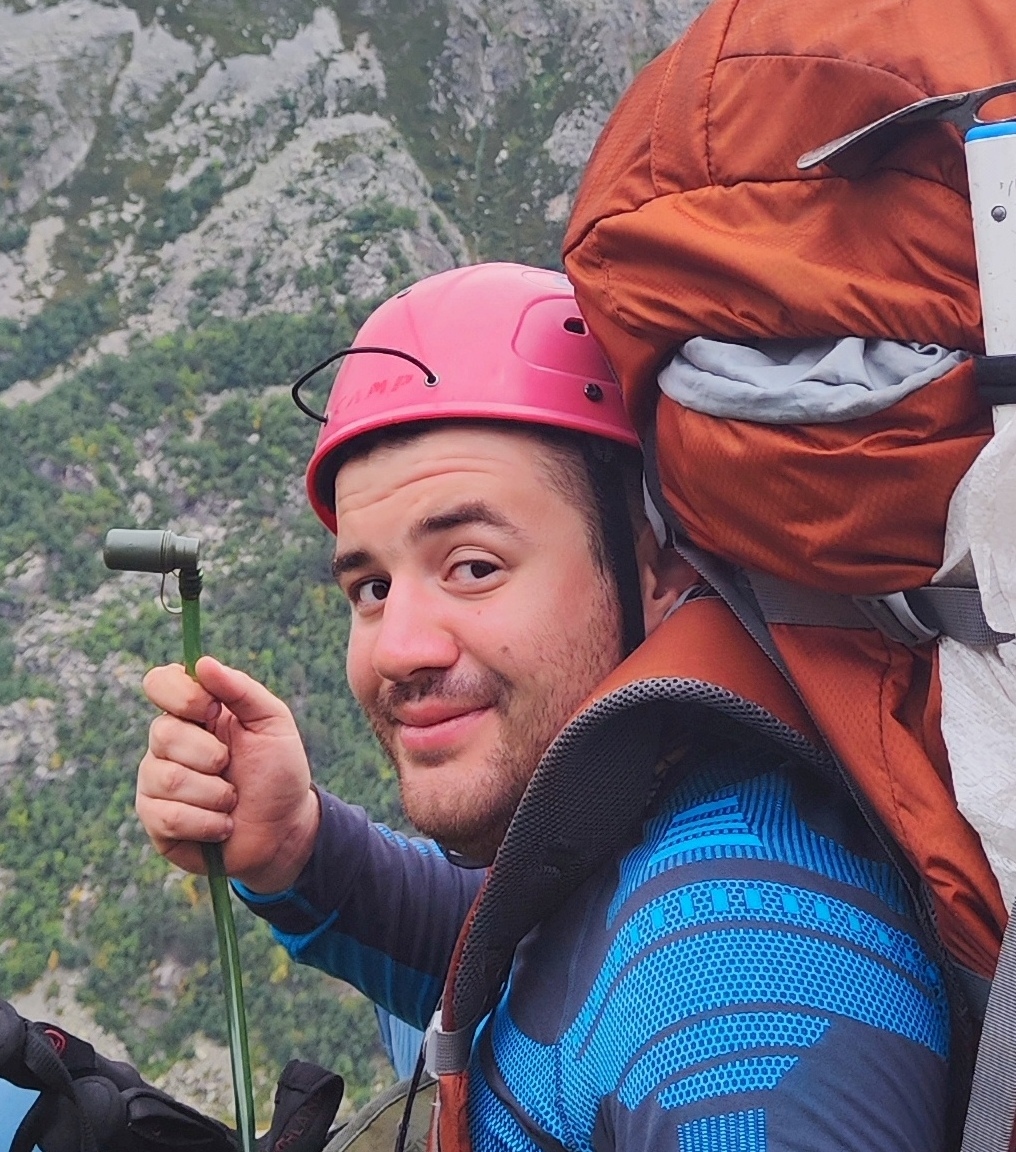
\includegraphics[width=\textwidth]{../pics/portraits/ilya_sh}
	\end{minipage} & 
	\begin{minipage}{\namesize}
		{\tiny
			Дима Дёмушкин\\
			Дима Сингалевич\\
			Катя Тюрина\\
			Илья Шалфеев}
	\end{minipage} \\
	
	\hline
	\begin{minipage}{\rozhasize}
	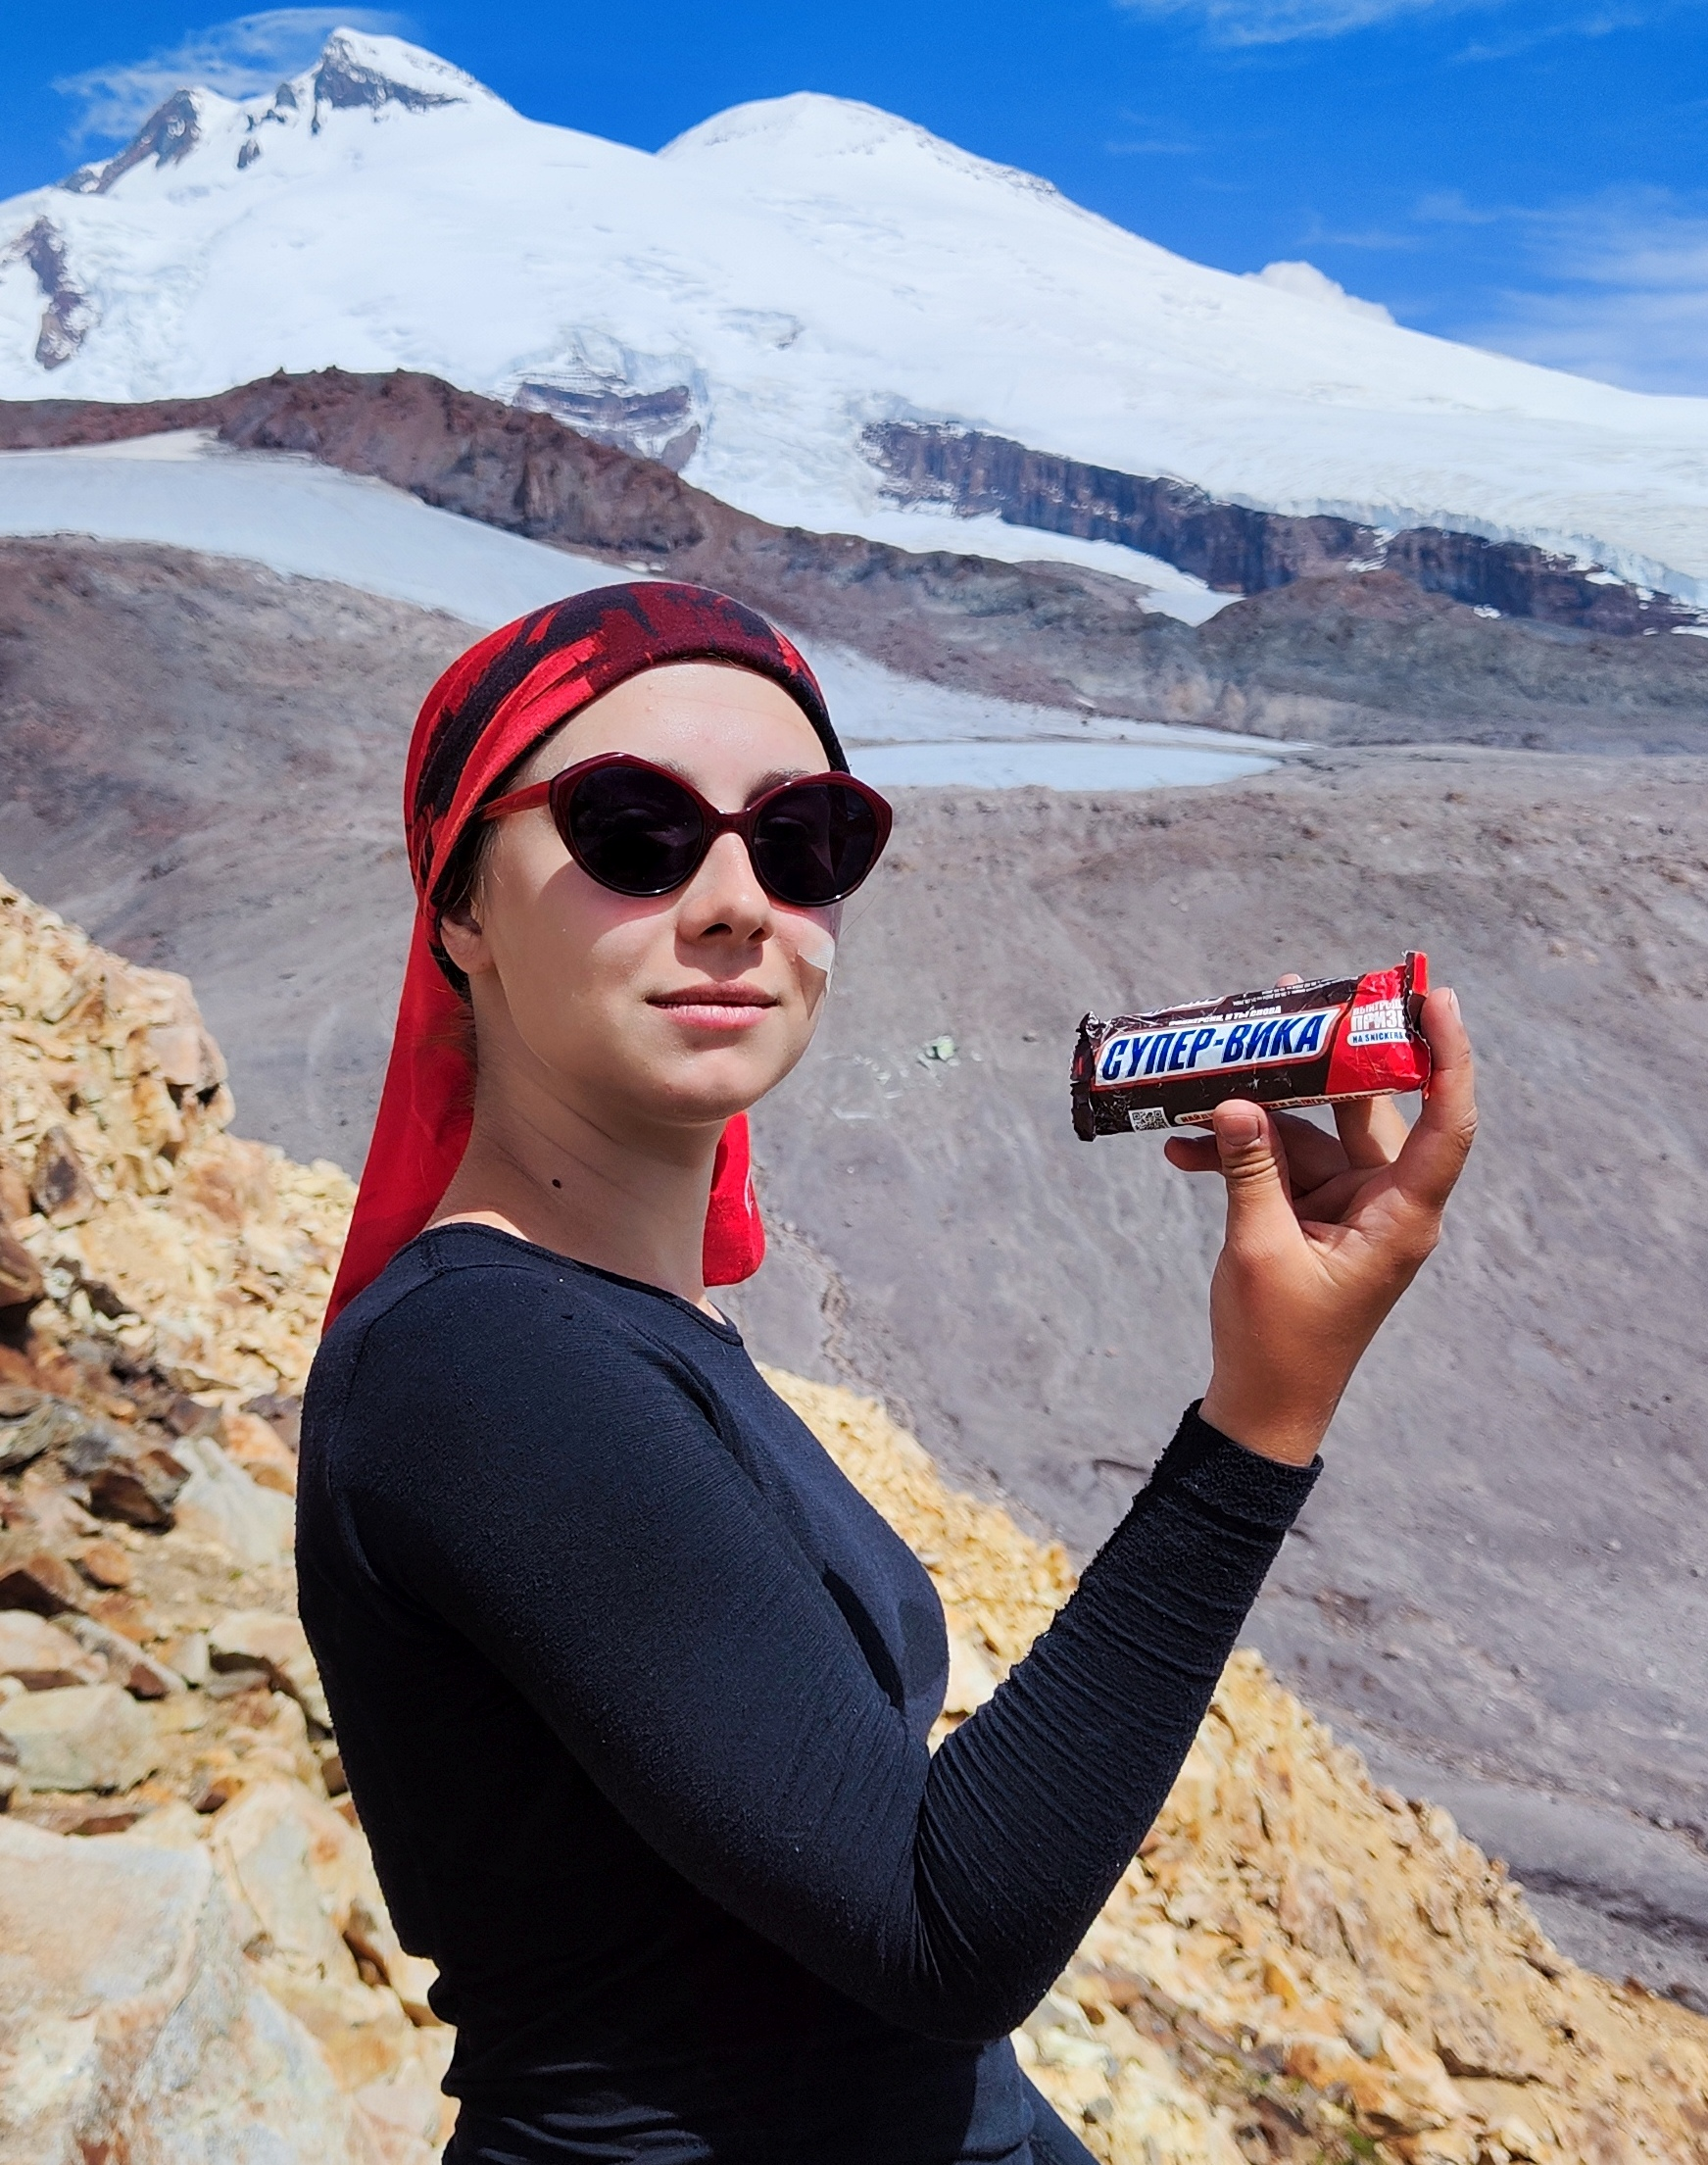
\includegraphics[width=\textwidth]{../pics/portraits/vika}
	\end{minipage} &
	\begin{minipage}{\rozhasize}
		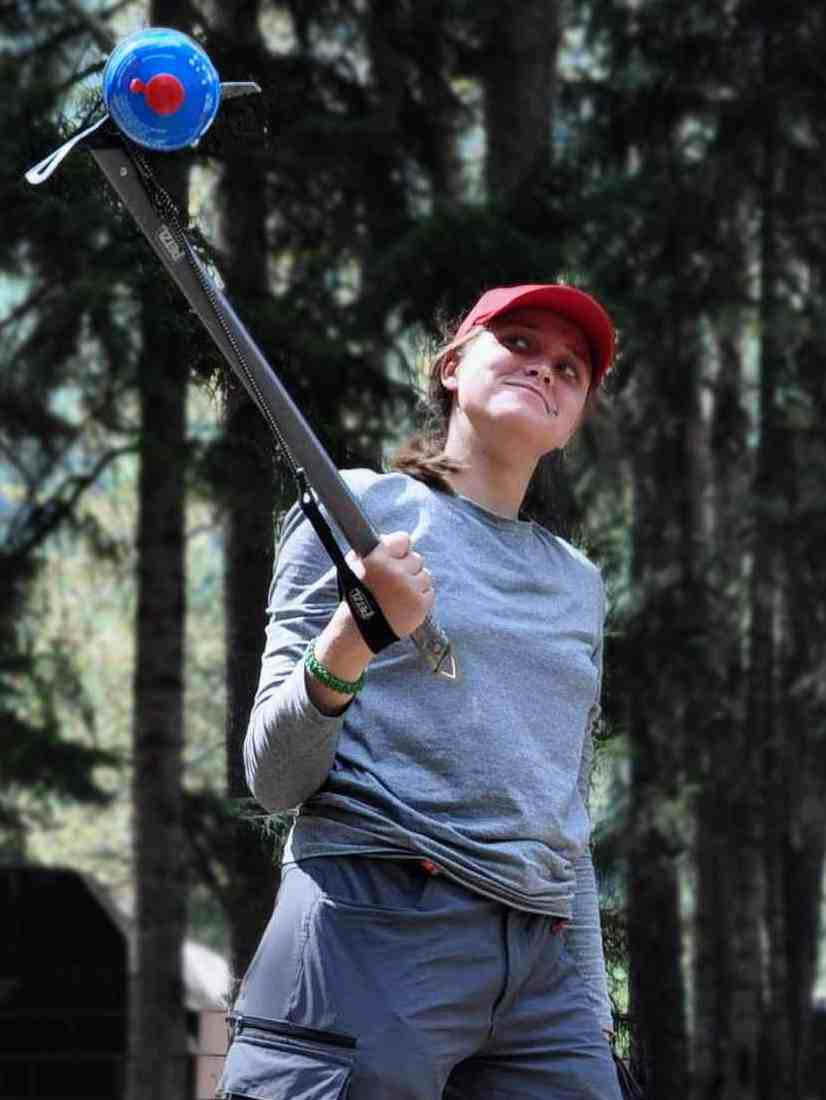
\includegraphics[width=\textwidth]{../pics/portraits/natasha1}
	\end{minipage} &
	\begin{minipage}{\rozhasize}
		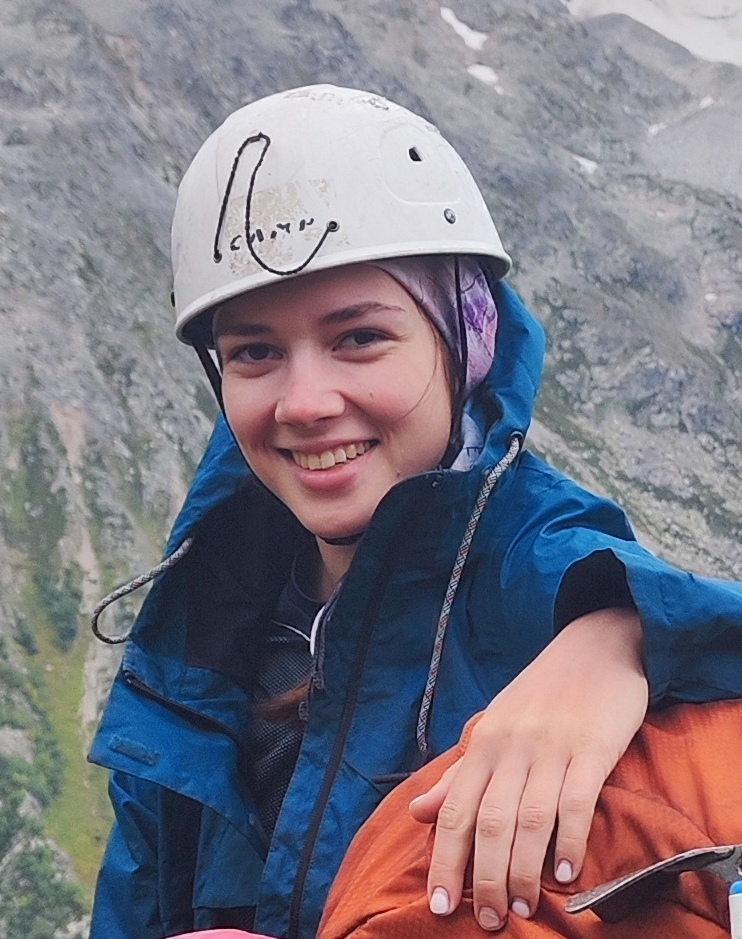
\includegraphics[width=\textwidth]{../pics/portraits/dasha_m}
	\end{minipage} &
	\begin{minipage}{\rozhasize}
		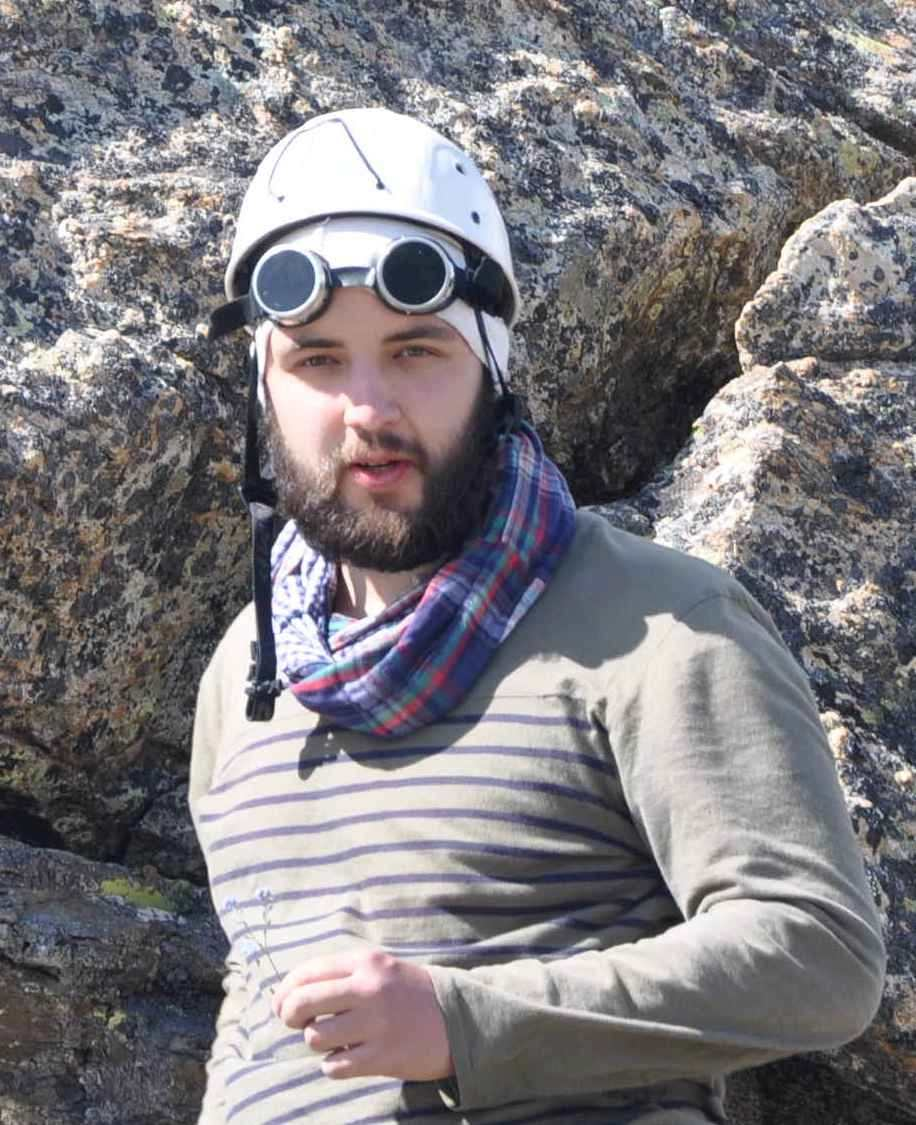
\includegraphics[width=\textwidth]{../pics/portraits/gosha}
	\end{minipage} & 
	\begin{minipage}{\namesize}
		{\tiny
			Вика Суровцева\\
			Наташа Миронова\\
			Даша Мерзликина\\
			Гоша Корнилов}
	\end{minipage} \\	
\end{tabular}	
\end{frame}
	
	\subsection{Идея похода}
	\begin{frame}
	\frametitle{Почему Гвандра?}
	\begin{itemize}
		\item Дёшево и быстро ехать
		\item Красиво и разнообразно
		\item Посмотреть Эльбрус
		\item Скатать у Андрея Королёва
	\end{itemize}
	\textbf{Идея похода}~--- пройти чисто, при условии, что группа новичковая
	\end{frame}
	
	\subsection{Список препятствий}
	\begin{frame}
		\setbeamercovered{transparent}
		\frametitle{Список препятствий}
		\begin{enumerate}
			\item<+-> Уллу-Кёль Восточный, 3050 (1А)
			\item<+-> Джалпаккол Северный, 3411  (1А)
			\item<+-> Кичкинекол Малый, 3206 (1А)
			\item<+-> Перемётный, 3255 (1А)
			\item<+-> Хотютау, 3546 (1А)
		\end{enumerate}
	\centering
	\includegraphics<1>[height=0.5\textheight]{../pics/passes/ullu_kuel}%
	\includegraphics<2>[height=0.5\textheight]{../pics/passes/dzhalpakkol}%
	\includegraphics<3>[height=0.5\textheight]{../pics/passes/kich}%
	\includegraphics<4>[height=0.5\textheight]{../pics/passes/perem}%
	\includegraphics<5>[height=0.5\textheight]{../pics/passes/hot}%

	\end{frame}
	
	\subsection{Трек}
	
	\begin{frame}
		\frametitle{Трек}
		\rotatebox{90}{
			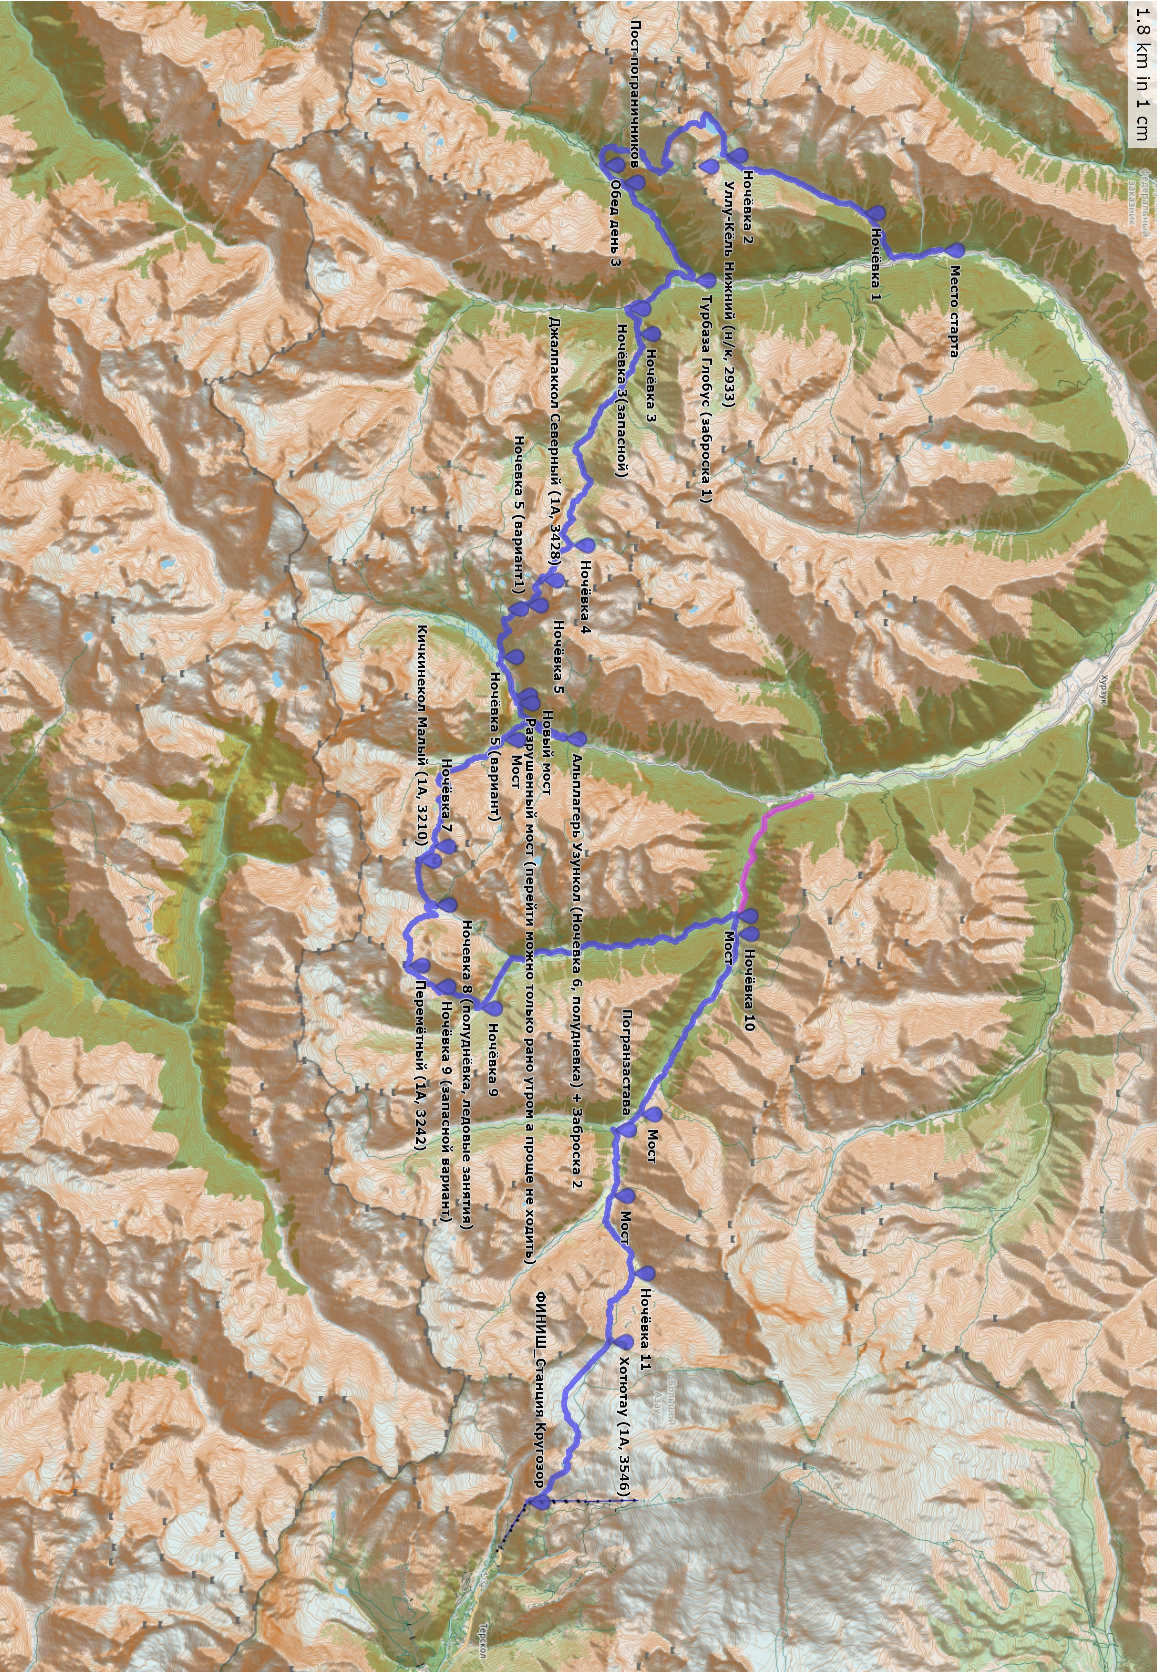
\includegraphics[width=0.68\linewidth]{../pics/route}}		
	\end{frame}
	
	%------------------------------------------------
	\section{Отчёт по дням}
	
		\begin{frame}
	\frametitle{День 1. 18 августа}
	\framesubtitle{Старт~--- д.р. Кичкинакол Уллукёльский} % Optional subtitle
	\begin{columns}[c] % The "c" option specifies centered vertical alignment while the "t" option is used for top vertical alignment
		\begin{column}{0.45\textwidth} % Left column width
			\begin{itemize}
				\item Перепаковка, формирование заброски
				\item Прошли \textbf{5.3} км
				\item ЧХВ: 2:46
				\item Набор/сброс: \textcolor{darkred}{\textbf{+650}}/\textcolor{darkblue}{\textbf{-0}}~м
			\end{itemize}
			
		\end{column}
		\begin{column}{0.5\textwidth} % Right column width
			\centering
			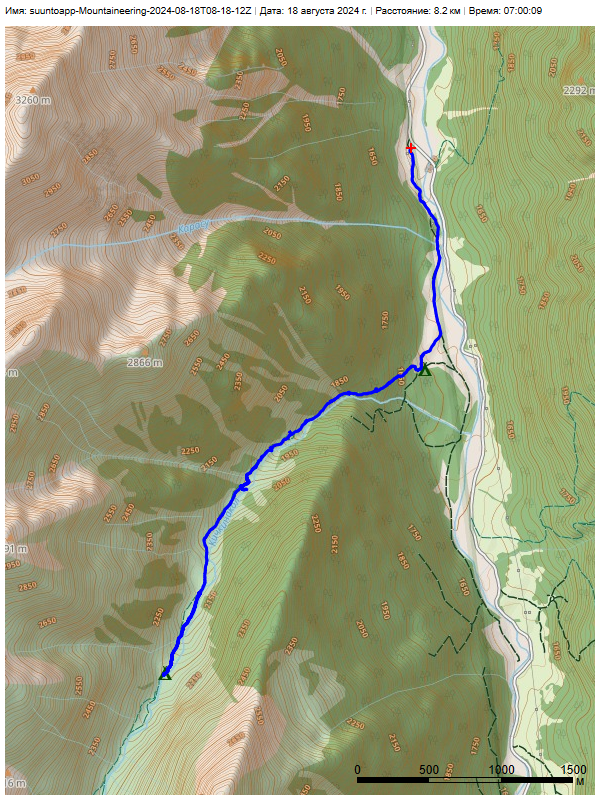
\includegraphics[width=\linewidth]{../pics/mini_maps/18}
		\end{column}
	\end{columns}
\end{frame}

\begin{frame}
	\frametitle{Выход на маршрут}
	\framesubtitle{День 1, 18 августа}
	\centering
	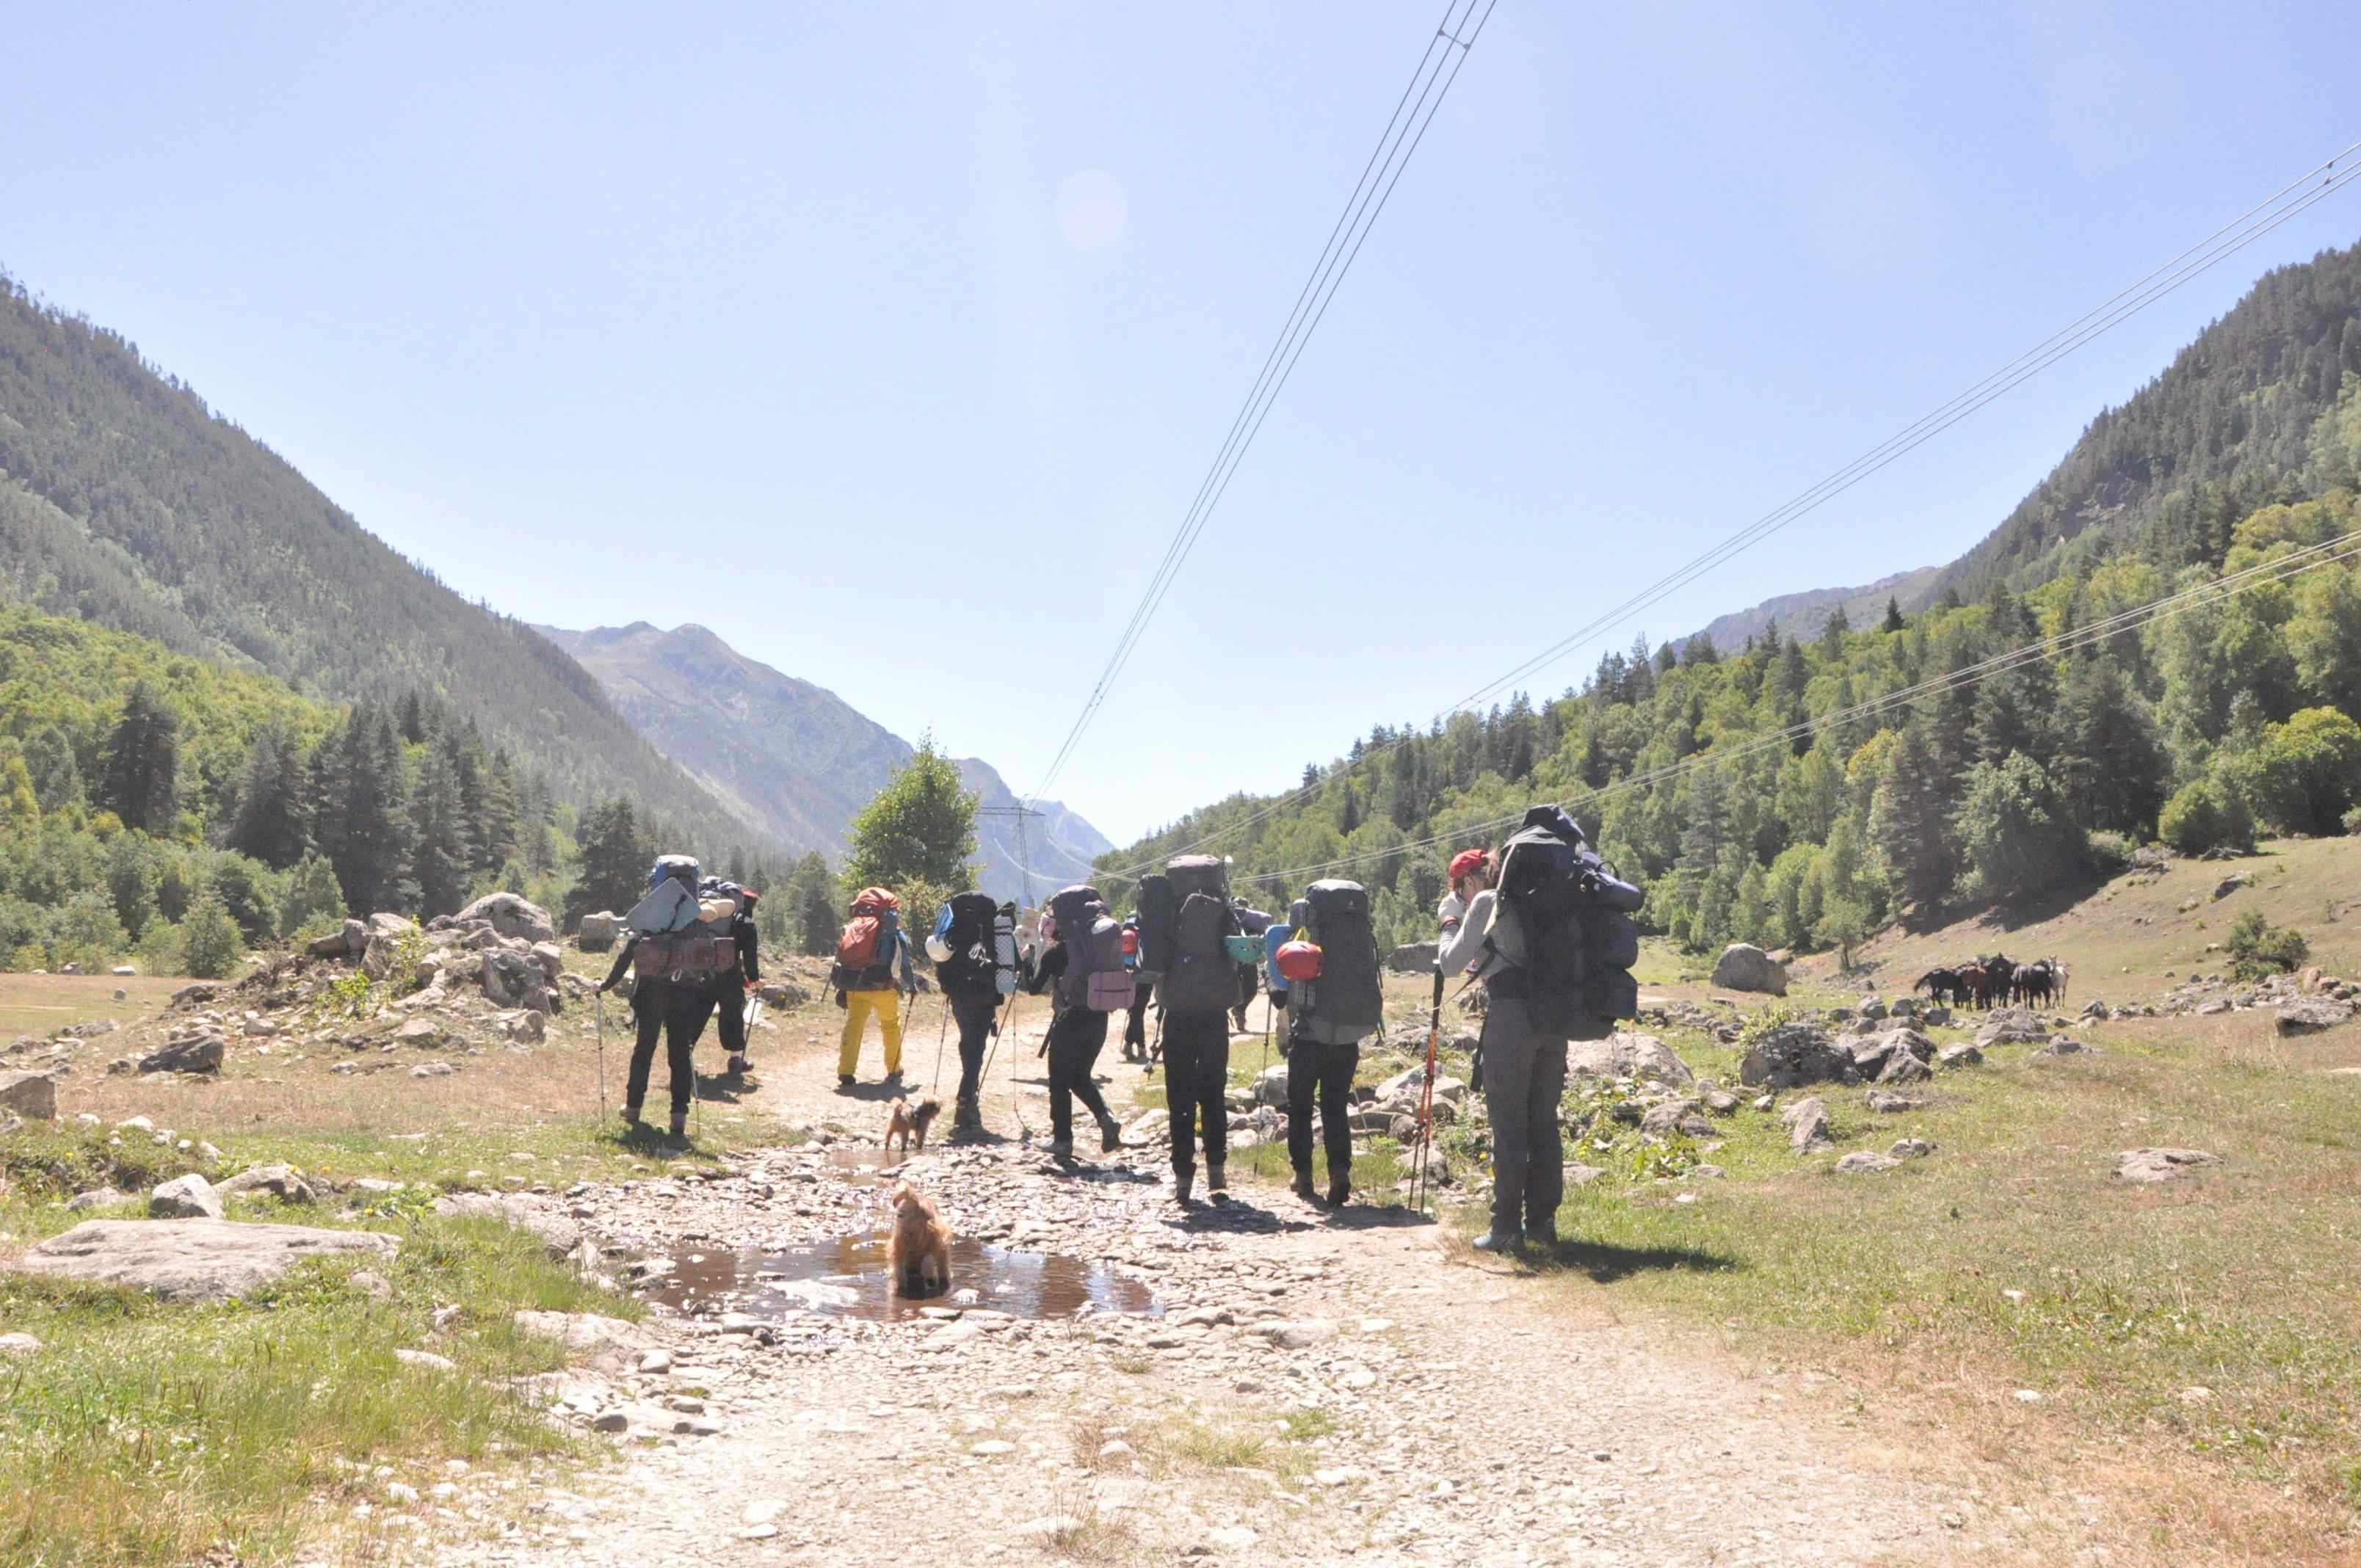
\includegraphics[width=\linewidth]{../pics/DSC_0412}
\end{frame}

\begin{frame}
	\frametitle{Даша М. с собачьками}
	\framesubtitle{День 1, 18 августа} 
	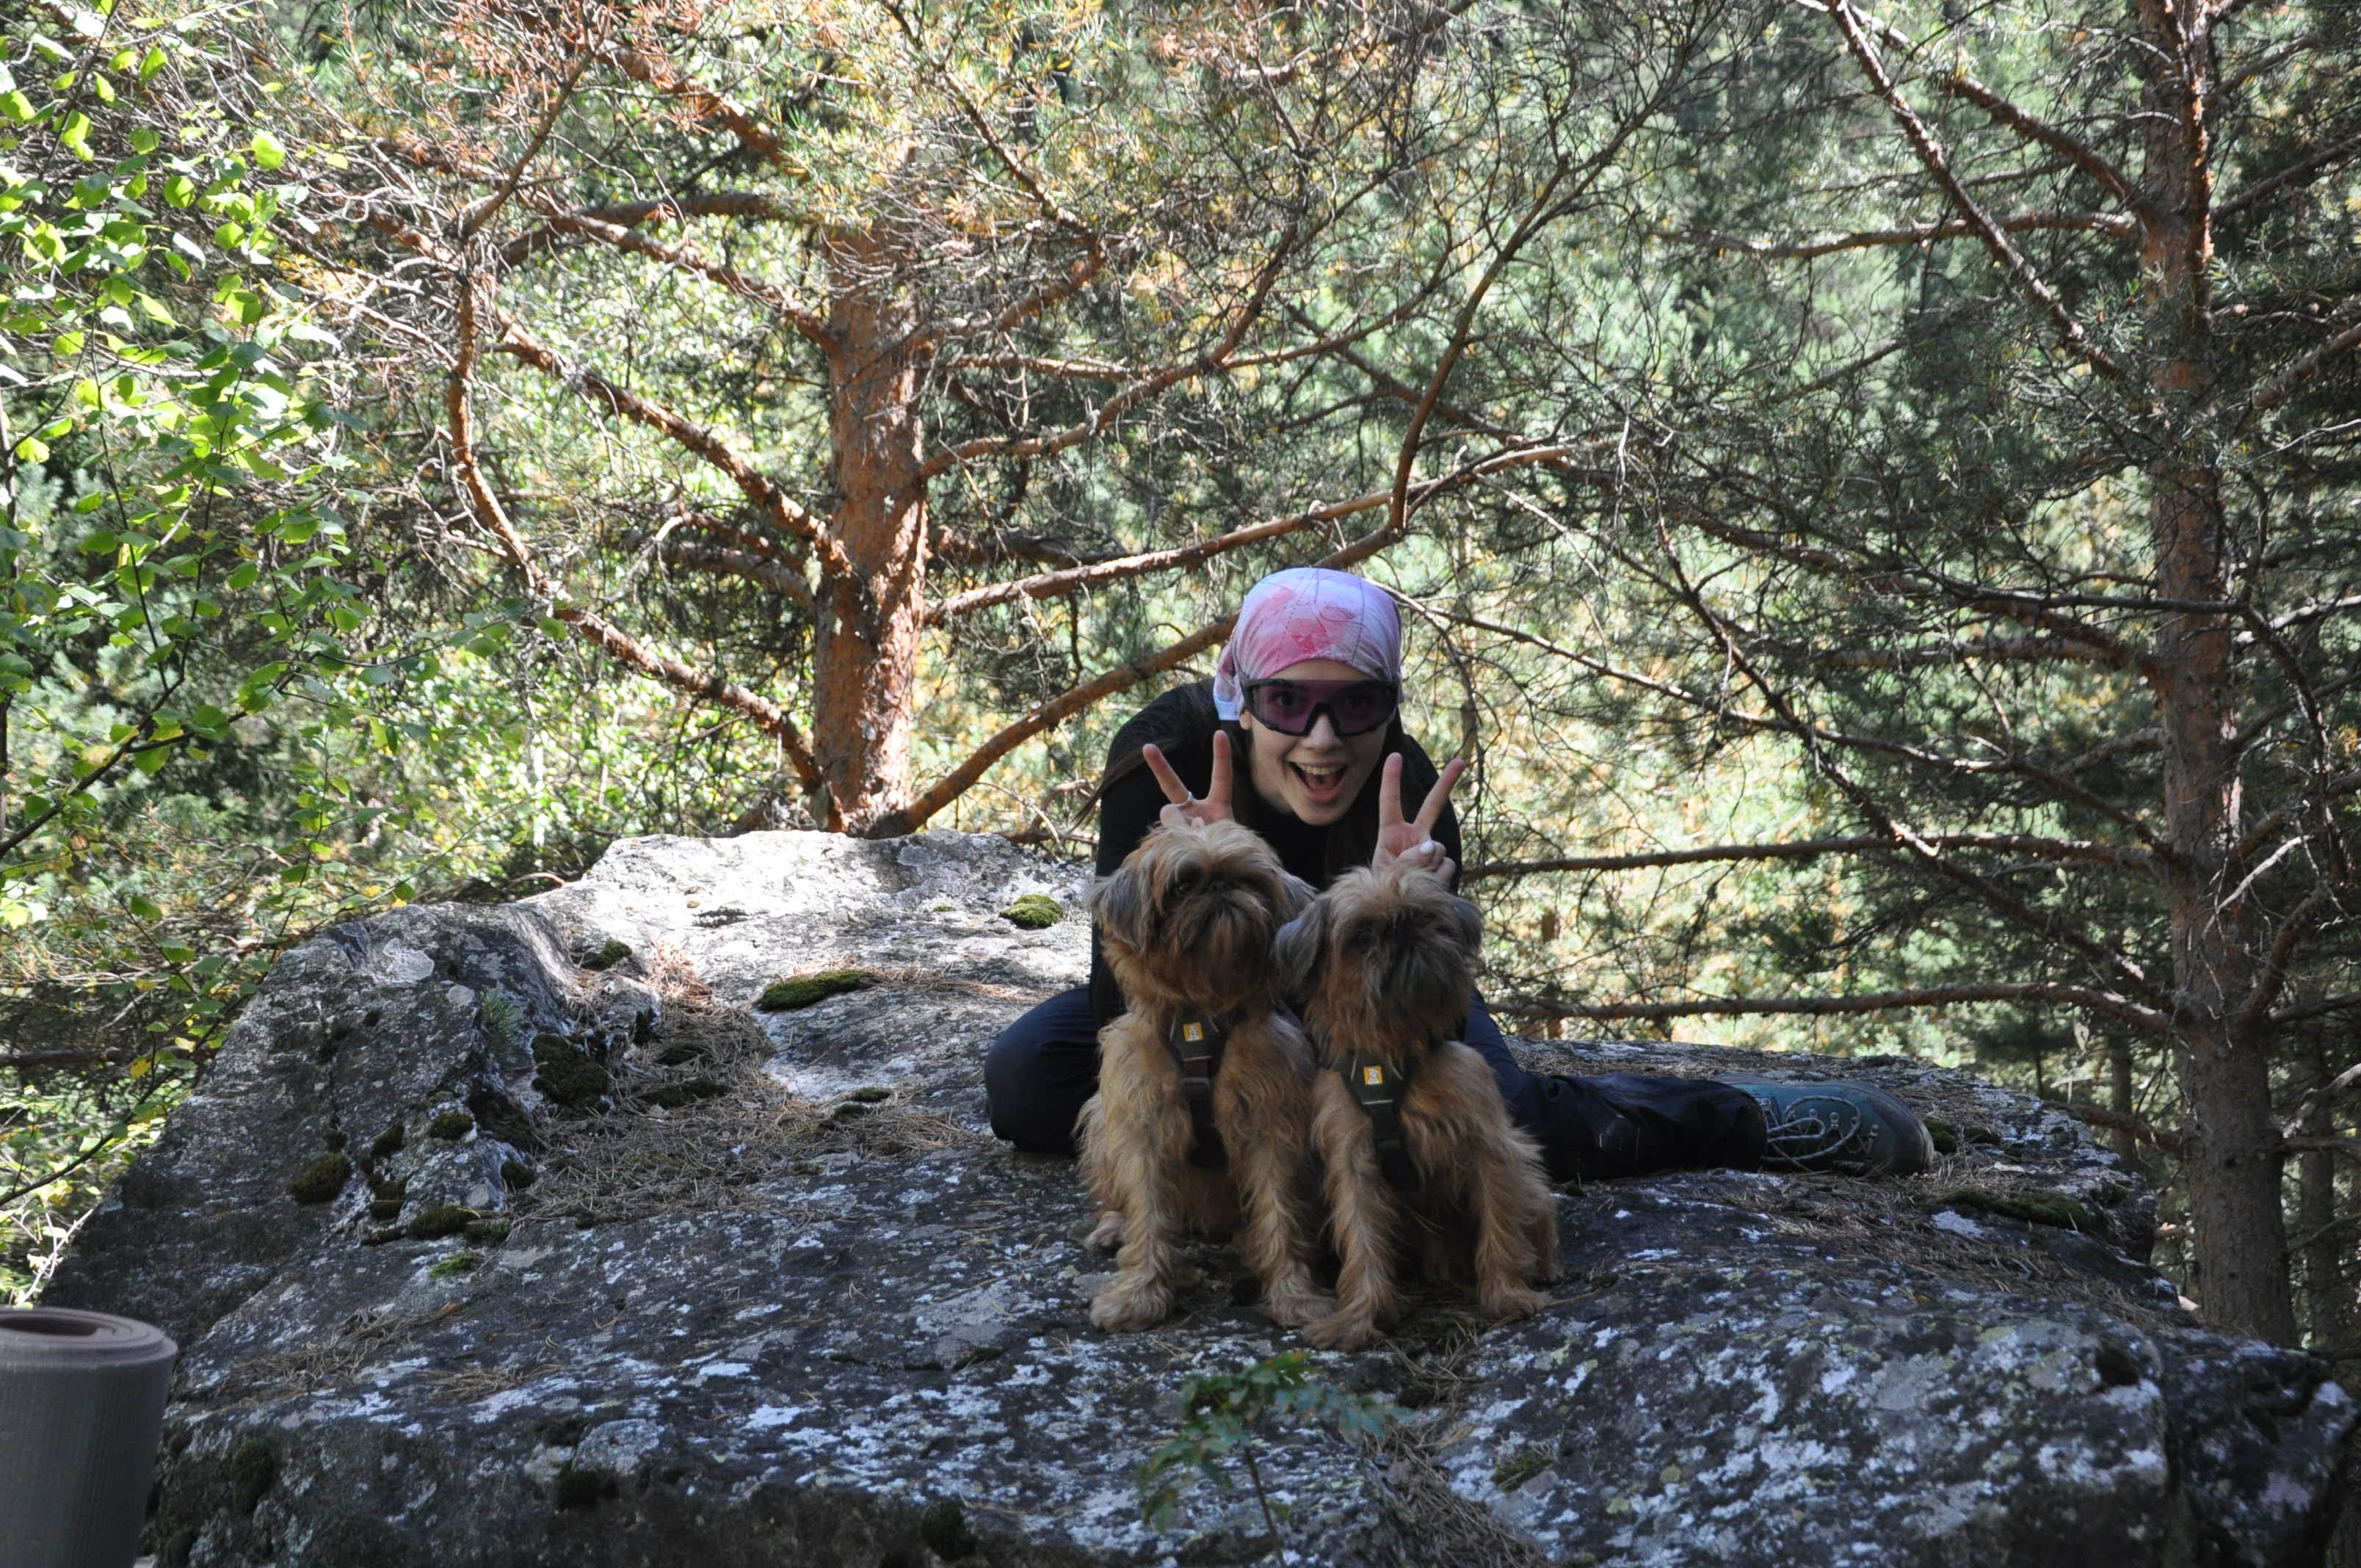
\includegraphics[width=\textwidth]{../pics/DSC_0475}
%	{\tiny
%		\begin{minipage}{\fourpicsize}
%			\centering
%			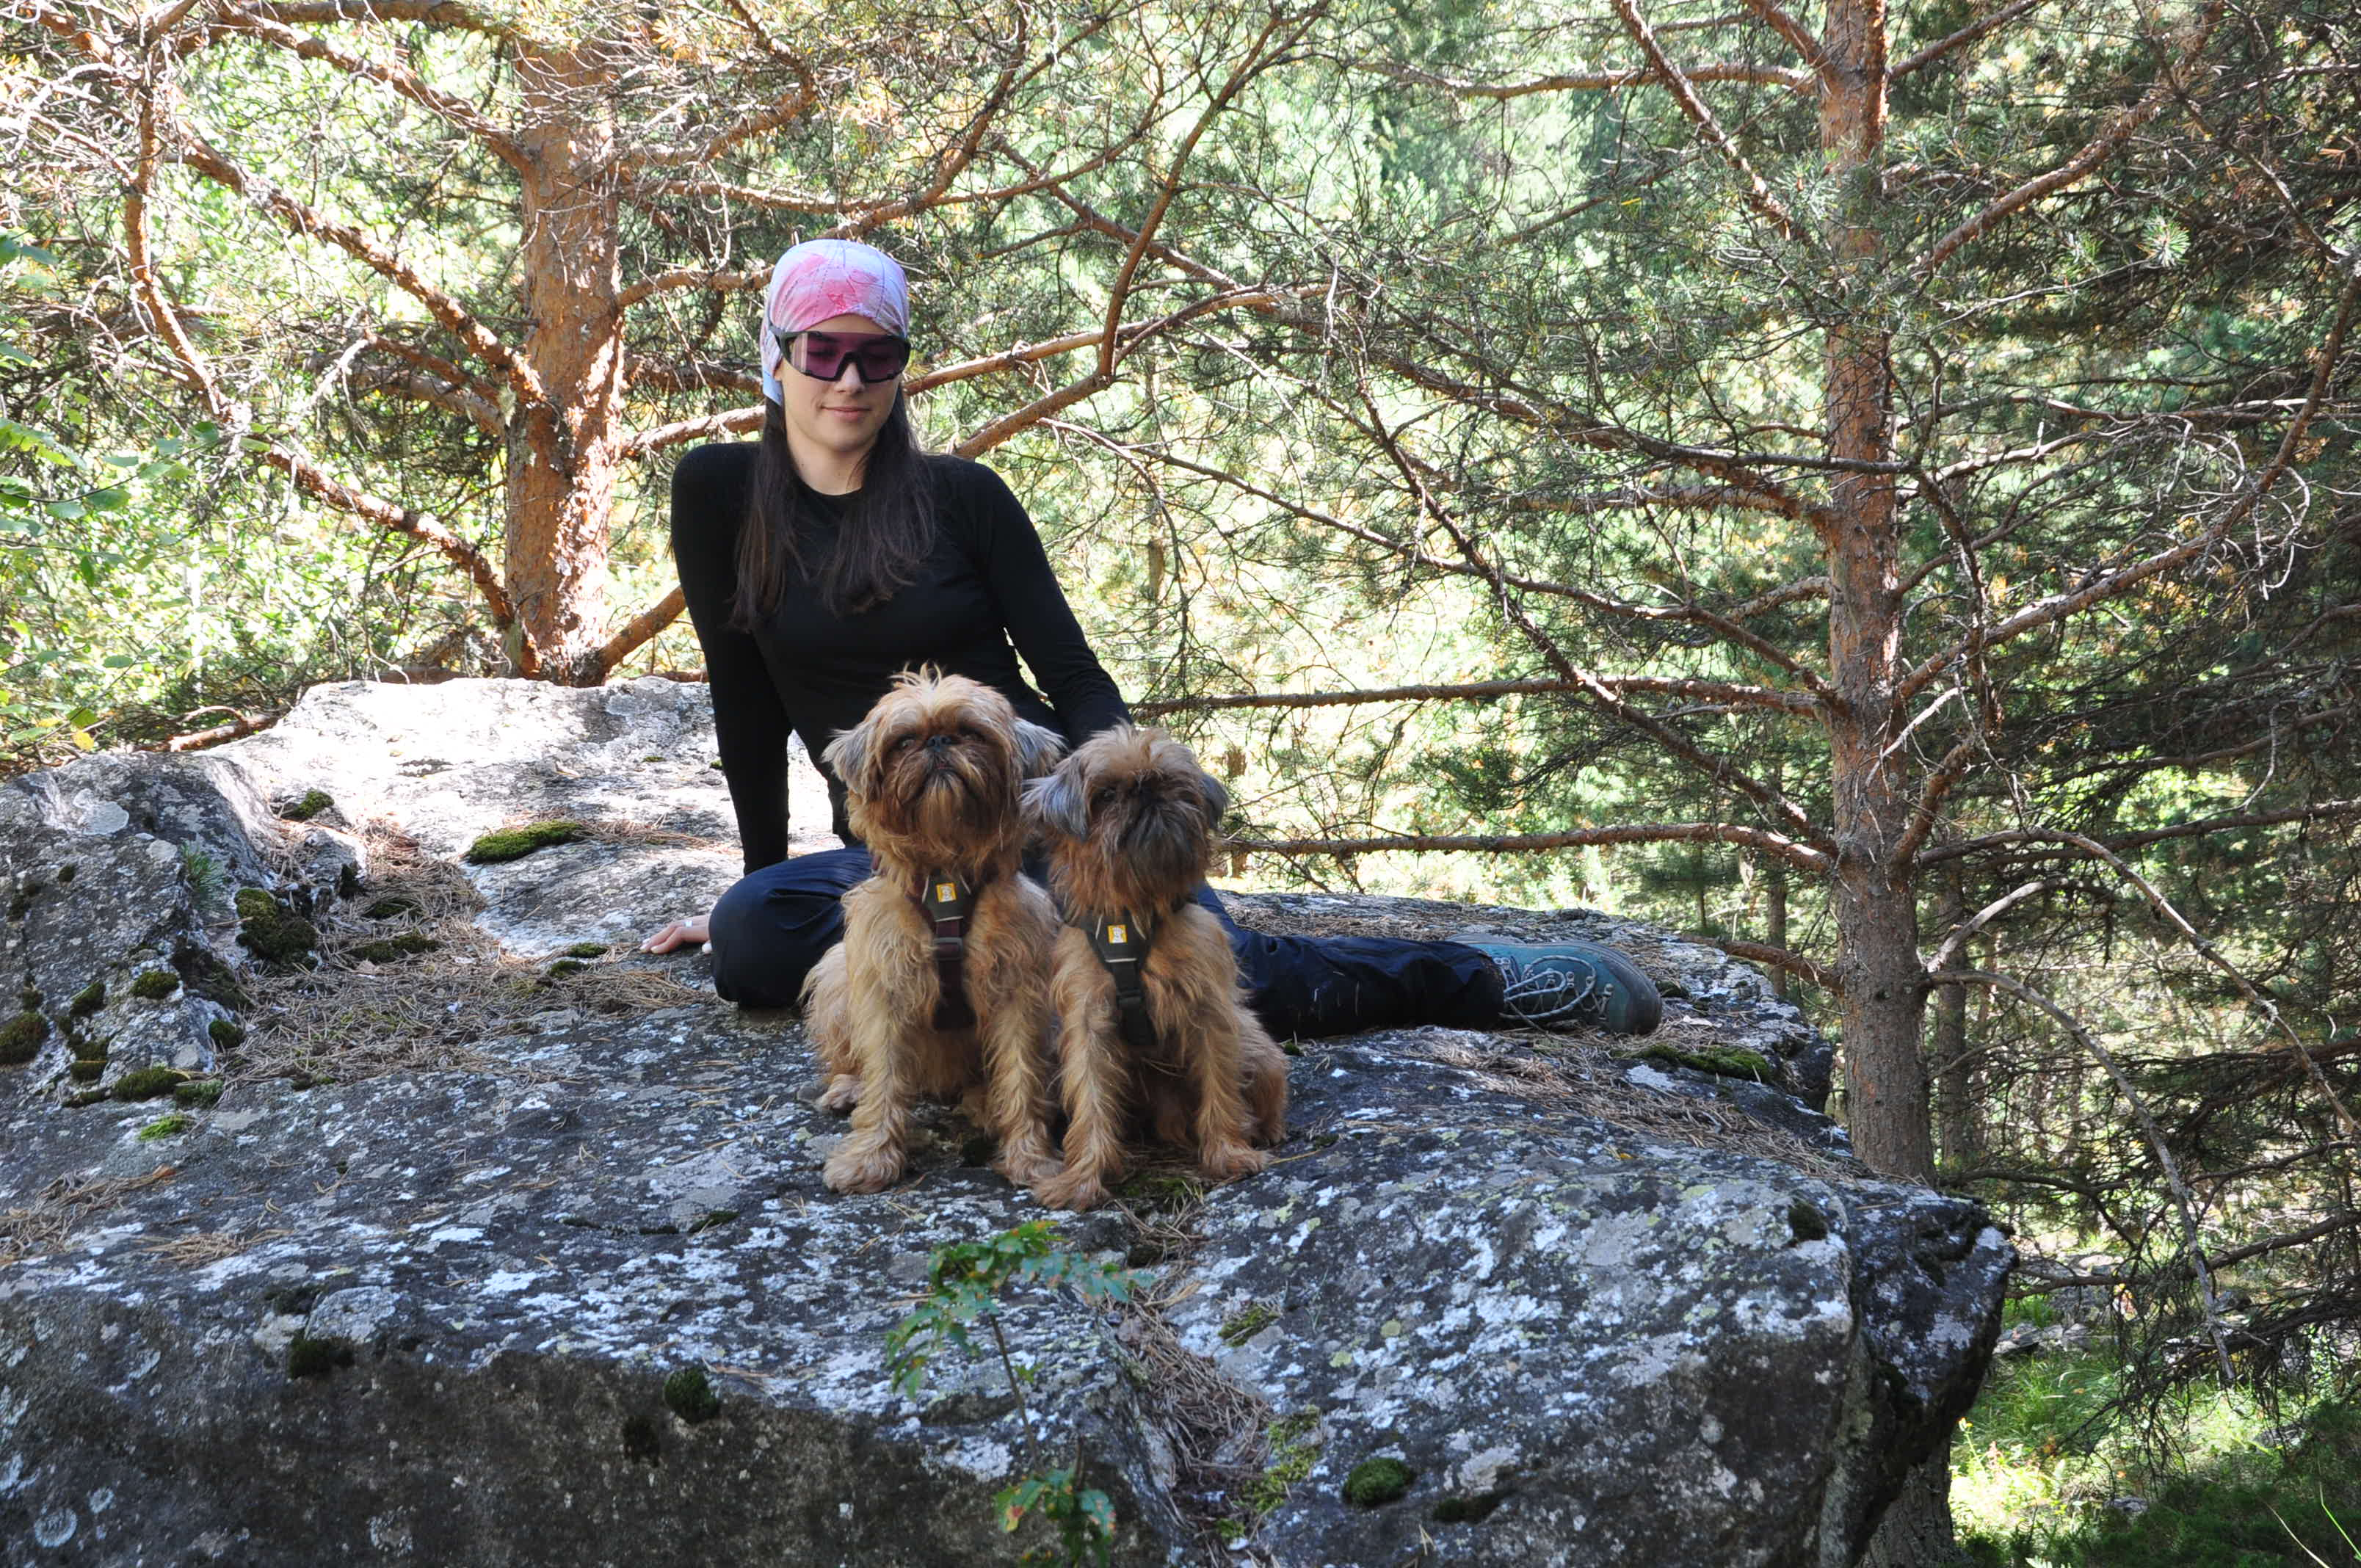
\includegraphics[width=\textwidth]{../pics/DSC_0472}			
%
%		\end{minipage}
%		\hfill
%		\begin{minipage}{\fourpicsize}
%			\centering
%			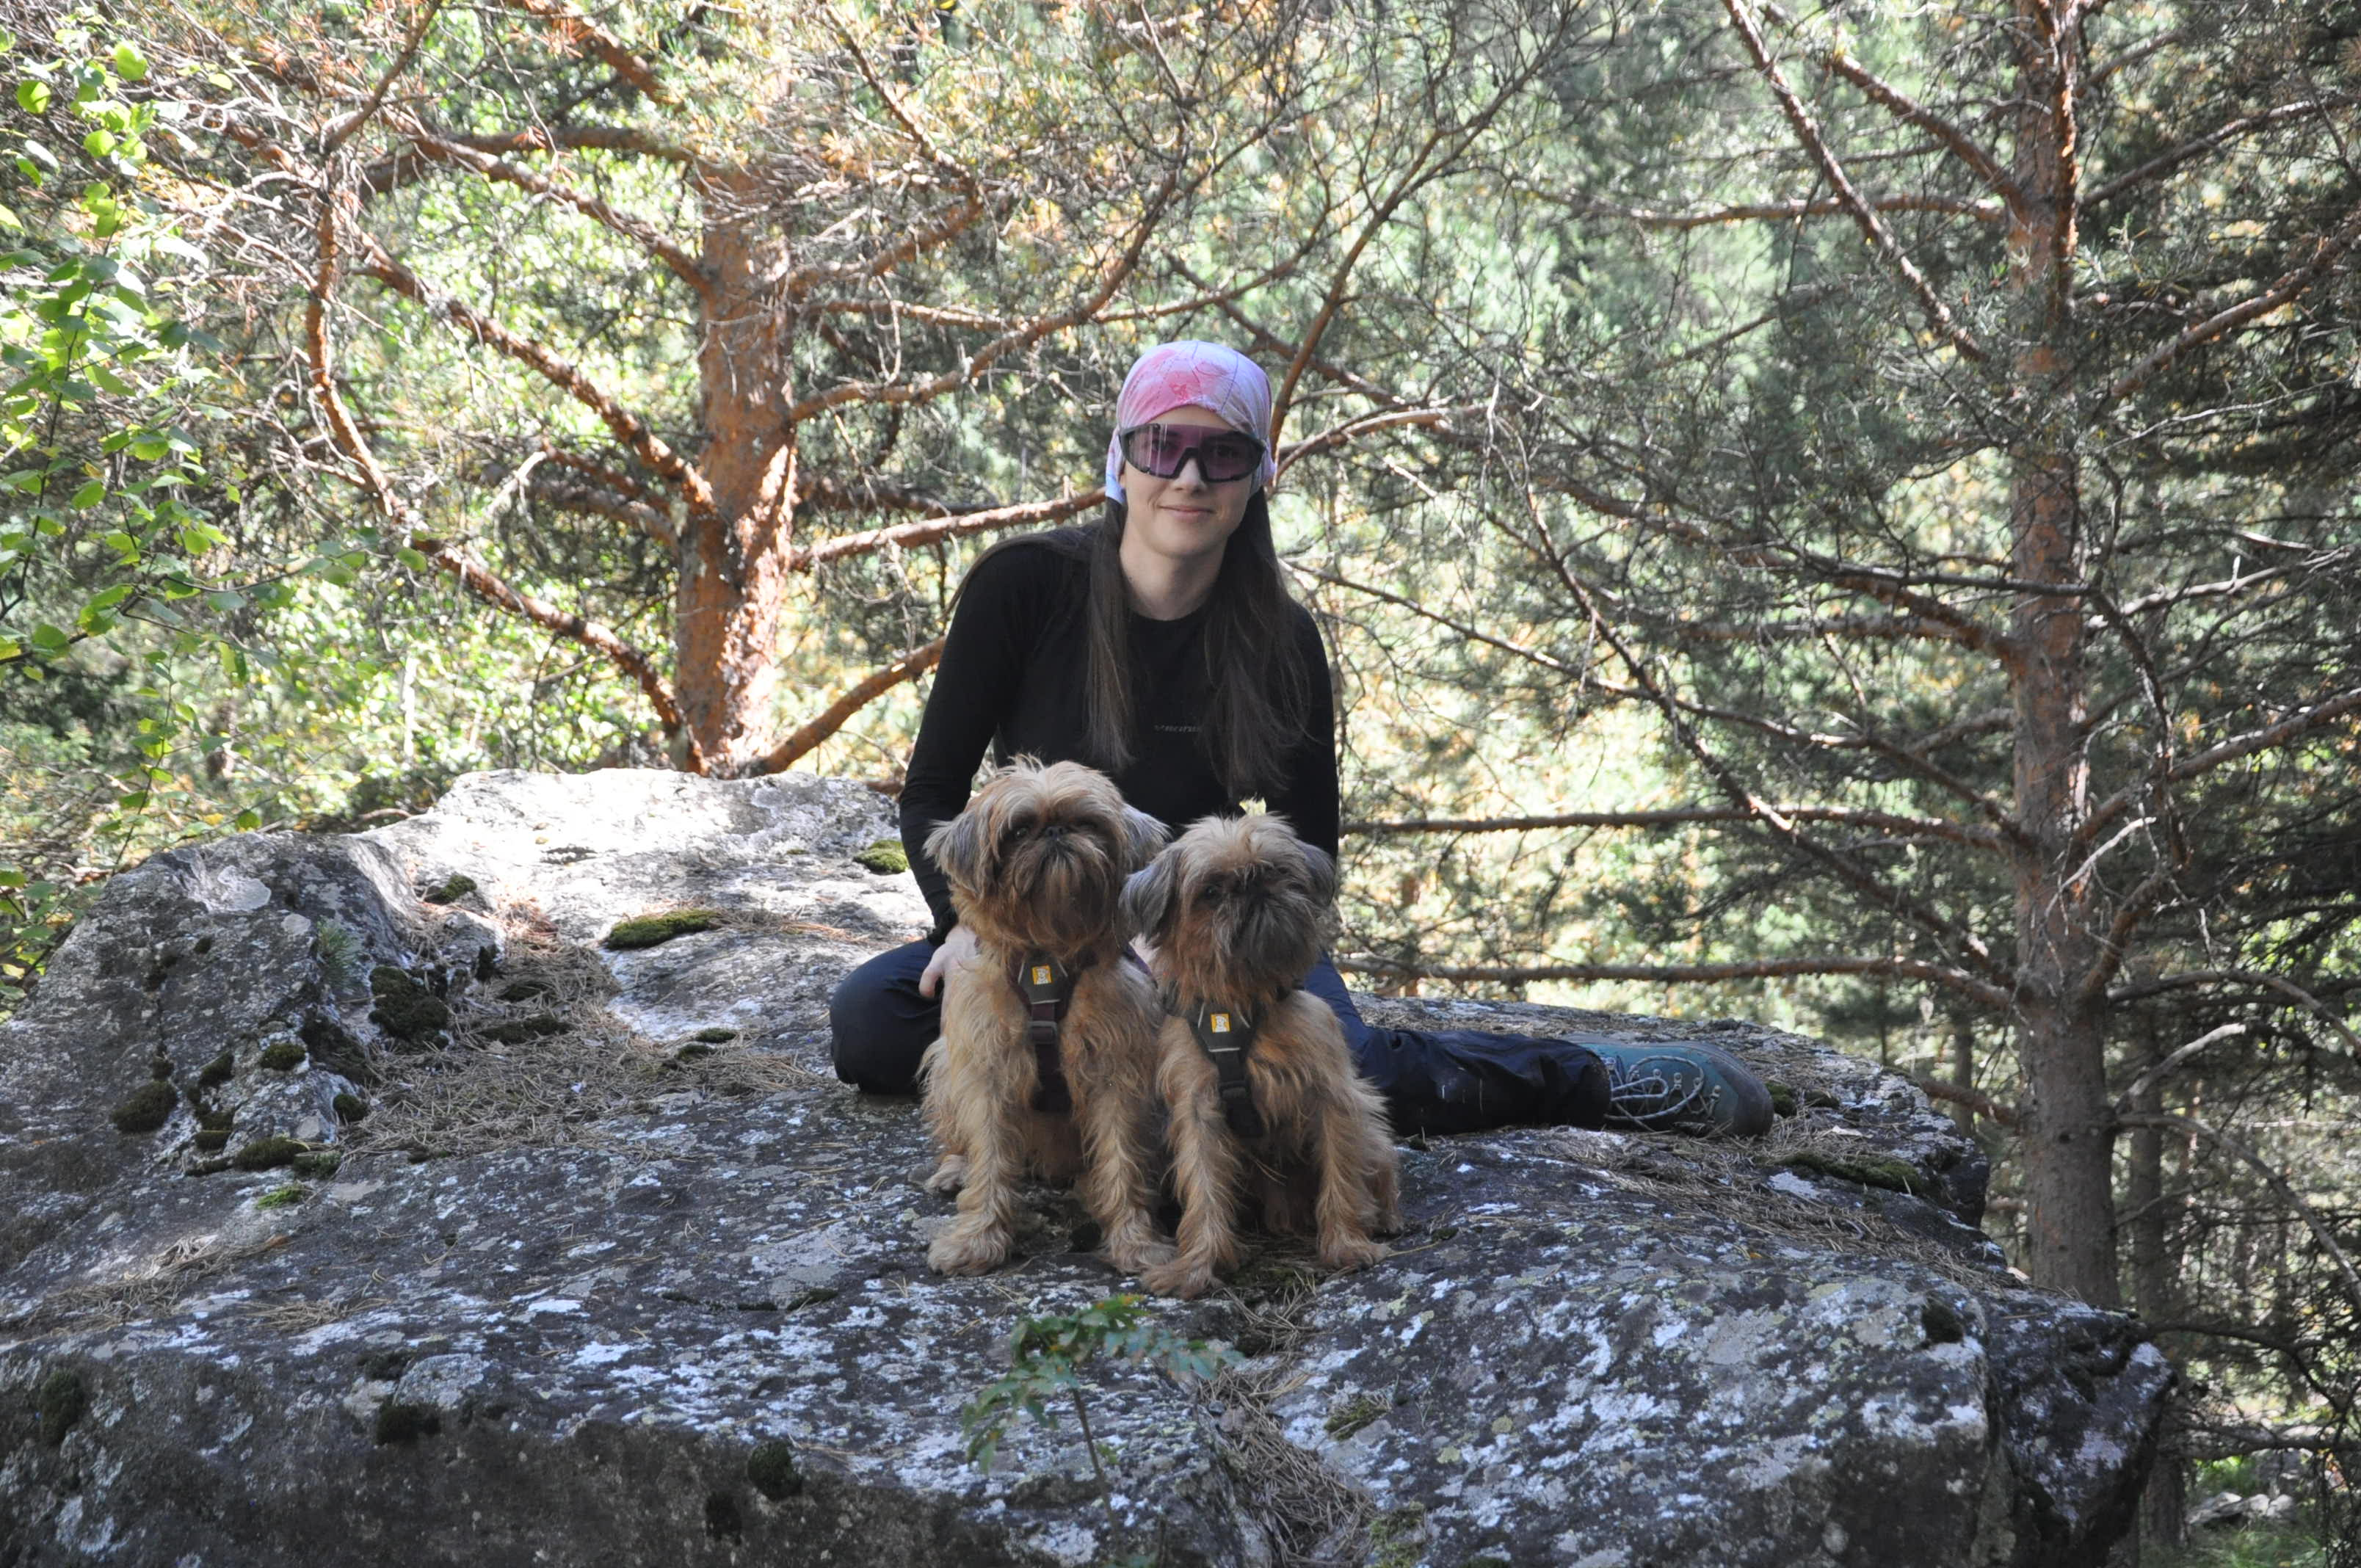
\includegraphics[width=\textwidth]{../pics/DSC_0474}			
%
%		\end{minipage}
%		\vfill
%		\centering
%		\begin{minipage}{\fourpicsize}
%			\centering
%			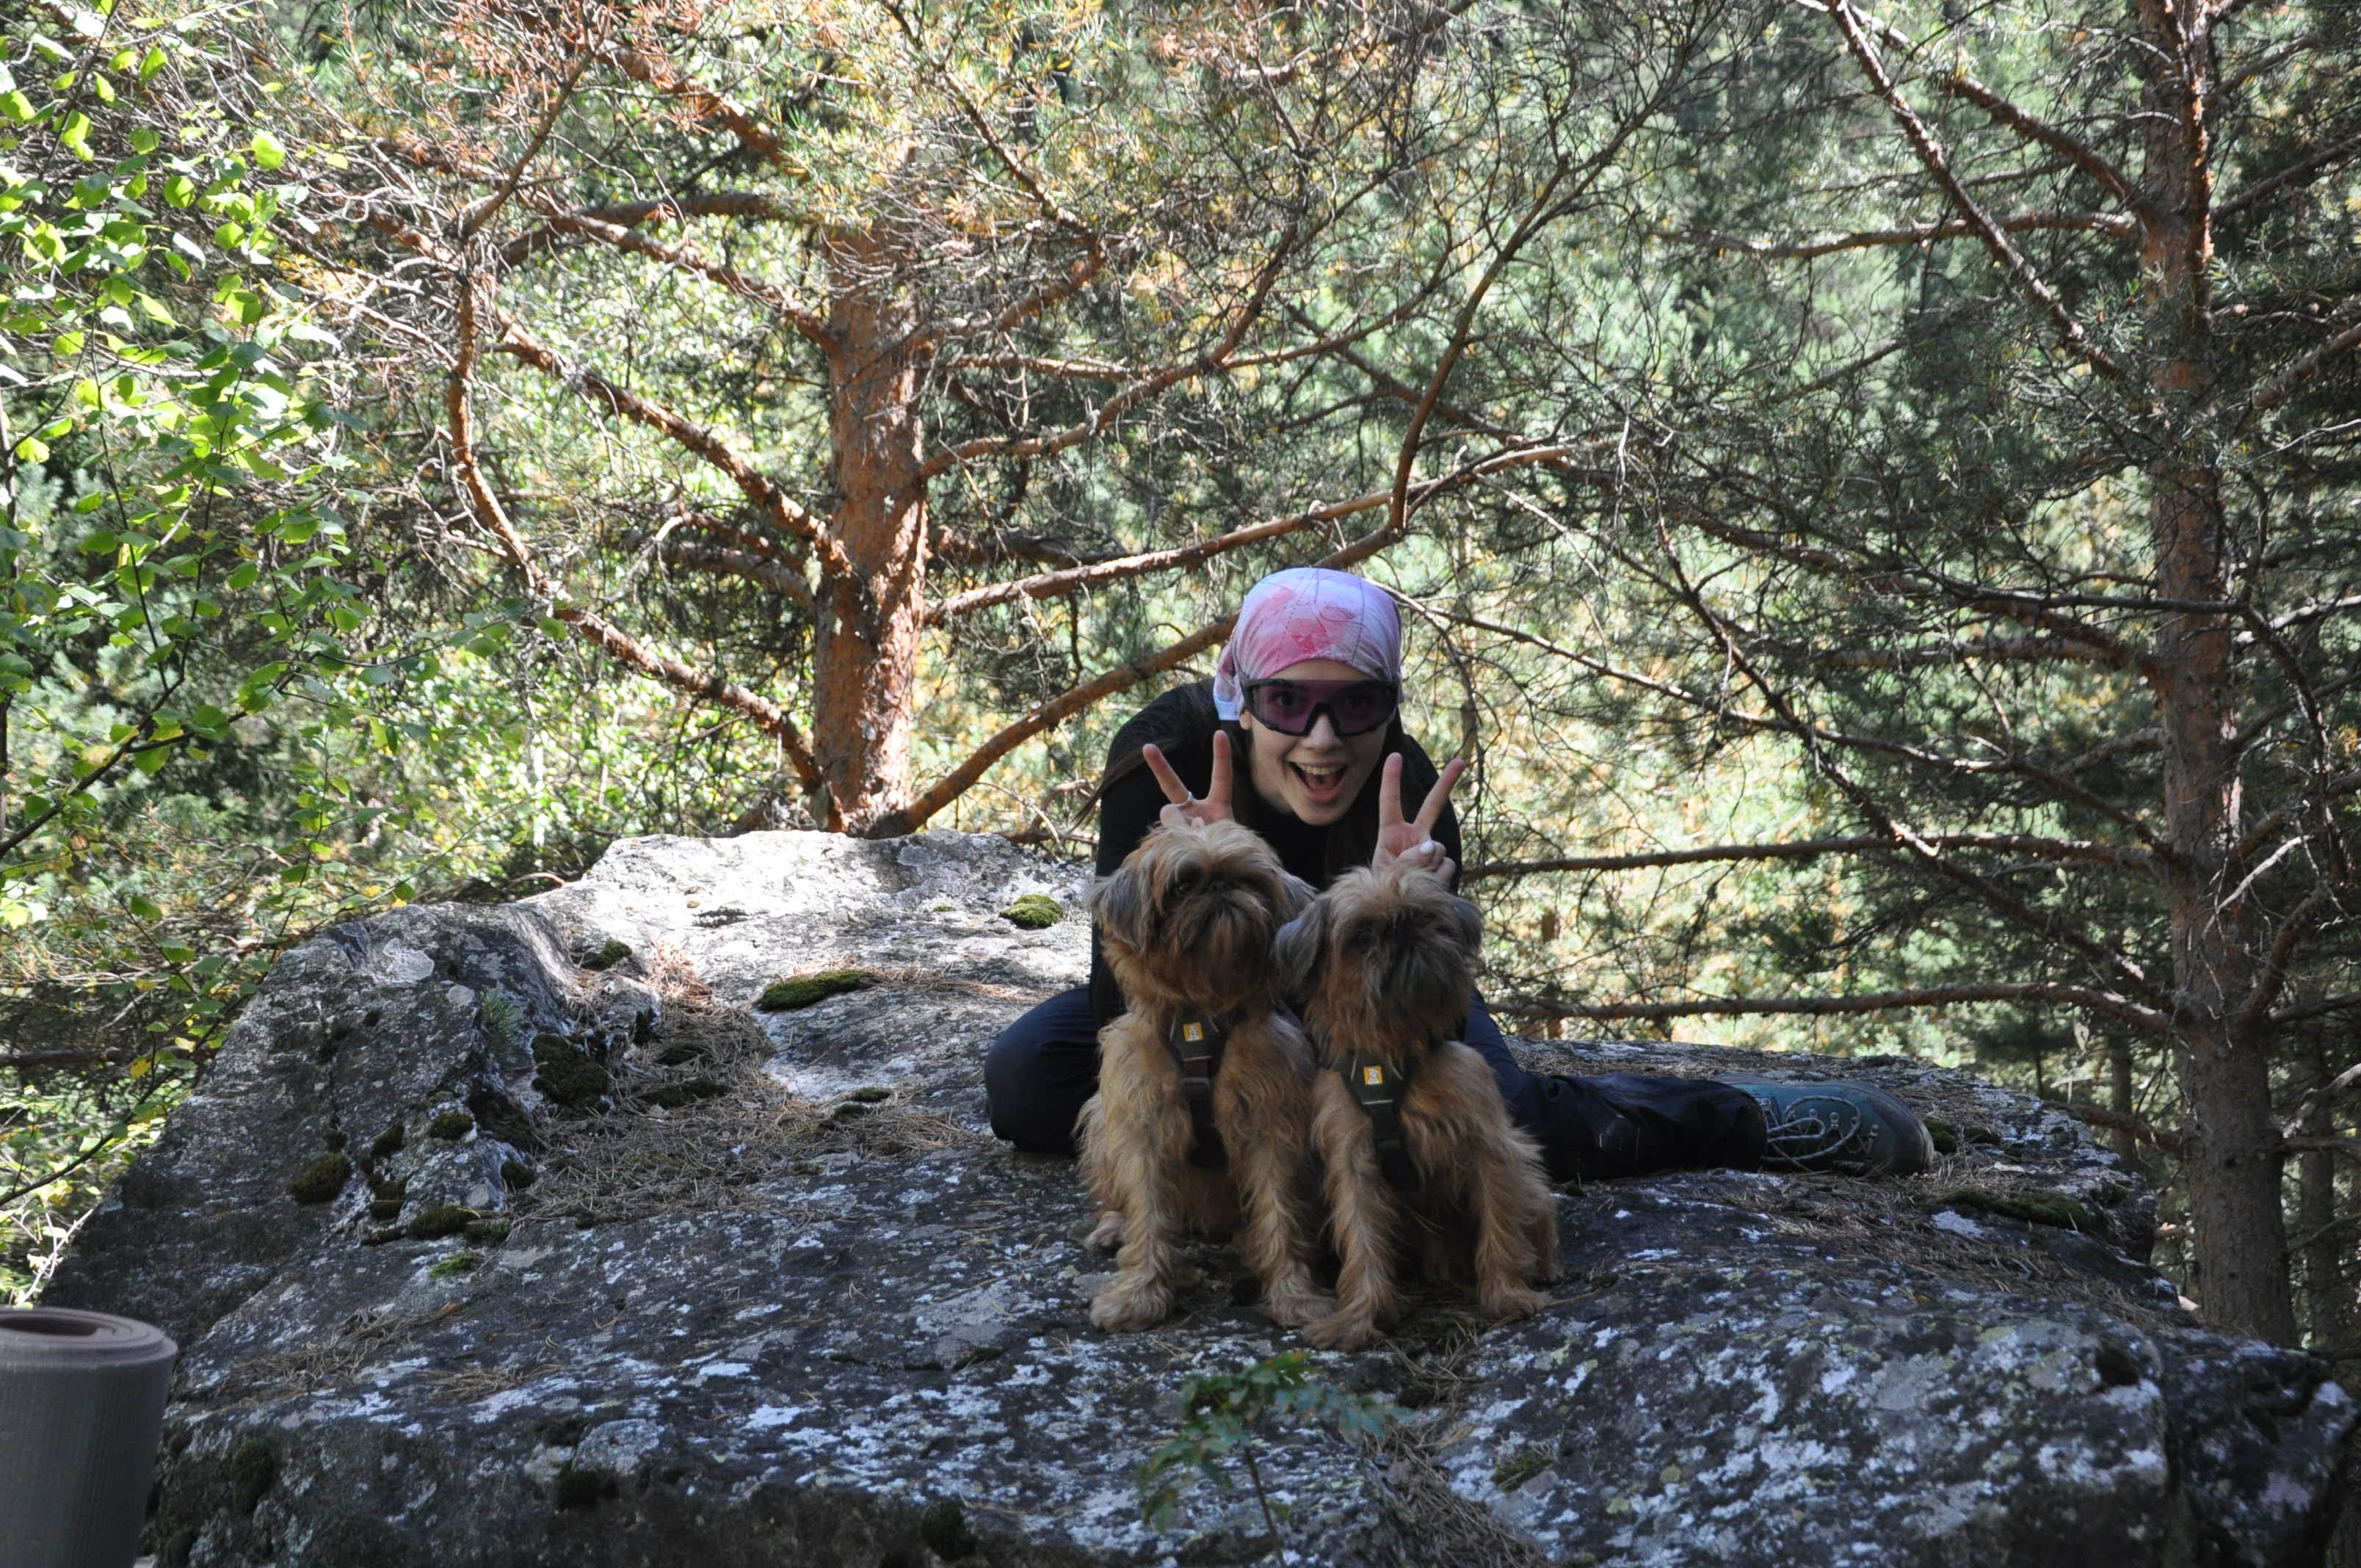
\includegraphics[width=\textwidth]{../pics/DSC_0475}			
%
%		\end{minipage}
%		\hfill
%
%	}
\end{frame}

\begin{frame}
	\frametitle{д.р. Кичкинакол Уллукёльский}
	\framesubtitle{День 1, 18 августа}
	\centering
	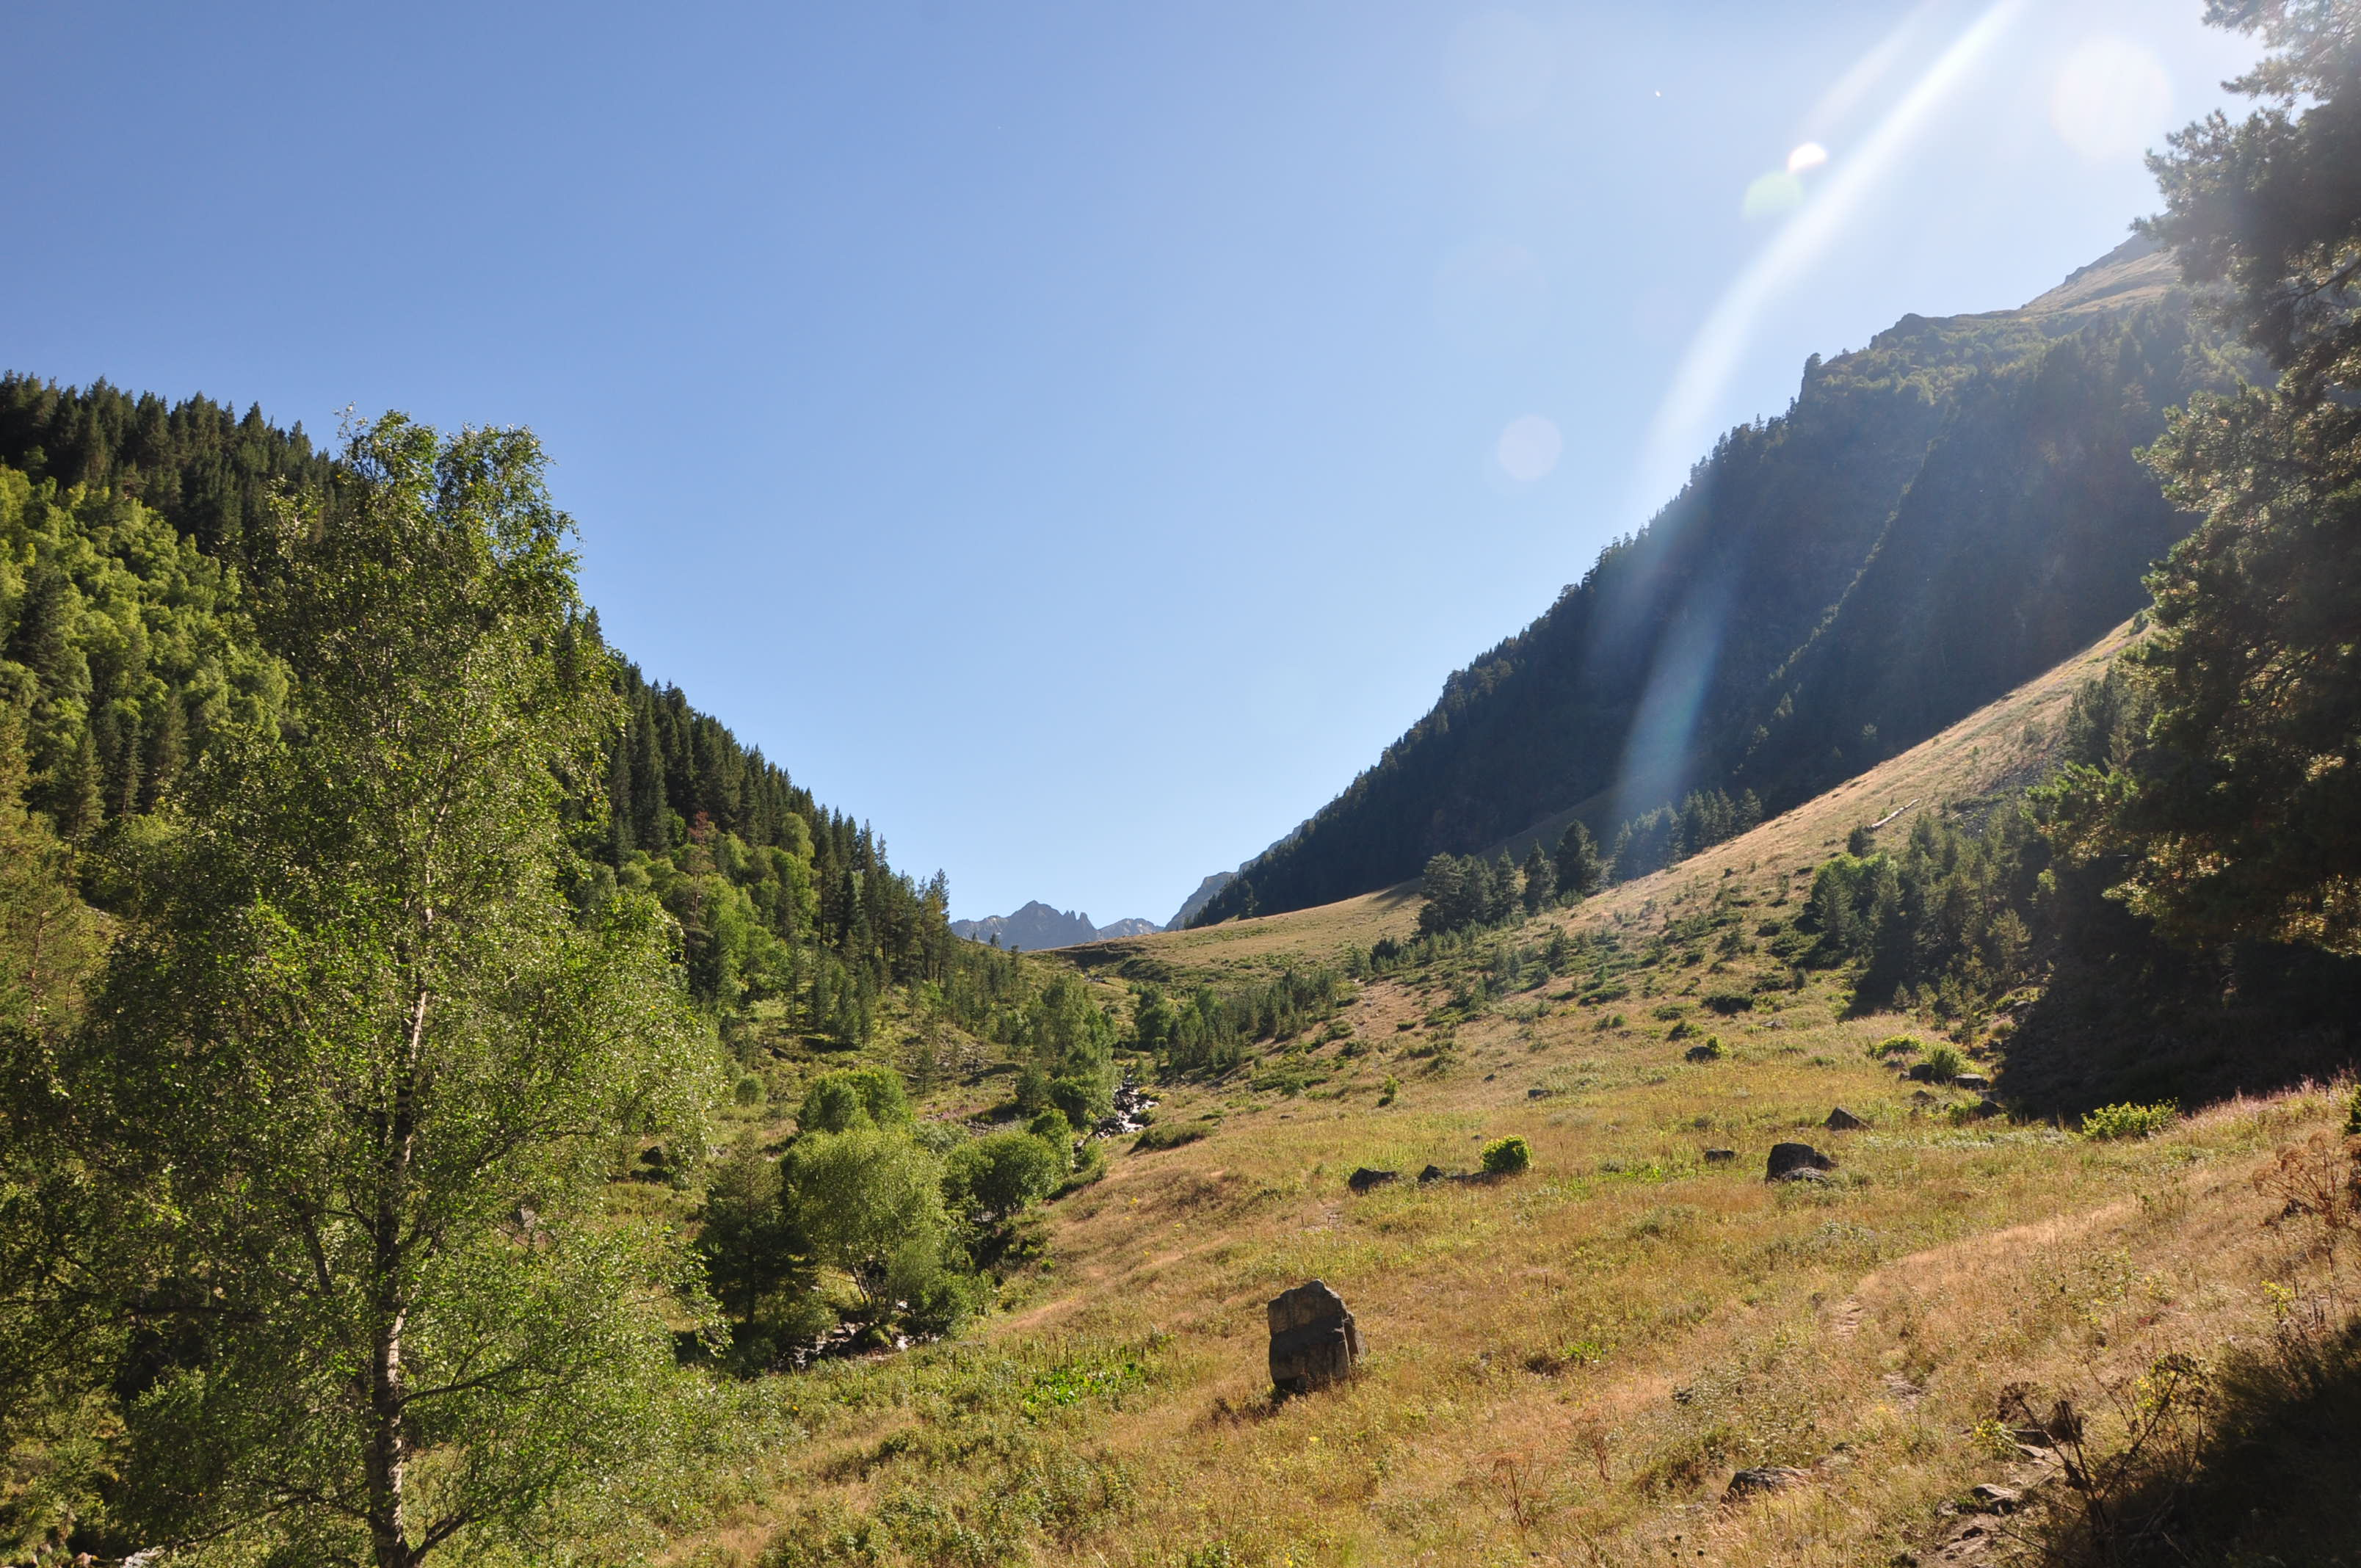
\includegraphics[width=\linewidth]{../pics/DSC_0528}
\end{frame}

\begin{frame}
	\frametitle{Крокусы}
	\framesubtitle{День 1, 18 августа}
	\centering
	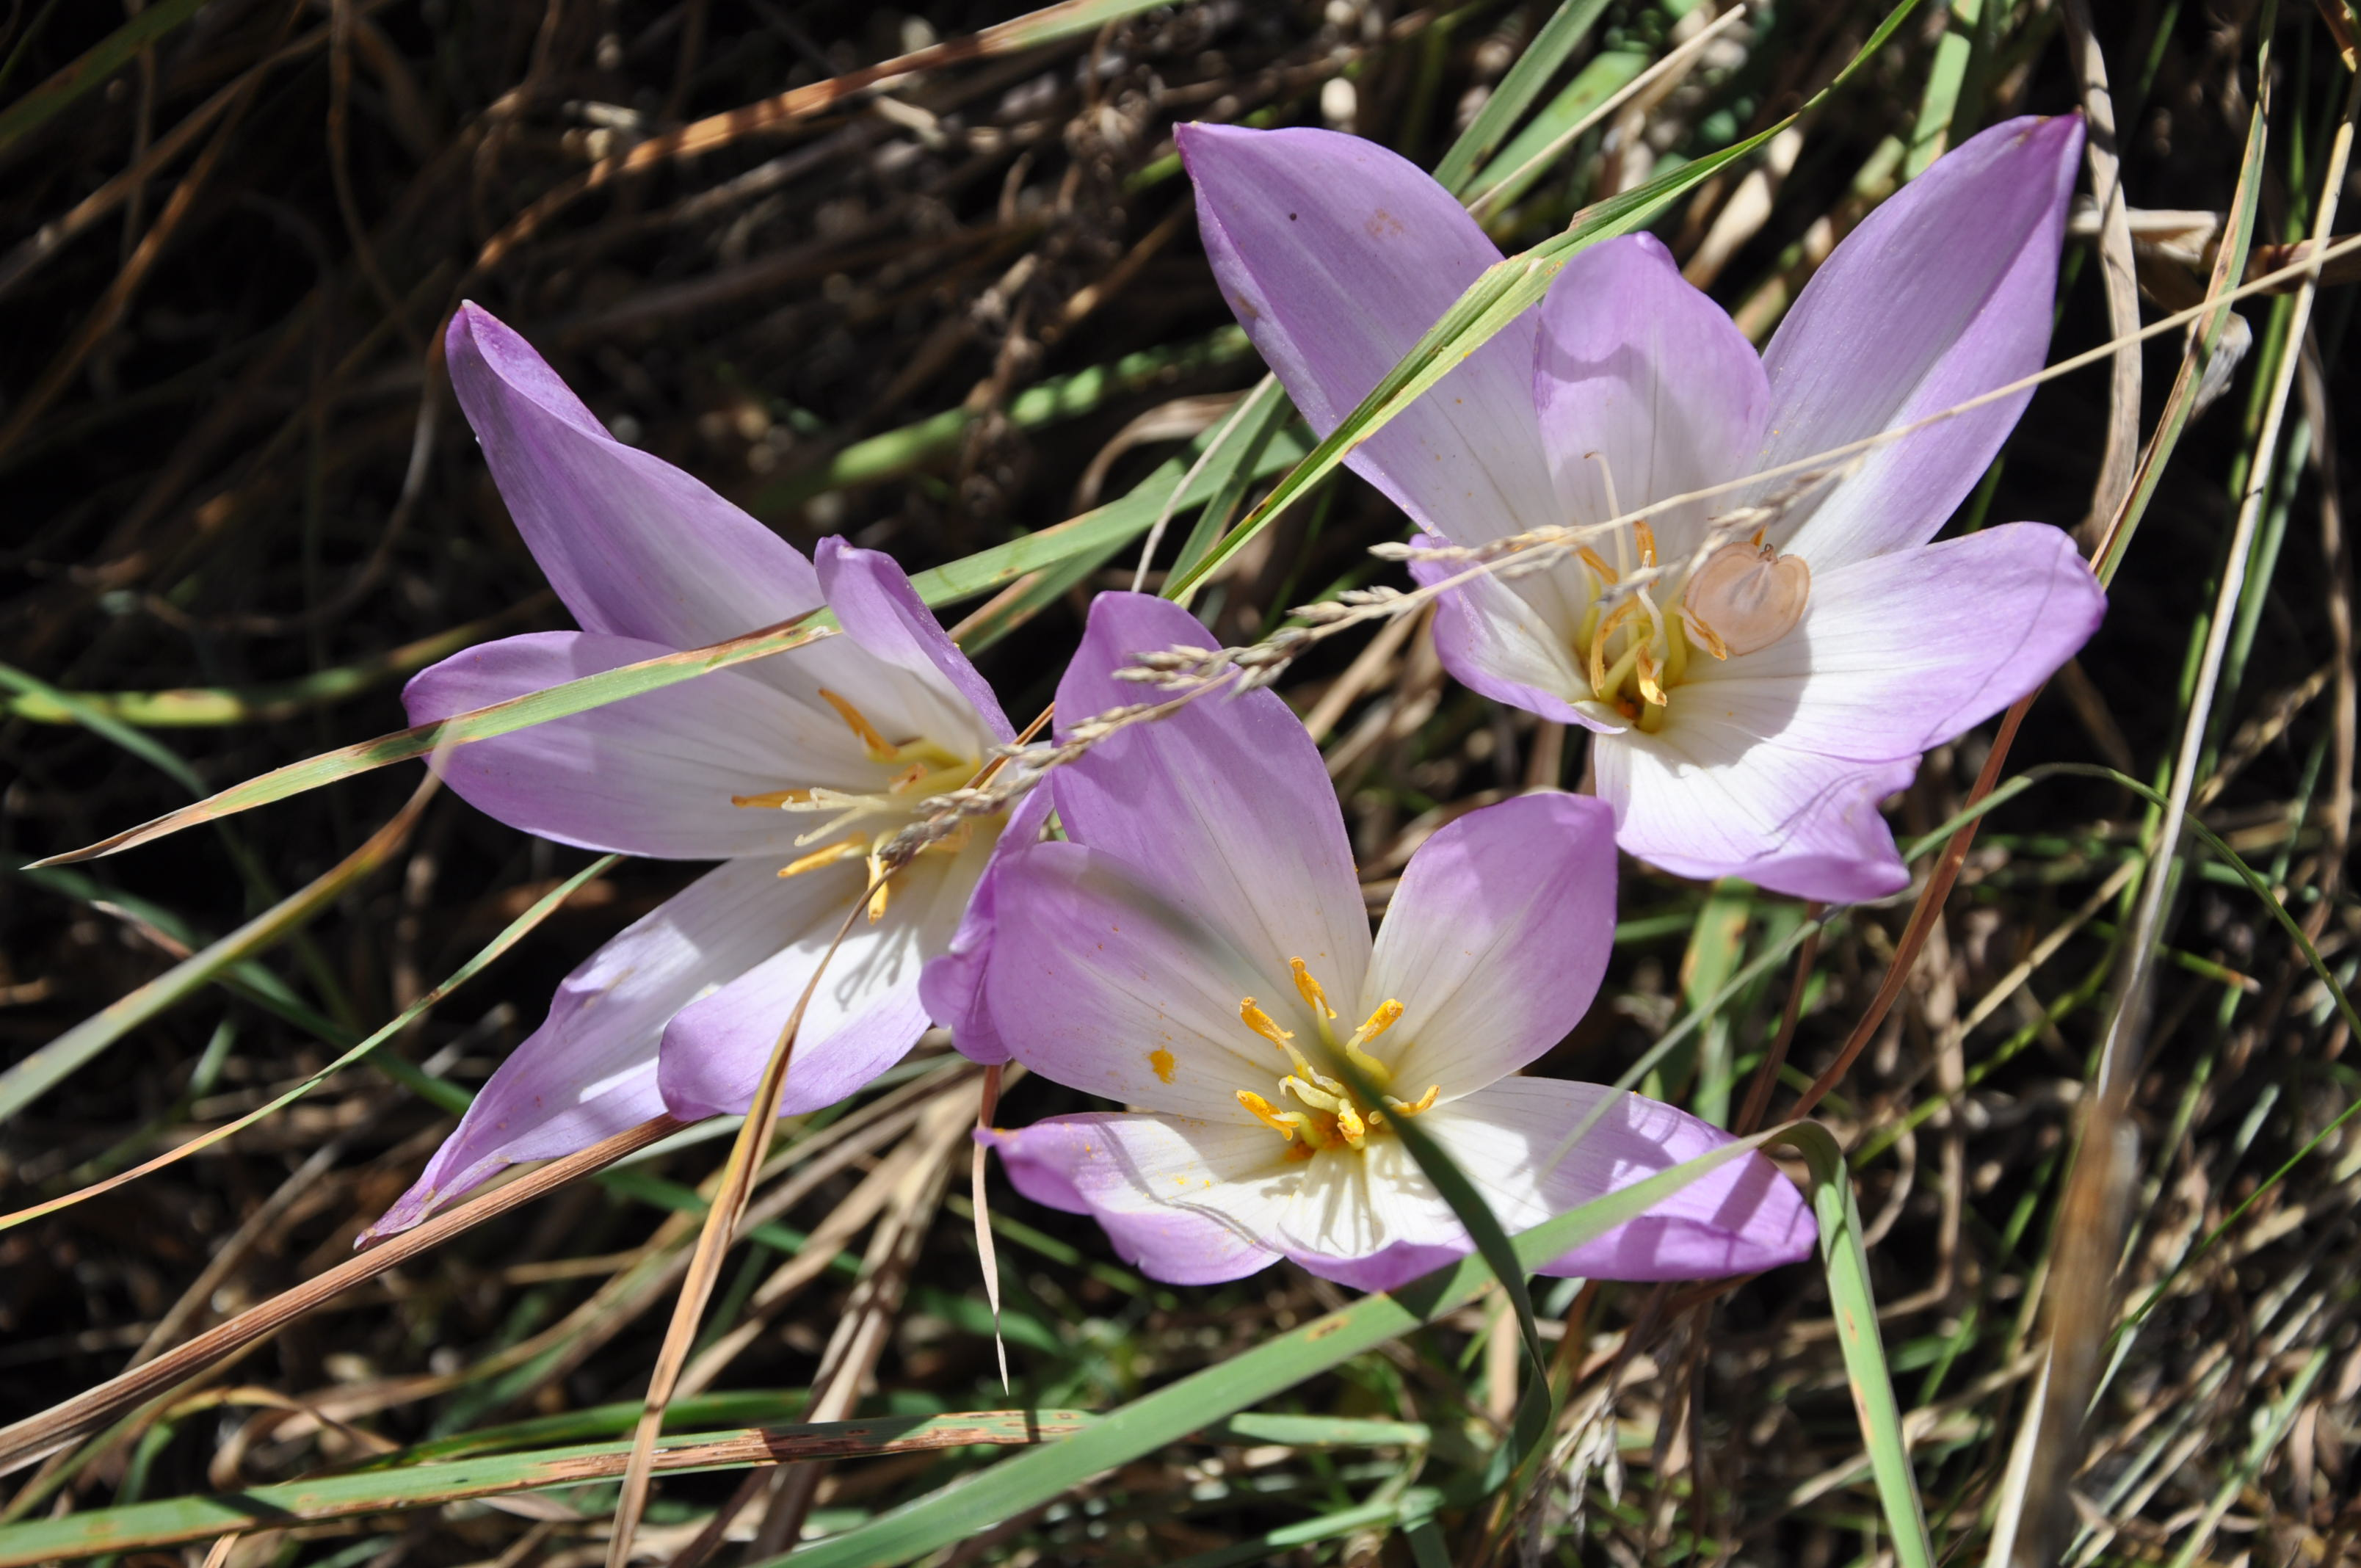
\includegraphics[width=\linewidth]{../pics/DSC_0534}
\end{frame}

\begin{frame}
	\frametitle{Реклама спальника}
	\framesubtitle{День 1, 18 августа}
	\centering
	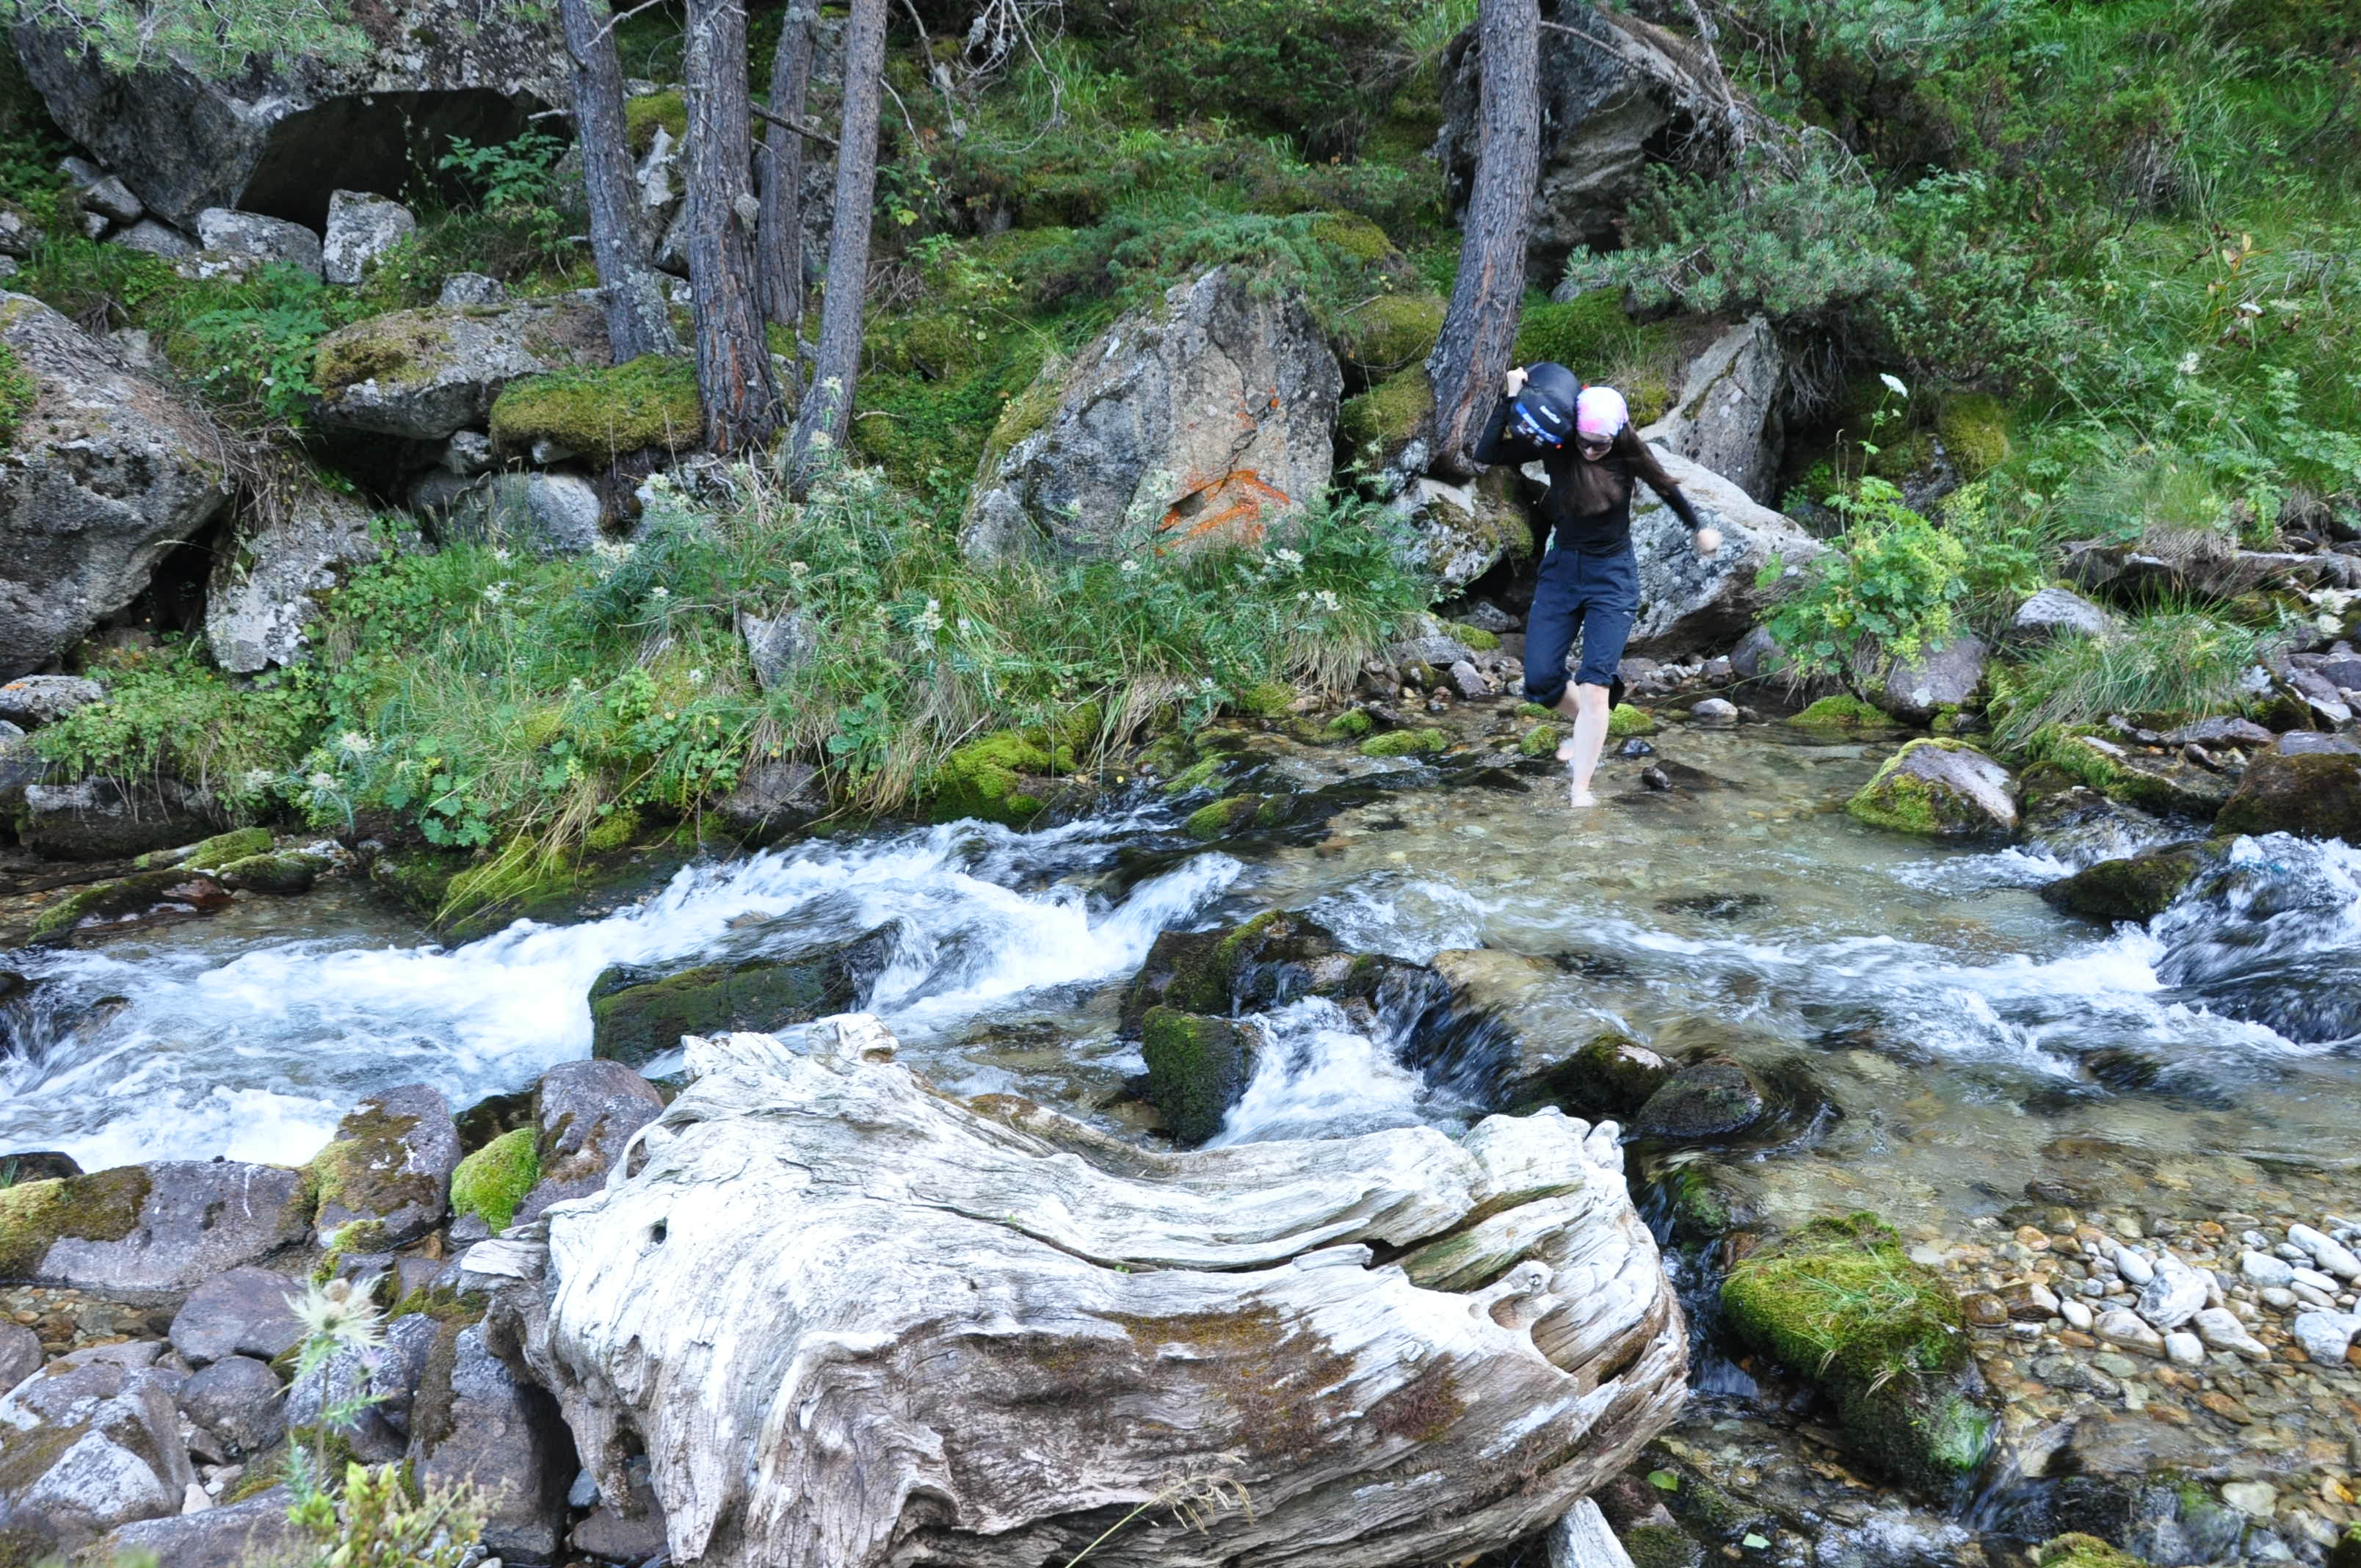
\includegraphics[width=\linewidth]{../pics/DSC_0550}
\end{frame}

\begin{frame}
	\frametitle{д.р. Кичкинакол Уллукёльский}
	\framesubtitle{День 1, 18 августа}
	«Кичкине къол»~--- «Маленькое ущелье»
	\centering
	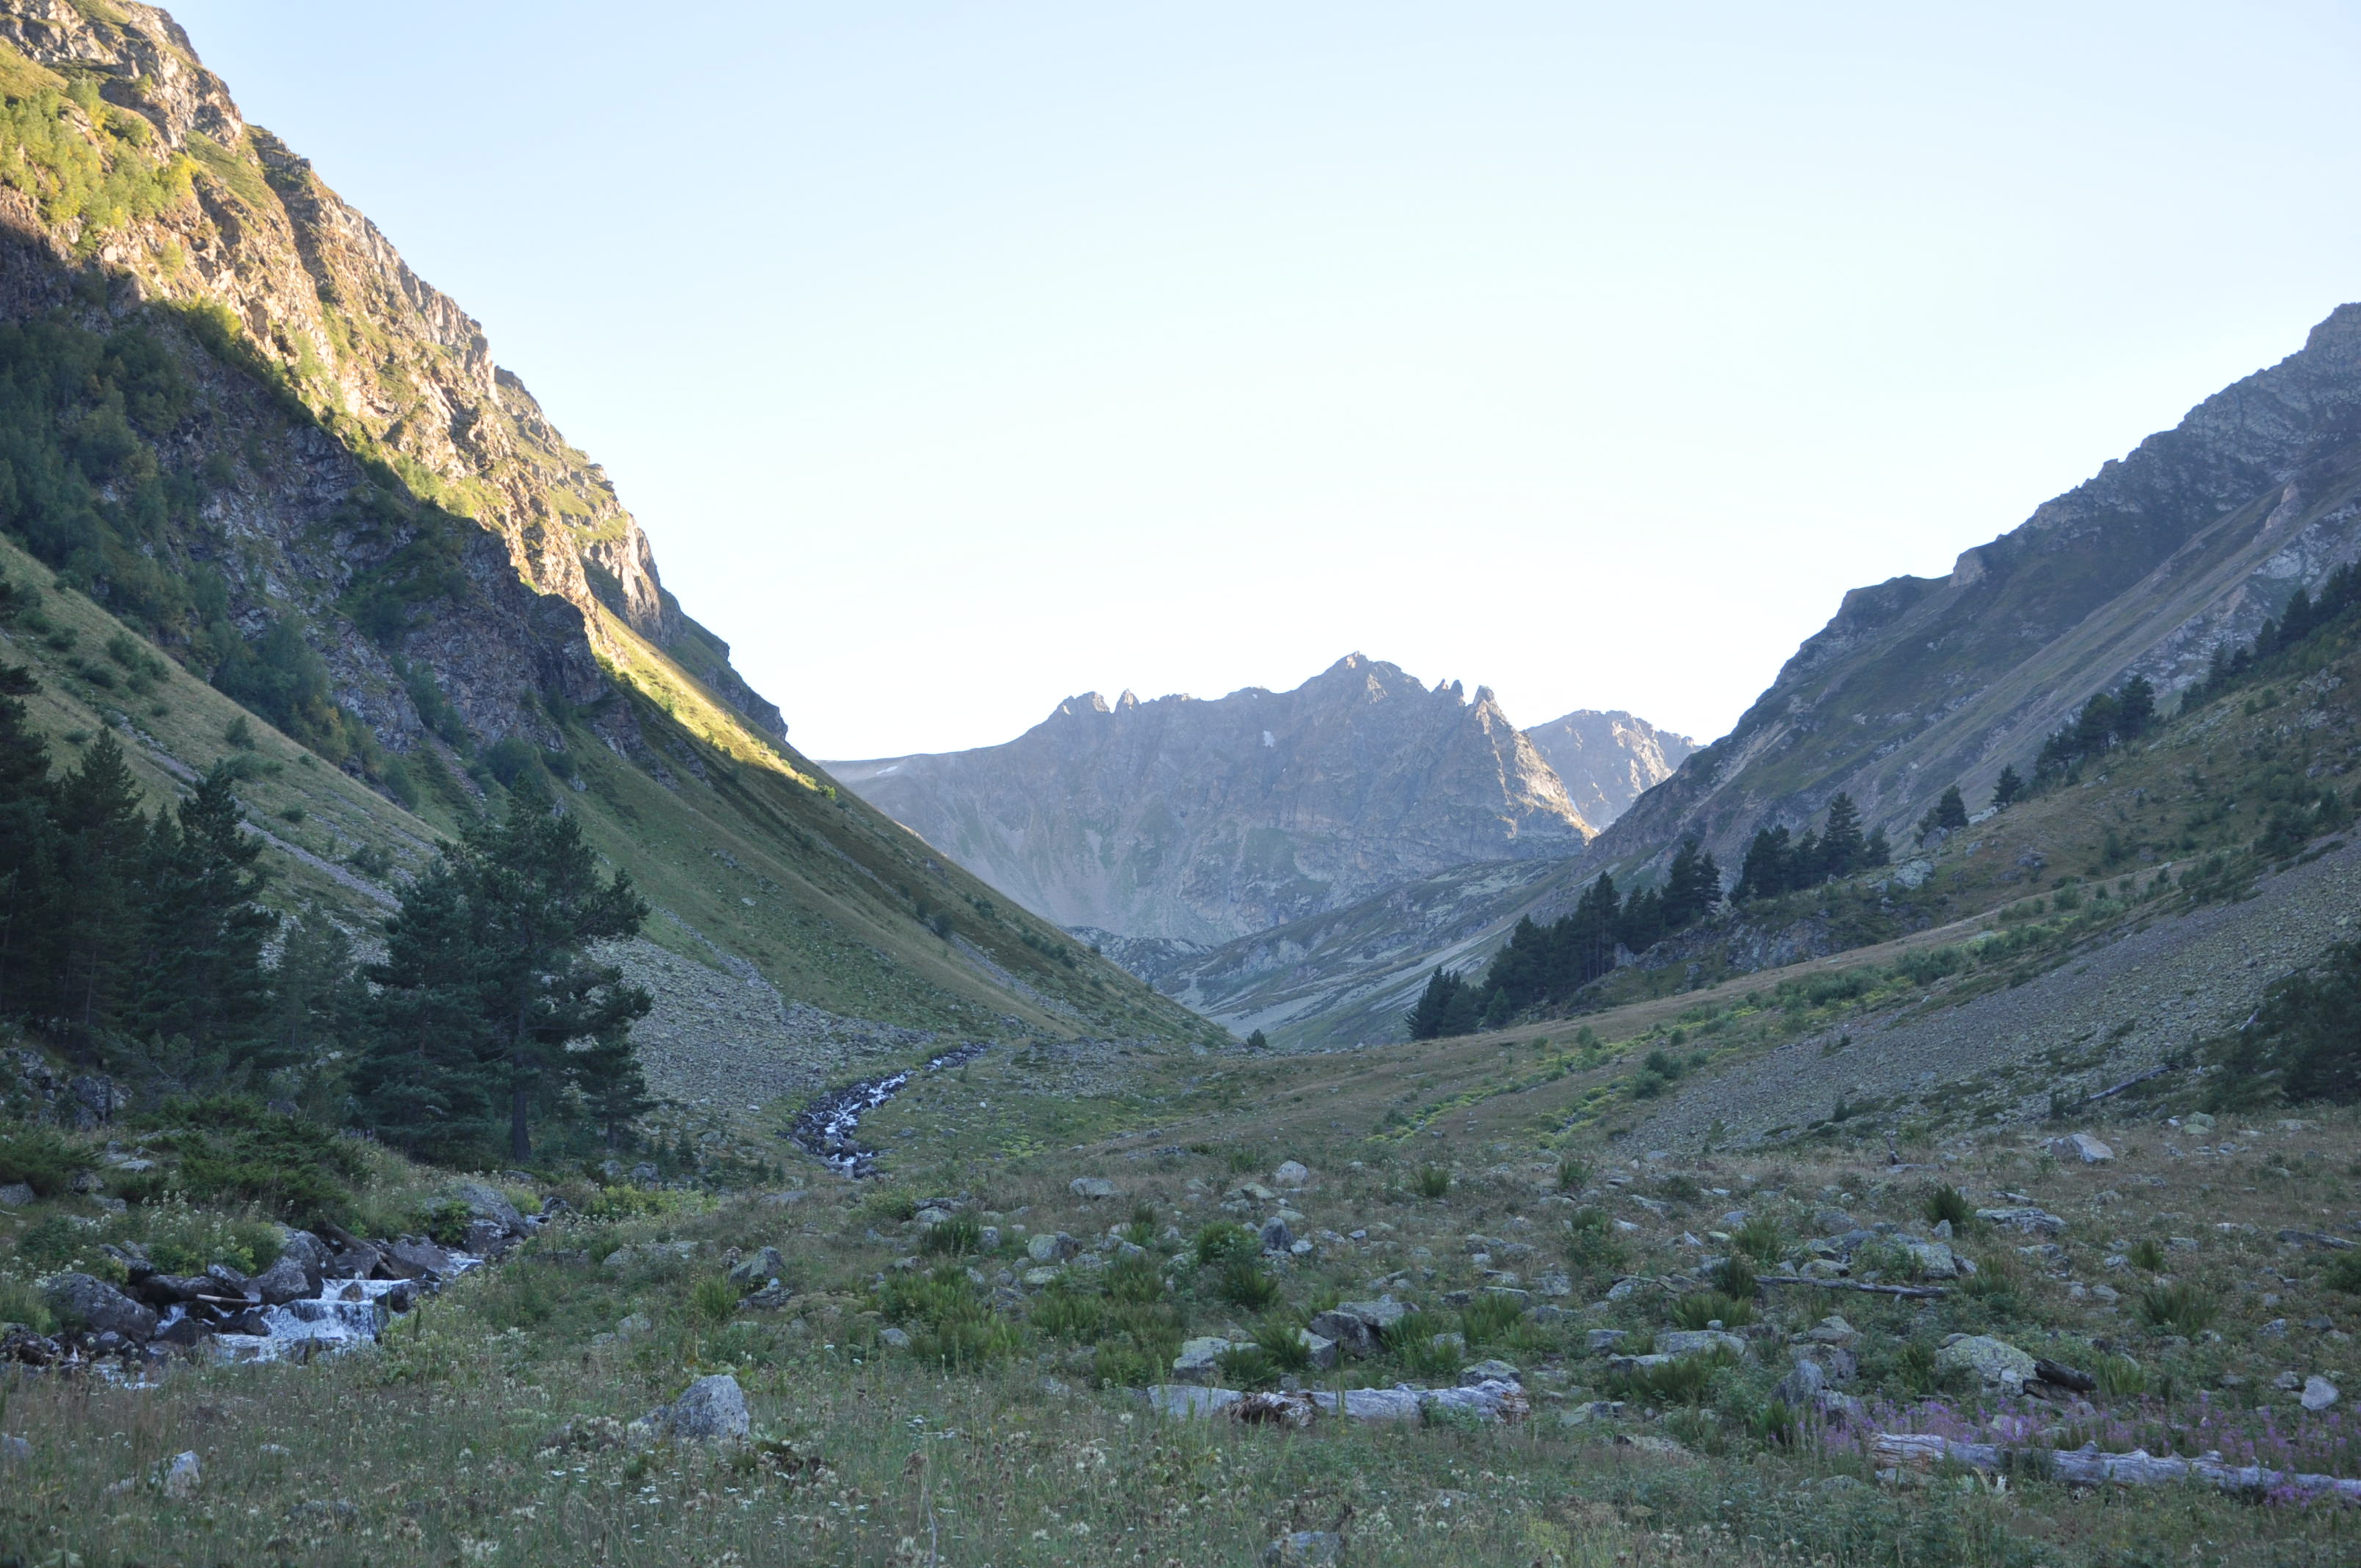
\includegraphics[width=\linewidth]{../pics/DSC_0558}
\end{frame}

\begin{frame}
	\frametitle{Чешем к м.н.}
	\framesubtitle{День 1, 18 августа}
	\centering
	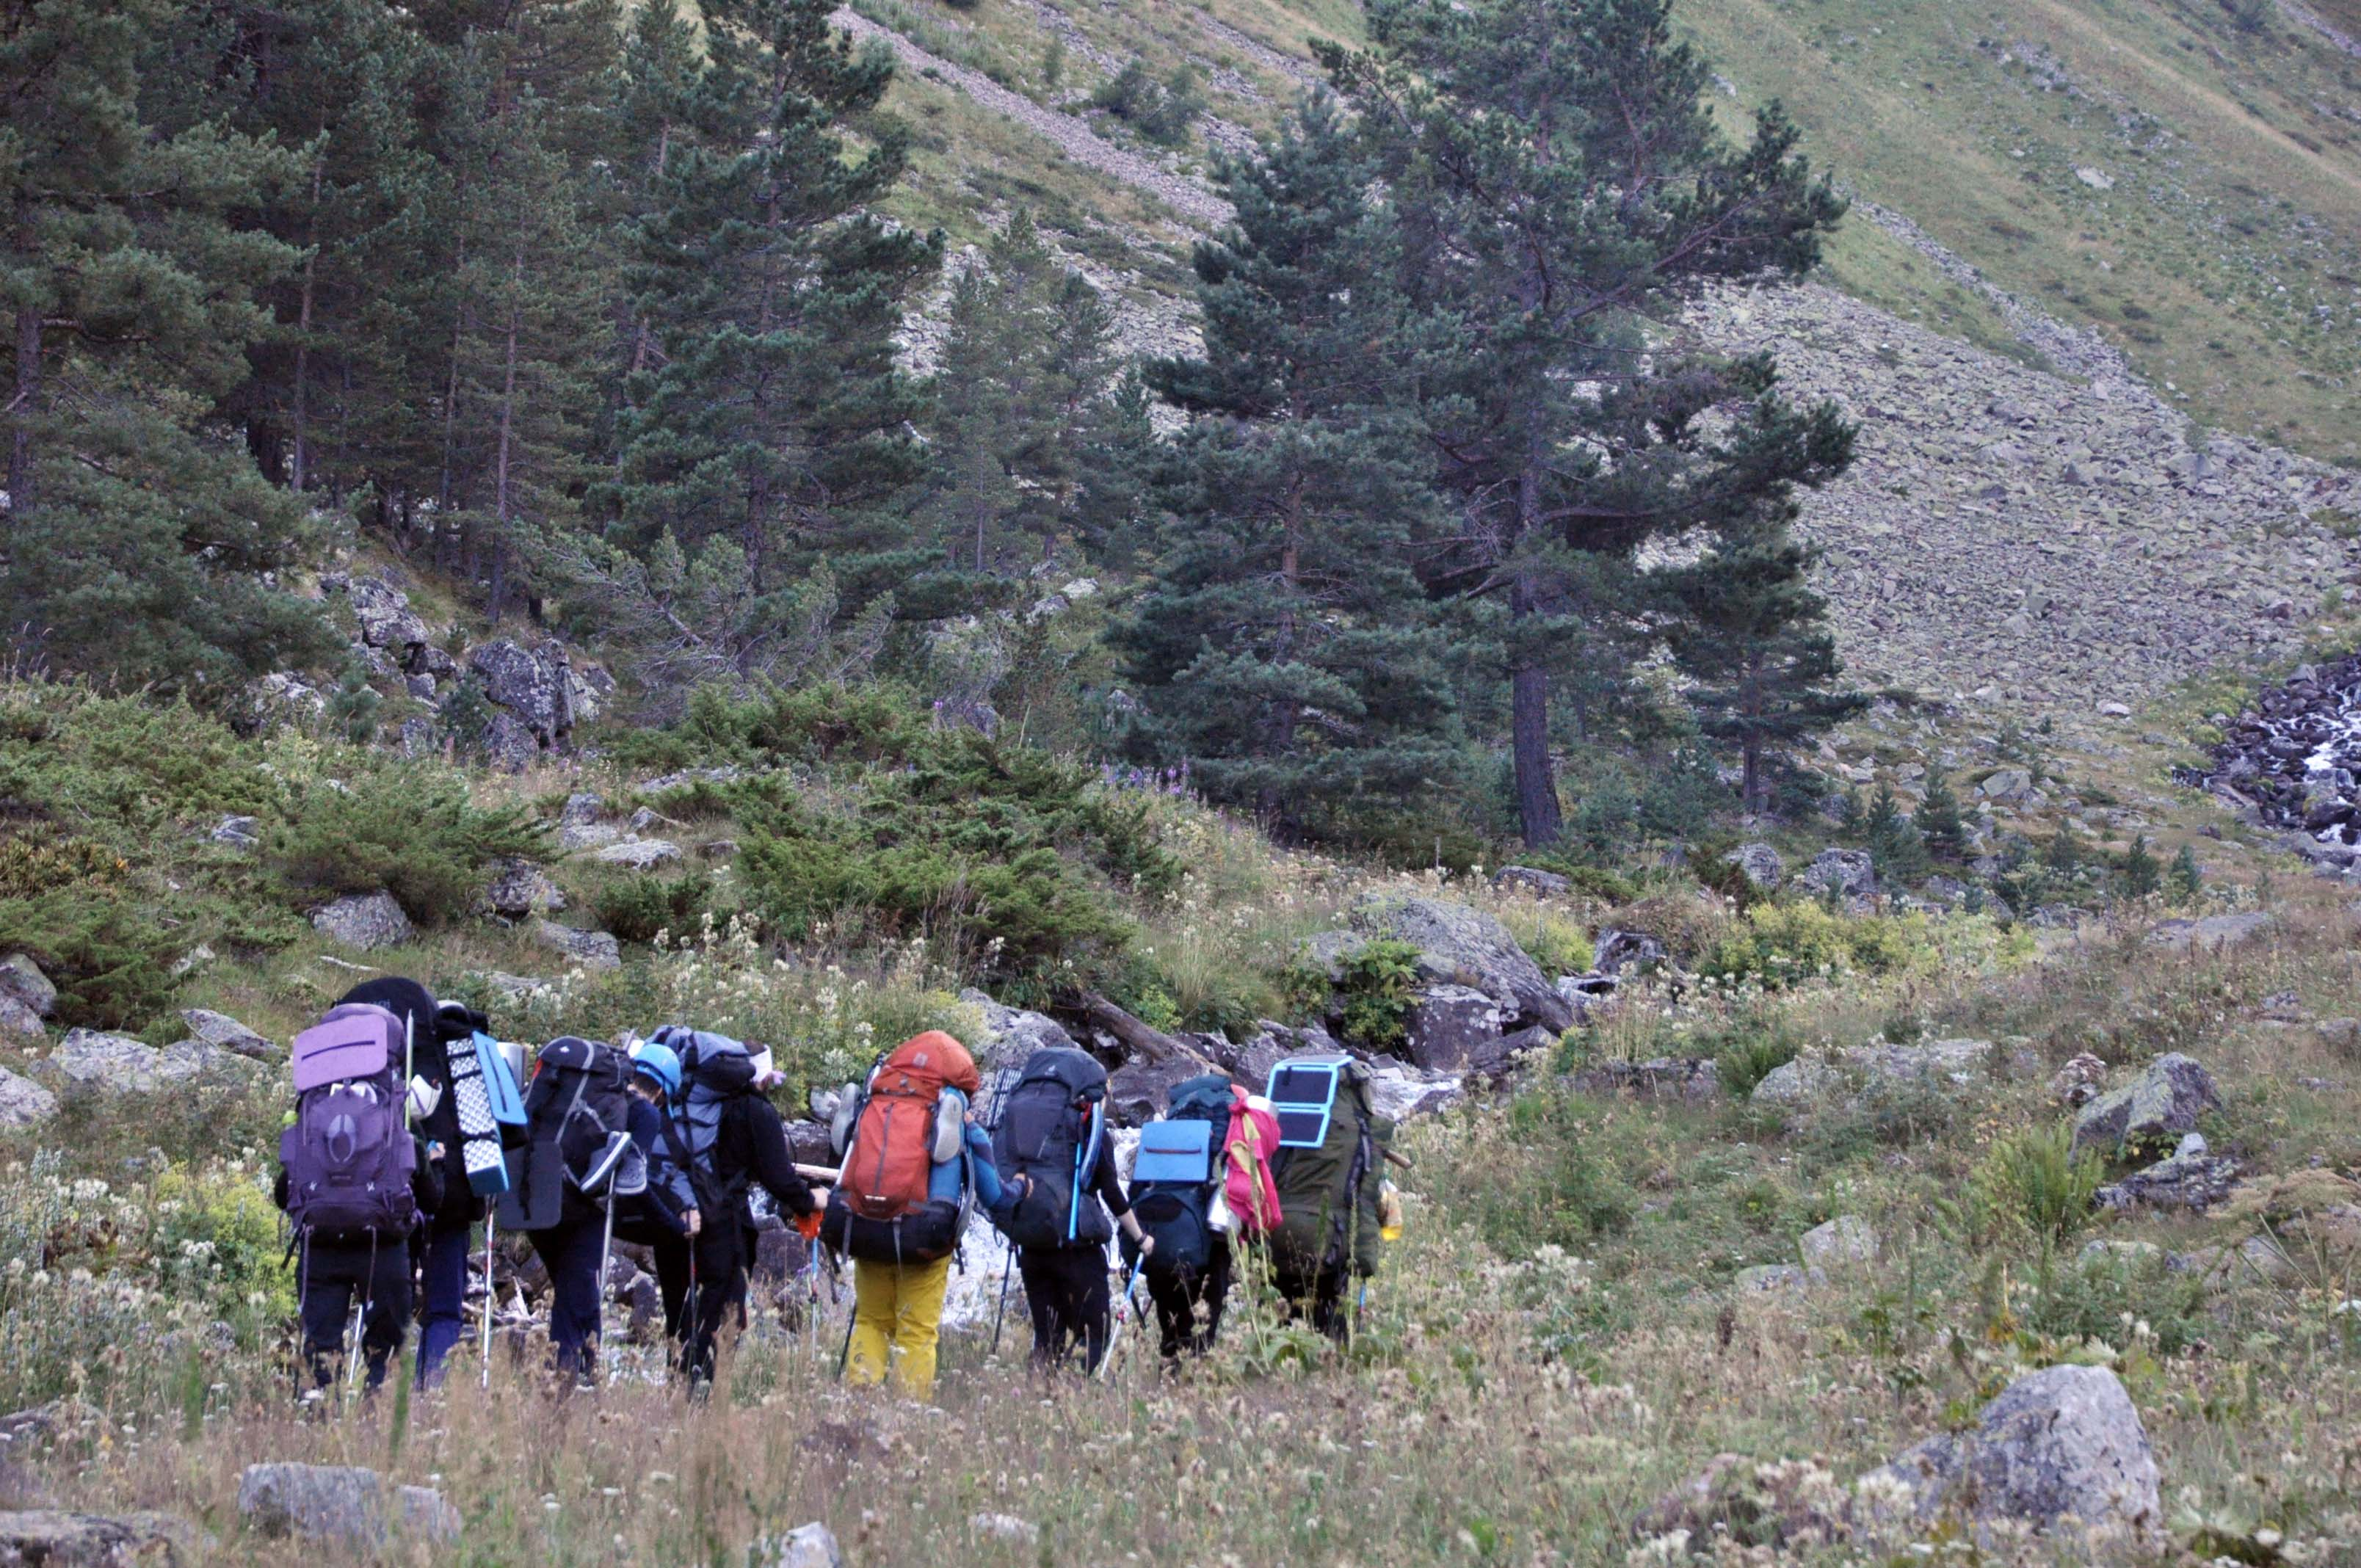
\includegraphics[width=\linewidth]{../pics/DSC_0559}
\end{frame}

\begin{frame}
	\frametitle{д.р. Кичкинакол Уллукёльский}
	\framesubtitle{День 1, 18 августа}
	\centering
	\rotatebox{90}{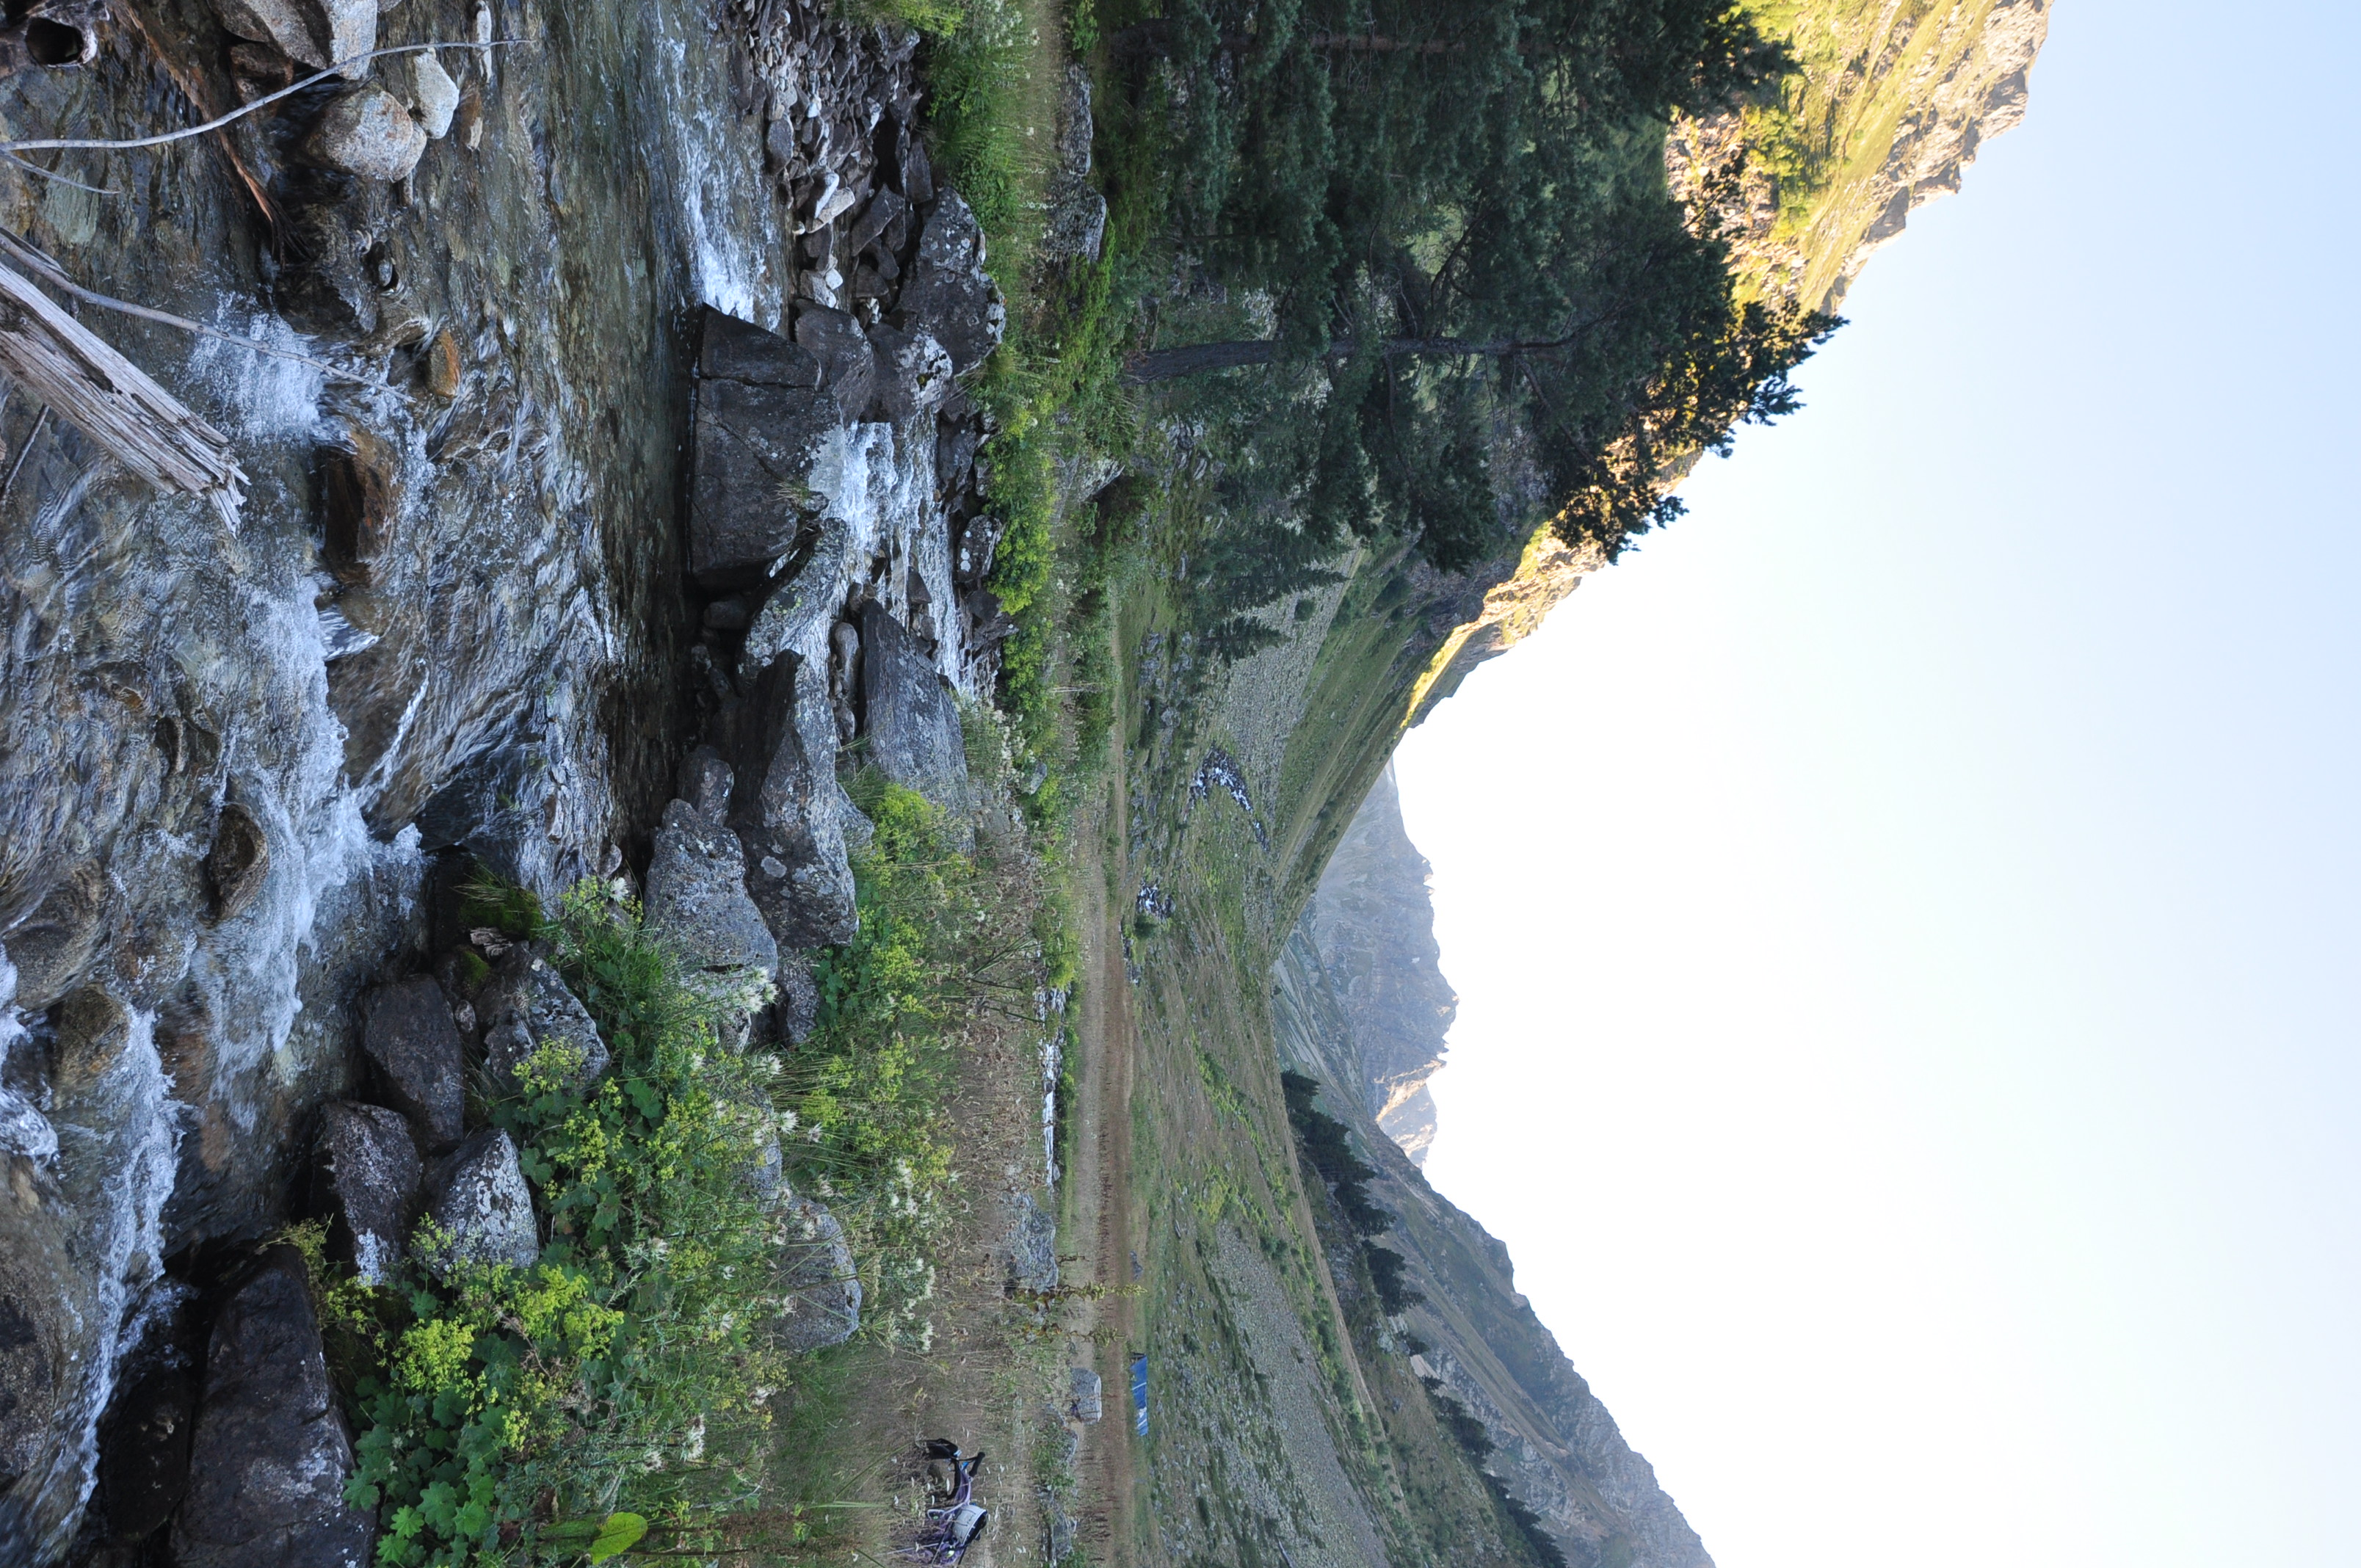
\includegraphics[width=0.67\linewidth]{../pics/DSC_0563}}
\end{frame}

\begin{frame}
	\frametitle{Горечавковое}
	\framesubtitle{День 1, 18 августа}
	\centering
	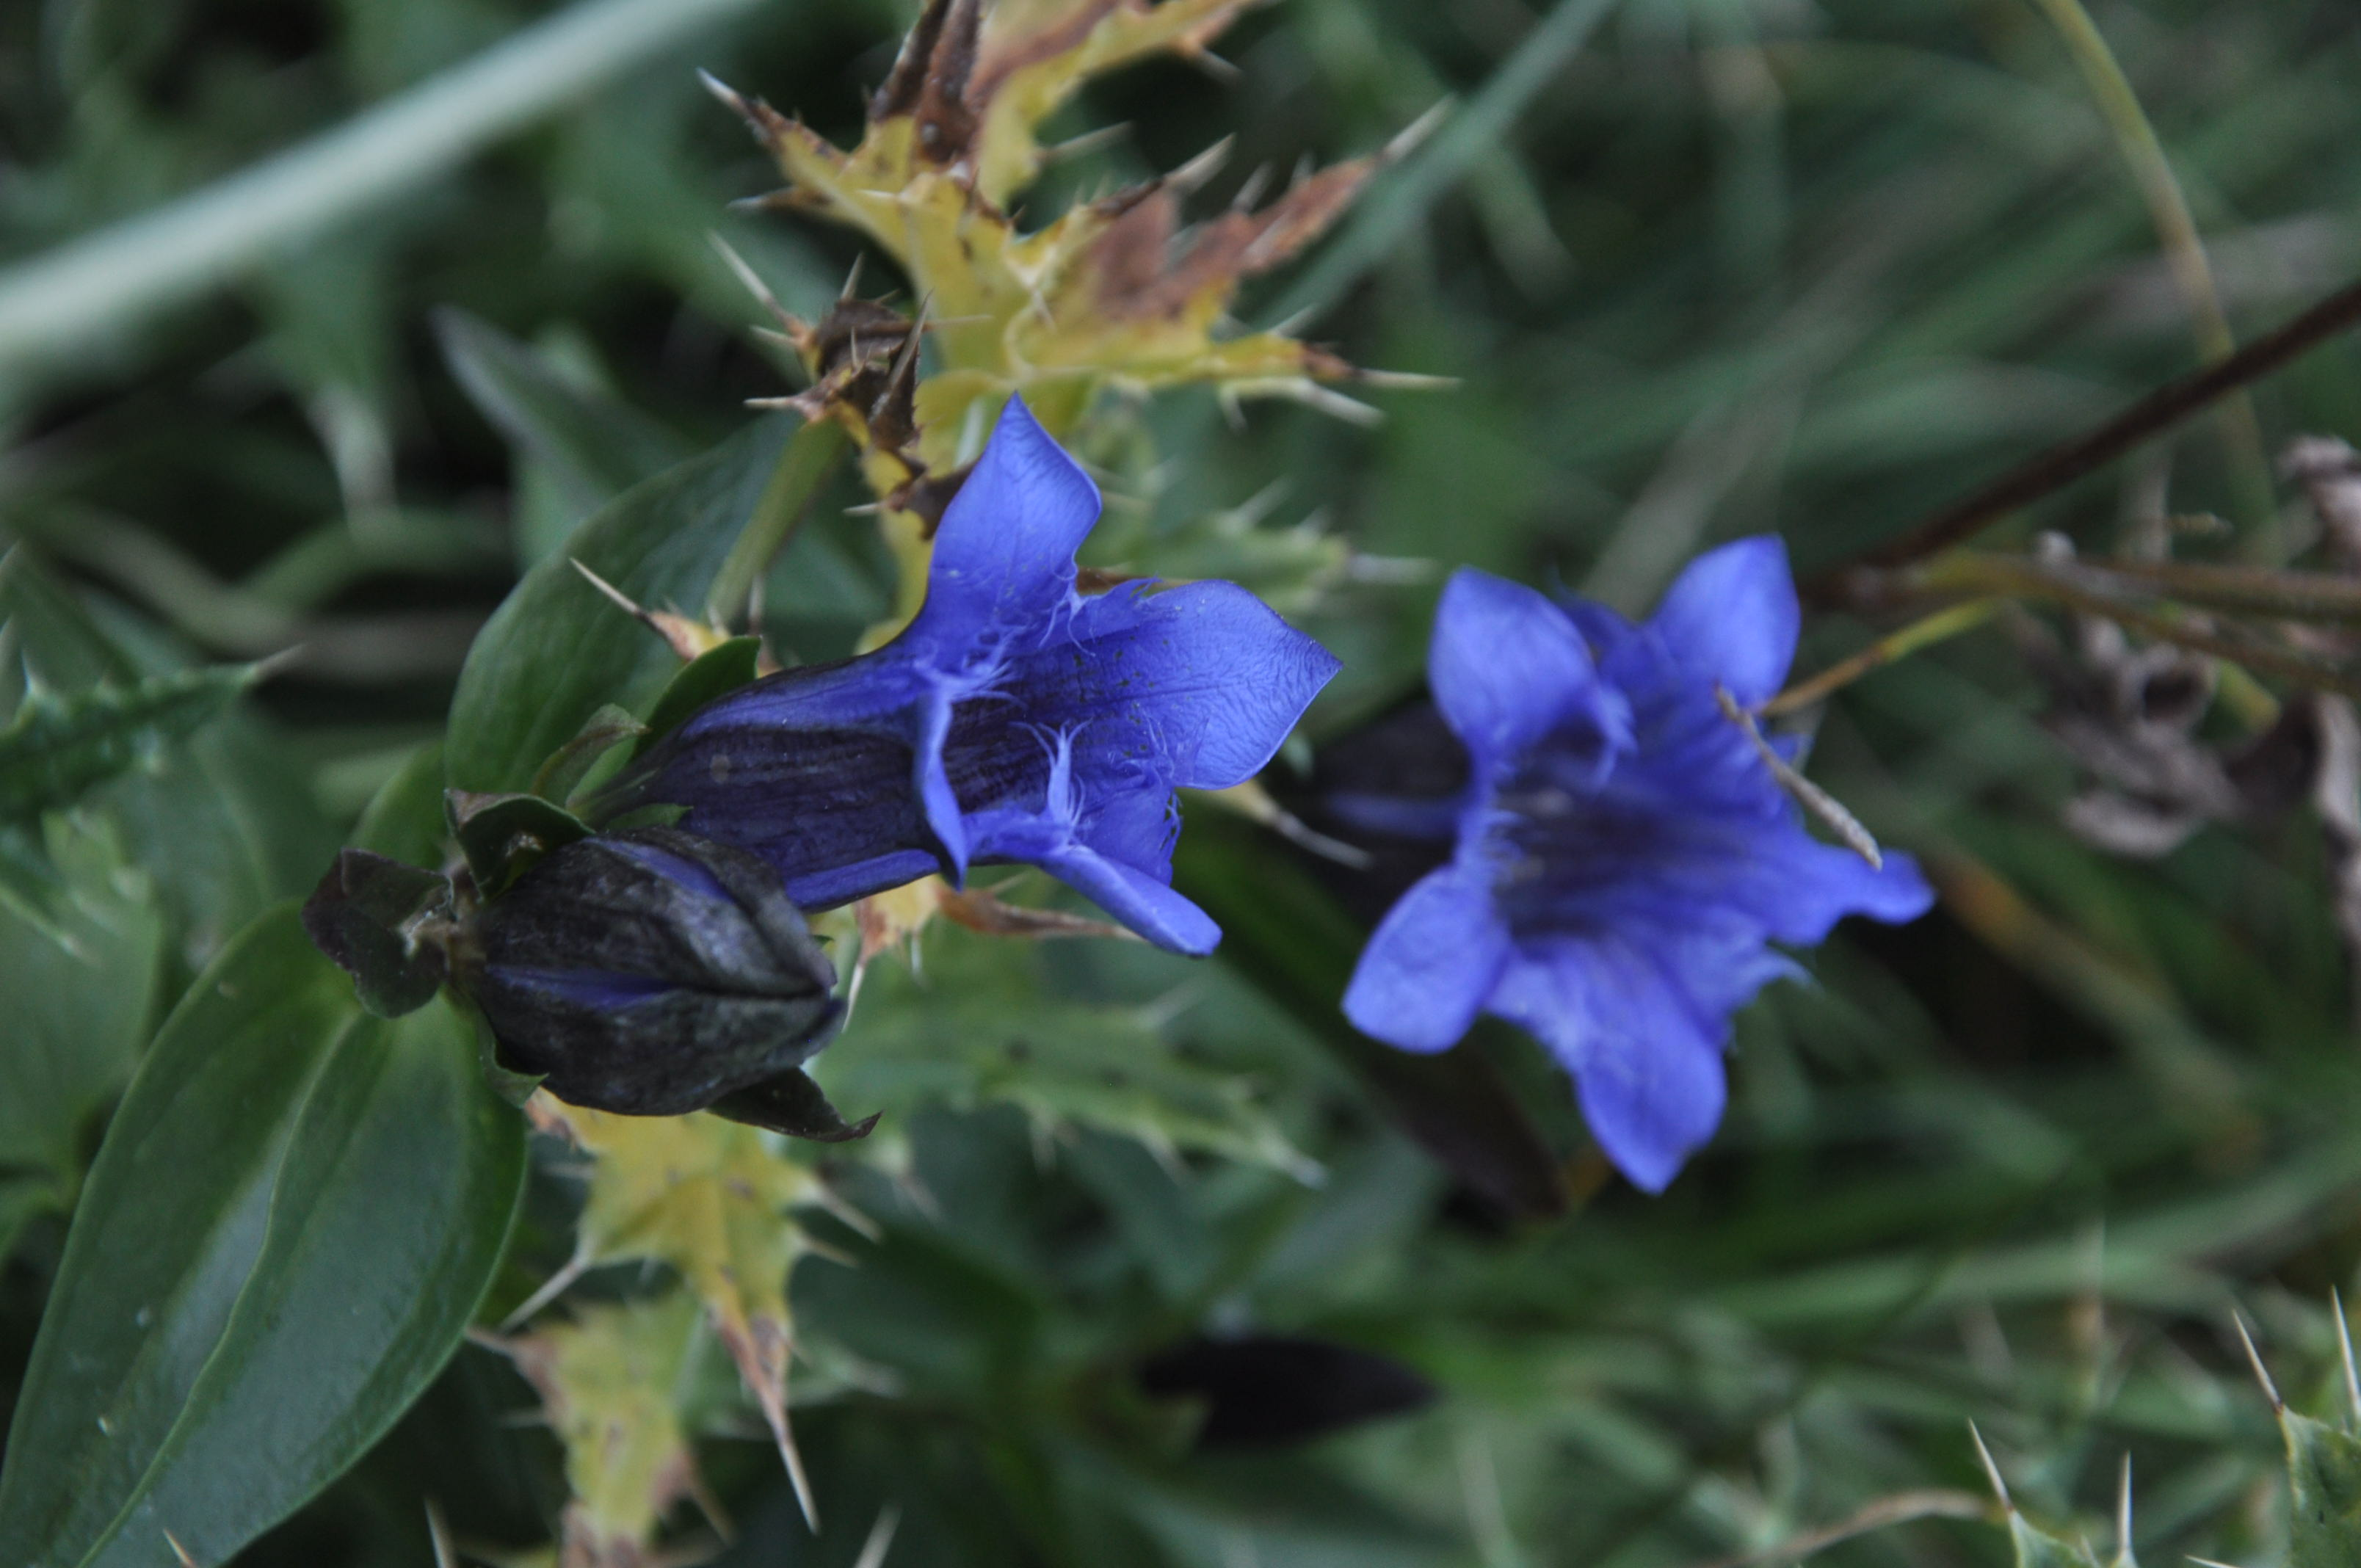
\includegraphics[width=\linewidth]{../pics/DSC_0585}
\end{frame}
		\begin{frame}
	\frametitle{День 2. 19 августа}
	\framesubtitle{д.р. Кичкинакол Уллукёльский~--- оз. Гитче-Кёль~---оз. Уллу-Кёль} % Optional subtitle
	\begin{columns}[c] % The "c" option specifies centered vertical alignment while the "t" option is used for top vertical alignment
		\begin{column}{0.45\textwidth} % Left column width
			\begin{itemize}
				\item Забег по долине Кичкинакола
				\item Купание в Гитче-Кёль и думы руководы
				\item Попытки в снежные занятия
				\item ...Последнее, что видит дрон~--- это снежник Уллукёля Восточного \frownie
				\item Прошли \textbf{5.6} км
				\item ЧХВ: 3:25
				\item Набор/сброс: \textcolor{darkred}{\textbf{+650}}/\textcolor{darkblue}{\textbf{-0}}~м
			\end{itemize}
			
		\end{column}
		\begin{column}{0.5\textwidth} % Right column width
			\centering
			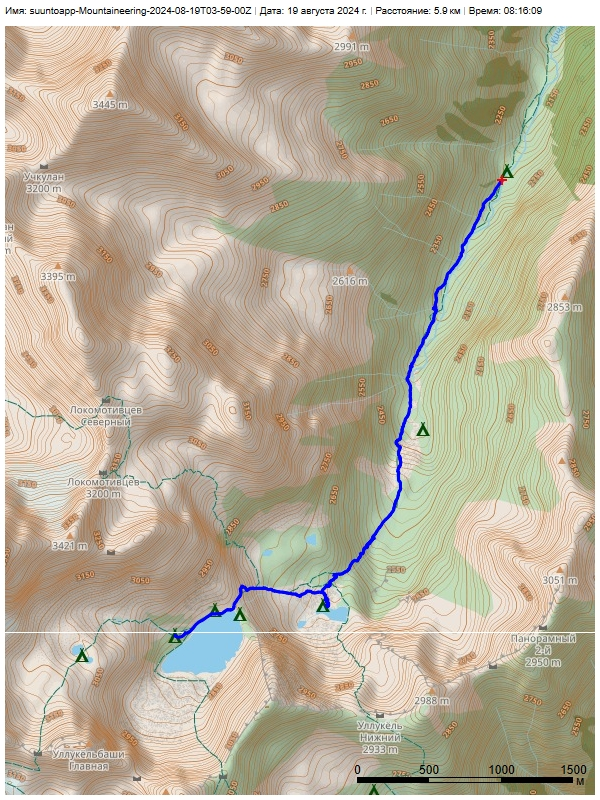
\includegraphics[width=\linewidth]{../pics/mini_maps/19}
		\end{column}
	\end{columns}
\end{frame}

\begin{frame}
	\frametitle{Подъём по древней морене}
	\framesubtitle{День 2, 19 августа}
	\centering
	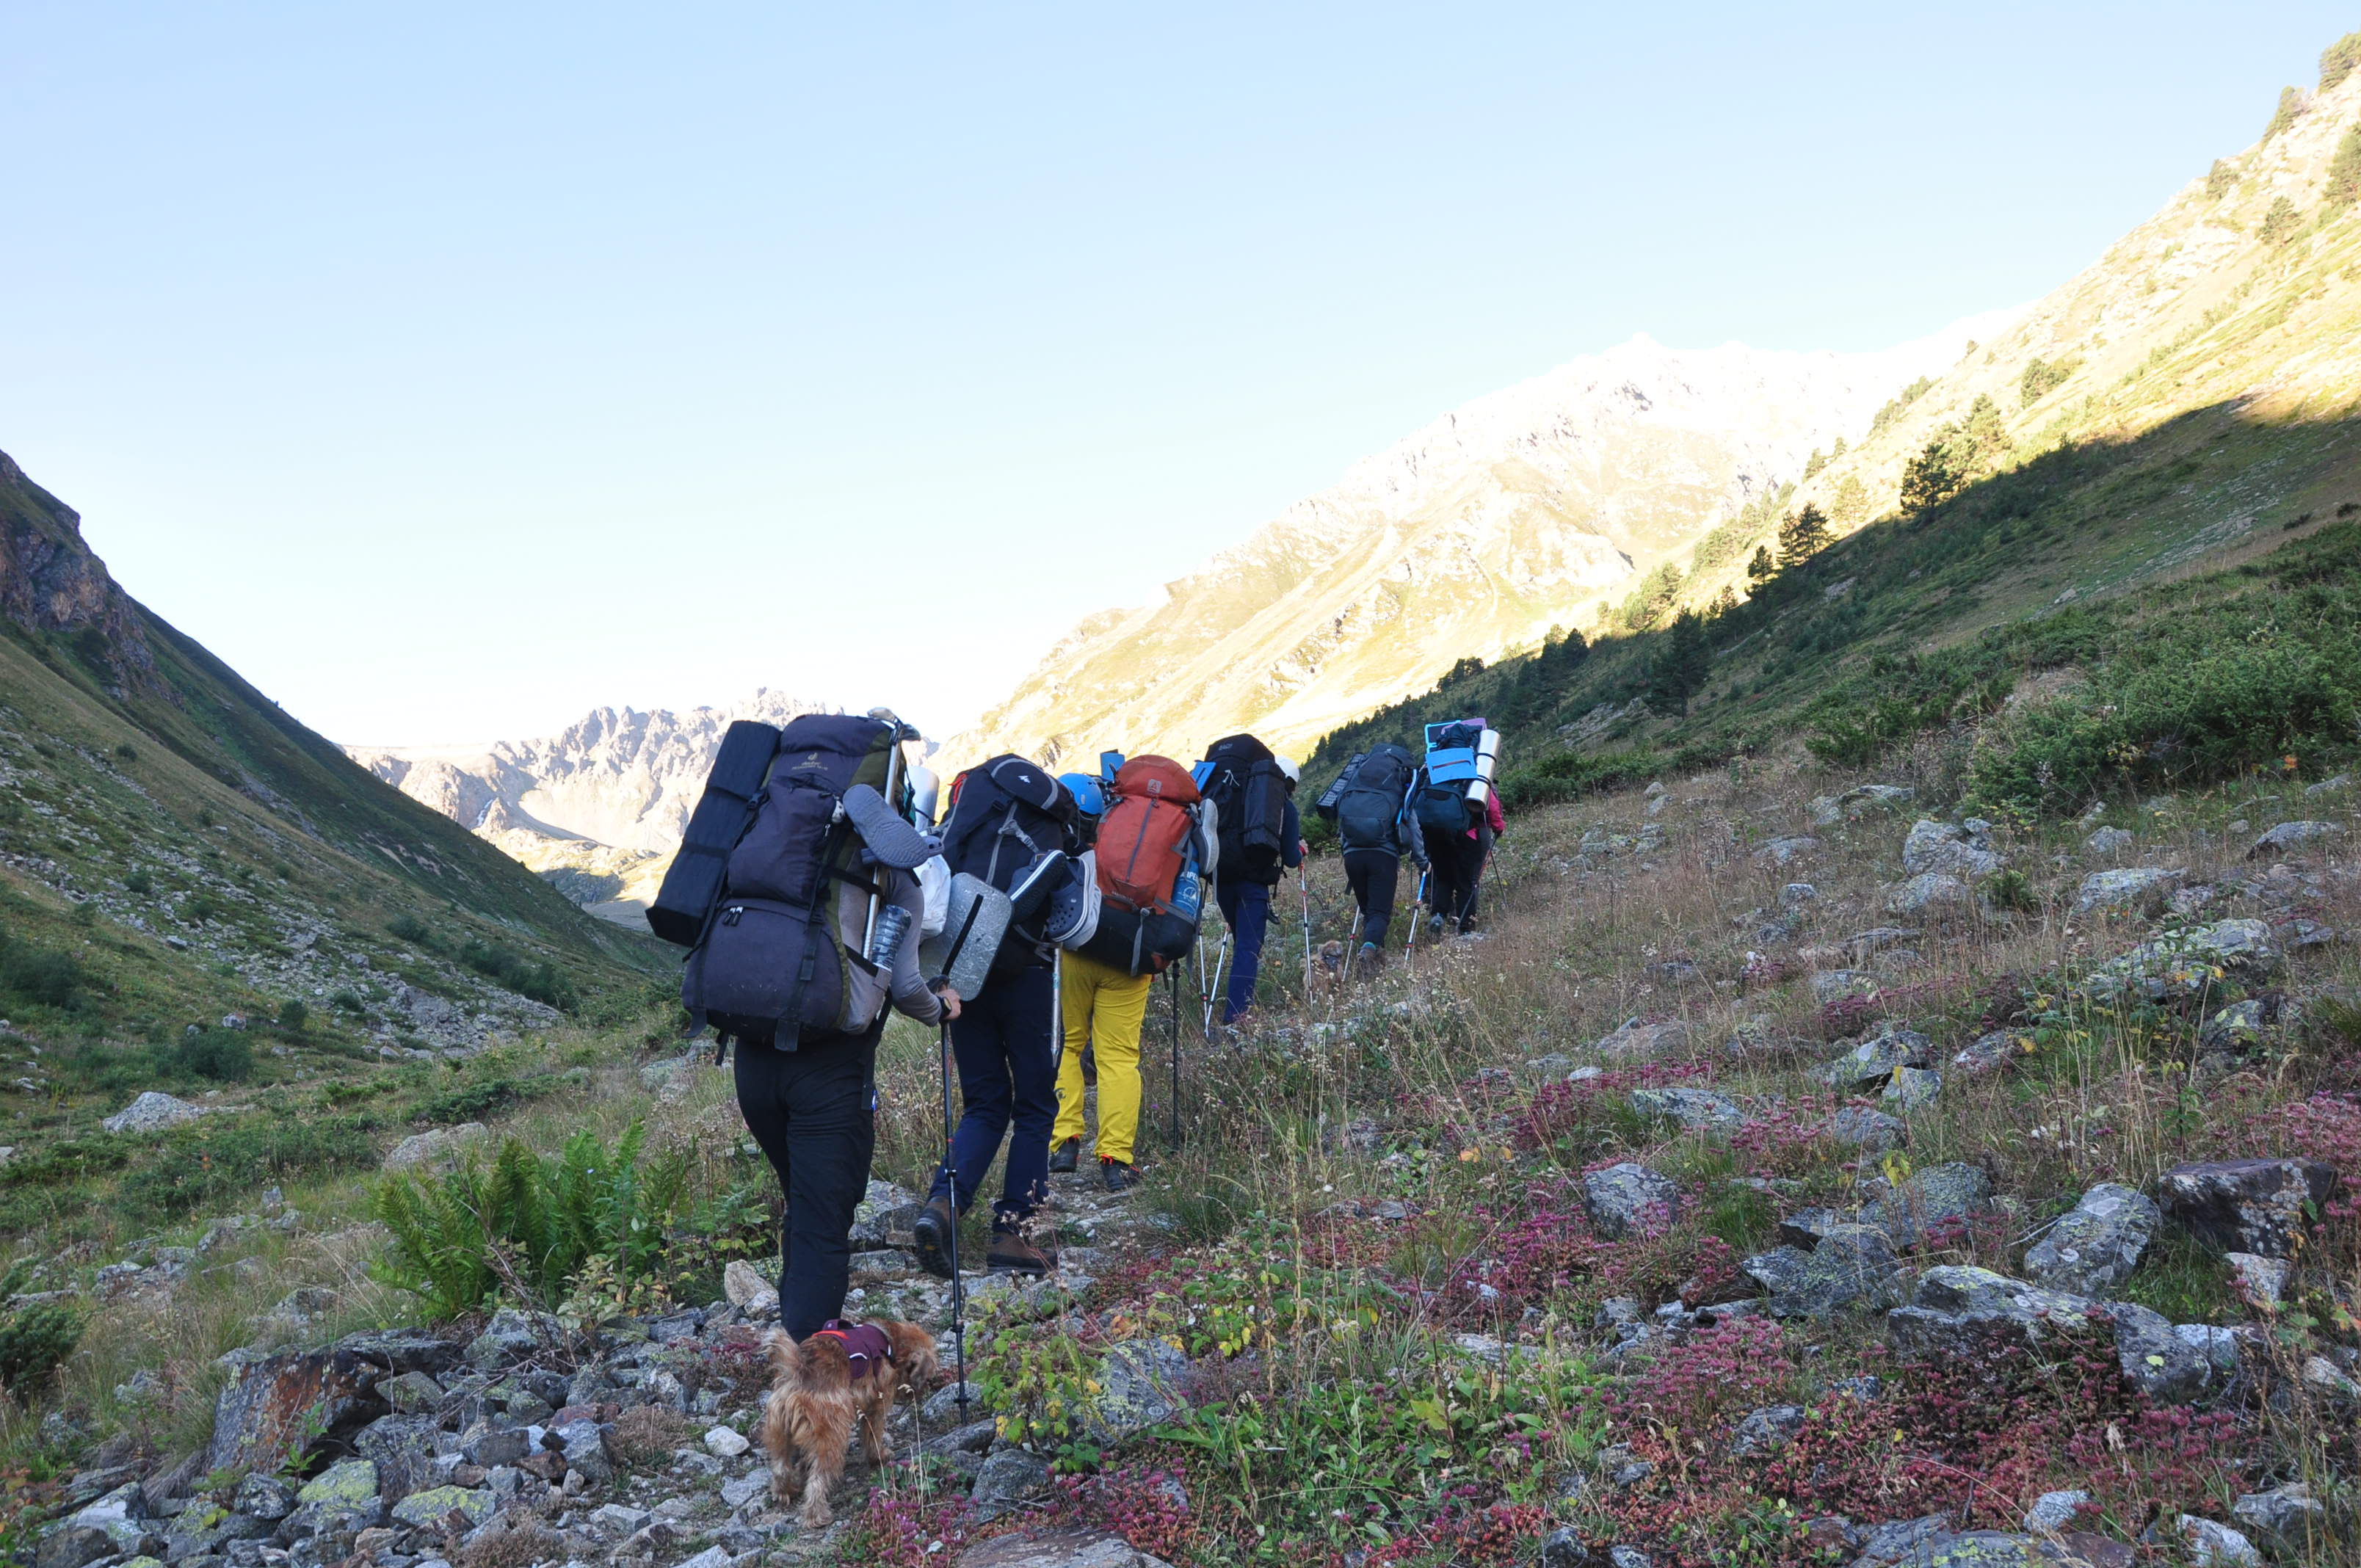
\includegraphics[width=\linewidth]{../pics/DSC_0621}
\end{frame}	


\begin{frame}
	\frametitle{Подъём по древней морене}
	\framesubtitle{День 2, 19 августа}
	\centering
	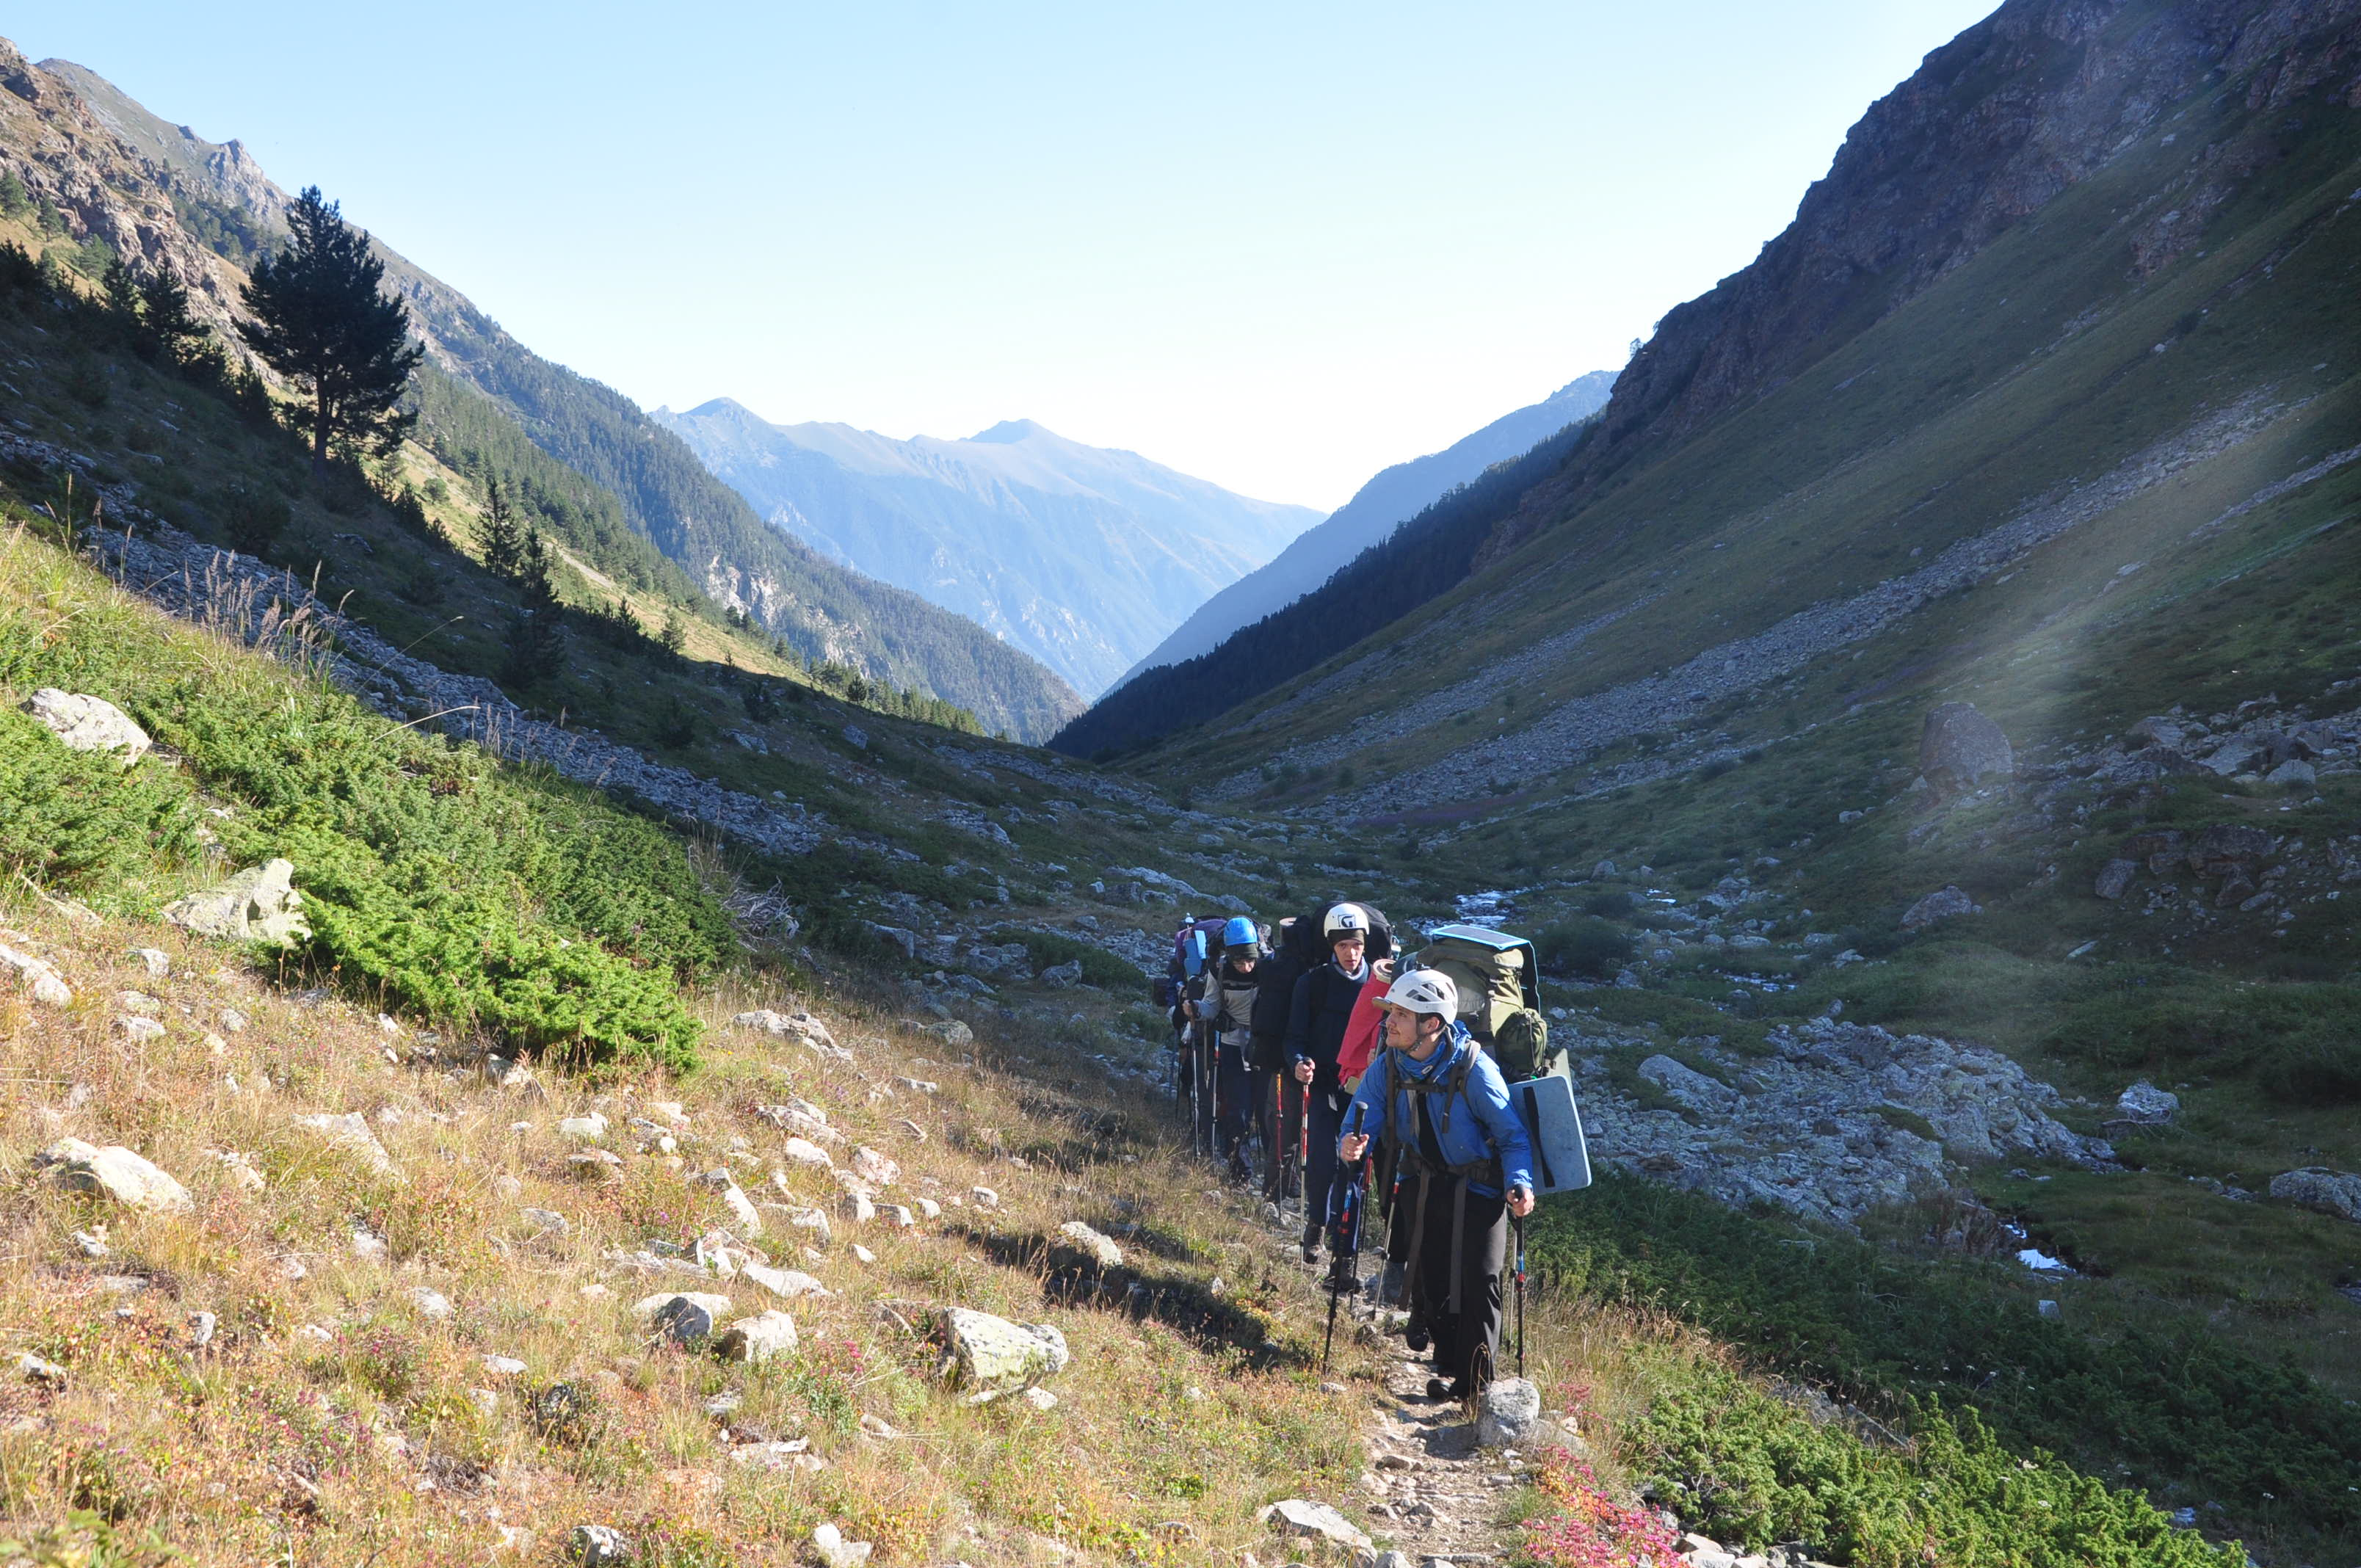
\includegraphics[width=\linewidth]{../pics/DSC_0666}
	\end{frame}

\begin{frame}
%	\frametitle{}
	\framesubtitle{День 2, 19 августа}
	\centering
	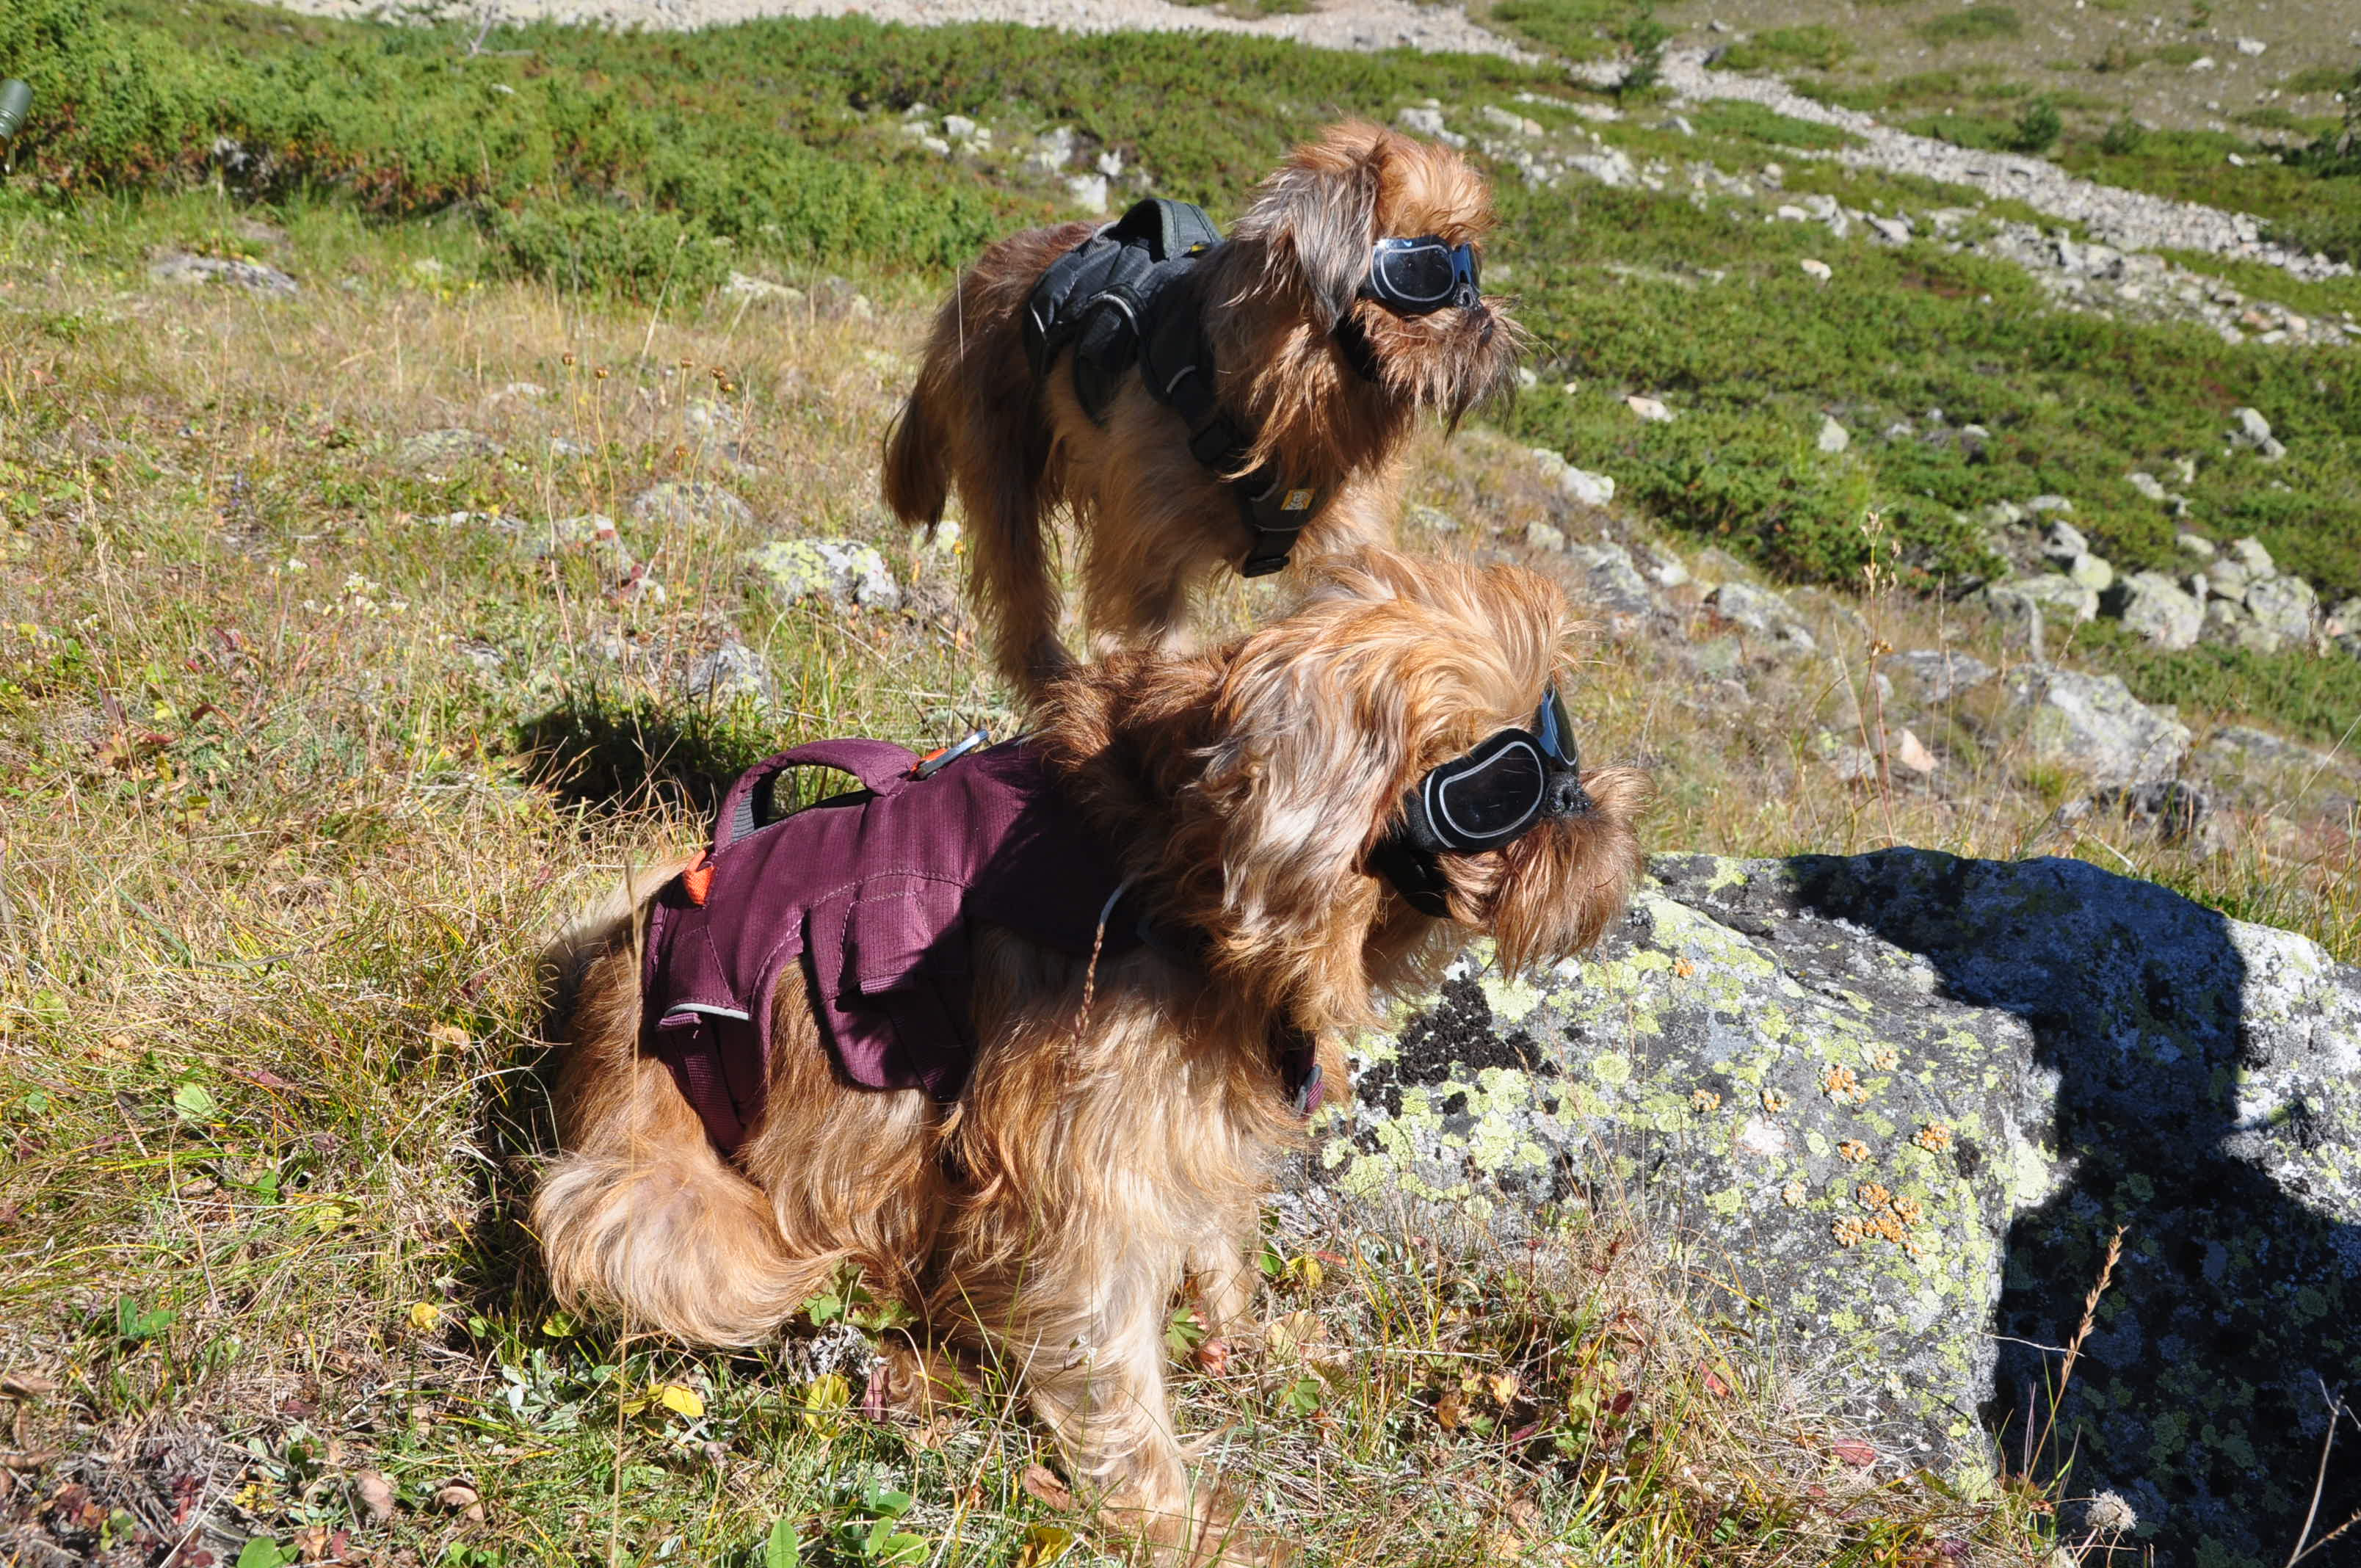
\includegraphics[width=\linewidth]{../pics/DSC_0683}
	\end{frame}

\begin{frame}
%	\frametitle{Дорога до озёр и далее на перевал}
	\framesubtitle{День 2, 19 августа}
	\centering
	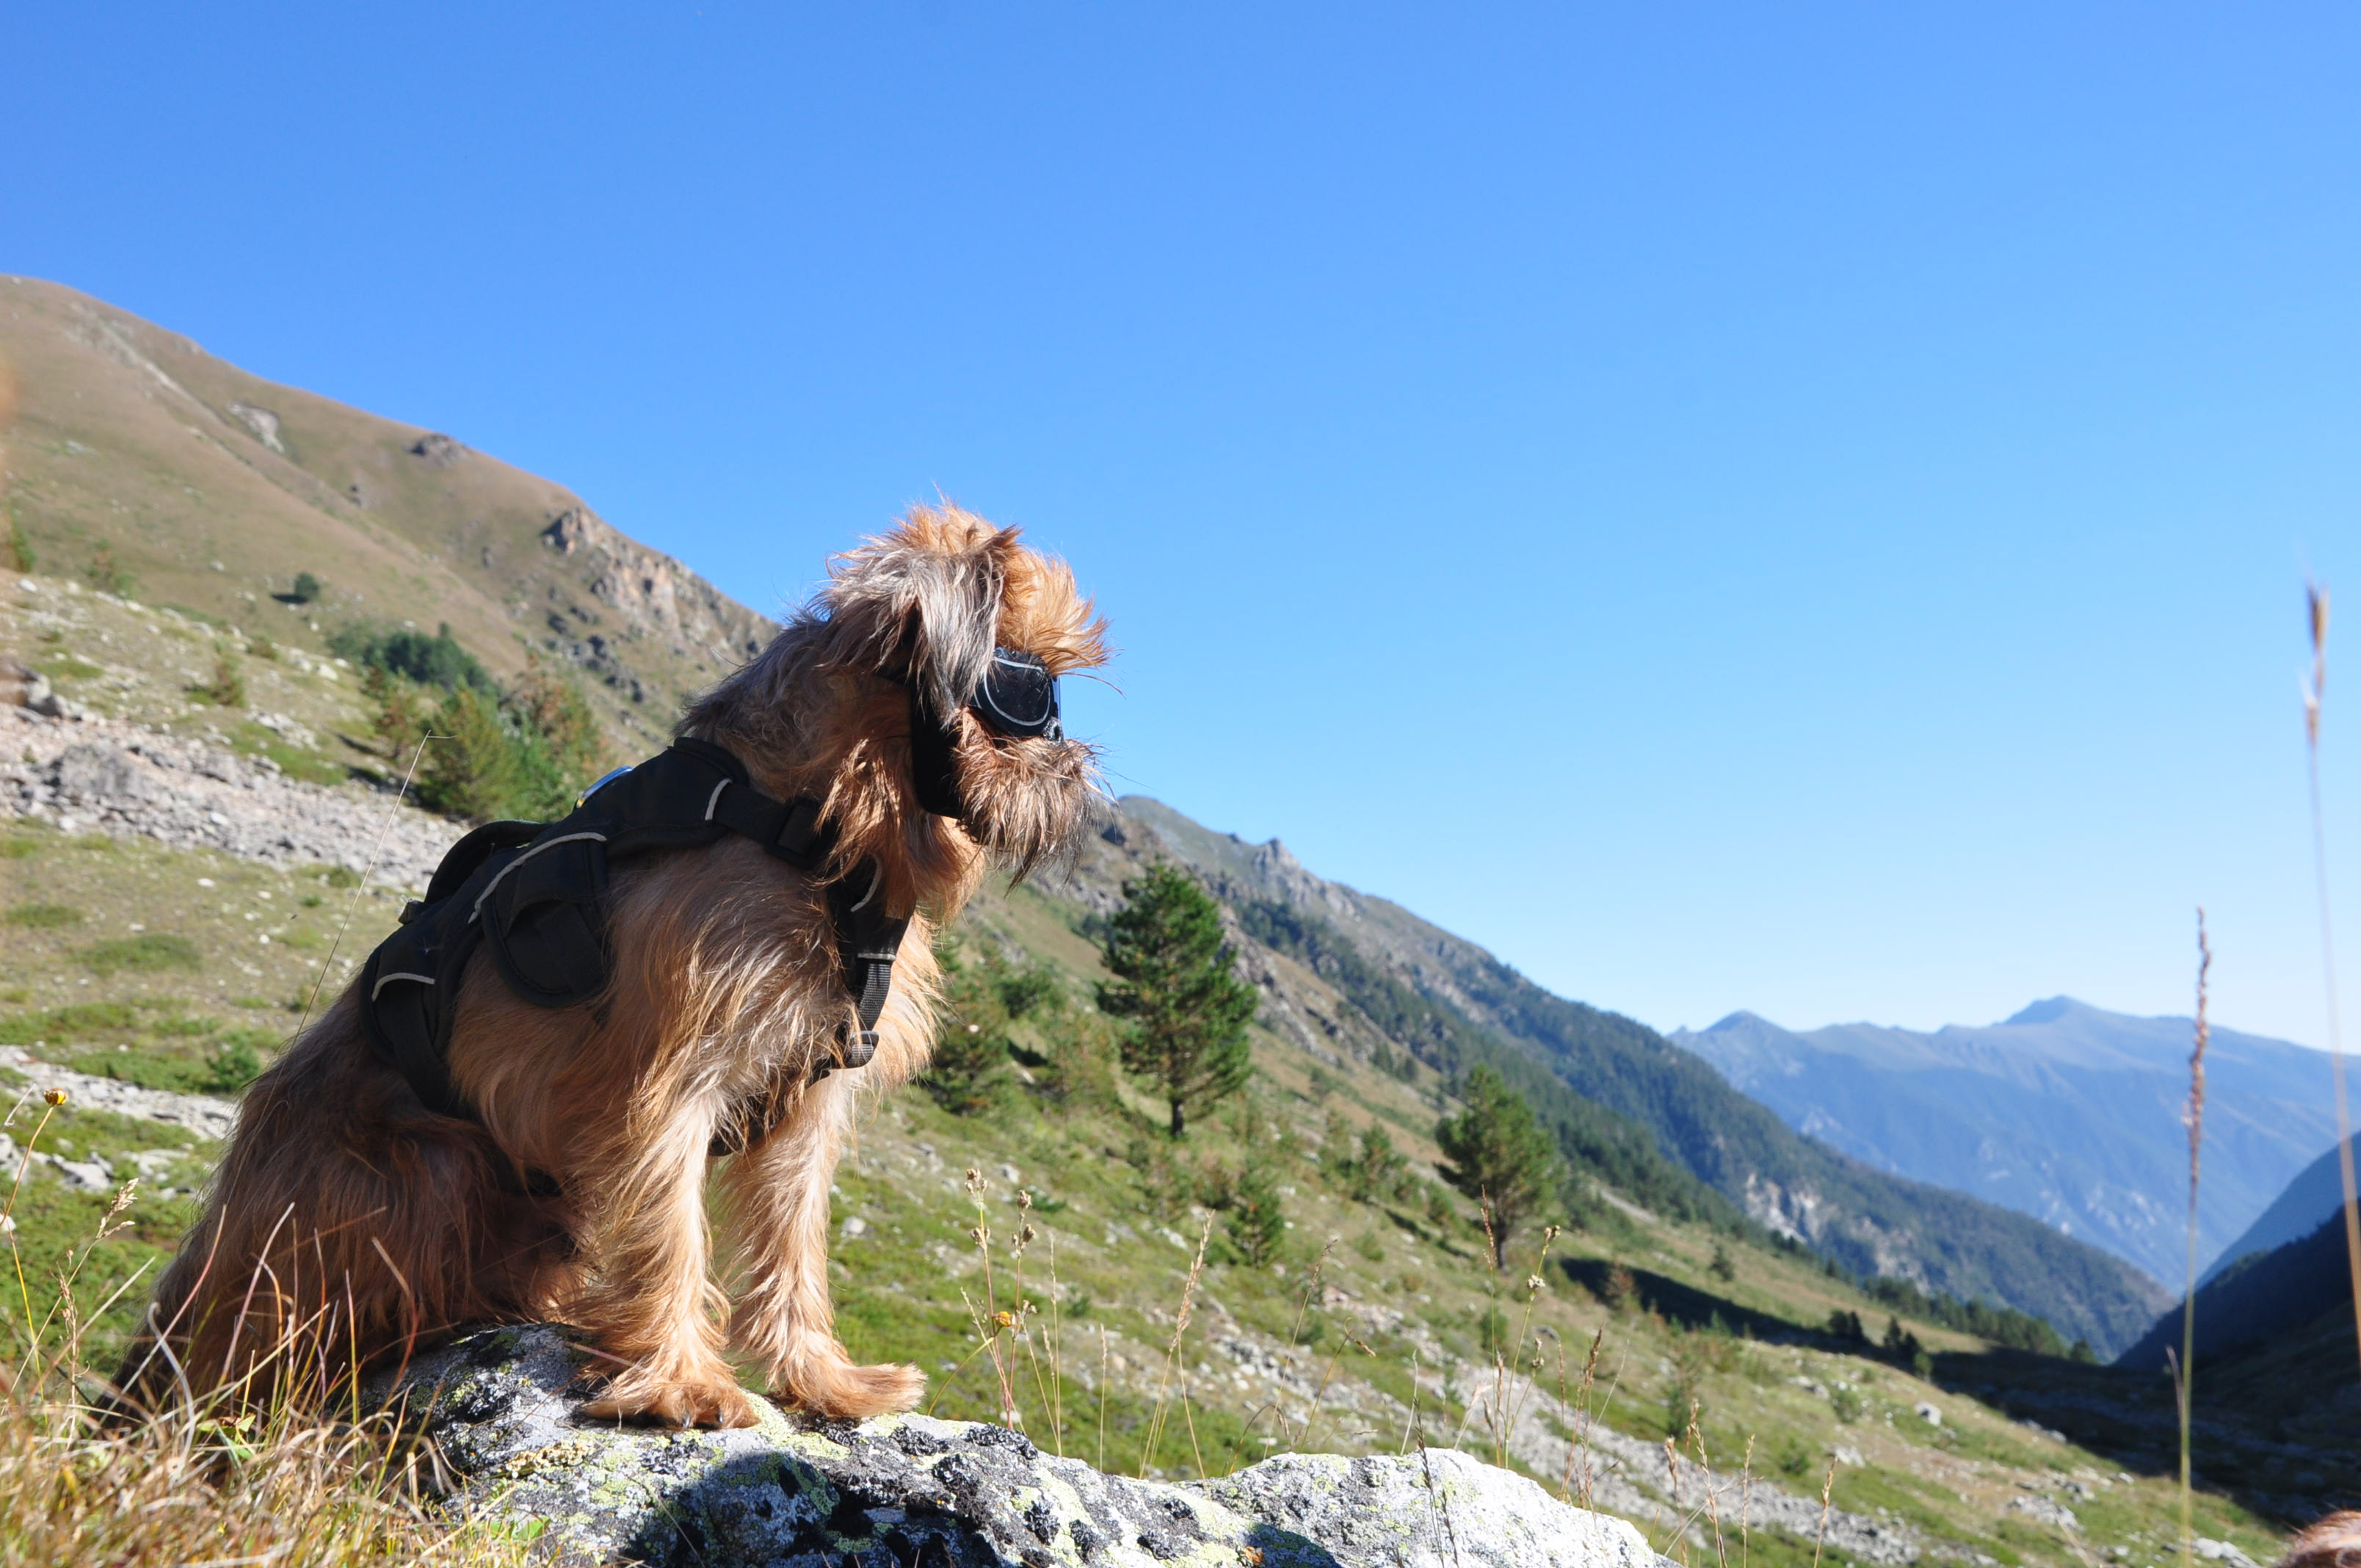
\includegraphics[width=\linewidth]{../pics/DSC_0687}
	\end{frame}

\begin{frame}
	\frametitle{Верховья д.р. Кичкинакол Уллукёльский, вид на север}
	\framesubtitle{День 2, 19 августа}
	\centering
	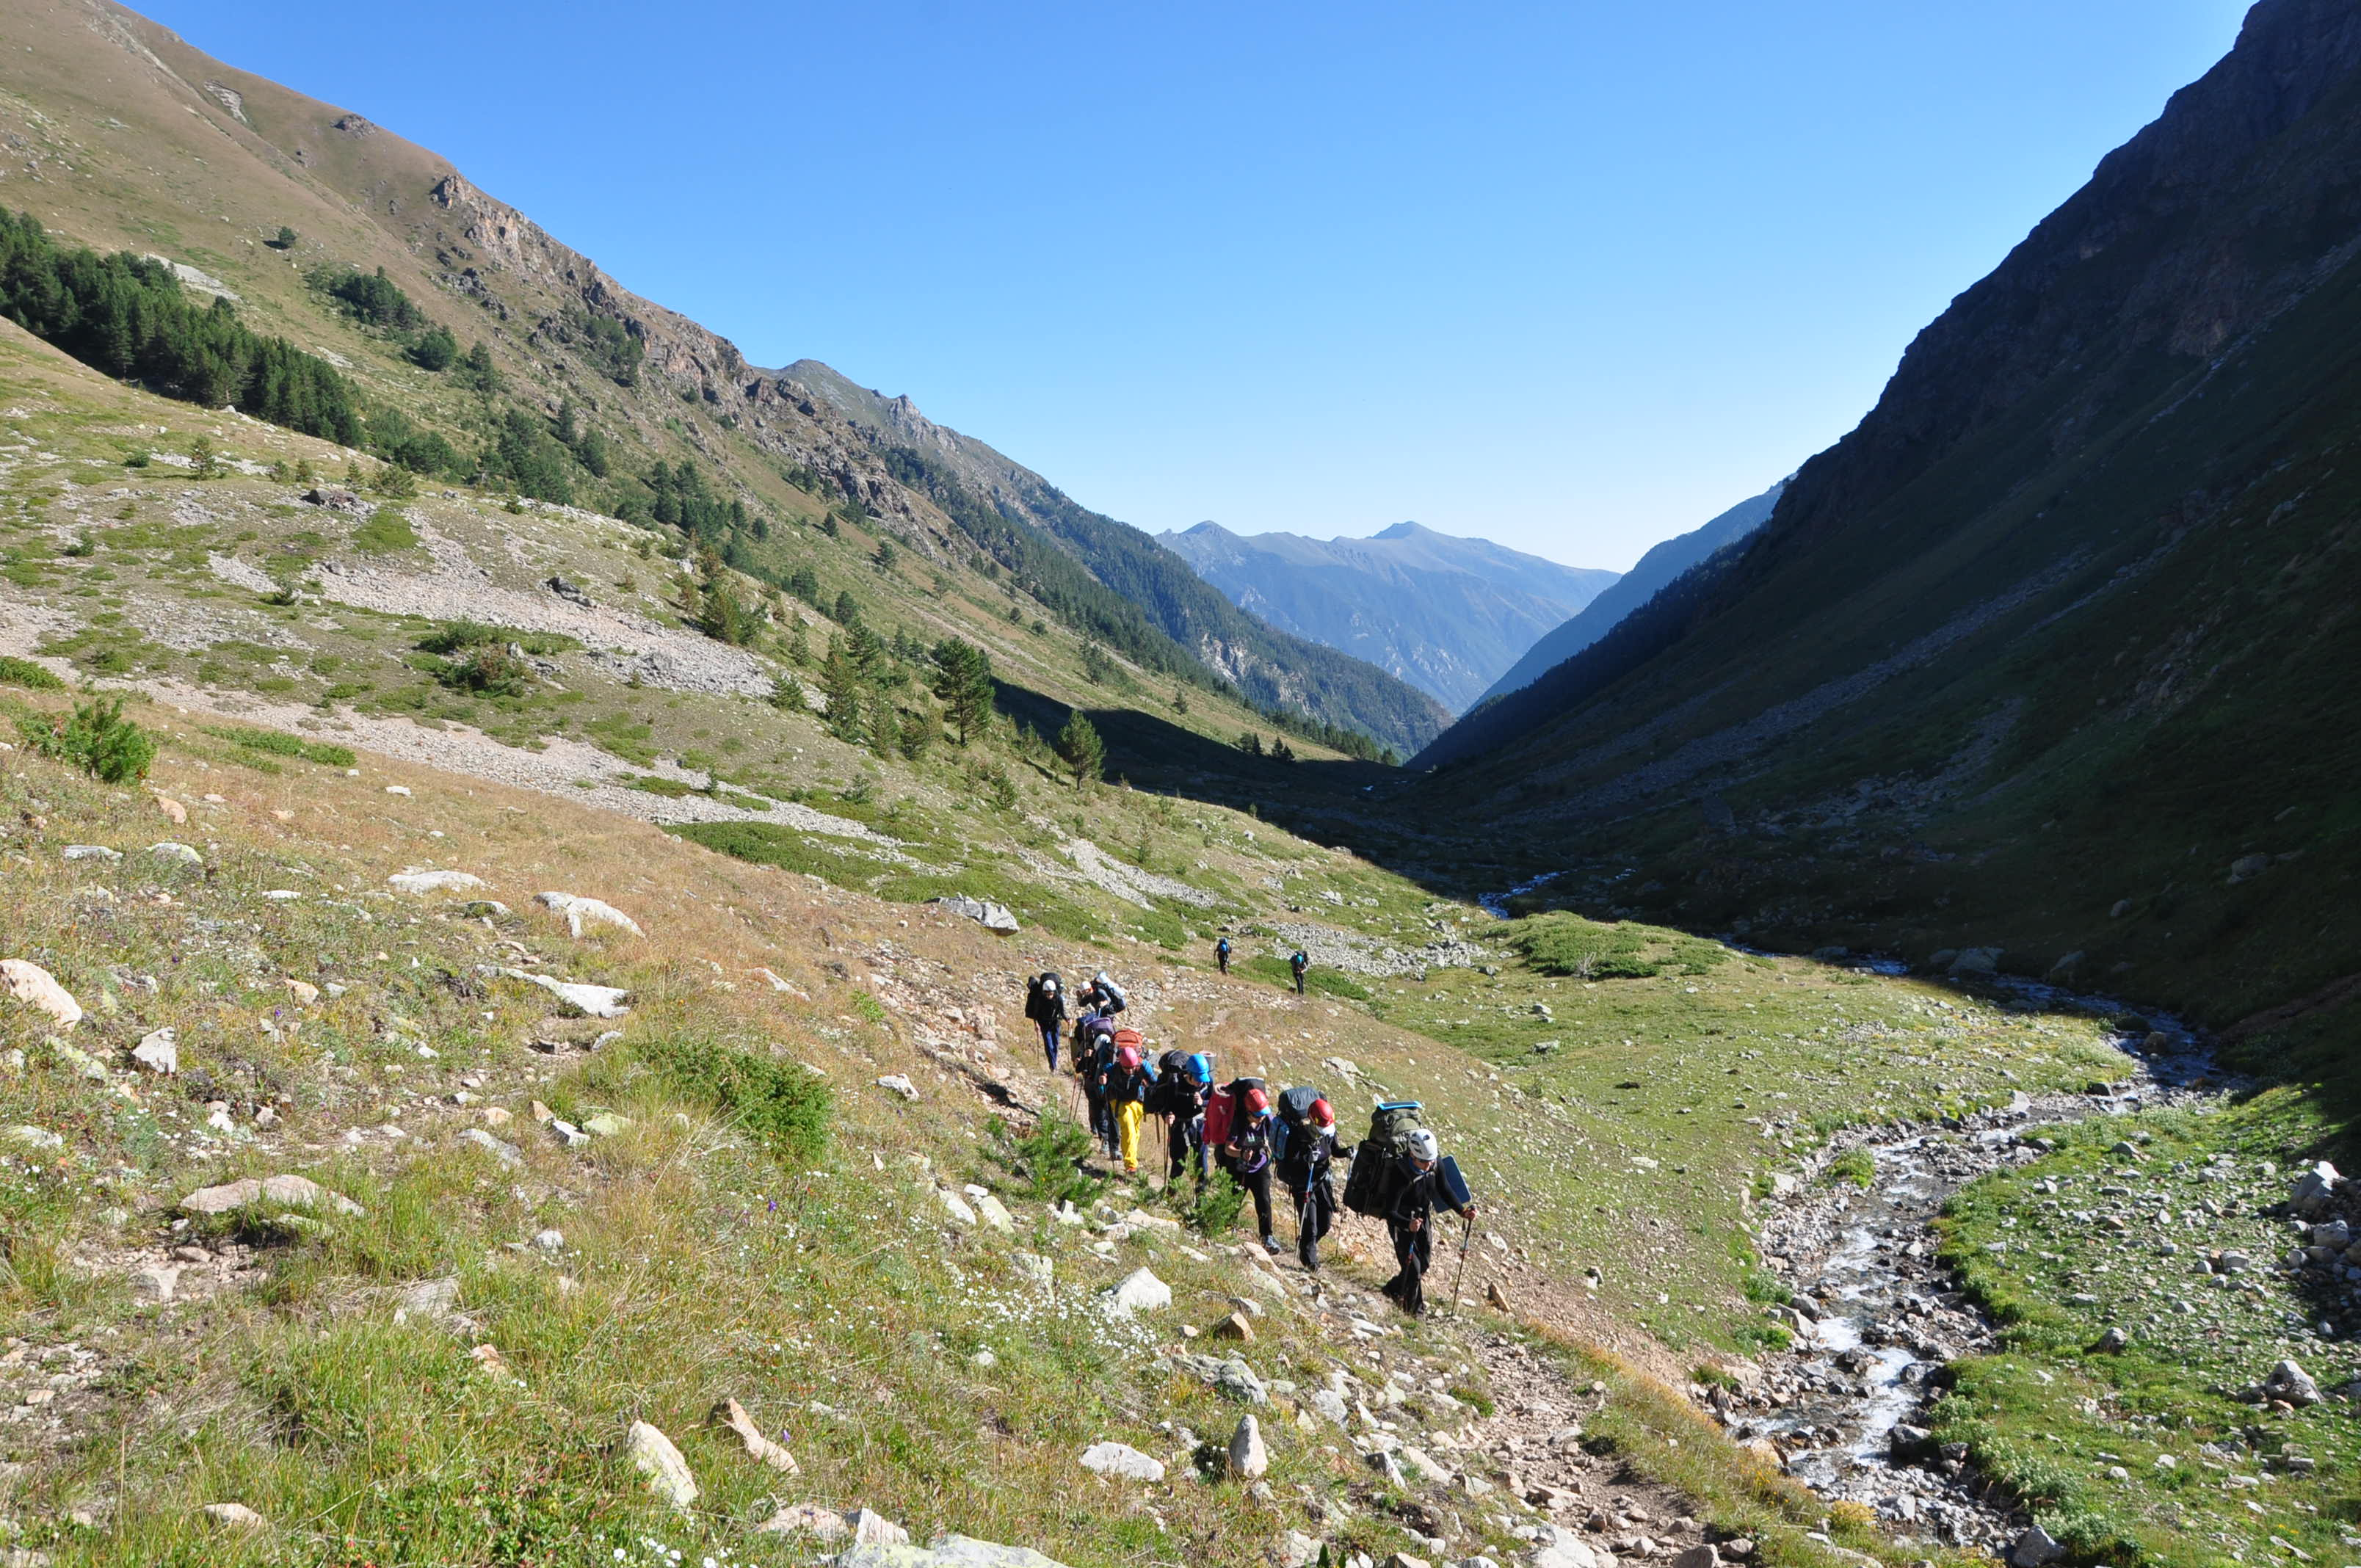
\includegraphics[width=\linewidth]{../pics/DSC_0696}
	\end{frame}

\begin{frame}
	\frametitle{Шафран}
	\framesubtitle{День 2, 19 августа}
	\centering
	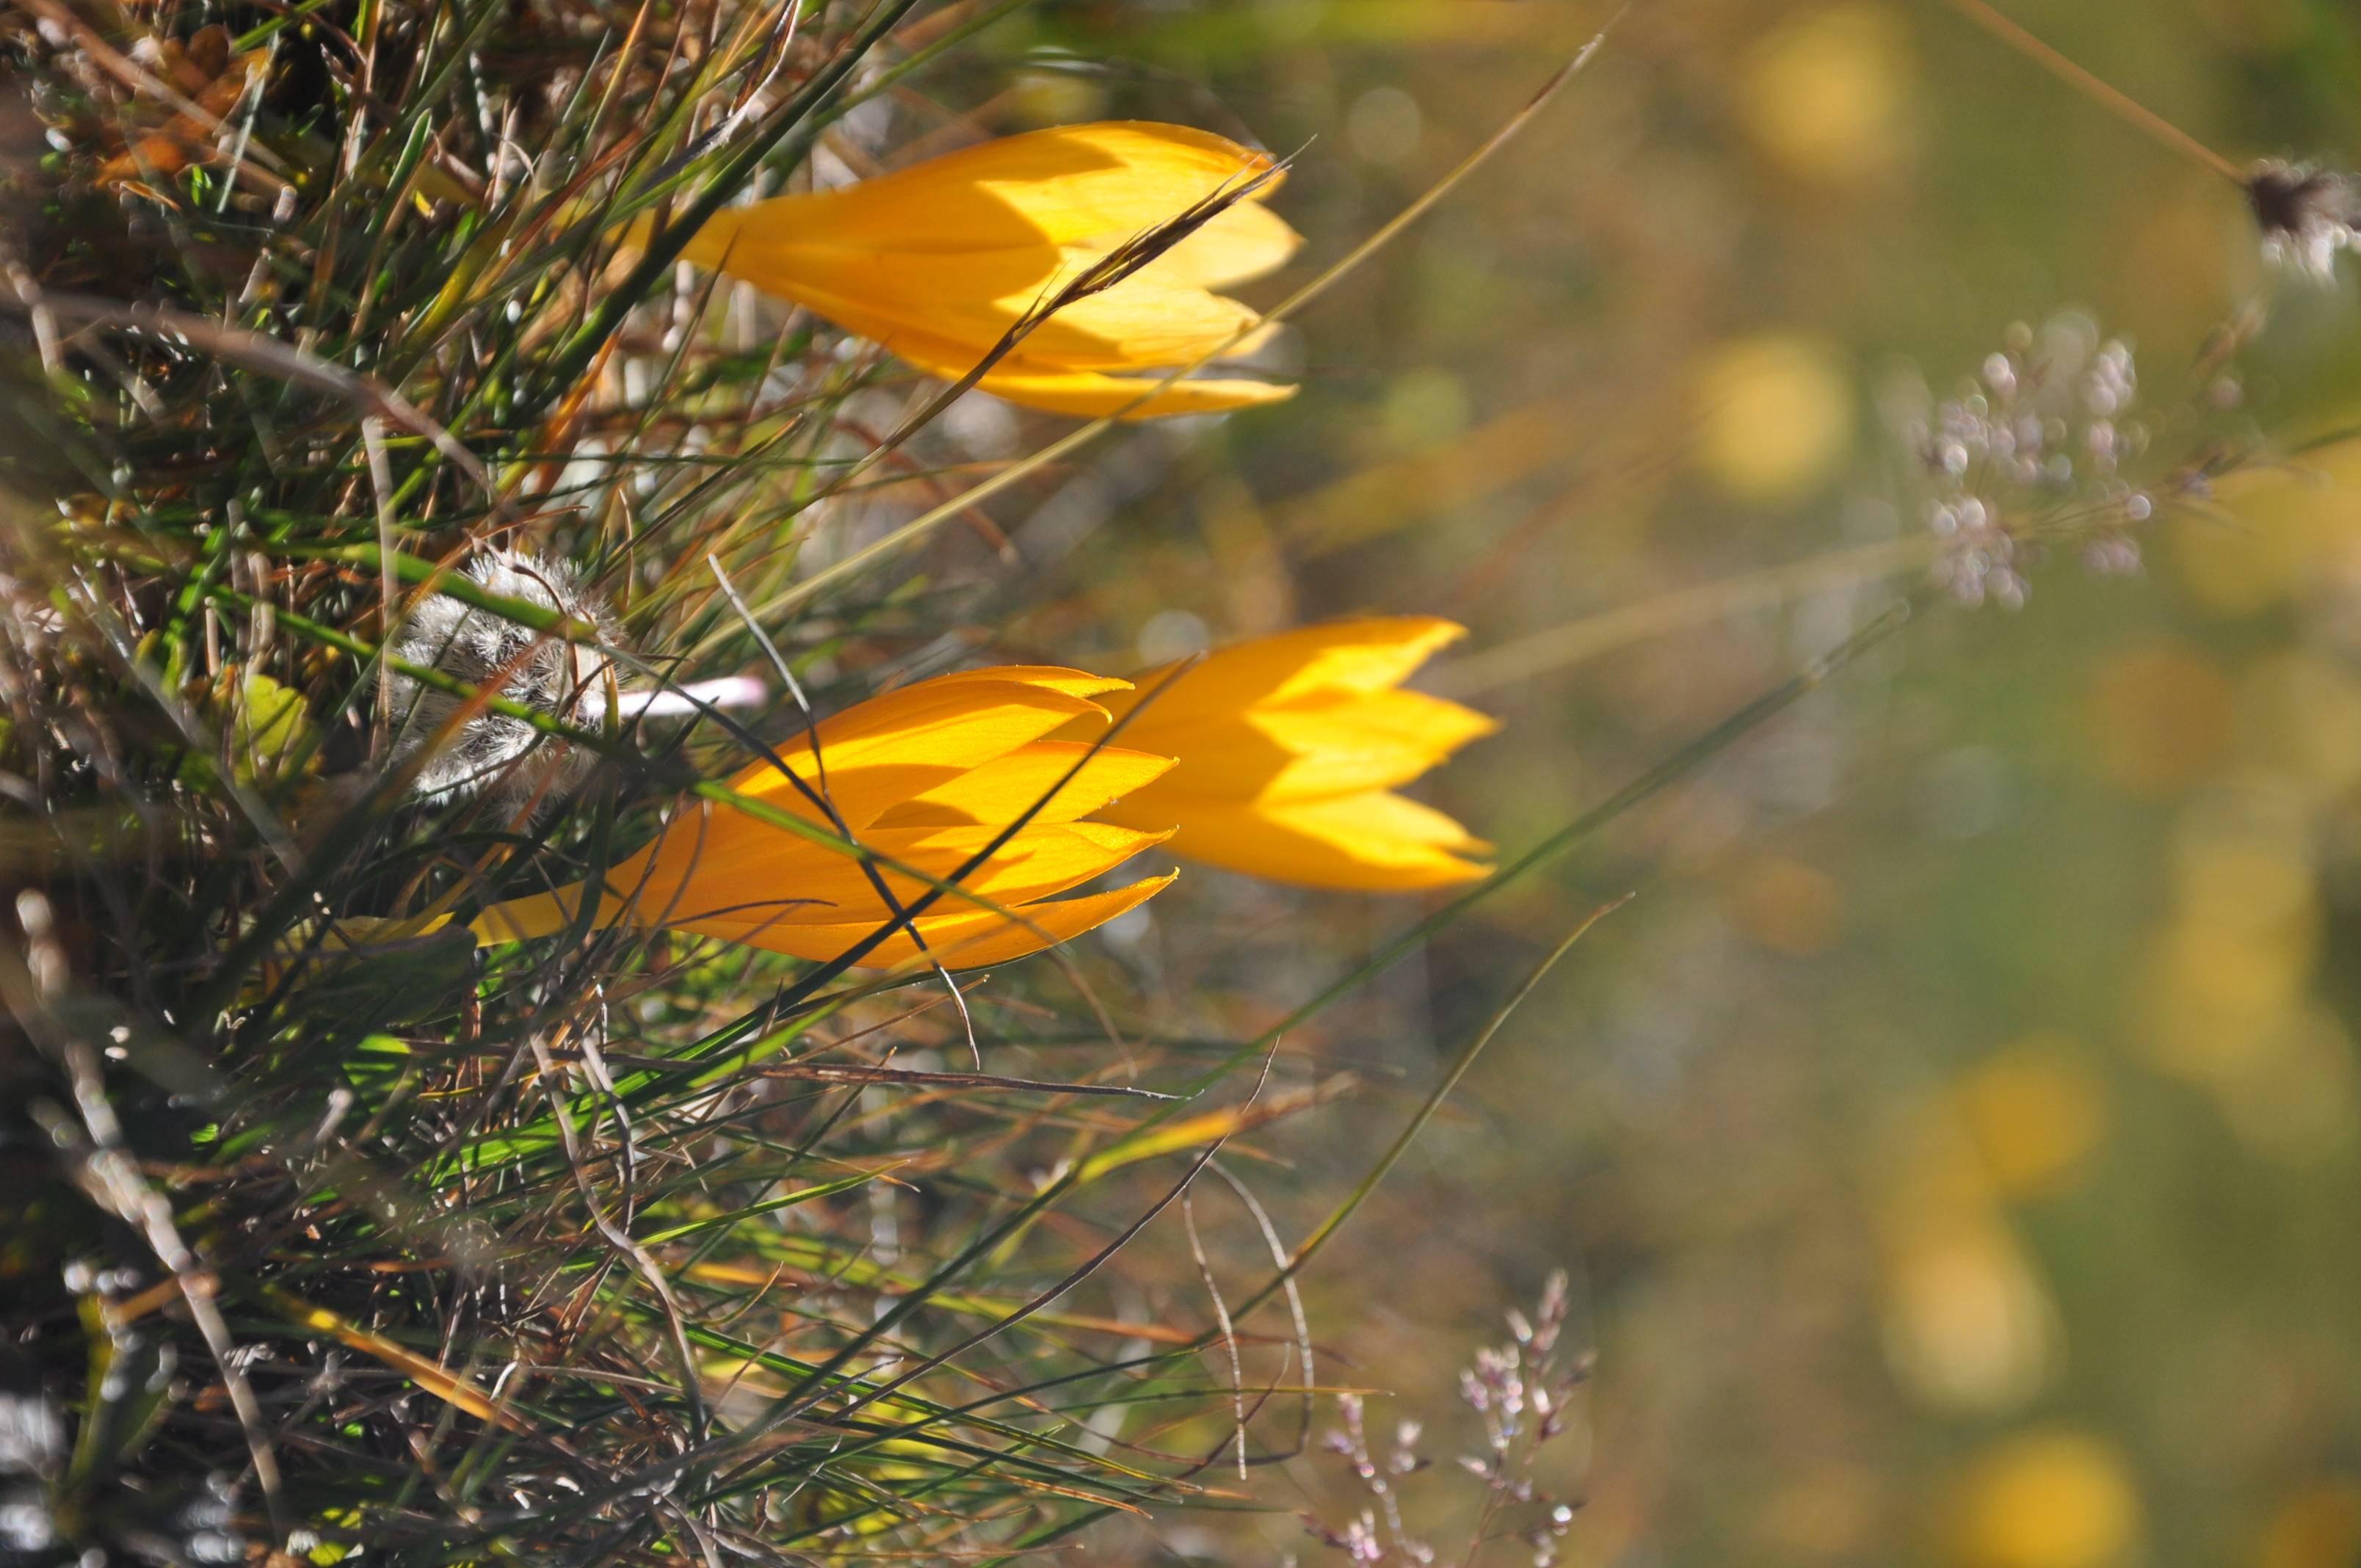
\includegraphics[width=\linewidth]{../pics/DSC_0725}
	\end{frame}

\begin{frame}
	\frametitle{Какие-то цветочки}
	\framesubtitle{День 2, 19 августа}
	\centering
	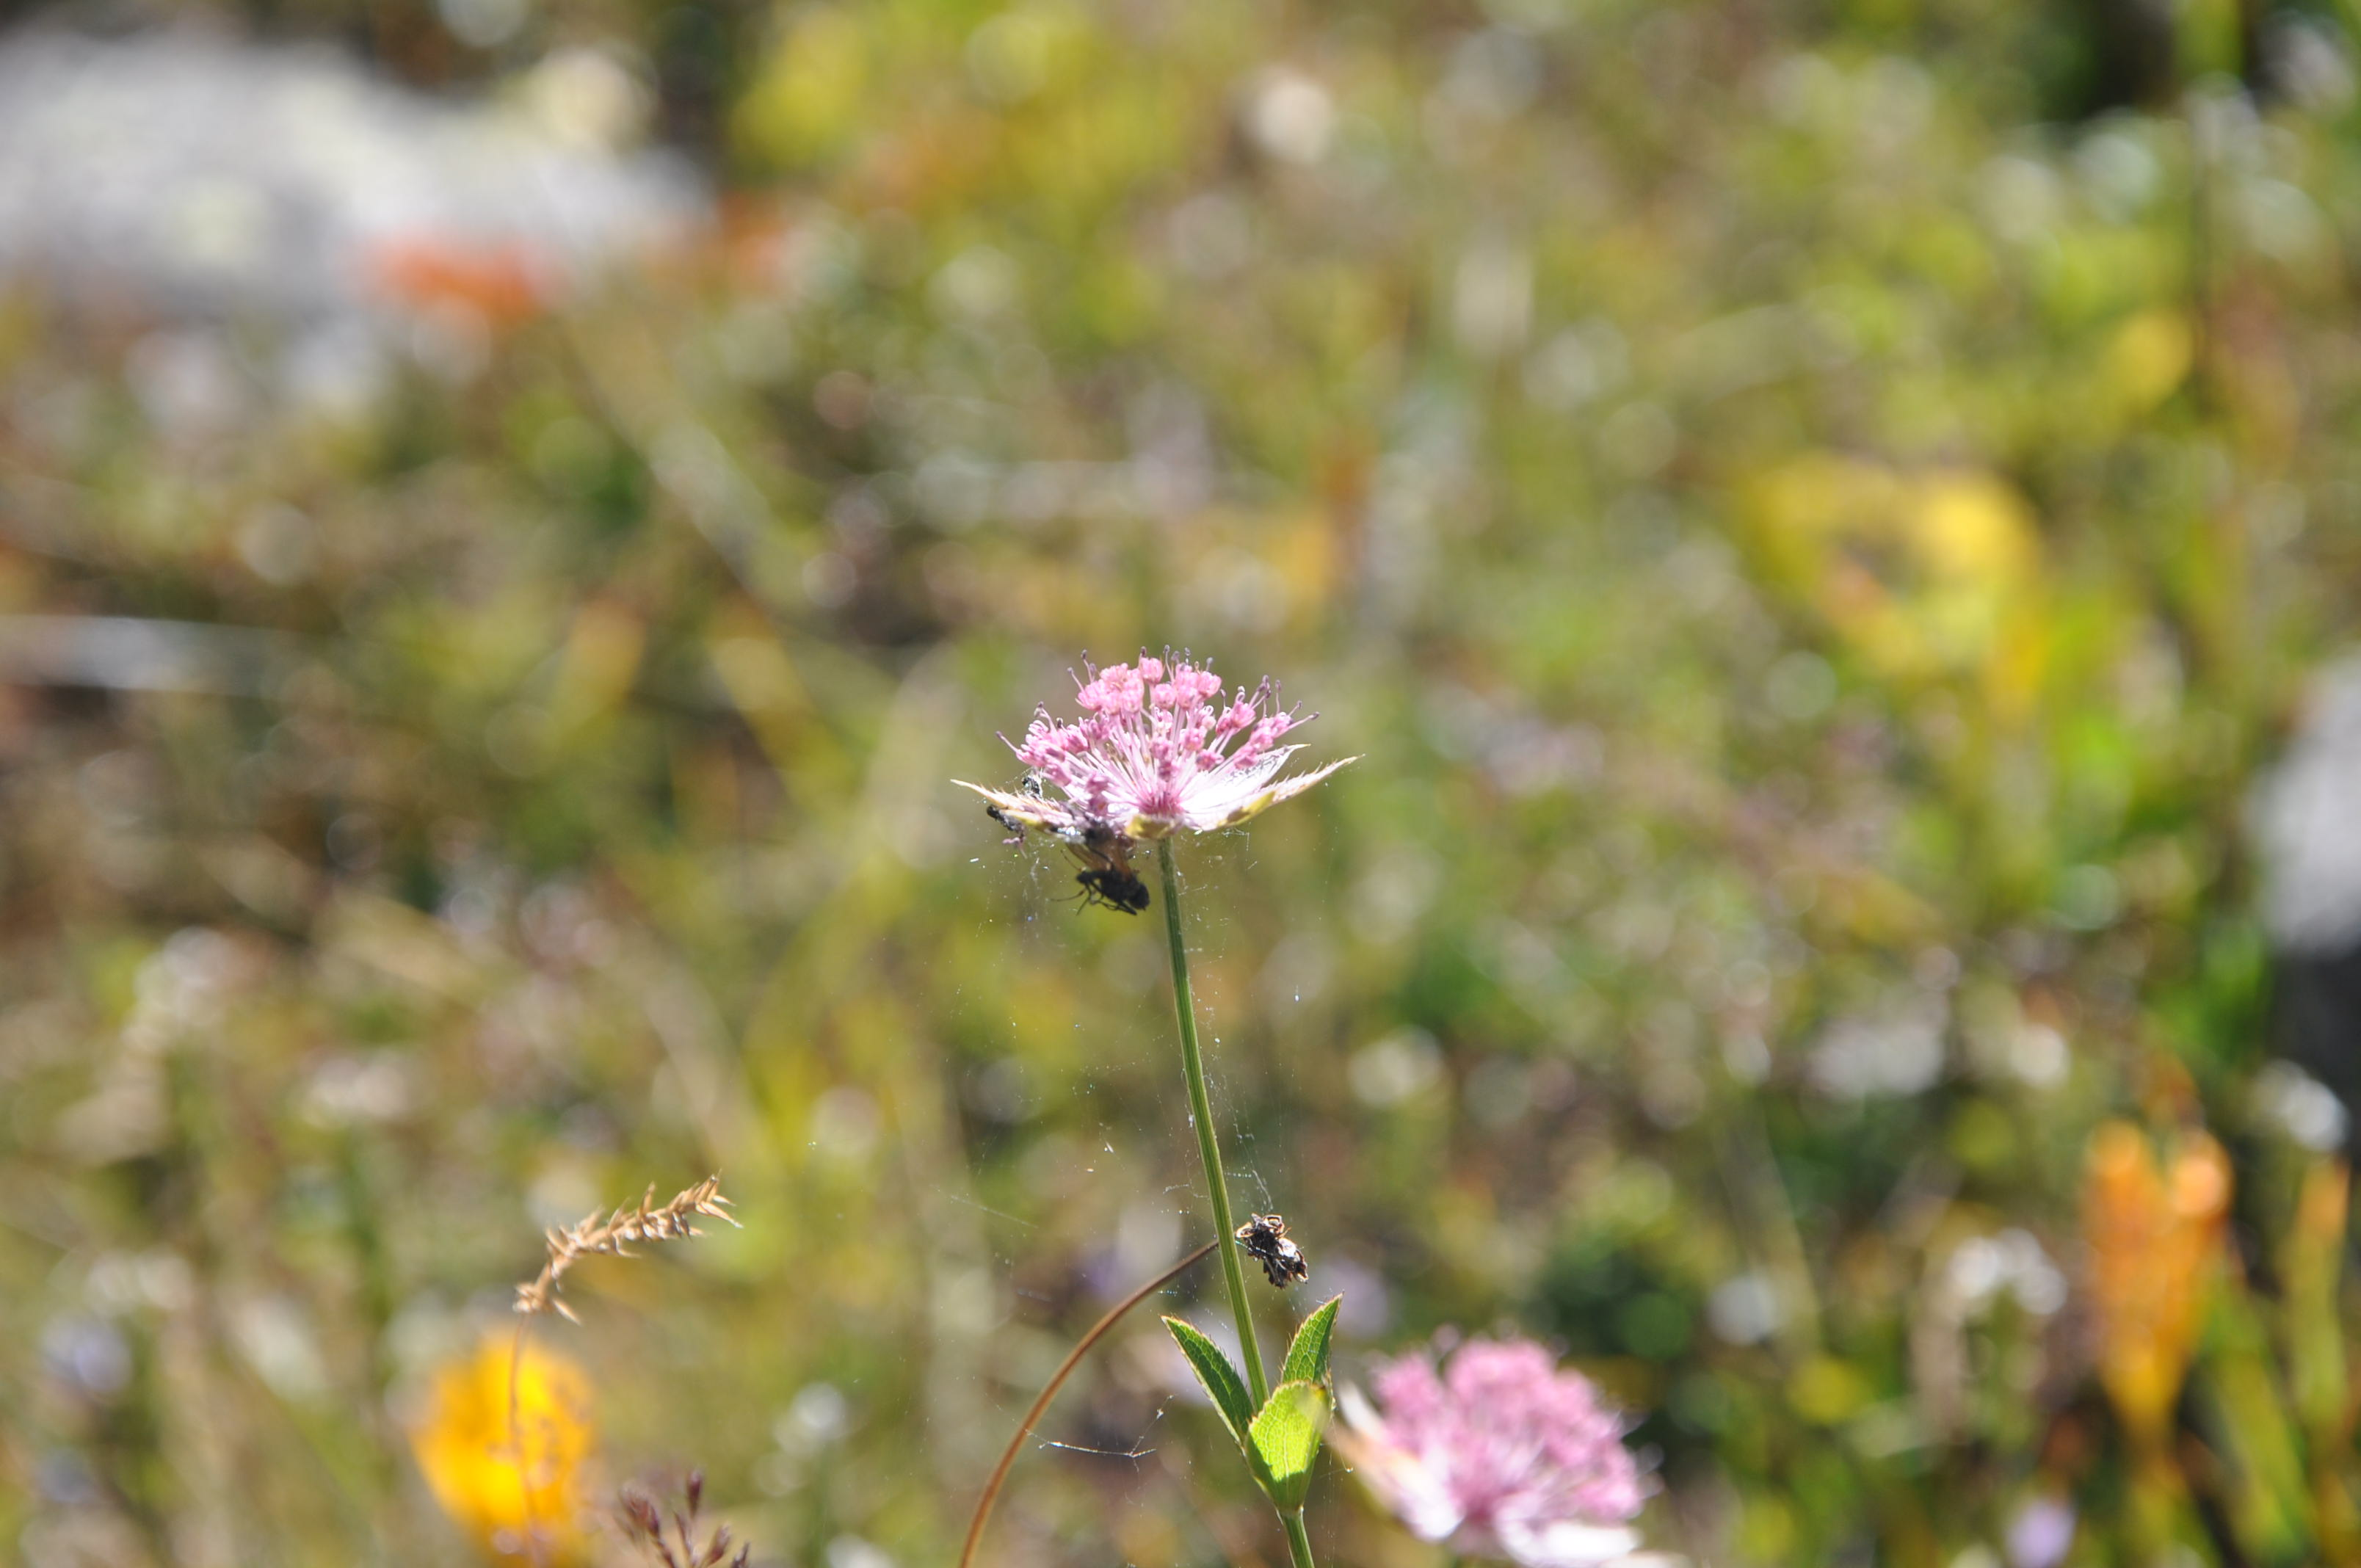
\includegraphics[width=\linewidth]{../pics/DSC_0732}
\end{frame}

\begin{frame}
	\frametitle{На озере Уллу-Кёль <<Большое озеро>>}
	\framesubtitle{День 2, 19 августа}
	\centering
	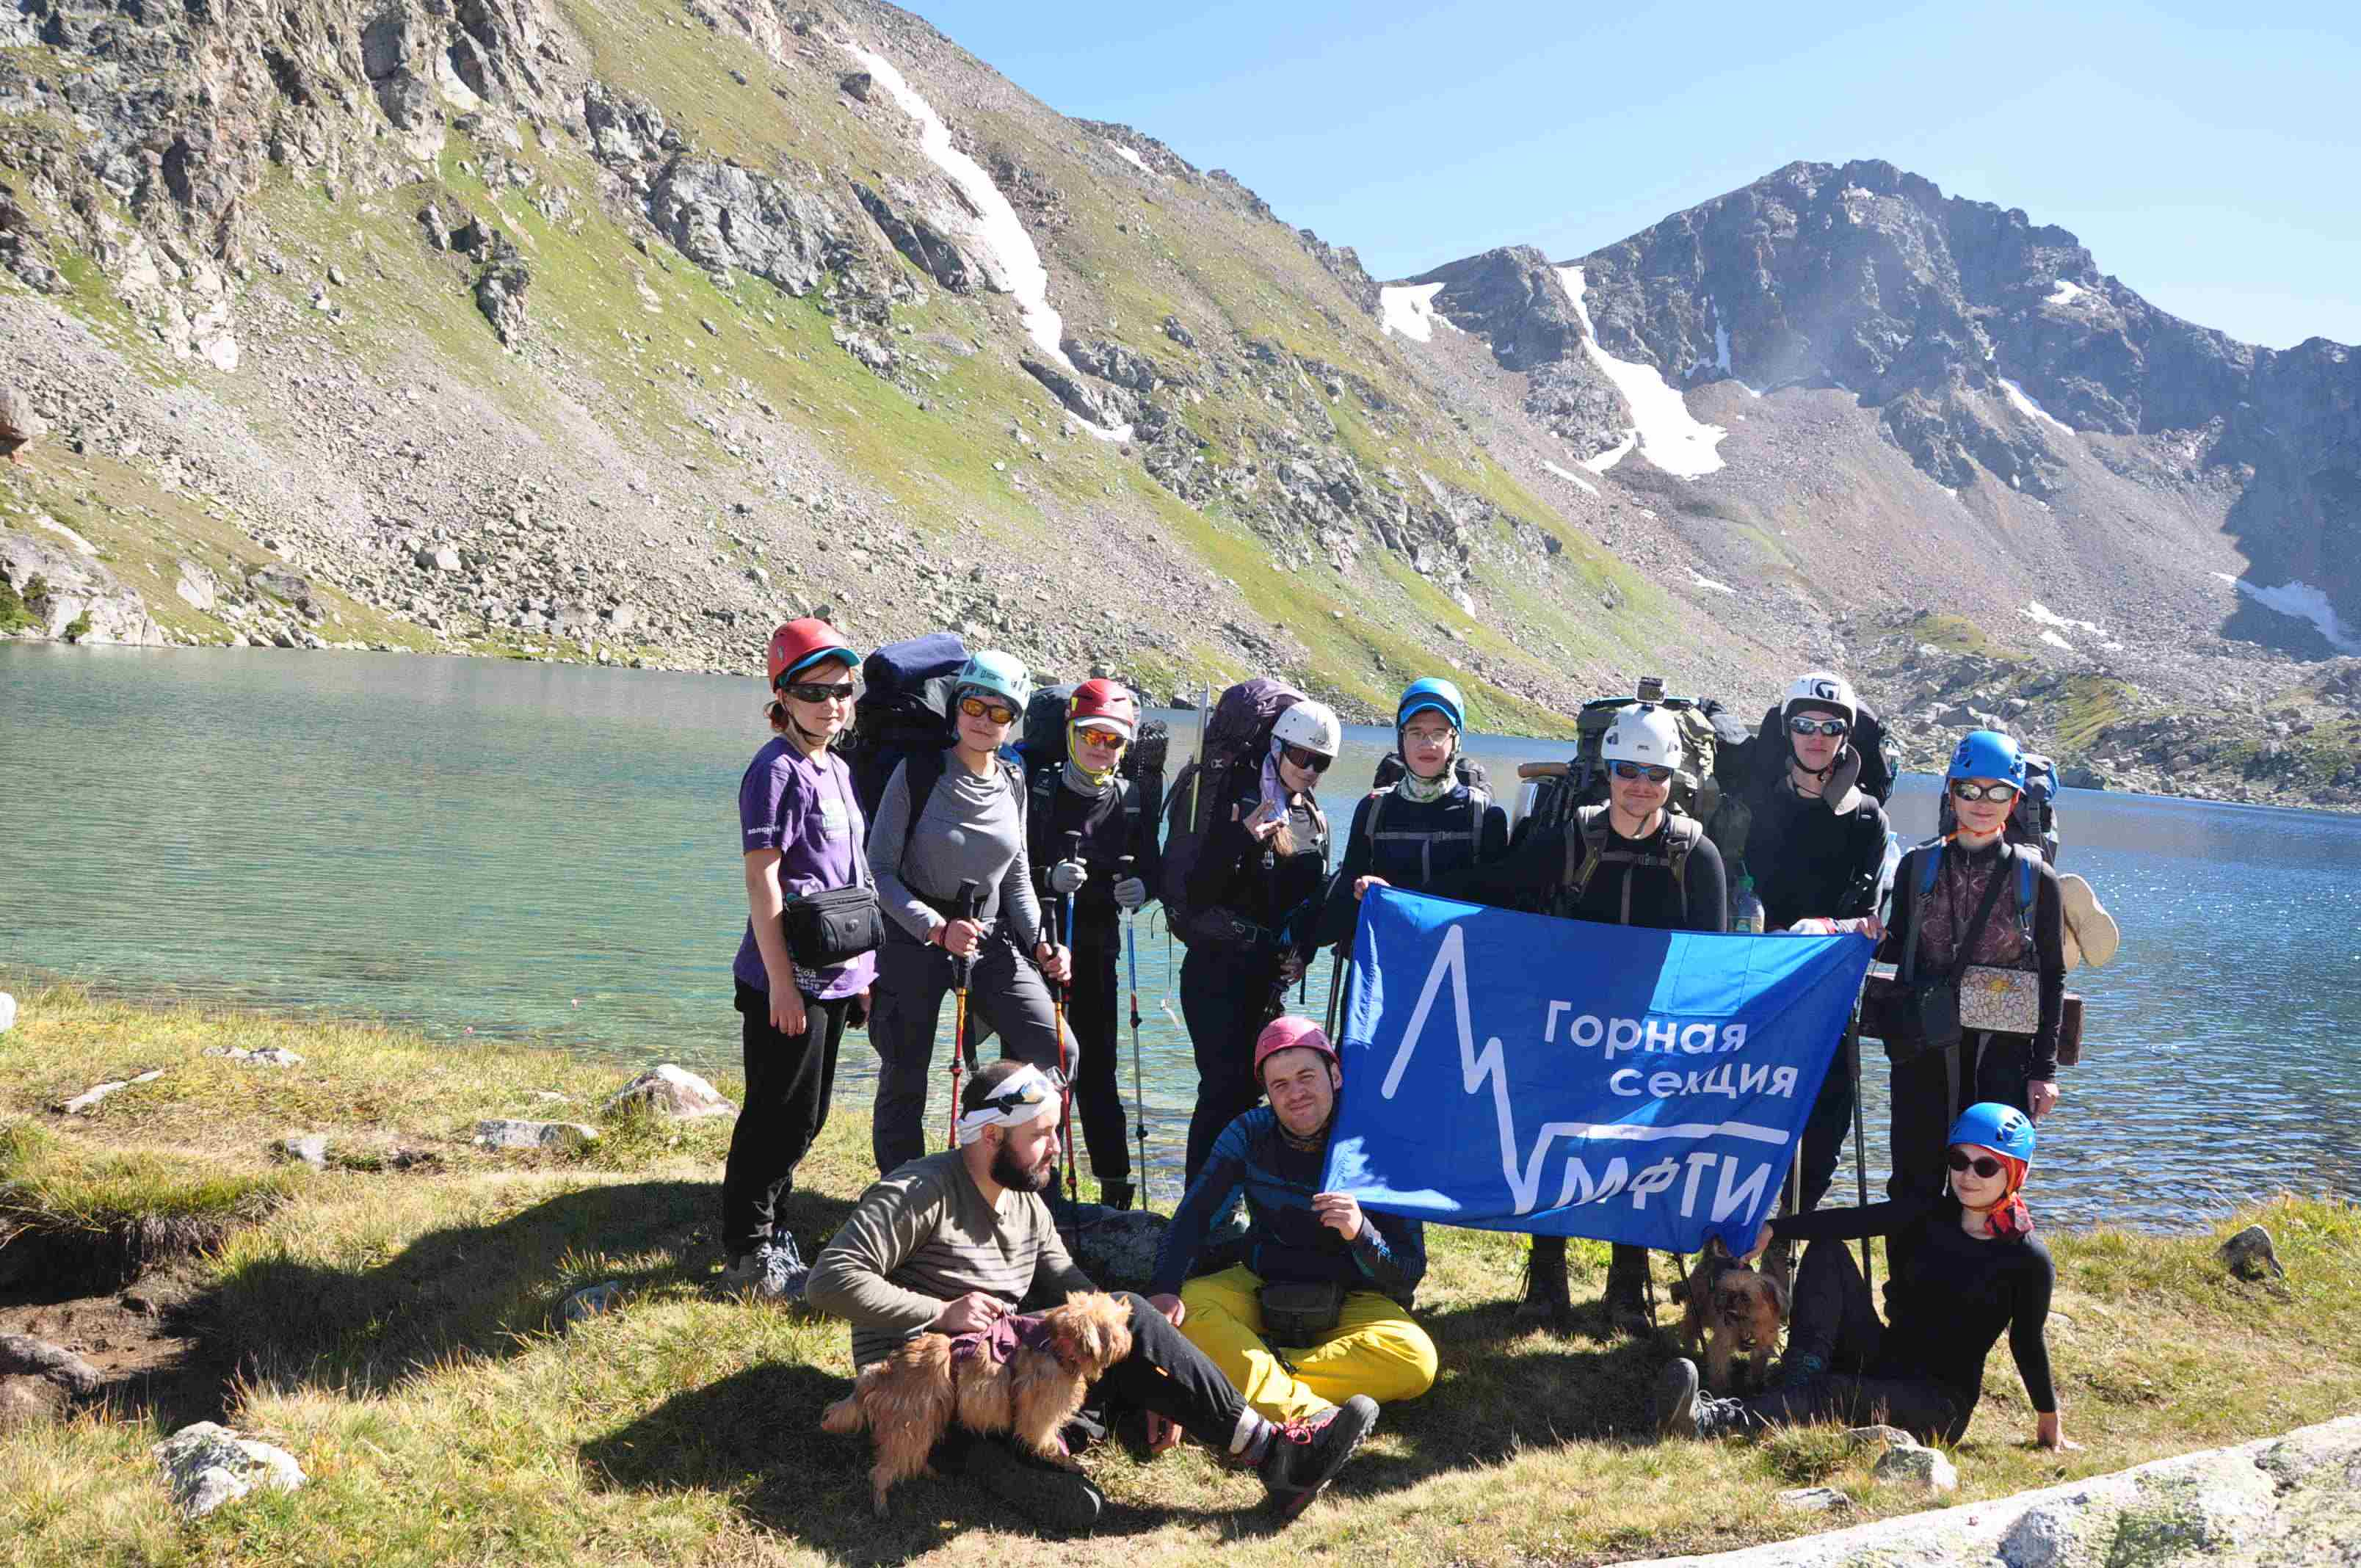
\includegraphics[width=\linewidth]{../pics/DSC_0800}
\end{frame}

\begin{frame}
	\frametitle{Уллу-Кёль, идём к м.н.}
	\framesubtitle{День 2, 19 августа}
	\centering
	\rotatebox{-90}{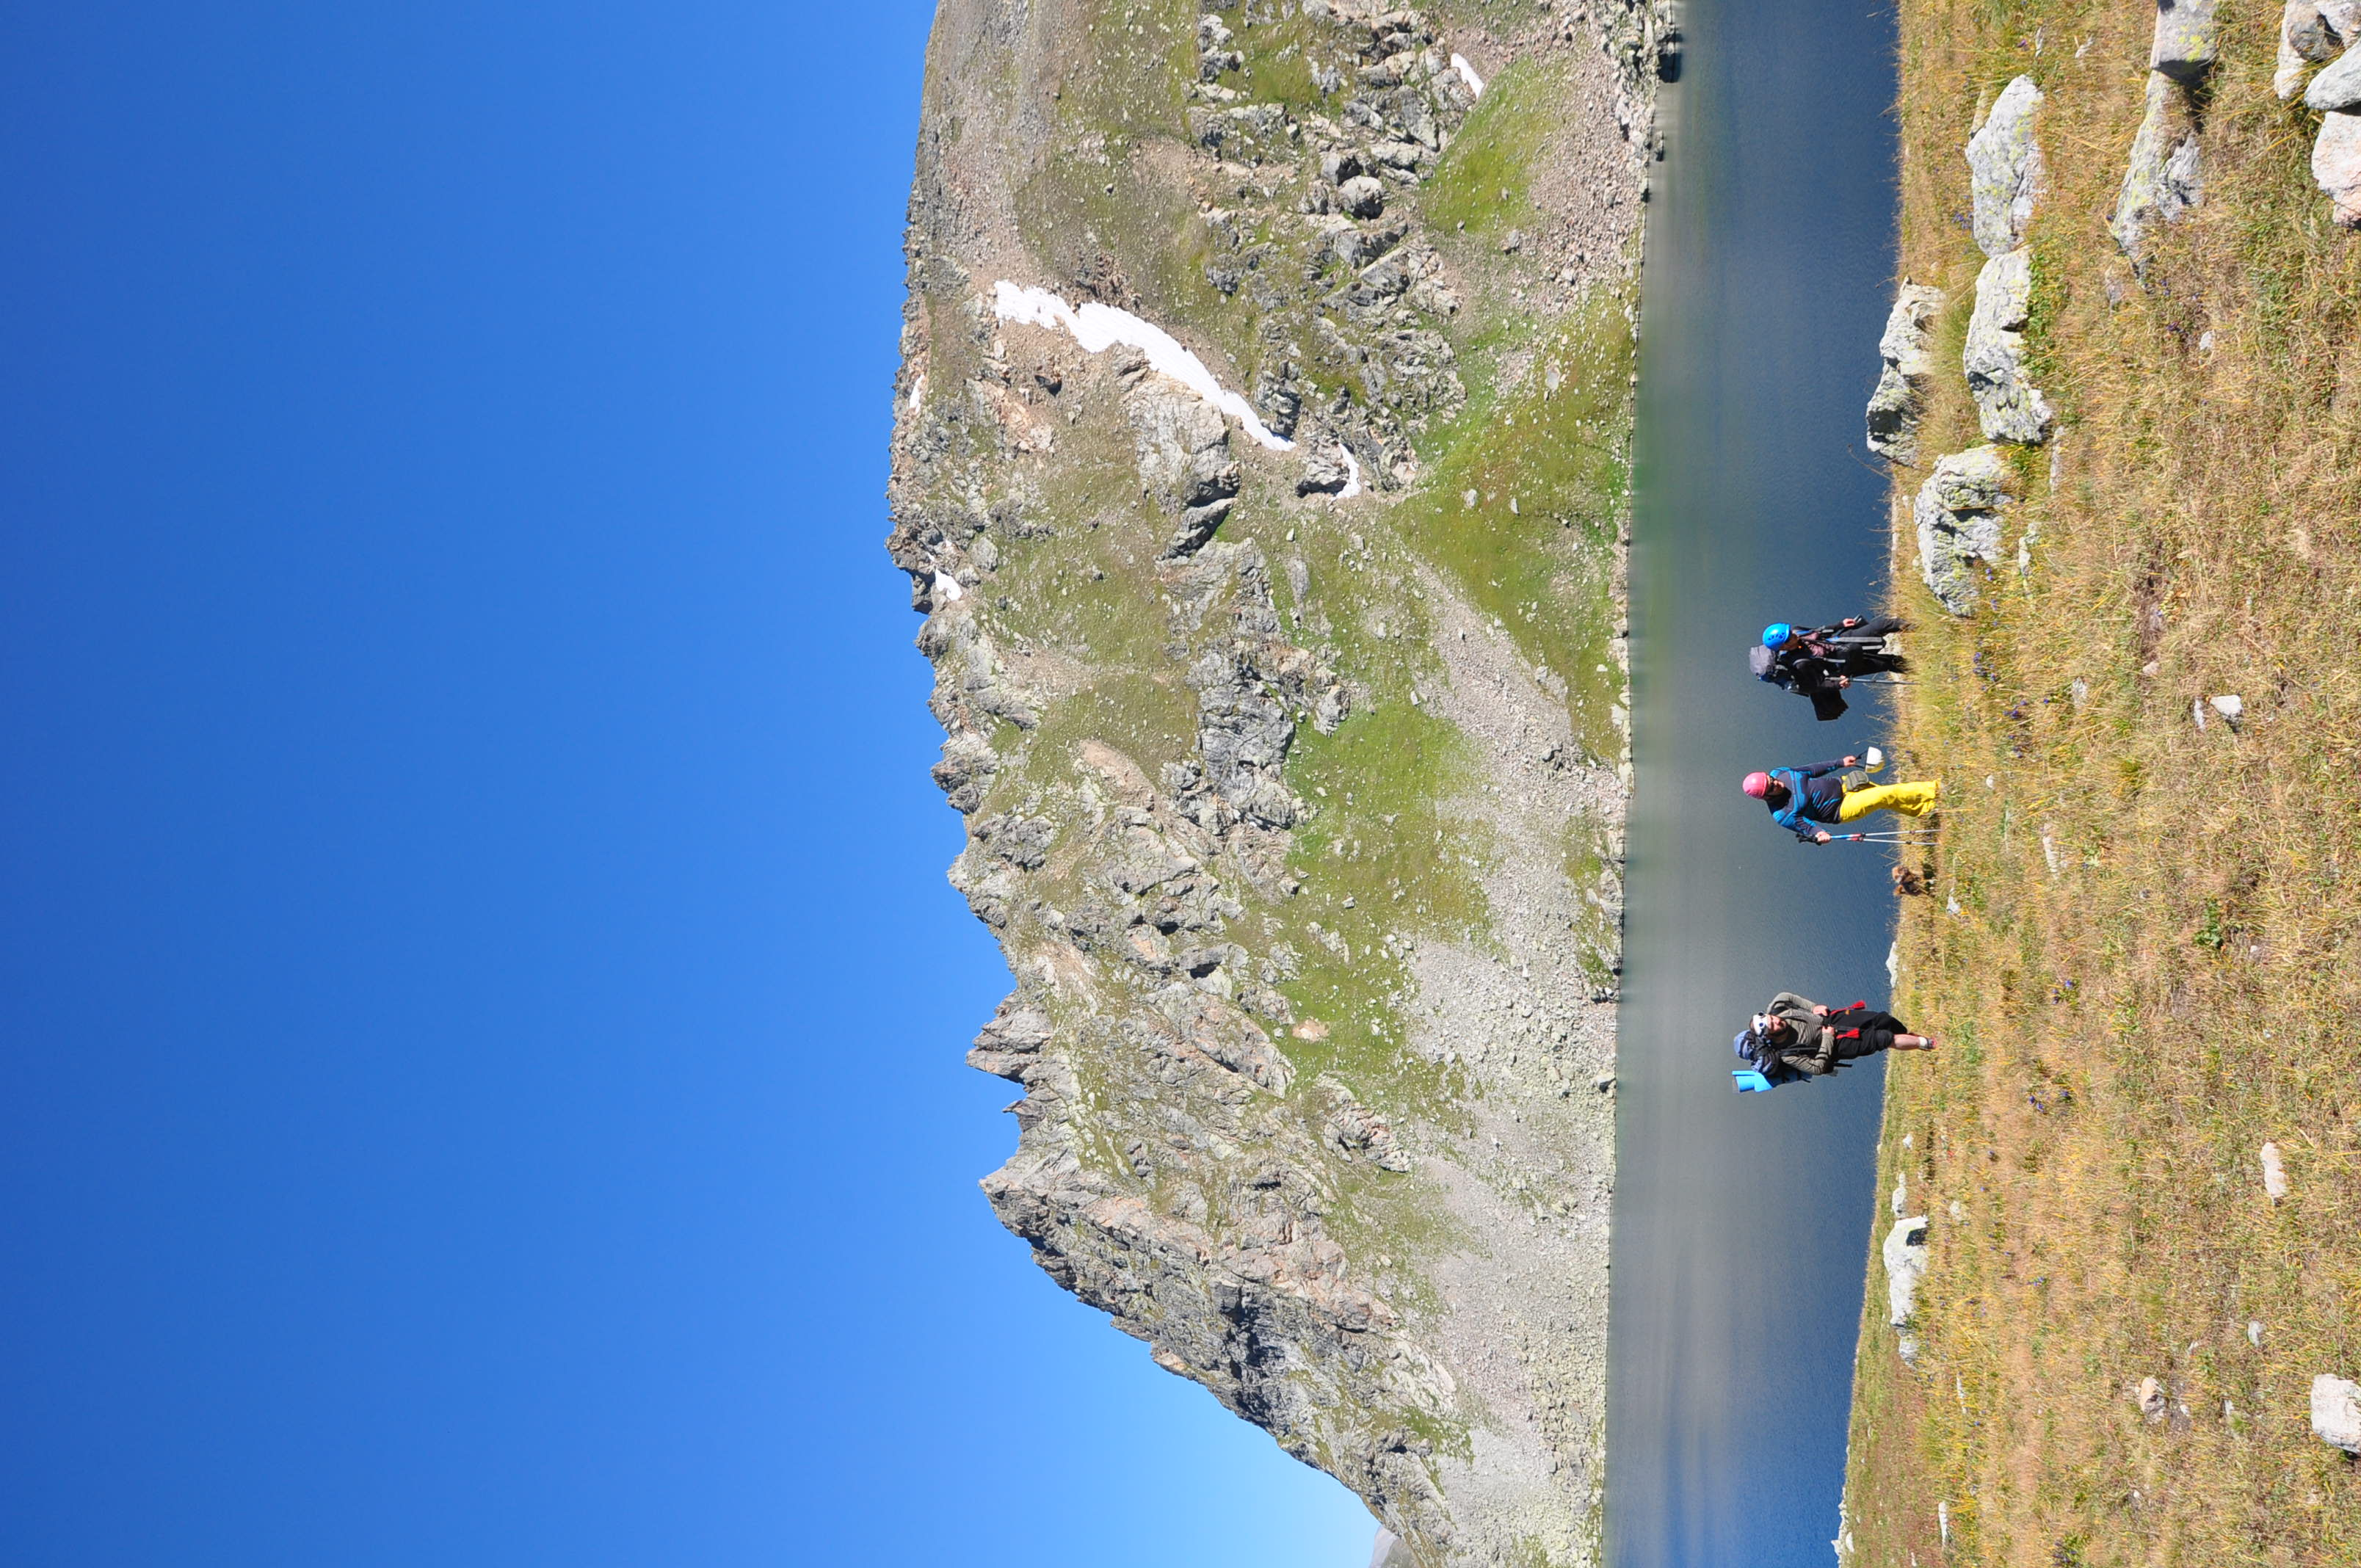
\includegraphics[width=0.65\linewidth]{../pics/DSC_0813}}
\end{frame}


\begin{frame}
	\frametitle{Дорога до озёр и далее на перевал}
	\framesubtitle{День 2, 19 августа}
	\centering
	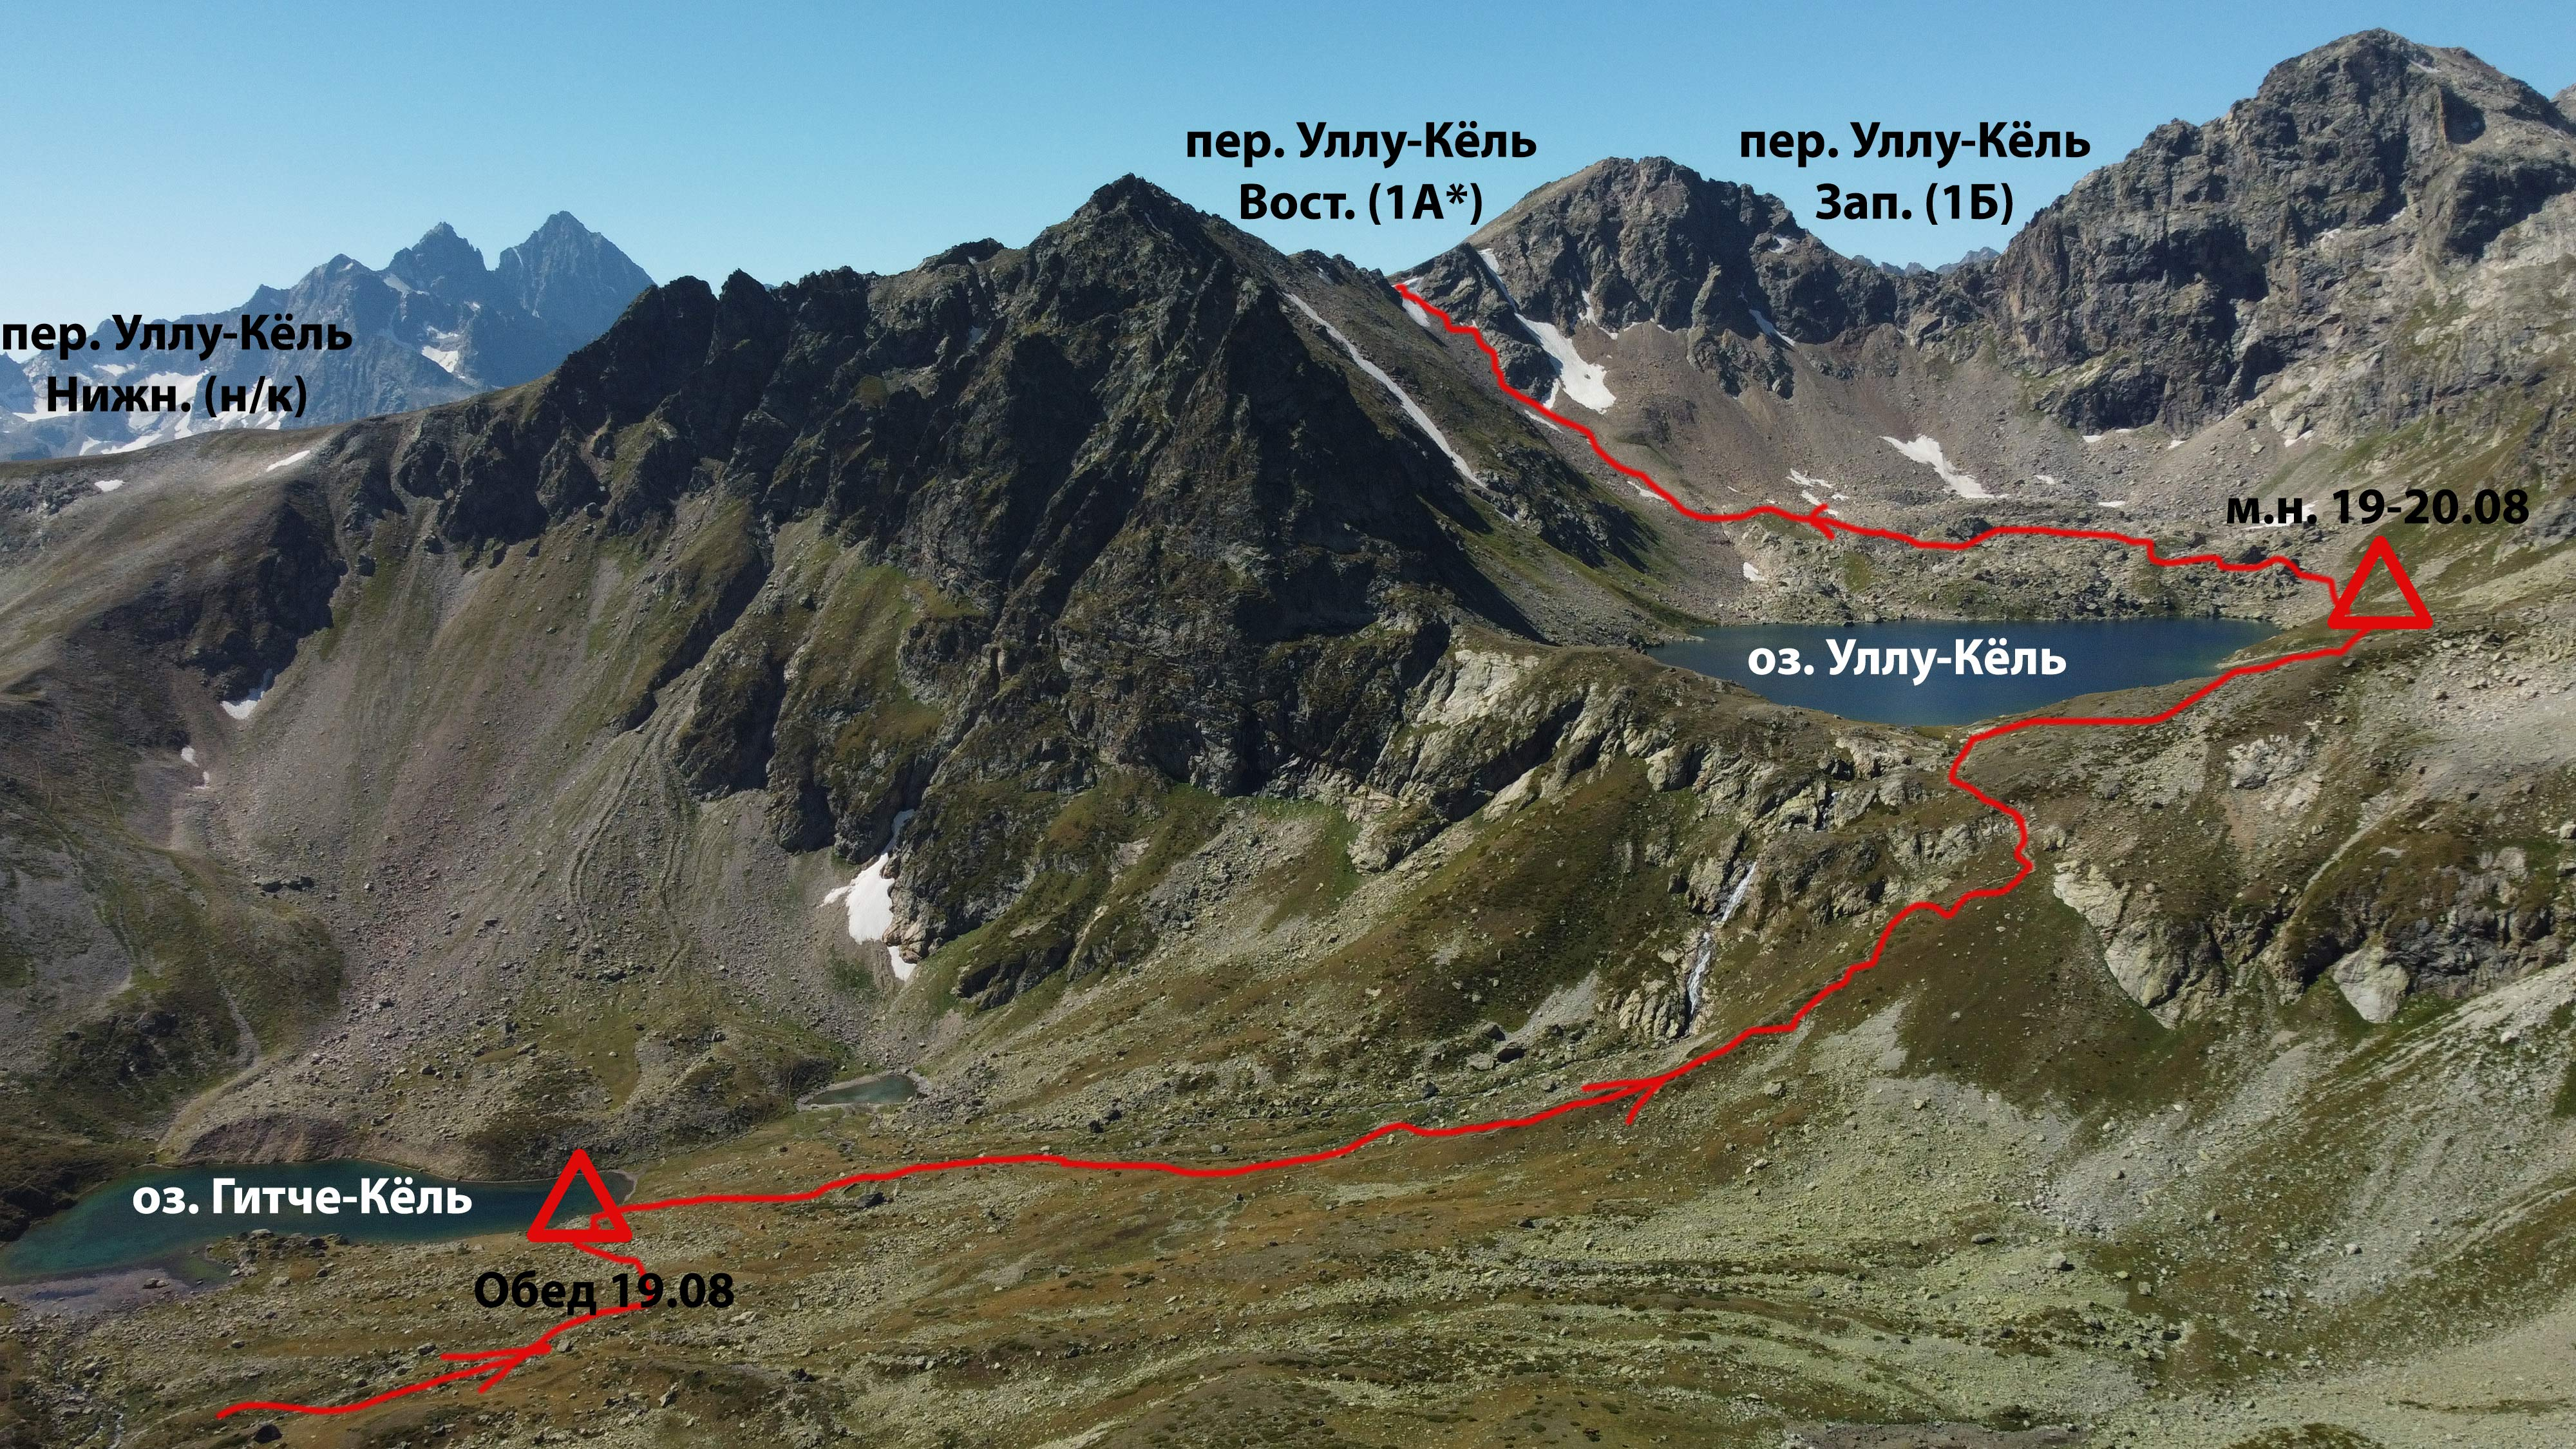
\includegraphics[width=\linewidth]{../pics/ullu_kuel_route}
\end{frame}
	\begin{frame}
	\frametitle{20 августа, день 3}
	{\tiny
		\begin{minipage}{\fourpicsize}
			\centering
			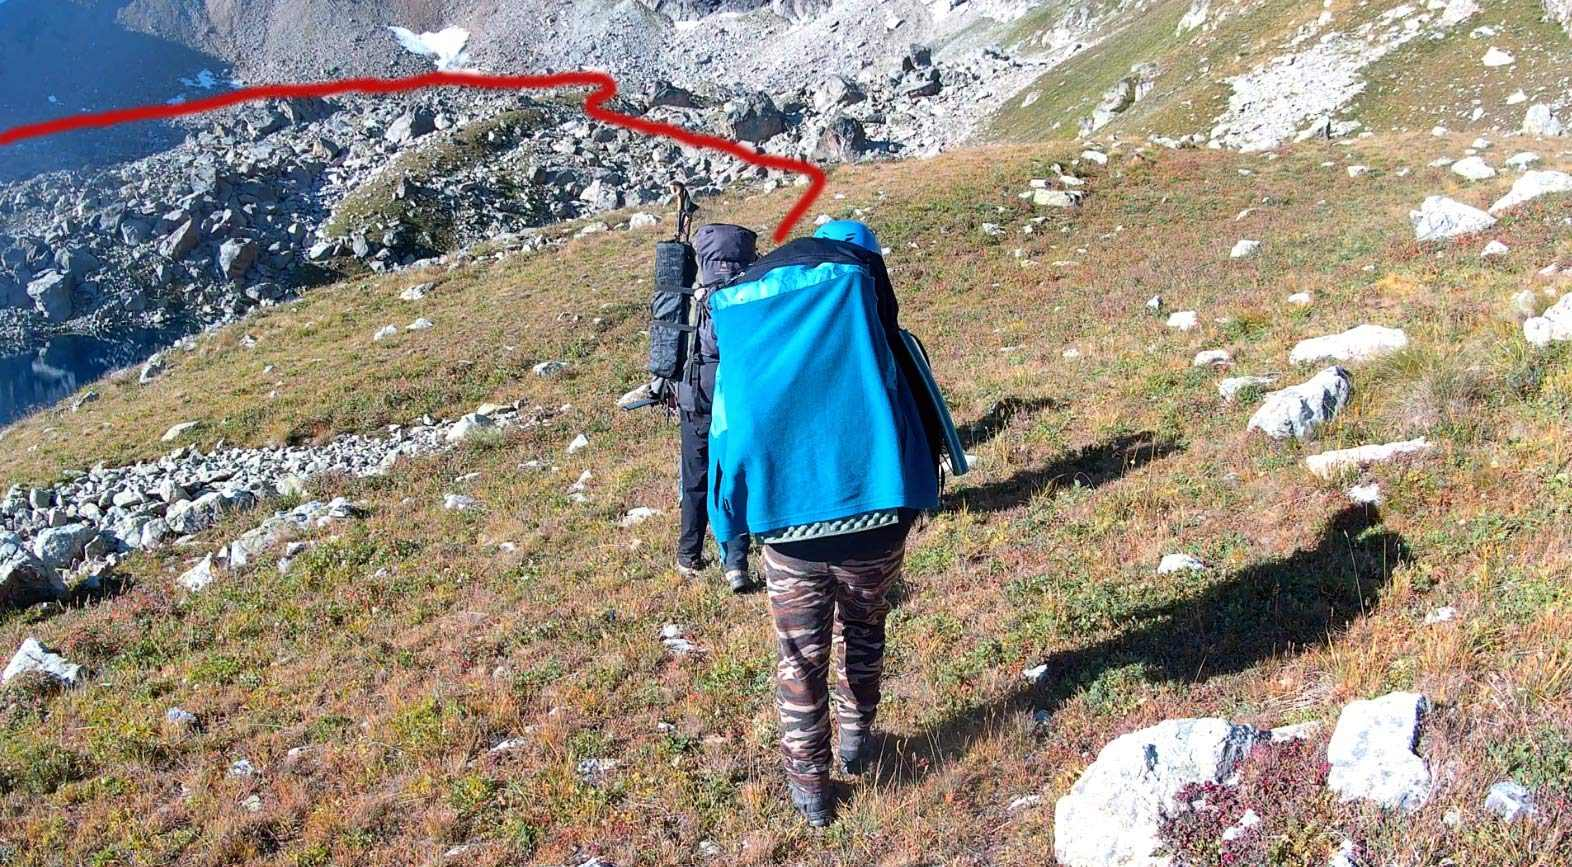
\includegraphics[width=\textwidth]{../pics/20aug1.jpg}			
			Движение к перевалу от м.н.
		\end{minipage}
		\hfill
		\begin{minipage}{\fourpicsize}
			\centering
			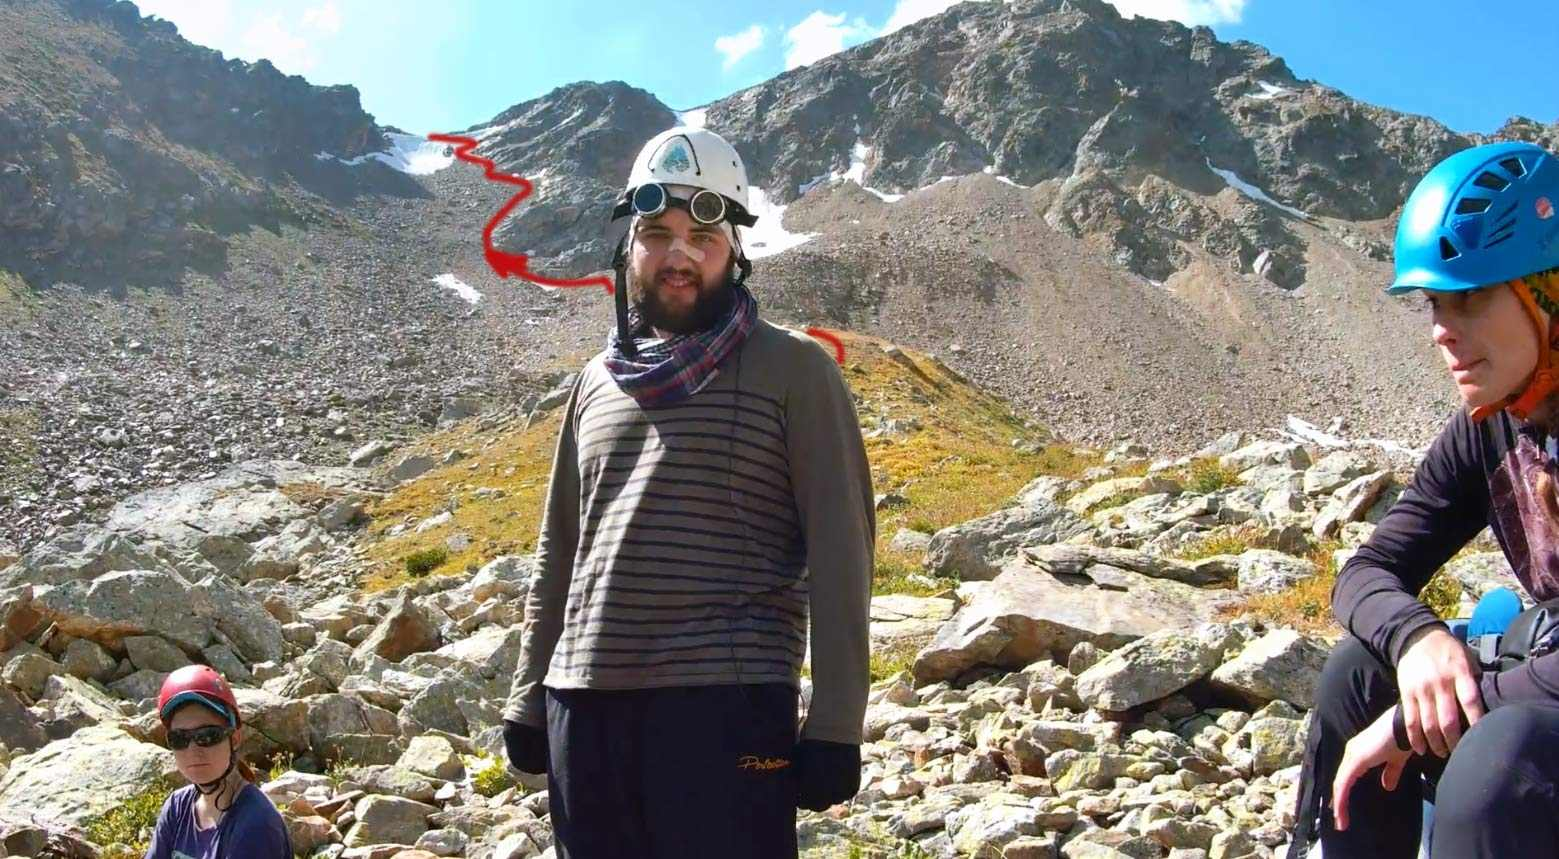
\includegraphics[width=\textwidth]{../pics/20aug2.jpg}			
			У взлёта
		\end{minipage}
		\vfill
		\begin{minipage}{\fourpicsize}
			\centering
			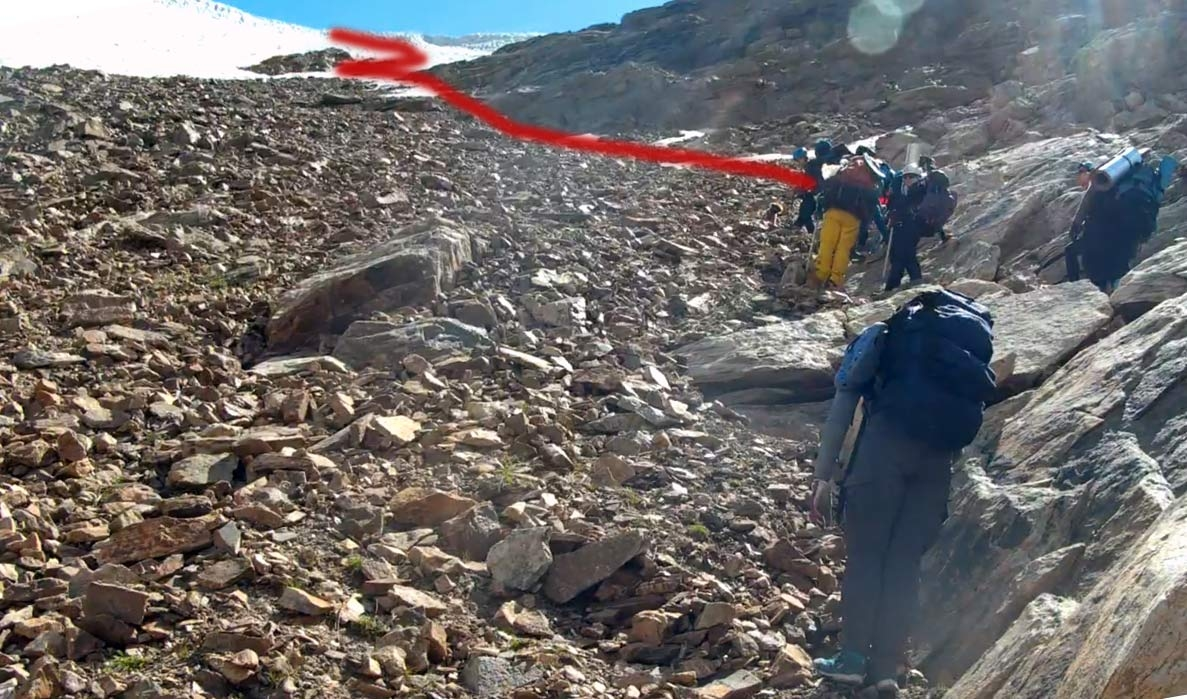
\includegraphics[width=\textwidth]{../pics/20aug3.jpg}			
			Идём по сыпухе		
		\end{minipage}
		\hfill
		\begin{minipage}{\fourpicsize}
			\centering
			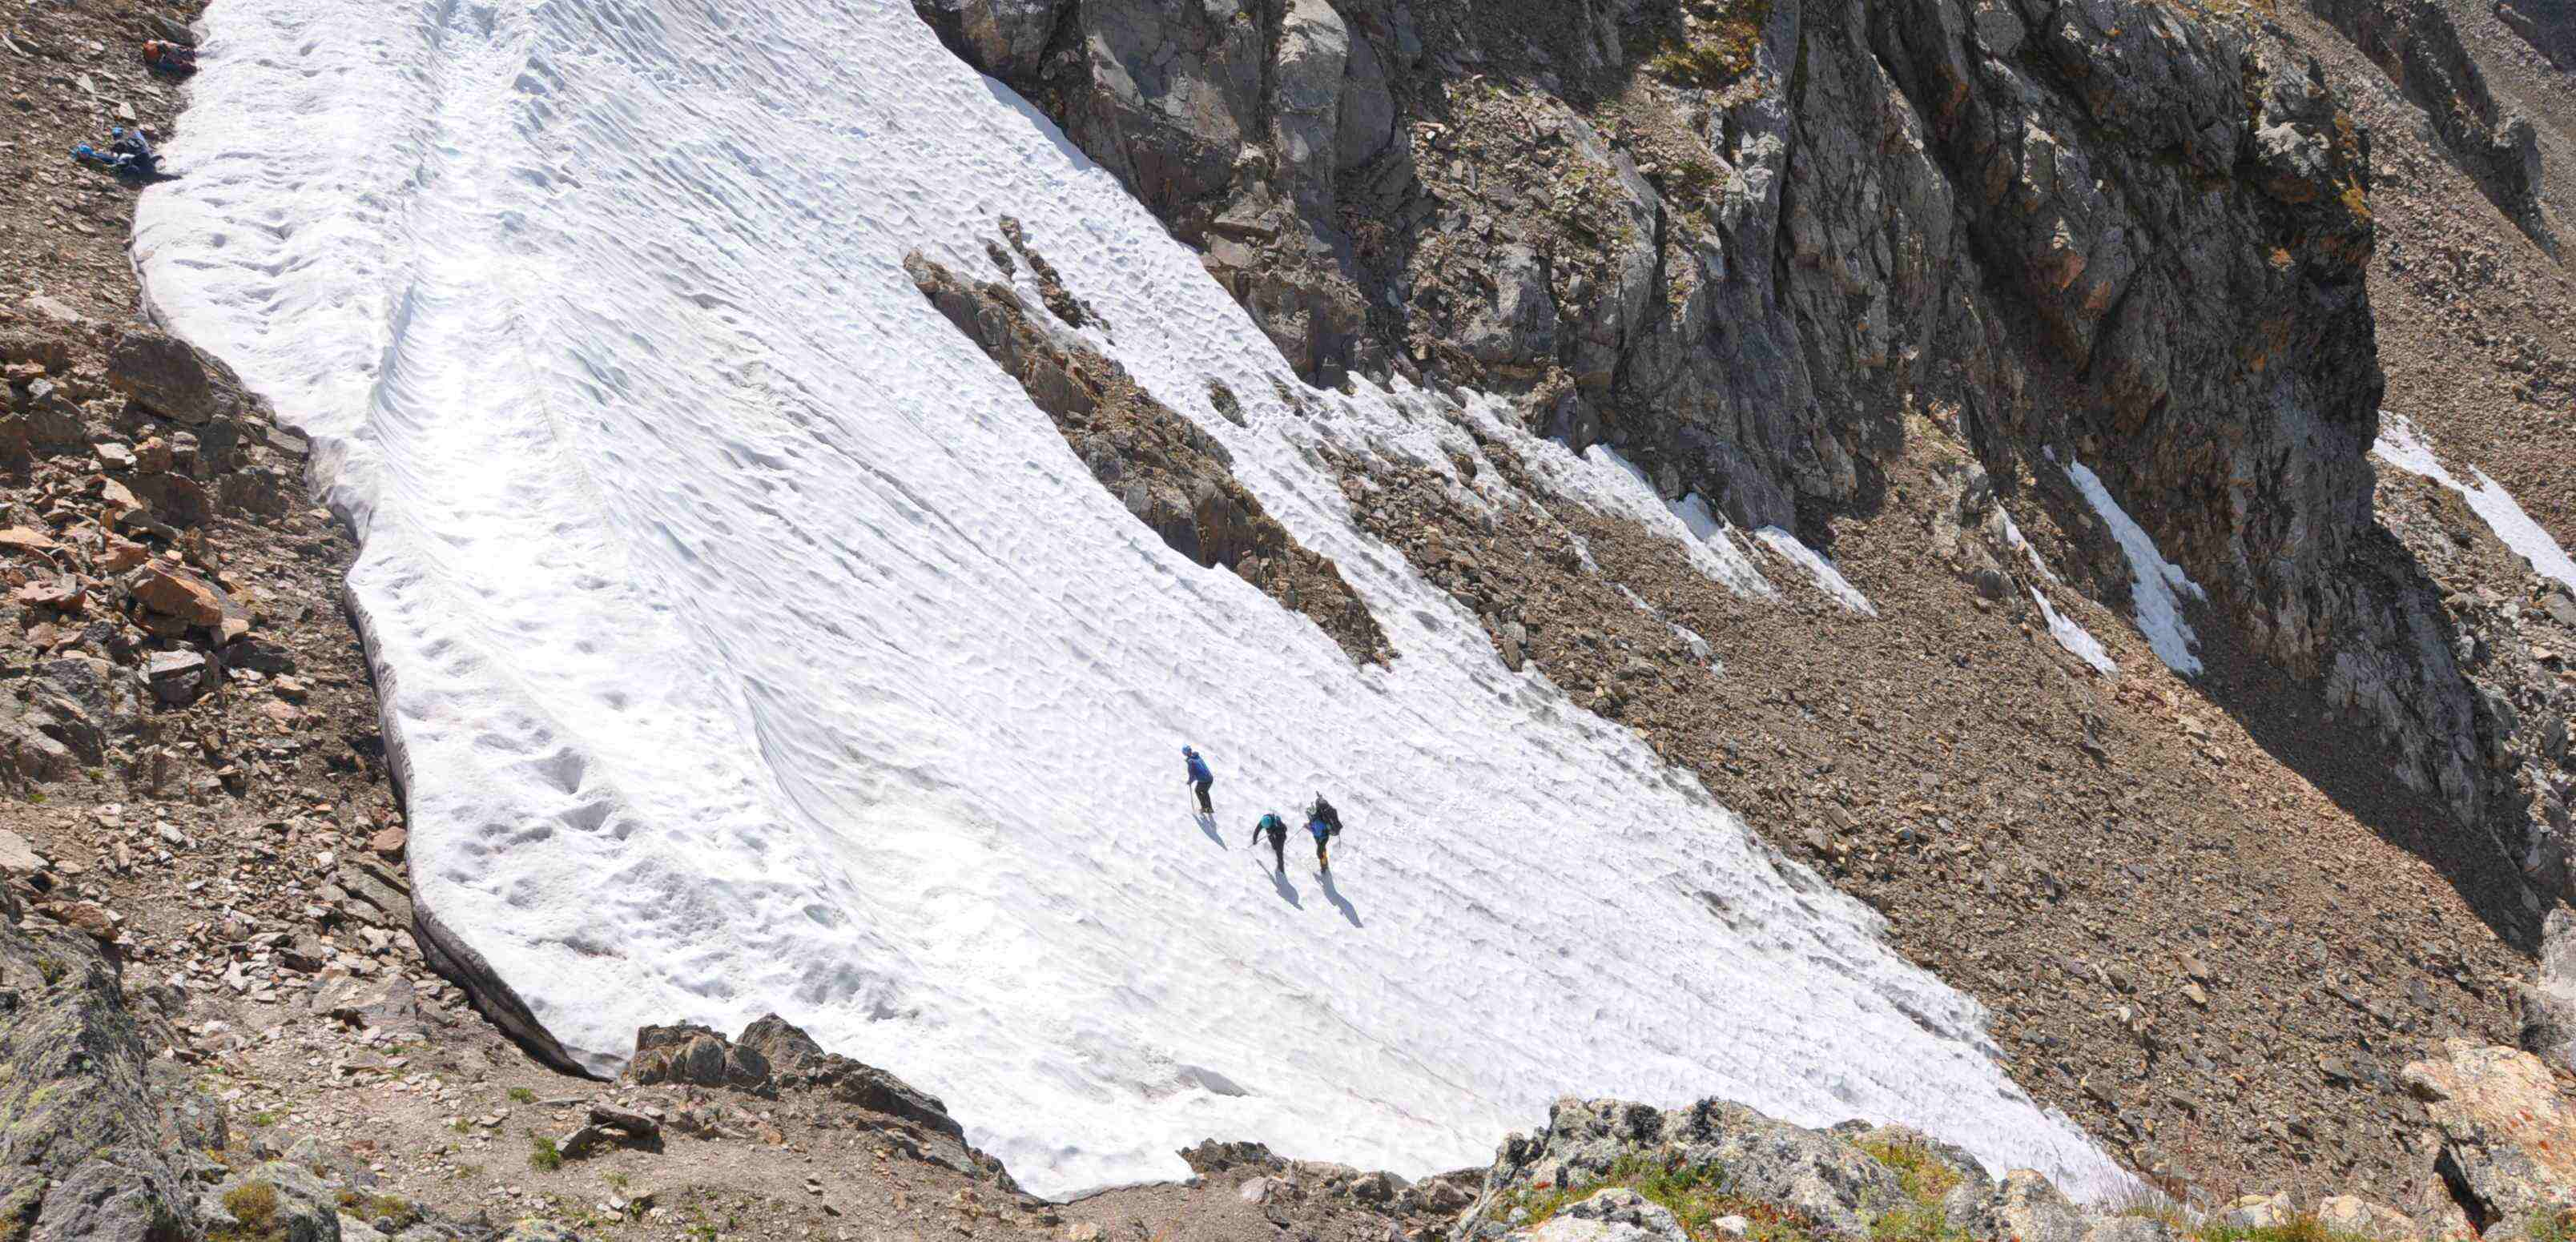
\includegraphics[width=\textwidth]{../pics/DSC_0946}			
			Маршрут движения группы по снежнику (красный), траектория срыва участника (синий), маршрут подъёма с сорвавшимся участником (чёрный)
		\end{minipage}
	}
\end{frame}
		\begin{frame}
	\frametitle{День 4. 21 августа}
	\framesubtitle{ т/б <<Глобус>>~--- д.р. Гондарай~--- д.р. Джалпаккол} % Optional subtitle
	\begin{columns}[c] % The "c" option specifies centered vertical alignment while the "t" option is used for top vertical alignment
		\begin{column}{0.45\textwidth} % Left column width
			\begin{itemize}
				\item Отдыхаем в «Глобусе»
				\item Непростое решение\texttrademark~№1
				\item Прошли \textbf{11.3} км
				\item ЧХВ: 3:54
				\item Набор/сброс: \textcolor{darkred}{\textbf{+390}}/\textcolor{darkblue}{\textbf{-225}}~м
			\end{itemize}
			
		\end{column}
		\begin{column}{0.5\textwidth} % Right column width
			\centering
			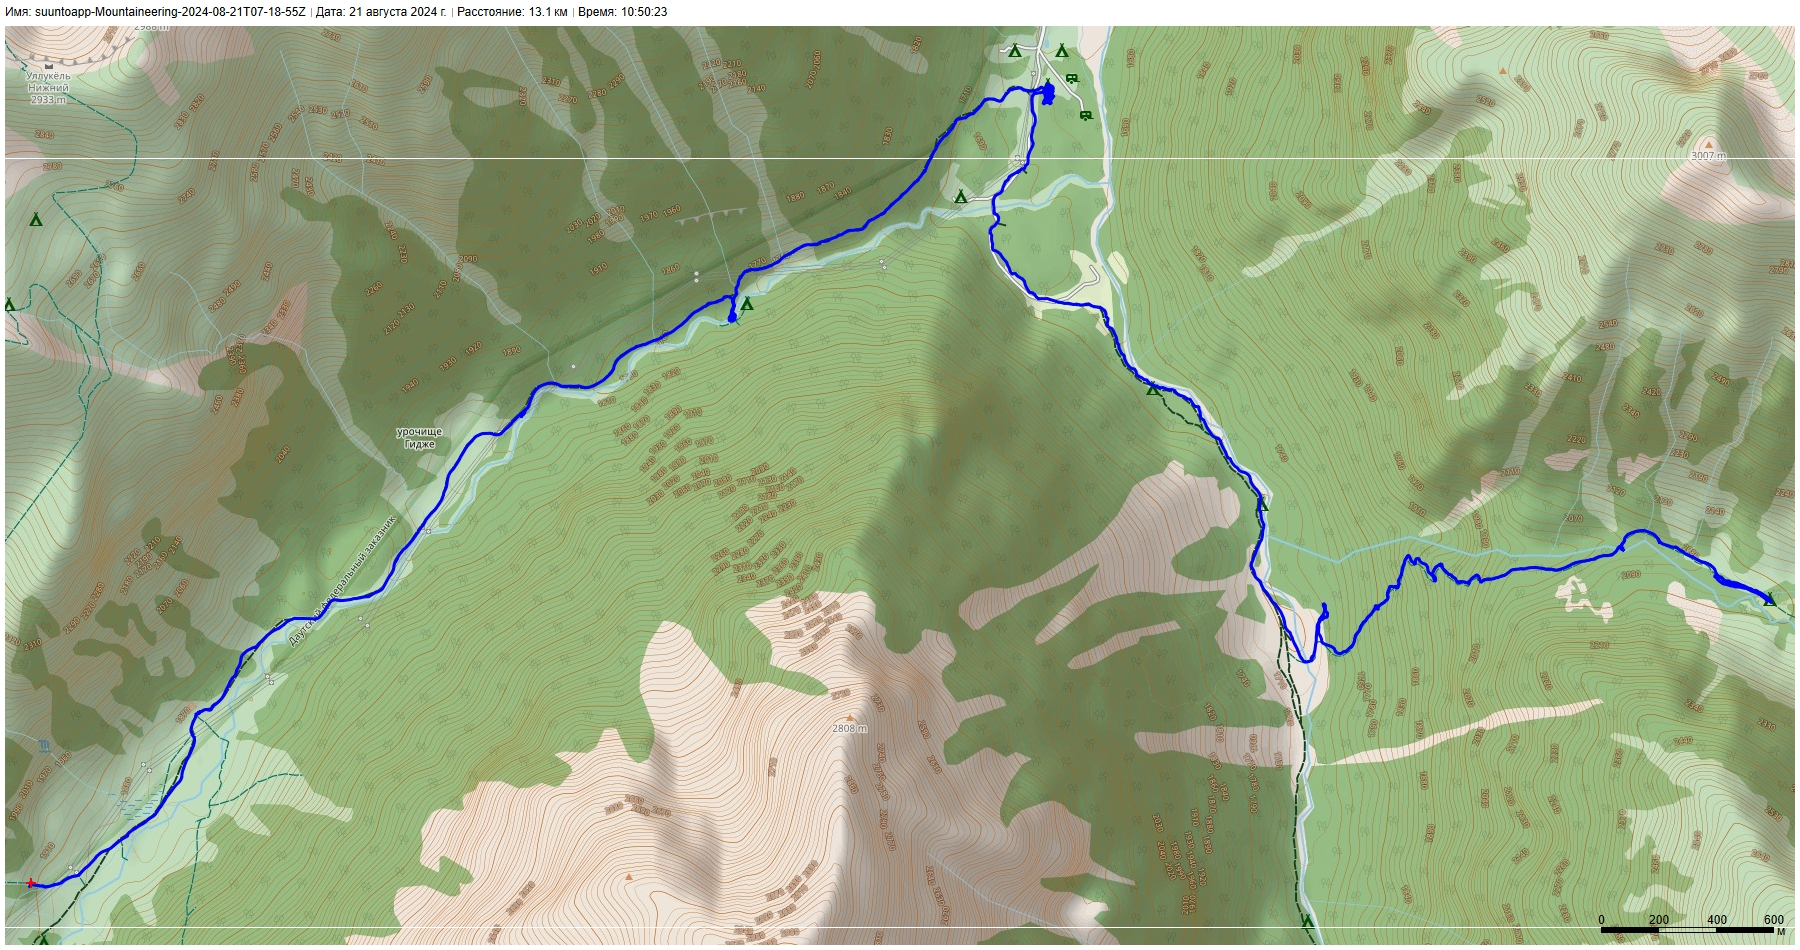
\includegraphics[width=\linewidth]{../pics/mini_maps/21}
		\end{column}
	\end{columns}
\end{frame}

\begin{frame}
	\frametitle{д.р. Махар}
	\framesubtitle{День 4, 21 августа}
	\centering
	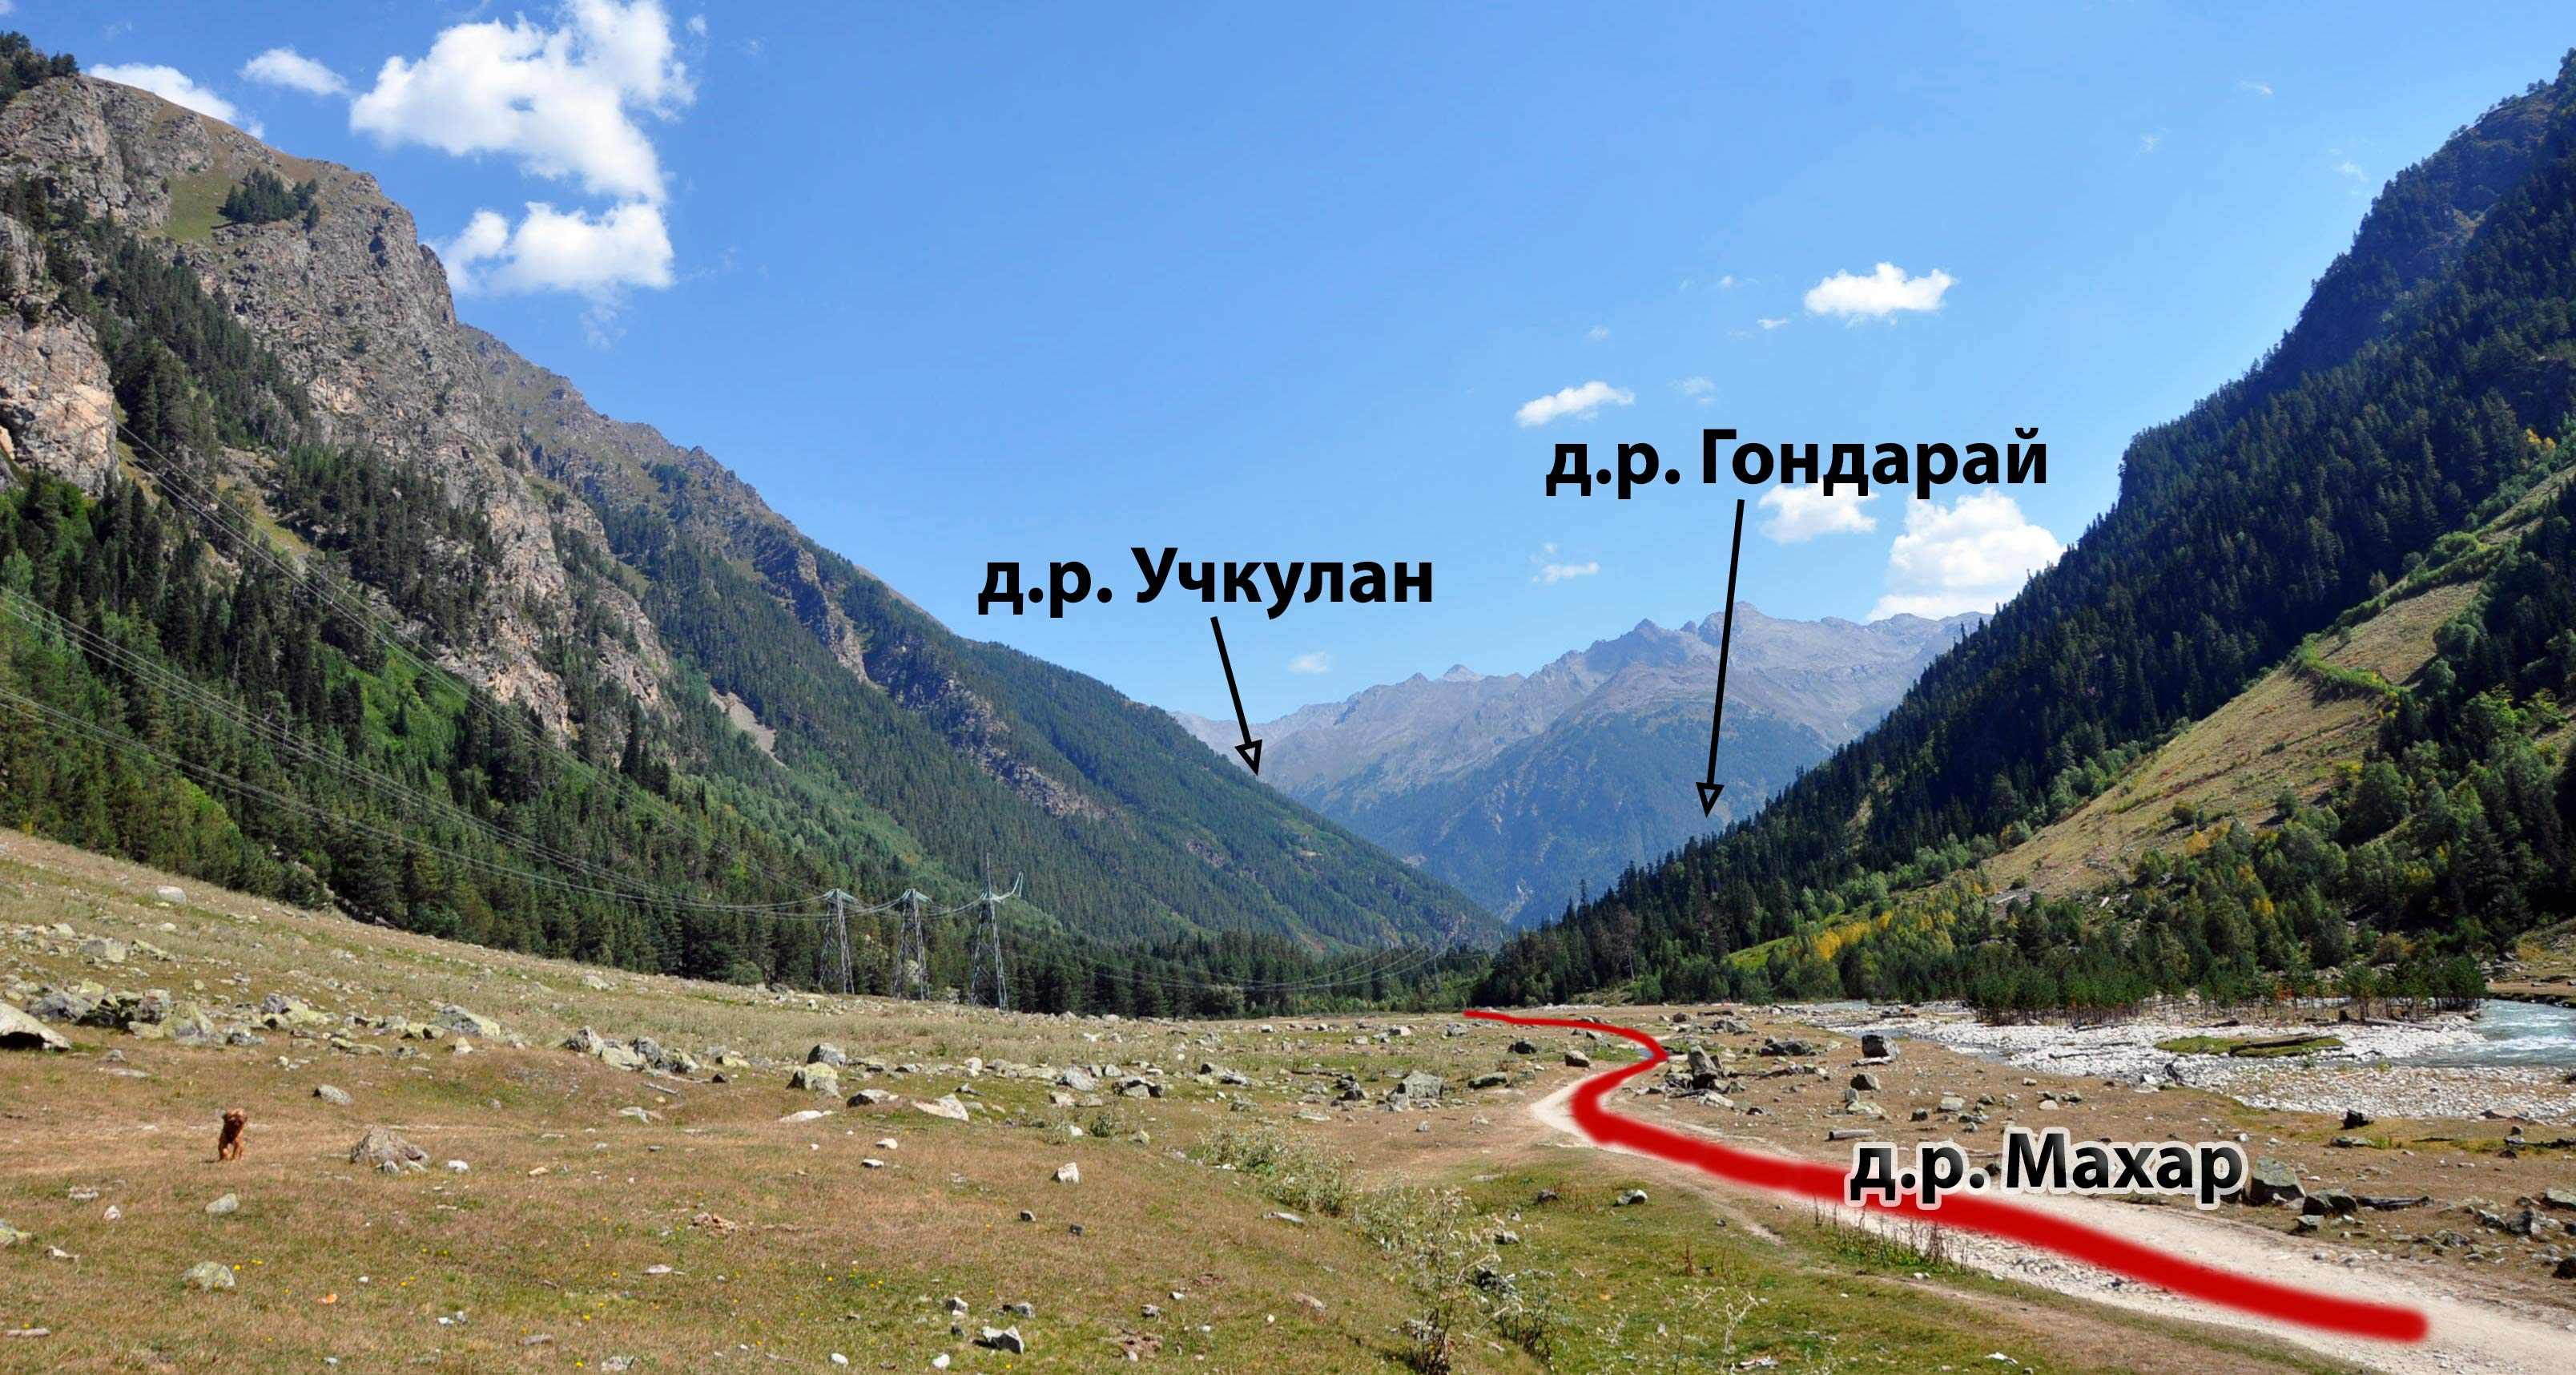
\includegraphics[width=\textwidth]{../pics/DSC_1003}			
\end{frame}

\begin{frame}
	\frametitle{Нарзанные источники}
	\framesubtitle{День 4, 21 августа}
	{\tiny
		\begin{minipage}{\fourpicsize}
			\centering
			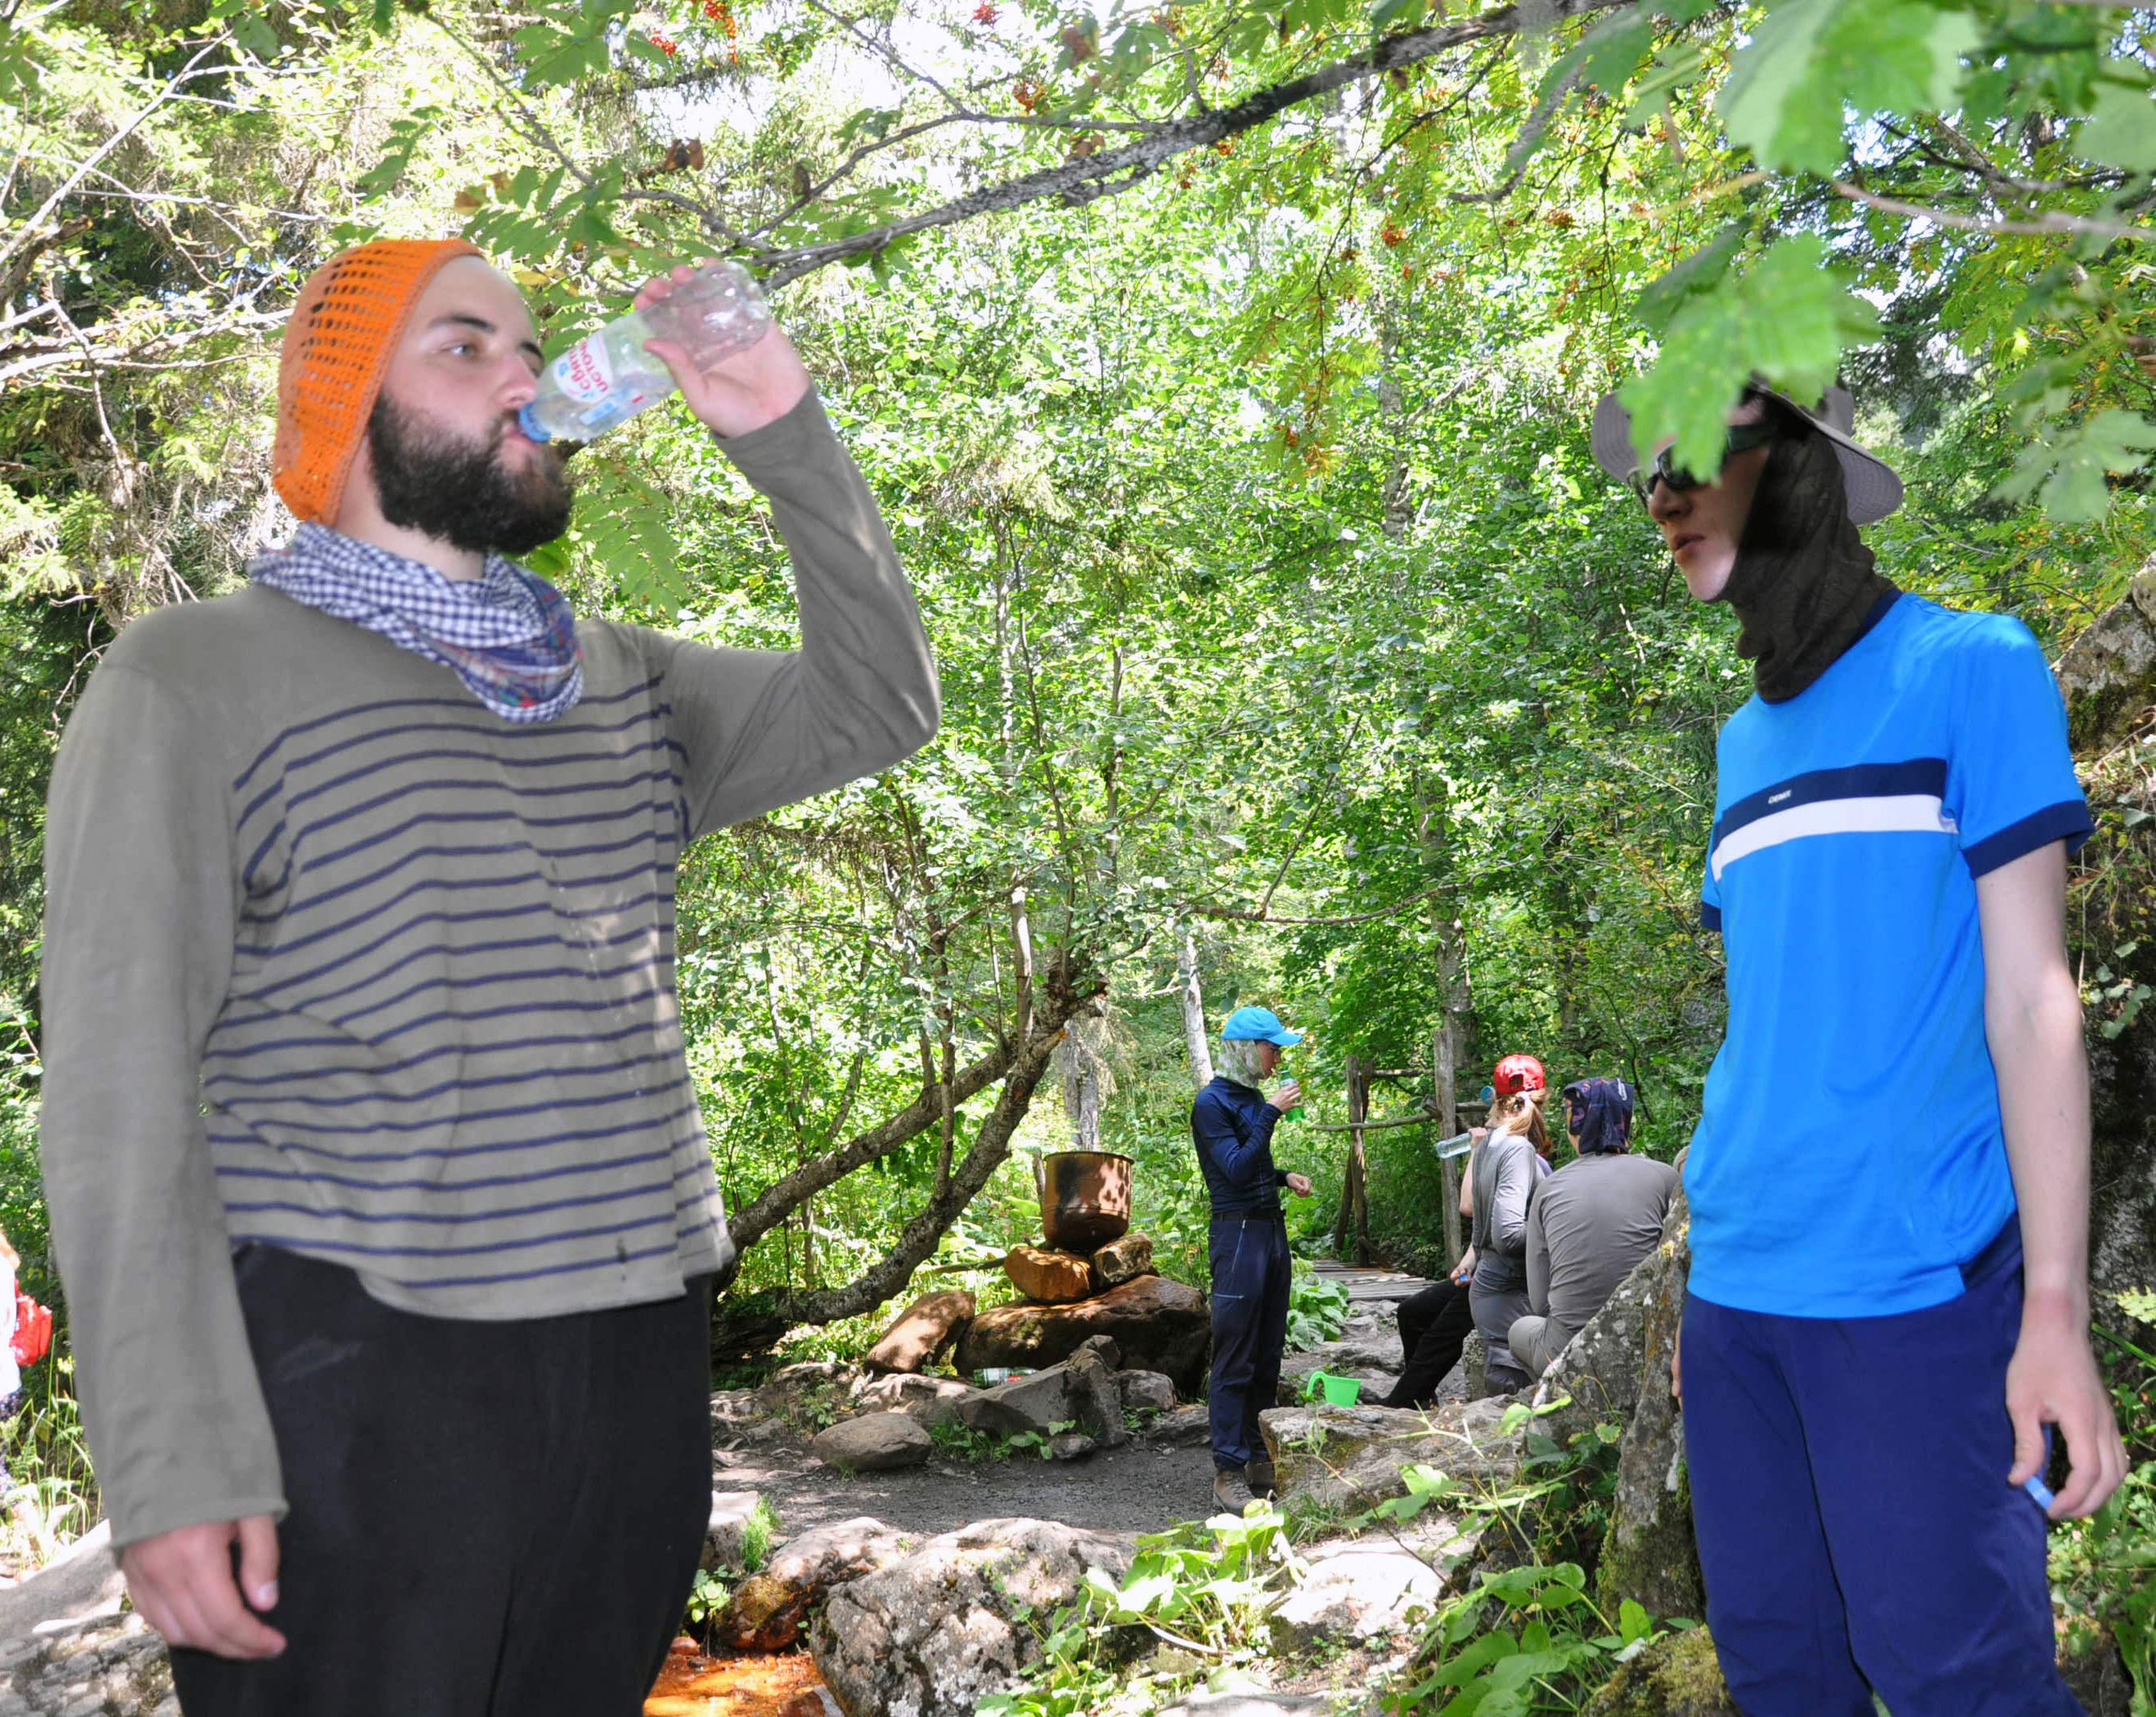
\includegraphics[width=\textwidth]{../pics/DSC_1043}			
		\end{minipage}
		\hfill
		\begin{minipage}{\fourpicsize}
			\centering
			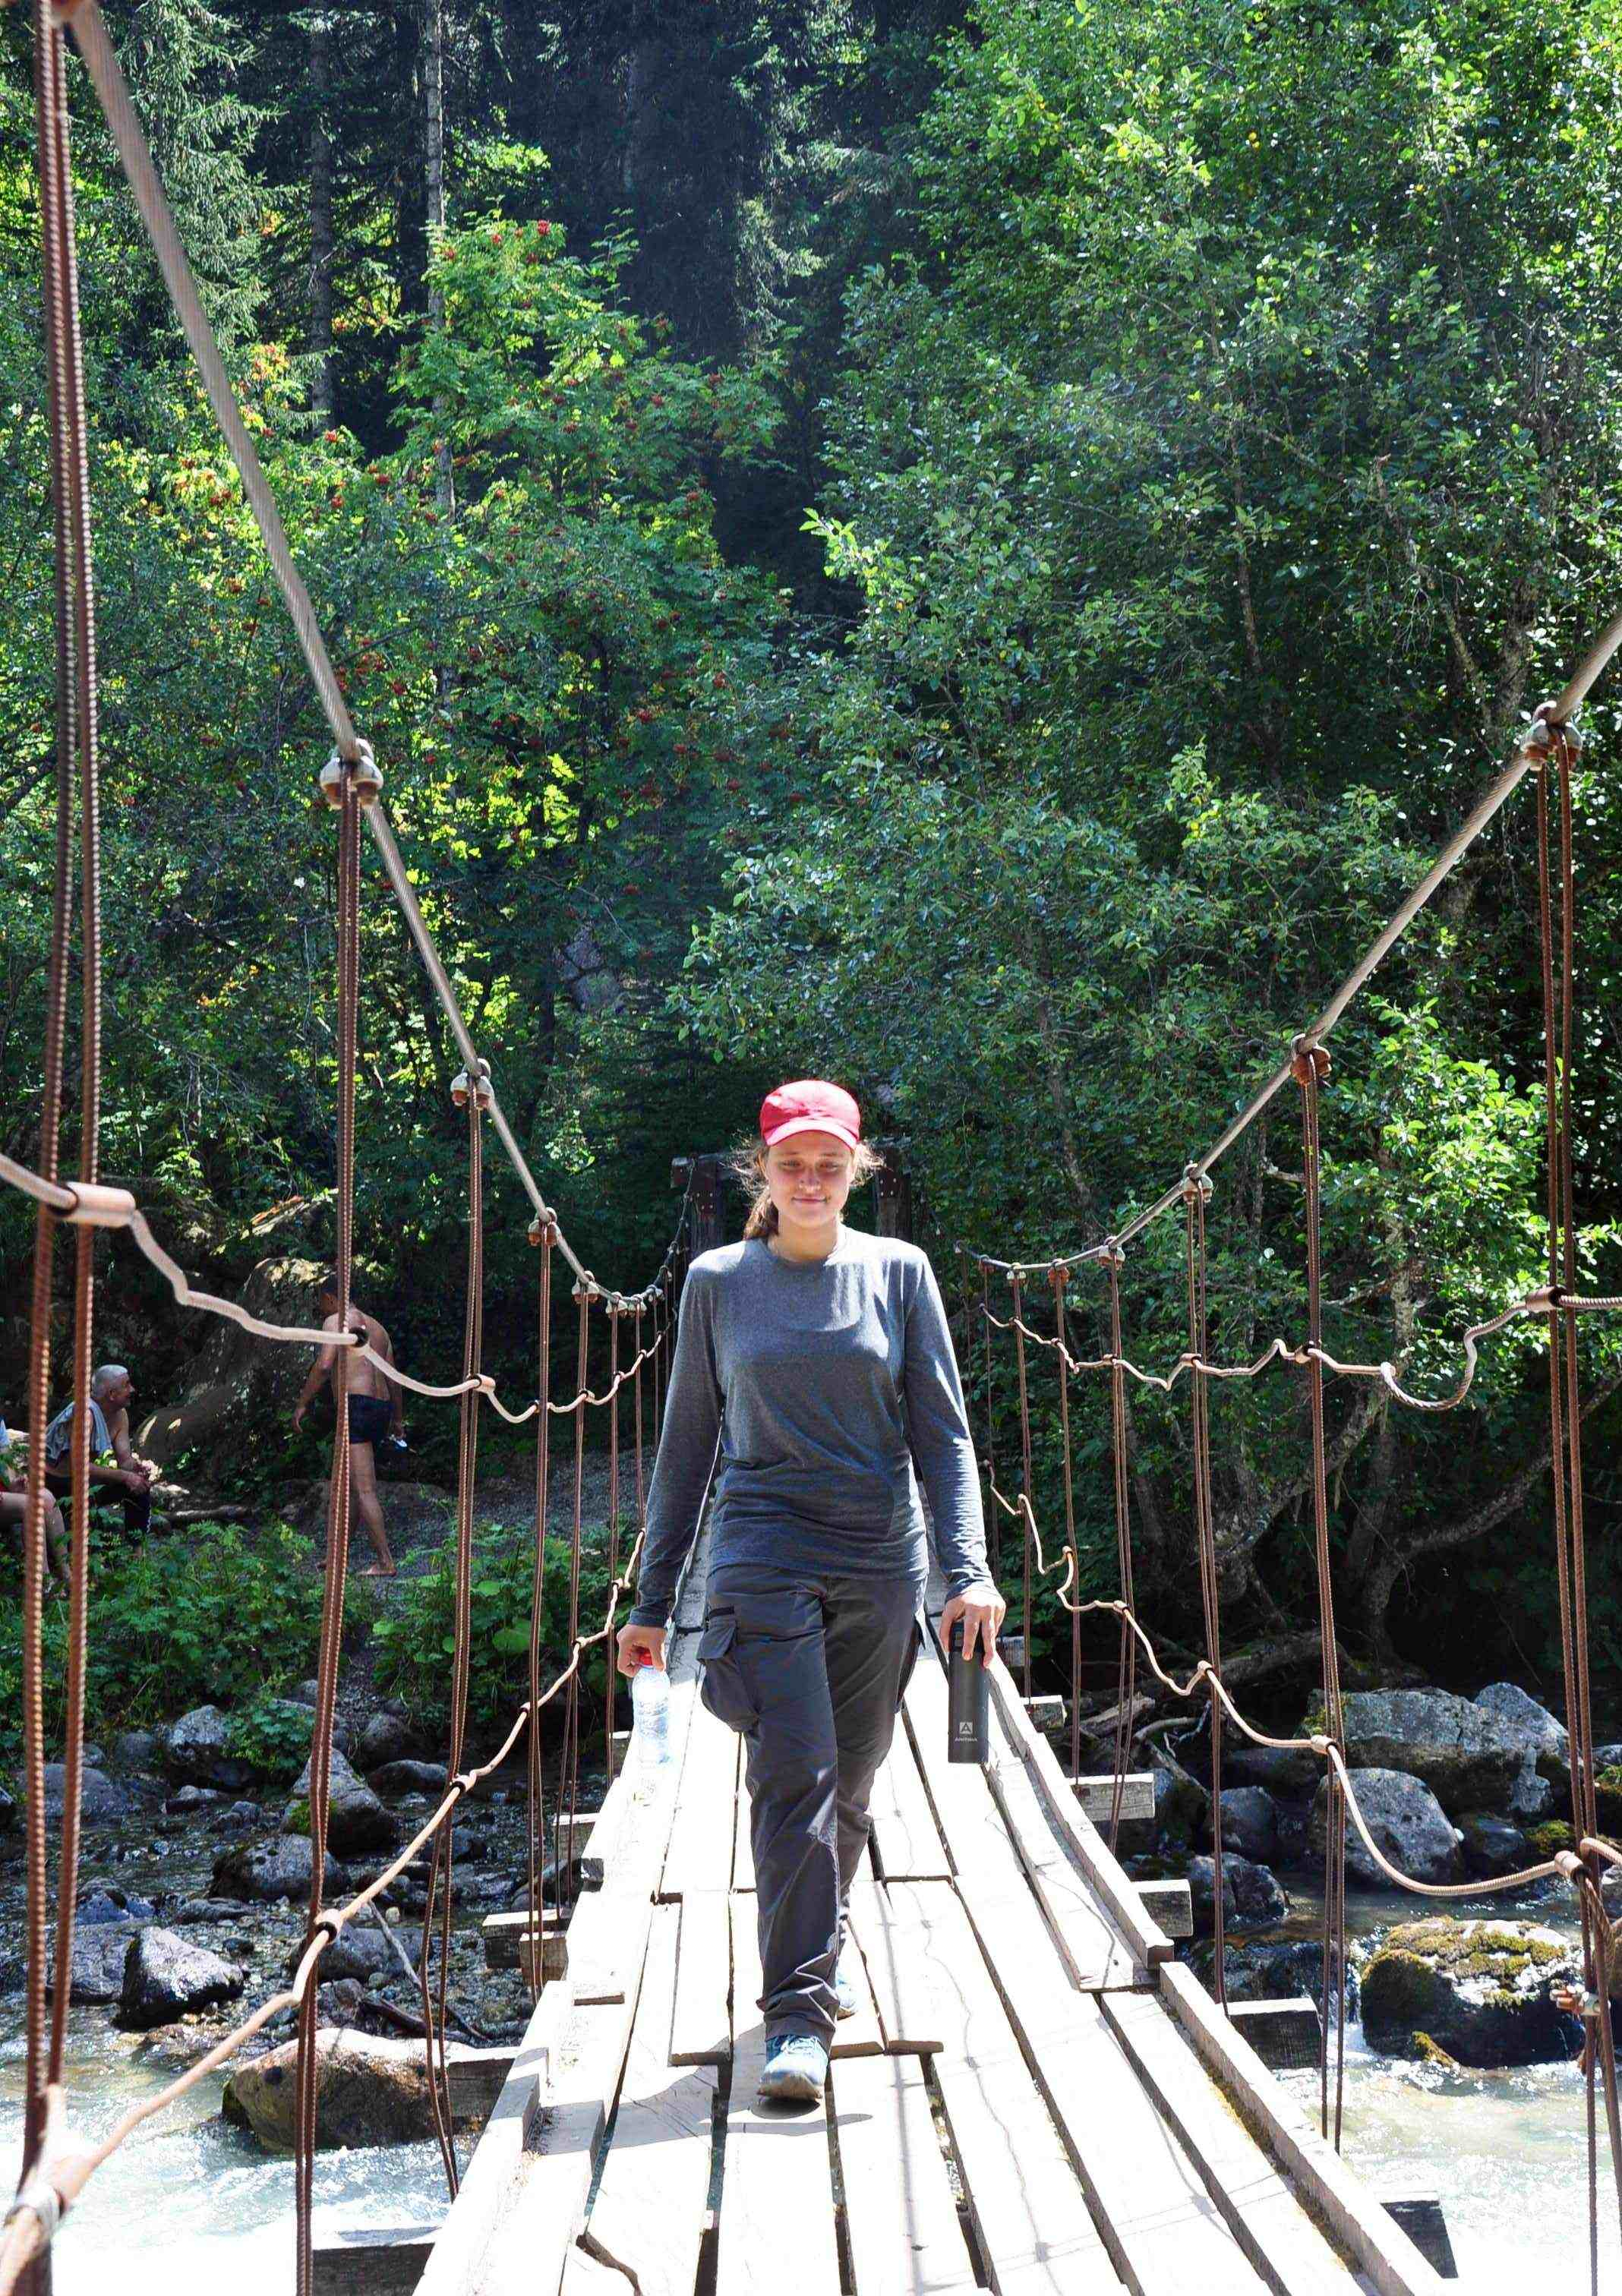
\includegraphics[width=0.8\textwidth]{../pics/DSC_1098}			
		\end{minipage}
		\vfill
	}
\end{frame}

\begin{frame}
	\frametitle{Учимся утилизировать использованные газовые баллоны \smiley}
	\framesubtitle{День 4, 21 августа}
	{\tiny
		\begin{minipage}{\fourpicsize}
			\centering
			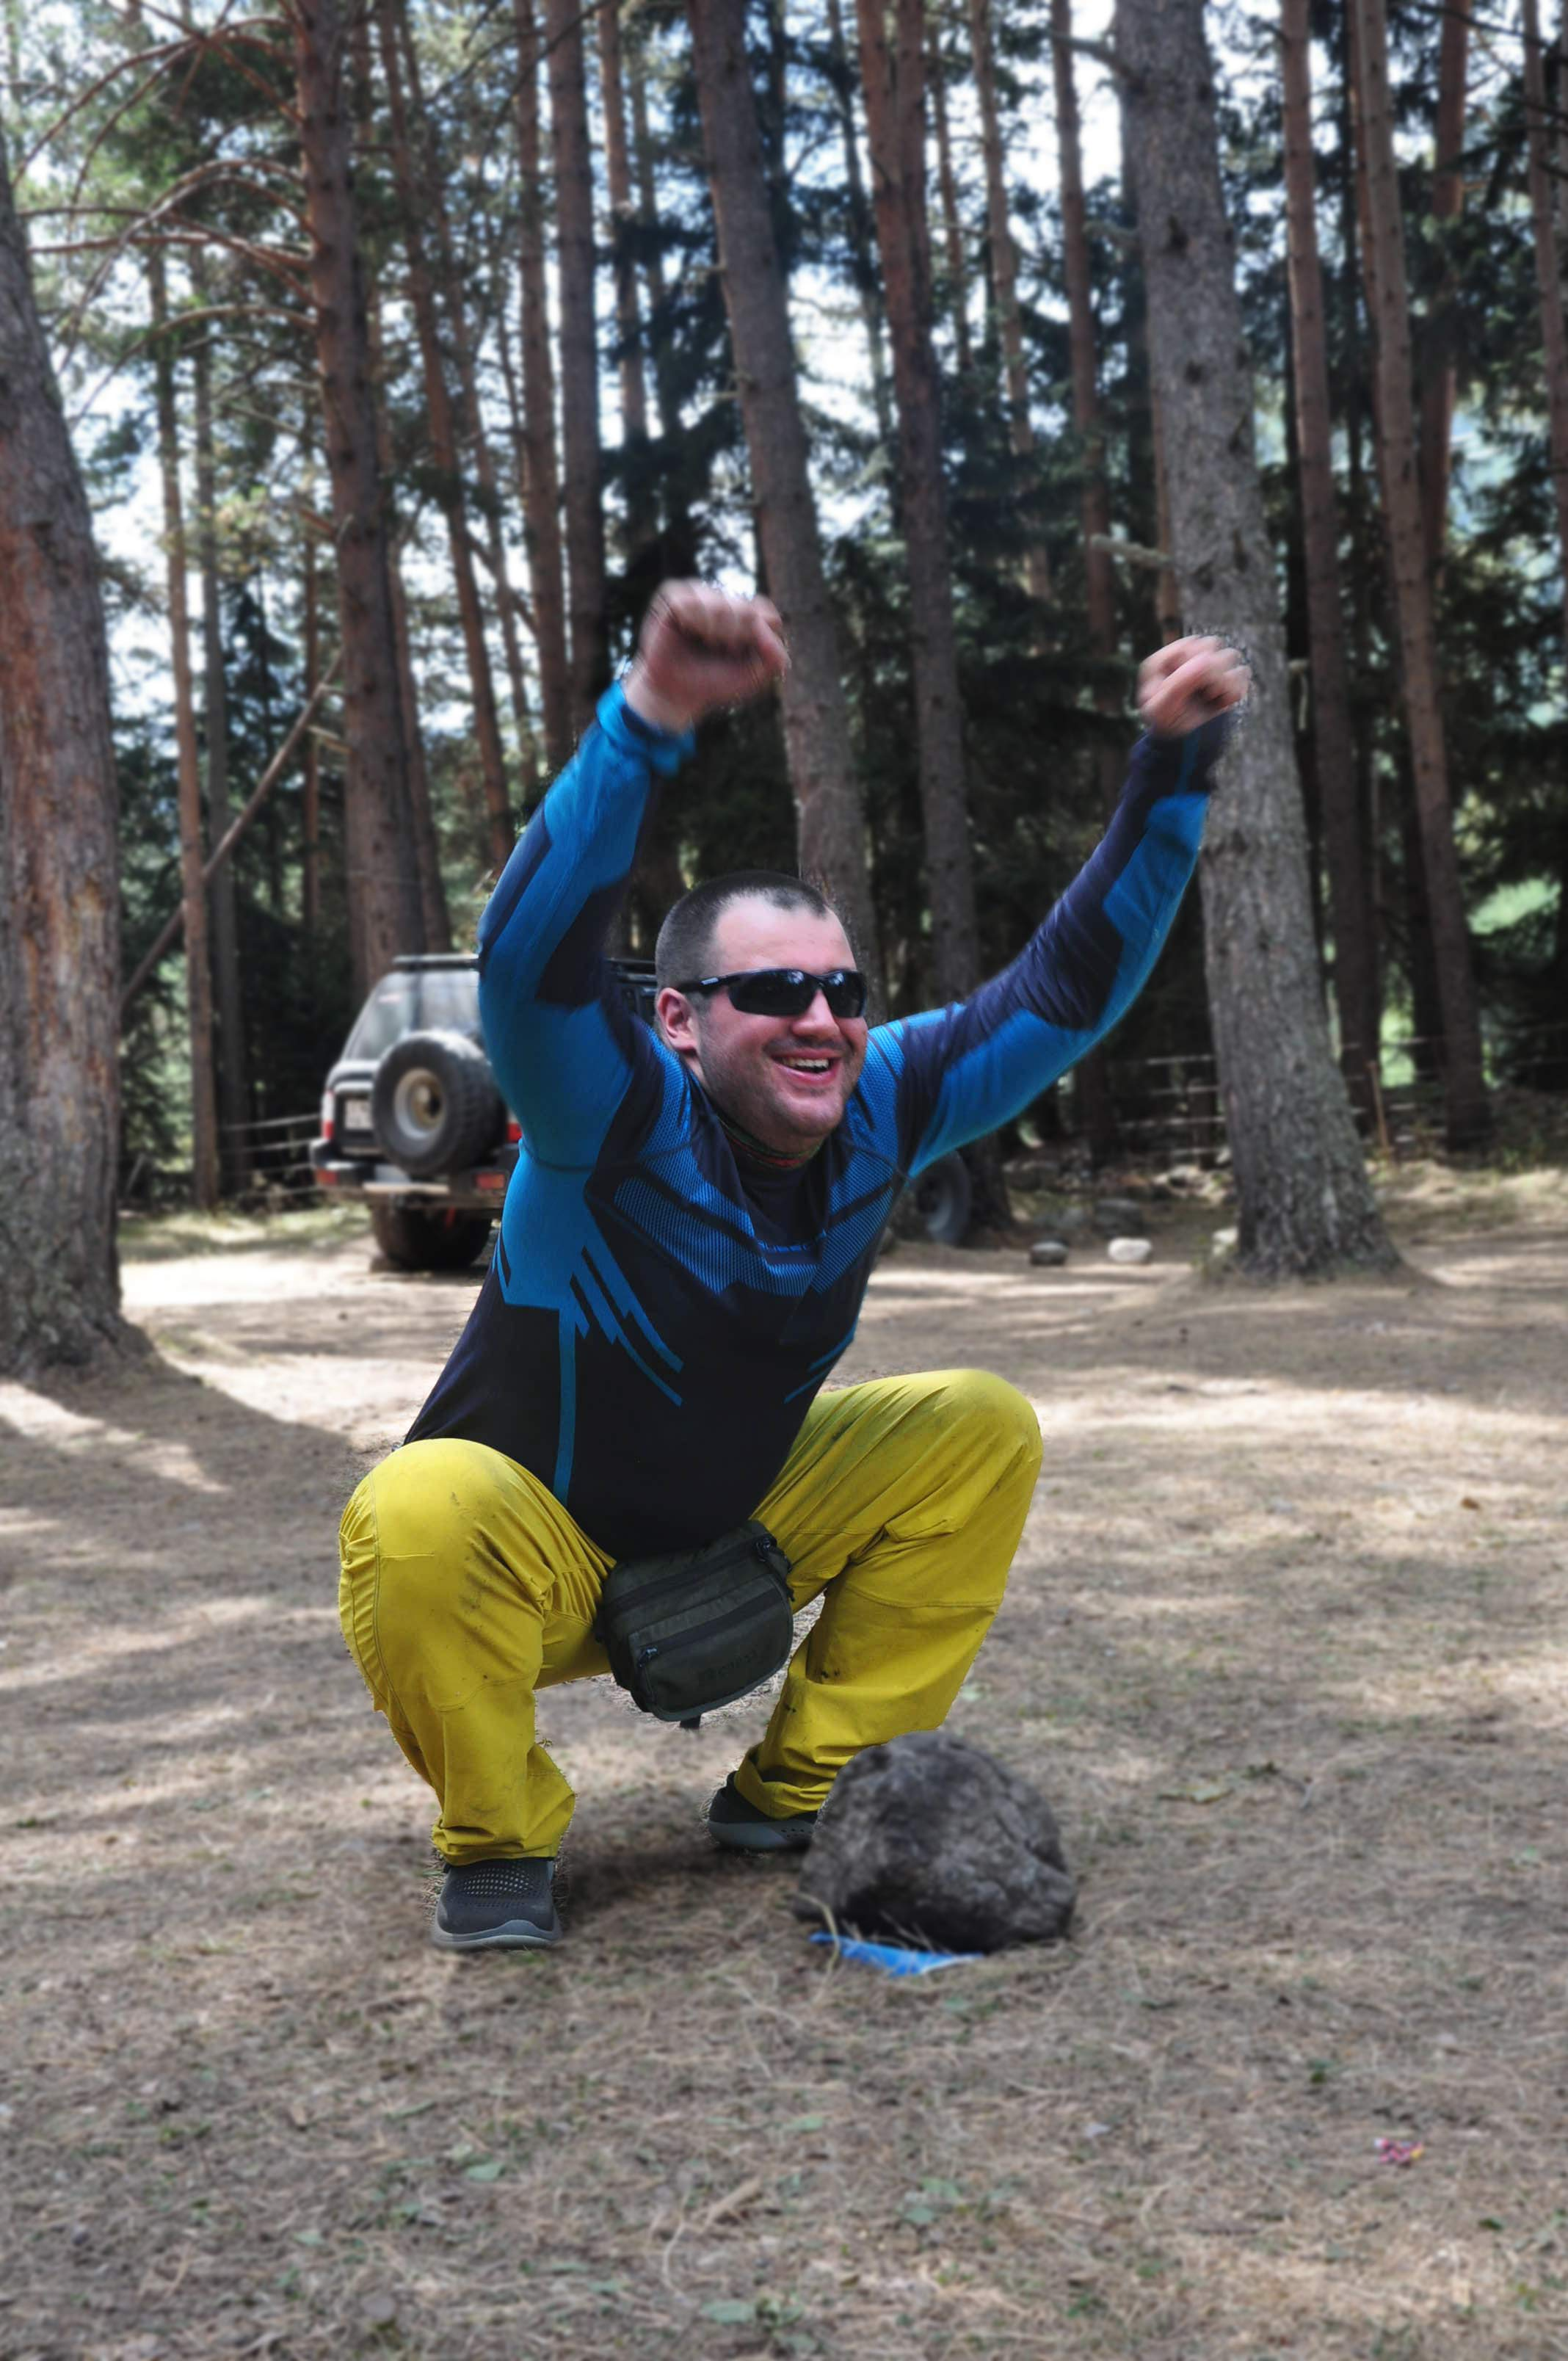
\includegraphics[width=\textwidth]{../pics/DSC_1150}			
		\end{minipage}
		\hfill
		\begin{minipage}{\fourpicsize}
			\centering
			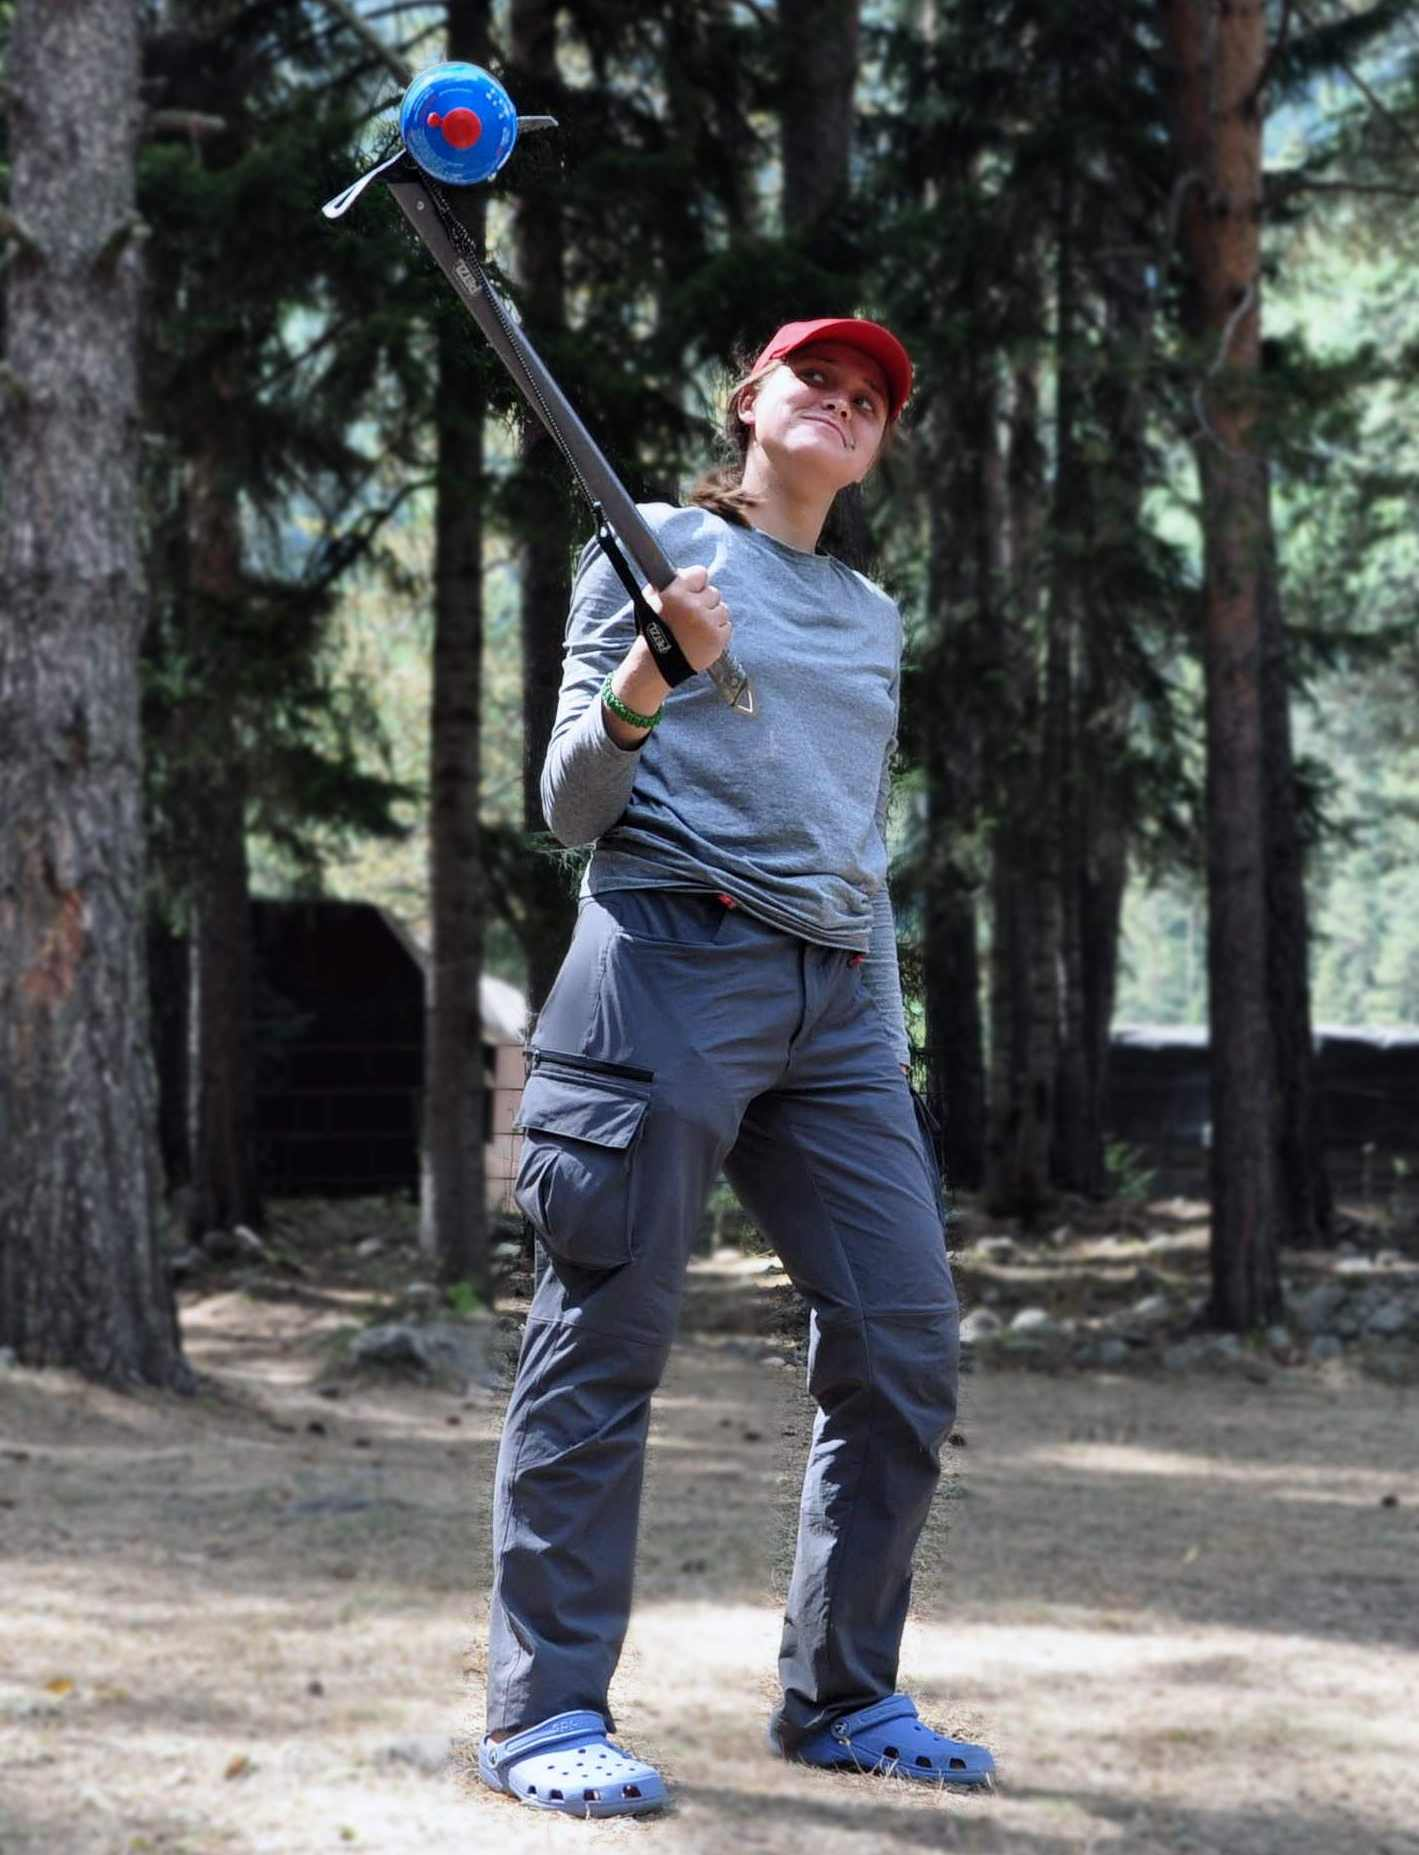
\includegraphics[width=\textwidth]{../pics/DSC_1152}			
		\end{minipage}
		\vfill
	}
\end{frame}

\begin{frame}
	\frametitle{Мост через р. Гондарай}
	\framesubtitle{День 4, 21 августа}
	\centering
	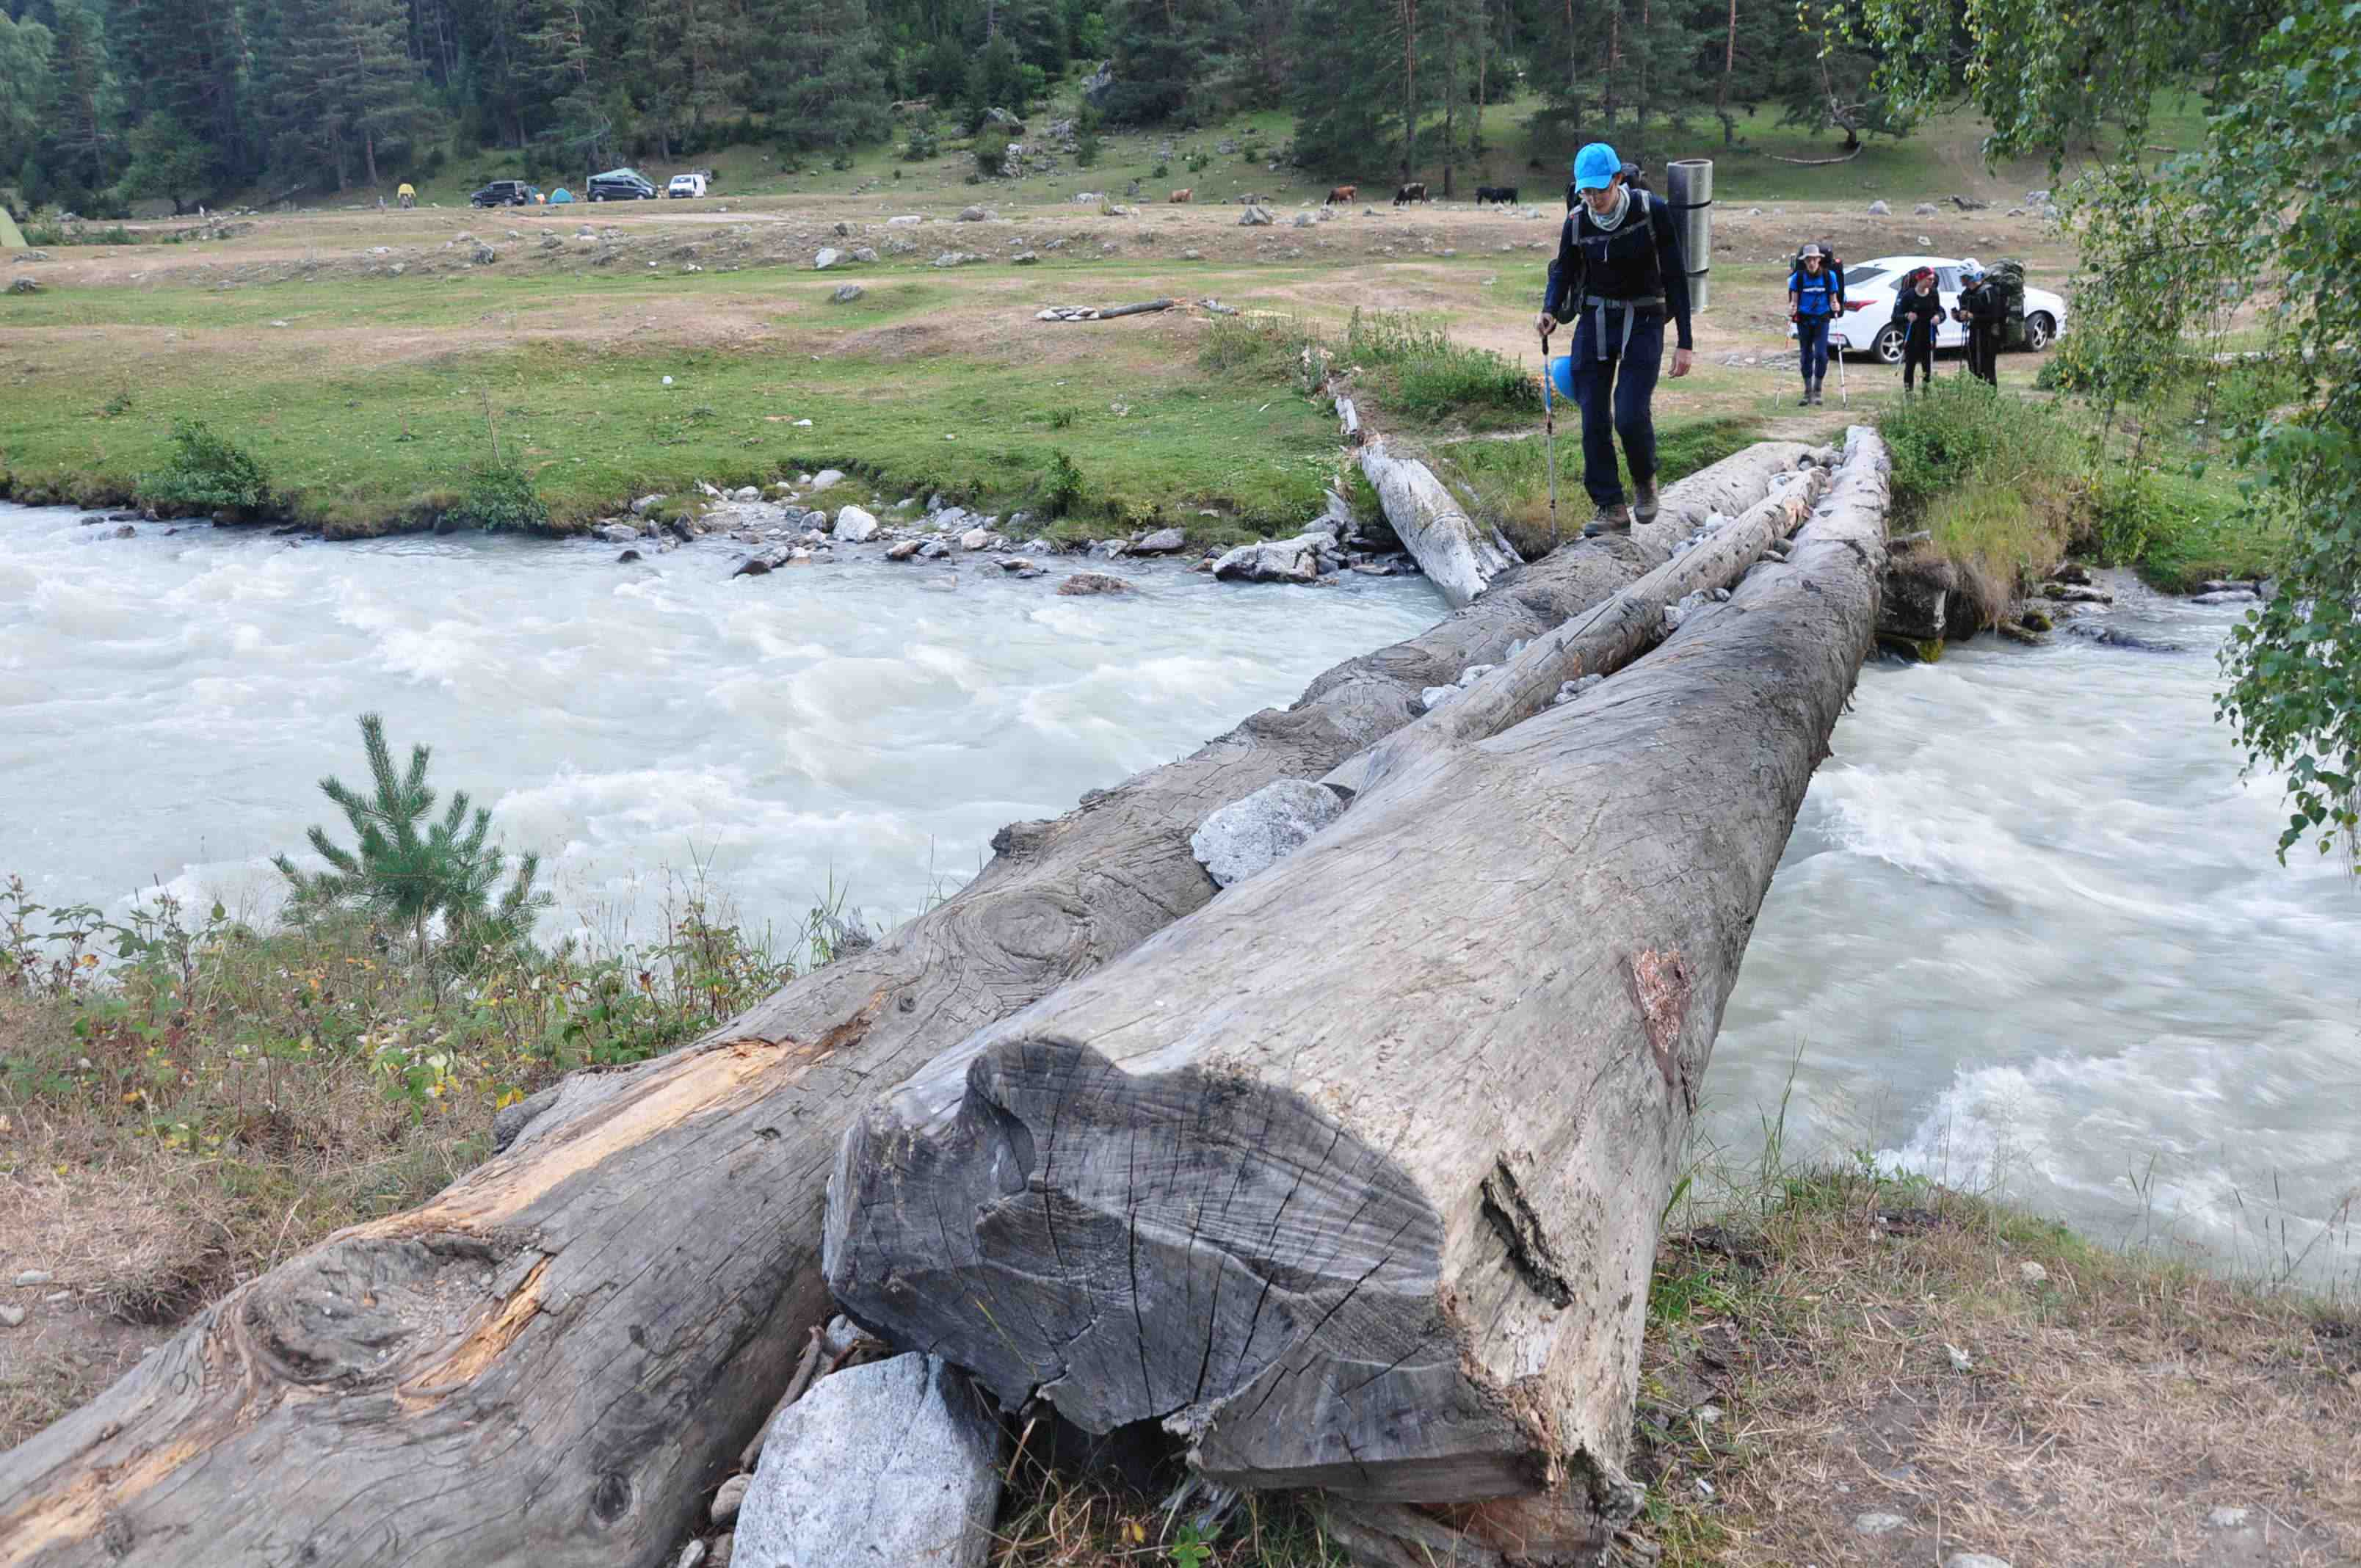
\includegraphics[width=\textwidth]{../pics/DSC_1167}			
\end{frame}

	
		\begin{frame}
	\frametitle{День 5. 22 августа}
	\framesubtitle{д.р. Кичкинекол Джалпаккольский~--- м.н. под моренным валом пер. Джалпаккол Северный} % Optional subtitle
	\begin{columns}[c] % The "c" option specifies centered vertical alignment while the "t" option is used for top vertical alignment
		\begin{column}{0.45\textwidth} % Left column width
			\begin{itemize}
				\item Прохождение каменного лабиринта
				\item Гроза
				\item[]
				\item Прошли \textbf{5.8} км
				\item ЧХВ: 3:56
				\item Набор/сброс: \textcolor{darkred}{\textbf{+620}}/\textcolor{darkblue}{\textbf{-0}}~м
			\end{itemize}
			
		\end{column}
		\begin{column}{0.5\textwidth} % Right column width
			\centering
			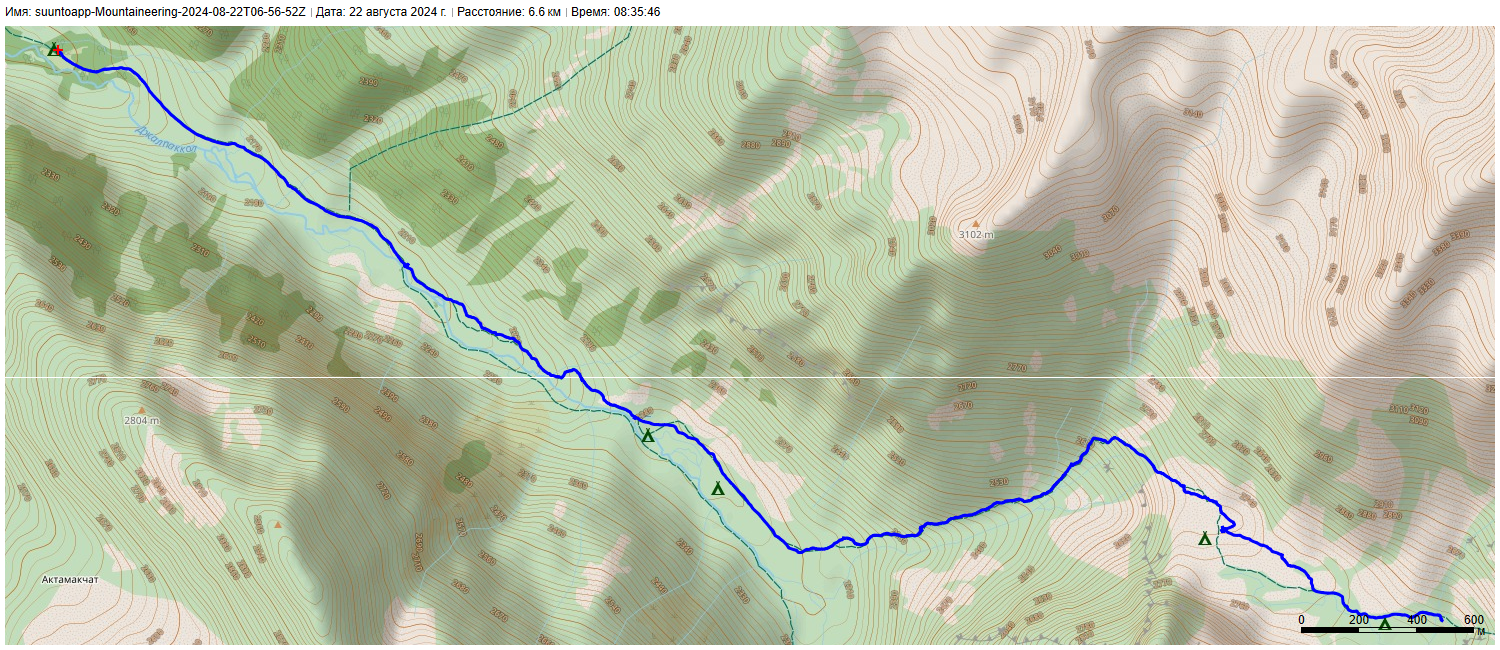
\includegraphics[width=\linewidth]{../pics/mini_maps/22}
		\end{column}
	\end{columns}
\end{frame}




\begin{frame}
	\frametitle{Крокусы в д.р. Джалпаккол}
	\framesubtitle{День 5, 22 августа}
	\footnotesize«Джалпак къол»~--- «Плоское ущелье»
	\centering
	\includegraphics[width=0.85\textwidth]{../pics/IMG_20240822_101607}			
\end{frame}

\begin{frame}
	\frametitle{Поворот в д.р. Кичкинекол Джалпаккольский}
	\framesubtitle{День 5, 22 августа}
	\centering
	\includegraphics[width=\textwidth]{../pics/DJI_0835}			
\end{frame}


\begin{frame}
	\frametitle{\textAlpha\textpi \textomikron\textkappa\textalpha\textlambda\textnu\textpsi\textiota\textvarsigma}
	\framesubtitle{День 5, 22 августа}
	\centering
	\includegraphics[width=\textwidth]{../pics/DSC_0010}			
\end{frame} 

\begin{frame}
	\frametitle{\textAlpha\textpi \textomikron\textkappa\textalpha\textlambda\textnu\textpsi\textiota\textvarsigma}
	\framesubtitle{День 5, 22 августа}
		{\tiny
		\begin{minipage}{\fourpicsize}
			\centering
			\includegraphics[width=\textwidth]{../pics/IMG_20240822_182758}			
		\end{minipage}
		\hfill
		\begin{minipage}{\fourpicsize}
			\centering
			\includegraphics[width=\textwidth]{../pics/IMG_20240822_193315}			
		\end{minipage}
		\vfill
		}			
\end{frame} 



		\begin{frame}
	\frametitle{День 6. 23 августа}
	\framesubtitle{\textbf{пер. Джалпаккол Северный (1А$^\star$, 3411)}~--- зелёные ночёвки на спуске в д.р. Мырды} % Optional subtitle
	\begin{columns}[c] % The "c" option specifies centered vertical alignment while the "t" option is used for top vertical alignment
		\begin{column}{0.55\textwidth} % Left column width
			\begin{itemize}
				\item Собирались 3 часа
				\item Руковод пропитался какао
				\item У Наташи убились колени$\,\to\,$угроза схода второго участника
				\item Взяли перевал
				\item Спускались в тумане по приборам (обещанный вайб Silent Hill)
				\item Катарсис
				\item Прошли \textbf{5.0} км
				\item ЧХВ: 6:16
				\item Набор/сброс: \textcolor{darkred}{\textbf{+660}}/\textcolor{darkblue}{\textbf{-395}}~м
			\end{itemize}
			
		\end{column}
		\begin{column}{0.45\textwidth} % Right column width
			\centering
			\includegraphics[width=\linewidth]{../pics/mini_maps/23}
		\end{column}
	\end{columns}
\end{frame}

\begin{frame}
	\frametitle{Перевальный взлёт}
	\framesubtitle{День 6, 23 августа}
	\centering
	\includegraphics[width=\textwidth]{../pics/dzh_1}			
\end{frame}



\begin{frame}
	\frametitle{Группа в снежном кармане перед скальным участком перевала}
	\framesubtitle{День 6, 23 августа}
	\centering
	\includegraphics[width=\textwidth]{../pics/DSC_0021}			
\end{frame}


\begin{frame}
	\frametitle{Подъём на гребень}
	\framesubtitle{День 6, 23 августа}
	\centering
	\includegraphics[width=\textwidth]{../pics/DSC_0029}			
\end{frame}

\begin{frame}
	\frametitle{Группа на пер. Джалпаккол Северный (1А$^\star$)}
	\framesubtitle{День 3, 20 августа}
	{\tiny
		\begin{minipage}{\fourpicsize}
			\centering
			\includegraphics[width=\textwidth]{../pics/DSC_0063}			
			Вид в д.р. Мырды (хоть этого и не видно)
		\end{minipage}
		\hfill
		\begin{minipage}{\fourpicsize}
			\centering
			\includegraphics[width=\textwidth]{../pics/DSC_0069}			
			Вид в д.р. Кичкинекол Джалпаккольский
		\end{minipage}
		\vfill
	}
\end{frame}

\begin{frame}
	\frametitle{Гребень}
	\framesubtitle{День 6, 23 августа}
	\centering
	\includegraphics[width=\textwidth]{../pics/DSC_0047}			
\end{frame}

\begin{frame}
	\frametitle{Спуск к озеру}
	\framesubtitle{День 6, 23 августа}
	\centering
	\includegraphics[width=\textwidth]{../pics/DSC_0041}			
\end{frame}


\begin{frame}
	\frametitle{Туман на озере}
	\framesubtitle{День 6, 23 августа}
	\centering
	\includegraphics[width=\textwidth]{../pics/DSC_0089}			
\end{frame}

\begin{frame}
	\frametitle{Ранние сумерки}
	\framesubtitle{День 6, 23 августа}
	\centering
	\includegraphics[width=\textwidth]{../pics/DSC_0094}			
\end{frame}

\begin{frame}
	\frametitle{Ещё туман}
	\framesubtitle{День 6, 23 августа}
	\centering
	\includegraphics[width=\textwidth]{../pics/DSC_0095}			
\end{frame}

\begin{frame}
	\frametitle{Вайбовый вайб}
	\framesubtitle{День 6, 23 августа}
	\centering
	\includegraphics[width=\textwidth]{../pics/IMG_20240823_184041}			
\end{frame}

		\begin{frame}
	\frametitle{День 7. 24 августа}
	\framesubtitle{д.р. Мырды~--- а/л <<Узункол>>	} % Optional subtitle
	\begin{columns}[c] % The "c" option specifies centered vertical alignment while the "t" option is used for top vertical alignment
		\begin{column}{0.55\textwidth} % Left column width
			\begin{itemize}
				\item Альплагерь «Узункол» («Длинное ущелье»)
				\item Группа и баня
				\item Прошли \textbf{7.5} км
				\item ЧХВ: 3:53
				\item Набор/сброс: \textcolor{darkred}{\textbf{+0}}/\textcolor{darkblue}{\textbf{-963}}~м
			\end{itemize}
			
		\end{column}
		\begin{column}{0.45\textwidth} % Right column width
			\centering
			\includegraphics[width=\linewidth]{../pics/mini_maps/24}
		\end{column}
	\end{columns}
\end{frame}

\begin{frame}
	\frametitle{На спуске в д.р. Мырды}
	\framesubtitle{День 7, 24 августа}
	\centering
	\includegraphics[width=\textwidth]{../pics/DSC_0104}			
\end{frame}

\begin{frame}
	\frametitle{Верховья р. Мырды}
	\framesubtitle{День 7, 24 августа}
	\centering
	\includegraphics[width=\textwidth]{../pics/DSC_0107}			
\end{frame}

\begin{frame}
	\frametitle{В поисках нарзанов}
	\framesubtitle{День 7, 24 августа}
	\centering
	\includegraphics[width=\textwidth]{../pics/DSC_0111}			
\end{frame}

\begin{frame}
	\frametitle{Вид лагеря}
	\framesubtitle{День 7, 24 августа}
	\centering
	\includegraphics[width=\textwidth]{../pics/DSC_0126}			
\end{frame}
		\begin{frame}
	\frametitle{День 8. 25 августа}
	\framesubtitle{д.р. Кичкинекол~--- д.р. Таллычат~--- Поляна Крокусов	} % Optional subtitle
	\begin{columns}[c] % The "c" option specifies centered vertical alignment while the "t" option is used for top vertical alignment
		\begin{column}{0.55\textwidth} % Left column width
			\begin{itemize}
				\item Потерянная ручка
				\item Поляна Крокусов
				\item Гроза
				\item Прошли \textbf{7.1} км
				\item ЧХВ: 3:23
				\item Набор/сброс: \textcolor{darkred}{\textbf{+780}}/\textcolor{darkblue}{\textbf{-0}}~м
			\end{itemize}
			
		\end{column}
		\begin{column}{0.45\textwidth} % Right column width
			\centering
			\includegraphics[width=\linewidth]{../pics/mini_maps/25}
		\end{column}
	\end{columns}
\end{frame}

\begin{frame}
	\frametitle{Руководитель\dots}
	\framesubtitle{День 8, 25 августа}
	\centering
	\includegraphics[width=\textwidth]{../pics/DSC_0128}			
\end{frame}

\begin{frame}
	\frametitle{\dots~и группа}
	\framesubtitle{День 8, 25 августа}
	\centering
	\includegraphics[width=\textwidth]{../pics/DSC_0127}			
\end{frame}

\begin{frame}
\frametitle{Растительность Кавказа}
	\framesubtitle{День 8, 25 августа}
	\centering
	\includegraphics[width=\textwidth]{../pics/DSC_0143}			
\end{frame}

\begin{frame}
	\frametitle{Осень в горах}
	\framesubtitle{День 8, 25 августа}
	\centering
	\includegraphics[width=\textwidth]{../pics/DSC_0149}			
\end{frame}

\begin{frame}
	\frametitle{Тоска по потерянной ручке}
	\framesubtitle{День 8, 25 августа}
	\centering
	\includegraphics[width=\textwidth]{../pics/DSC_0155}			
\end{frame}

\begin{frame}
	\frametitle{Вершины и перевалы ГКХ в районе пер. Кичкинекол}
	\framesubtitle{День 8, 25 августа}
	\centering
	\includegraphics[width=\textwidth]{../pics/DSC_0158}			
\end{frame}

\begin{frame}
	\frametitle{Поляна Крокусов}
	\framesubtitle{День 8, 25 августа}
	\centering
	\includegraphics[width=\textwidth]{../pics/DSC_0177}			
\end{frame}

\begin{frame}
	\frametitle{Туман \textbf{не} сел}
	\framesubtitle{День 8, 25 августа}
	\centering
	\includegraphics[width=\textwidth]{../pics/DSC_0179}			
\end{frame}

\begin{frame}
	\frametitle{Туман сел}
	\framesubtitle{День 8, 25 августа}
	\centering
	\includegraphics[width=\textwidth]{../pics/DSC_0181}			
\end{frame}

\begin{frame}
	\frametitle{Квартир\dots~палаточник}
	\framesubtitle{День 8, 25 августа}
	\centering
	\includegraphics[width=\textwidth]{../pics/DSC_0187}			
\end{frame}
		\begin{frame}
	\frametitle{День 9. 26 августа}
	\framesubtitle{\textbf{пер. Кичкинекол Малый (1А, 3206)}~--- д.р. Чунгур-Джар} % Optional subtitle
	\begin{columns}[c] % The "c" option specifies centered vertical alignment while the "t" option is used for top vertical alignment
		\begin{column}{0.55\textwidth} % Left column width
			\begin{itemize}
				\item «Самый лайтовый перевал»
				\item Поляна Крокусов
				\item Гроза
				\item Прошли \textbf{4.6} км
				\item ЧХВ: 2:42
				\item Набор/сброс: \textcolor{darkred}{\textbf{+360}}/\textcolor{darkblue}{\textbf{-520}}~м
			\end{itemize}
			
		\end{column}
		\begin{column}{0.45\textwidth} % Right column width
			\centering
			\includegraphics[width=\linewidth]{../pics/mini_maps/26}
		\end{column}
	\end{columns}
\end{frame}

\begin{frame}
	\frametitle{Утро}
	\framesubtitle{День 9, 26 августа}
	\centering
	\includegraphics[width=\textwidth]{../pics/DSC_0190}			
\end{frame}

\begin{frame}
	\frametitle{Круг камней}
	\framesubtitle{День 9, 26 августа}
	\centering
	\includegraphics[width=\textwidth]{../pics/DSC_0192}			
\end{frame}

\begin{frame}
	\frametitle{Козлы}
	\framesubtitle{День 9, 26 августа}
	\centering
	\includegraphics[width=\textwidth]{../pics/DSC_0211}			
\end{frame}

\begin{frame}
	\frametitle{Атмосфера дня}
	\framesubtitle{День 9, 26 августа}
	\centering
	\includegraphics[width=\textwidth]{../pics/DSC_0222}			
\end{frame}

\begin{frame}
	\frametitle{Маршрут движения группы}
	\framesubtitle{День 9, 26 августа}
	\centering
	\includegraphics[width=\textwidth]{../pics/DSC_0226}			
\end{frame}


\begin{frame}
	\frametitle{Группа на пер. Кичкинекол Малый (1А)}
	\framesubtitle{День 9, 26 августа}
	{\tiny
		\begin{minipage}{\fourpicsize}
			\centering
			\includegraphics[width=\textwidth]{../pics/DSC_0239}			
			Вид в д.р. Чунгур-Джар
		\end{minipage}
		\hfill
		\begin{minipage}{\fourpicsize}
			\centering
			\includegraphics[width=\textwidth]{../pics/DSC_0242}			
			Вид в д.р. Таллычат
		\end{minipage}
		\vfill
	}
\end{frame}
		\begin{frame}
	\frametitle{День 10. 27 августа}
	\framesubtitle{\textbf{пер. Перемётный (1А, 3255)}~--- д.р. Танышхан} % Optional subtitle
	\begin{columns}[c] % The "c" option specifies centered vertical alignment while the "t" option is used for top vertical alignment
		\begin{column}{0.55\textwidth} % Left column width
			\begin{itemize}
				\item Куда укажет флюгер
				\item Клад для руковода
				\item Косяк руковода
				\item Первая кровь
				\item Тот самый спуск с Перемётного
				\item Последствия ошибки руковода
				\item Прошли \textbf{7.1} км
				\item ЧХВ: 6:50
				\item Набор/сброс: \textcolor{darkred}{\textbf{+575}}/\textcolor{darkblue}{\textbf{-935}}~м
			\end{itemize}
			
		\end{column}
		\begin{column}{0.45\textwidth} % Right column width
			\centering
			\includegraphics[width=\linewidth]{../pics/mini_maps/27}
		\end{column}
	\end{columns}
\end{frame}

\begin{frame}
	\frametitle{Стойбище}
	\framesubtitle{День 10, 27 августа}
	\centering
	\includegraphics[width=\textwidth]{../pics/DSC_0252}			
\end{frame}

\begin{frame}
	\frametitle{р. Чунгур-Джар. Нам предстоит перебраться через множество ручейков}
	\framesubtitle{День 10, 27 августа}
	\centering
	\includegraphics[width=\textwidth]{../pics/DSC_0254}			
\end{frame}

\begin{frame}
	\frametitle{Начало подъёма к пер. Перемётный из д.р. Чунгур-Джар}
	\framesubtitle{День 10, 27 августа}
	\centering
	\includegraphics[width=\textwidth]{../pics/perem_1}			
\end{frame}

\begin{frame}
	\frametitle{Траверс по моренам и выход на моренный гребень}
	\framesubtitle{День 10, 27 августа}
	\centering
	\includegraphics[width=\textwidth]{../pics/DSC_0280}			
\end{frame}

\begin{frame}
	\frametitle{Перевальный взлёт}
	\framesubtitle{День 10, 27 августа}
	\centering
	\includegraphics[width=\textwidth]{../pics/DSC_0341}			
\end{frame}

\begin{frame}
	\frametitle{Группа на пер. Перемётный (1А)}
	\framesubtitle{День 10, 27 августа}
	{\tiny
		\begin{minipage}{\fourpicsize}
			\centering
			\includegraphics[width=\textwidth]{../pics/DSC_0412 2.jpg}			
			Вид в д.р. Чунгур-Джар
		\end{minipage}
		\hfill
		\begin{minipage}{\fourpicsize}
			\centering
			\includegraphics[width=\textwidth]{../pics/DSC_0419 2.jpg}			
			Вид в д.р. Танышхан
		\end{minipage}
		\vfill
	}
\end{frame}

\begin{frame}
	\frametitle{Фотоньки с перевала}
	\framesubtitle{День 10, 27 августа}
	\centering
	\includegraphics[width=\textwidth]{../pics/DSC_0369 2}			
\end{frame}

\begin{frame}
	\frametitle{Фотоньки с перевала}
	\framesubtitle{День 10, 27 августа}
	\centering
	\includegraphics[width=\textwidth]{../pics/DSC_0385 2}			
\end{frame}


\begin{frame}
	\frametitle{Готовность к спуску}
	\framesubtitle{День 10, 27 августа}
	\centering
	\includegraphics[width=\textwidth]{../pics/DSC_0428 2}			
\end{frame}

\begin{frame}
	\frametitle{Спуск к «анучинским» ночёвкам на 2900 м}
	\framesubtitle{День 10, 27 августа}
	\centering
	\includegraphics[width=\textwidth]{../pics/DSC_0425 2}			
\end{frame}

\begin{frame}
	\frametitle{Спуск к «анучинским» ночёвкам на 2900 м}
	\framesubtitle{День 10, 27 августа}
	\centering
	\includegraphics[width=\textwidth]{../pics/DSC_0430 2}			
\end{frame}

\begin{frame}
	\frametitle{Движение по курумнику. Фото Анучиной Светланы}
	\framesubtitle{День 10, 27 августа}
	\footnotesize Красная линия~--- наш трек
	\centering
	\includegraphics[width=\textwidth]{../pics/peremkurum.png}			
\end{frame}


	\begin{frame}
	\frametitle{День 11. 28 августа}
	\framesubtitle{д.р. Чиринкол~--- д.р. Кубань} % Optional subtitle
	\begin{columns}[c] % The "c" option specifies centered vertical alignment while the "t" option is used for top vertical alignment
		\begin{column}{0.55\textwidth} % Left column width
			\begin{itemize}
				\item Четверо сходят
				\item Солнышко светит
				\item Лёша психанул
				\item Прошли \textbf{12.7} км
				\item ЧХВ: 3:23
				\item Набор/сброс: \textcolor{darkred}{\textbf{+90}}/\textcolor{darkblue}{\textbf{-500}}~м
			\end{itemize}			
		\end{column}
		\begin{column}{0.45\textwidth} % Right column width
			\centering
			\includegraphics[width=\linewidth]{../pics/mini_maps/28}
		\end{column}
	\end{columns}
\end{frame}

\begin{frame}
	\frametitle{Настроение руководителя}
	\framesubtitle{День 11, 28 августа}	
	\centering
	\includegraphics[width=\textwidth]{../pics/DSC_0435 2}			
\end{frame}

\begin{frame}
	\frametitle{Руководы}
	\framesubtitle{День 11, 28 августа}	
	\centering
	\includegraphics[width=\textwidth]{../pics/DSC_0455 2}			
\end{frame}

\begin{frame}
	\frametitle{Д.р. Чунгур-Джар}
	\framesubtitle{День 11, 28 августа}	
	\footnotesize Именно эти ступени мы обходили через пер. Перемётный
	\centering
	\includegraphics[width=0.95\textwidth]{../pics/DSC_0459 2}			
\end{frame}

\begin{frame}
	\frametitle{Вид д.р. Чиринкол}
	\framesubtitle{День 11, 28 августа}	
	\footnotesize«Чирин къол»~--- «Гнилое ущелье»
	\centering
	\includegraphics[width=0.9\textwidth]{../pics/DSC_0461 2}			
\end{frame}

\begin{frame}
	\frametitle{Вид д.р. Чиринкол}
	\framesubtitle{День 11, 28 августа}	
	\centering
	\includegraphics[width=0.45\textwidth]{../pics/DSC_0460 2}			
\end{frame}

\begin{frame}
	\frametitle{Вилка долин}
	\framesubtitle{День 11, 28 августа}	
	\centering
	\includegraphics[width=\textwidth]{../pics/DSC_0462 2}			
\end{frame}

	\begin{frame}
	\frametitle{День 12. 29 августа}
	\framesubtitle{погранзастава <<Хурзук>>~(рад.)~--- д.р. Уллу-Кам} % Optional subtitle
	\begin{columns}[c] % The "c" option specifies centered vertical alignment while the "t" option is used for top vertical alignment
		\begin{column}{0.55\textwidth} % Left column width
			\begin{itemize}
				\item Марш-бросок к погранзаставе
				\item Подъём к Хотютау
				\item Примета: увидеть конных погранцов в камере дрона~--- не к добру
				\item Катарсис
				\item Прошли \textbf{20.9} км
				\item ЧХВ: 7:15
				\item Набор/сброс: \textcolor{darkred}{\textbf{+1210}}/\textcolor{darkblue}{\textbf{-370}}~м
			\end{itemize}			
		\end{column}
		\begin{column}{0.45\textwidth} % Right column width
			\centering
			\includegraphics[width=\linewidth]{../pics/mini_maps/29}
		\end{column}
	\end{columns}
\end{frame}

\begin{frame}
	\frametitle{д.р. Кубань, вид с подъёма в д.р. Уллу-Кам}
	\framesubtitle{День 12, 29 августа}	
	\centering
	\includegraphics[width=\textwidth]{../pics/DSC_0464 2}			
\end{frame}

\begin{frame}
	\frametitle{Можжевеловое}
	\framesubtitle{День 12, 29 августа}	
	\centering
	\includegraphics[width=\textwidth]{../pics/DSC_0471 2}			
\end{frame}

\begin{frame}
	\frametitle{Когда не зря}
	\framesubtitle{День 12, 29 августа}	
	\footnotesize Єльбрус (кродёться)
	\centering
	\includegraphics[width=\textwidth]{../pics/IMG_20240829_170756}			
\end{frame}

\begin{frame}
	\frametitle{Вид на Эльбрус с м.н.}
	\framesubtitle{День 12, 29 августа}	
	\centering
	\includegraphics[width=\textwidth]{../pics/IMG_20240829_181353}			
\end{frame}

\begin{frame}
	\frametitle{Место ночёвки 29-30 августа}
	\framesubtitle{День 12, 29 августа}	
	\centering
	\includegraphics[width=\textwidth]{../pics/IMG_20240829_191225}			
\end{frame}


	\begin{frame}
	\frametitle{День 12. 29 августа}
	\framesubtitle{\textbf{пер. Хотютау (1А$^\star$, 3546)}~--- лед. Большой Азау~--- оз. Эльбрусское~--- ст. <<Старый Кругозор>>~--- поляна Азау} % Optional subtitle
	\begin{columns}[c] % The "c" option specifies centered vertical alignment while the "t" option is used for top vertical alignment
		\begin{column}{0.55\textwidth} % Left column width
			\begin{itemize}
				\item Последнее усилие
				\item Туристы из т/к МАИ
				\item Ошибка штурмана
				\item Alpindustria Elbrus \textit{«Heavy Ryukzak»} Race
				\item Прошли \textbf{10.9} км
				\item ЧХВ: 4:25
				\item Набор/сброс: \textcolor{darkred}{\textbf{+800}}/\textcolor{darkblue}{\textbf{-615}}~м
			\end{itemize}			
		\end{column}
		\begin{column}{0.45\textwidth} % Right column width
			\centering
			\includegraphics[width=\linewidth]{../pics/mini_maps/30}
		\end{column}
	\end{columns}
\end{frame}


\begin{frame}
	\frametitle{Утренний вид на юго-западные склоны Эльбруса}
	\framesubtitle{День 13, 30 августа}	
	\centering
	\includegraphics[width=\textwidth]{../pics/IMG_20240830_063548}			
\end{frame}

\begin{frame}
	\frametitle{Путь подъёма}
	\framesubtitle{День 13, 30 августа}	
	\centering
	\includegraphics[width=0.8\textwidth]{../pics/IMG_20240830_105443}			
\end{frame}

\begin{frame}
	\frametitle{Группа на пер. Хотютау (1А, 3546)}
	\framesubtitle{День 13, 30 августа}	
	\centering
	\includegraphics[width=\textwidth]{../pics/DJI_0899}			
\end{frame}

\begin{frame}
	\frametitle{На леднике}
	\framesubtitle{День 10, 27 августа}
	{\scriptsize
		\begin{minipage}{\fourpicsize}
			\centering
			\includegraphics[width=0.9\textwidth]{../pics/20240830_141852.jpg}			
			Группа на леднике. Фото туристов т/к МАИ
		\end{minipage}
		\hfill
		\begin{minipage}{\fourpicsize}
			\centering
			\includegraphics[width=0.9\textwidth]{../pics/20240830_155136.jpg}			
			Единственный раз, когда собакам действительно пригодились ботинки
		\end{minipage}
		\vfill
	}
\end{frame}

\begin{frame}
	\frametitle{Где-то у Эльбрусского озера}
	\framesubtitle{День 13, 30 августа}	
	\centering
	\includegraphics[width=\textwidth]{../pics/20240830_162252}			
\end{frame}

\begin{frame}
	\frametitle{Валим вниз}
	\framesubtitle{День 13, 30 августа}
	\scriptsize А собачки постигают новый для себя вид транспорта
	\centering
	\includegraphics[width=0.55\textwidth]{../pics/IMG_20240830_170232}			
\end{frame}

\begin{frame}
	\frametitle{Конец путешествия, поляна Азау}
	\framesubtitle{День 13, 30 августа}	
	\centering
	\includegraphics[width=\textwidth]{../pics/group_finish.jpg}			
\end{frame}
	\section{Результаты}
\begin{frame}
	
	\frametitle[	содержимое...]{Результаты в цифрах}
	\begin{itemize}
		\item<+-> Пройдено \textbf{111} км за \textbf{13} ходовых дней
		\item<+-> Получился такой высотный график:
		\item<+-> Граммовка раскладки~--- в среднем \textbf{500} граммов на человека в день
		\item<+-> Продолбано \textbf{6} участников из 12
		\item<+->Средний расход аптечки:
	\end{itemize}
	
	\only<2>{
		\begin{center}
			\includegraphics[width=\textwidth]{../pics/elevation_vs_distance}
		\end{center}
		\vfil
	}
\end{frame}


	
	\section{Выводы}
	
	%------------------------------------------------
	
	\begin{frame}[plain] % The optional argument 'plain' hides the headline and footline
		\begin{center}
			{\Huge The End}
			
			\bigskip\bigskip % Vertical whitespace
			
			{\LARGE Questions? Comments?}
		\end{center}
	\end{frame}
	
	%----------------------------------------------------------------------------------------
	
\end{document} 